\documentclass[11pt]{article}
\usepackage[margin=1.1in]{geometry}
\usepackage{amsmath,amssymb,amsthm}
\usepackage{booktabs}
\usepackage{array}
\usepackage[hidelinks]{hyperref}
\usepackage{orcidlink}
\usepackage{xcolor}
% The algorithm float comes from newfloat, as in the other manuscripts of the programme: the algorithm package redefines the
% caption machinery of every float and doubles the hyperref anchors.
\usepackage{newfloat}
\usepackage{placeins}
\DeclareFloatingEnvironment[name=Algorithm,fileext=loa]{algorithm}
\usepackage[noend]{algpseudocode}
\usepackage{tikz}
\usetikzlibrary{arrows.meta}
\usepackage{pgfplots}
\usepgfplotslibrary{groupplots}
\pgfplotsset{compat=1.16}
\emergencystretch=3em
\setlength{\tabcolsep}{4pt}
\makeatletter\g@addto@macro{\UrlBreaks}{\do\-\do\_}\makeatother

\newtheorem{theorem}{Theorem}
\newtheorem{thmletter}{Theorem}
\renewcommand{\thethmletter}{\Alph{thmletter}}
\newtheorem{proposition}{Proposition}
\newtheorem{lemma}{Lemma}
\newtheorem{corollary}{Corollary}
\theoremstyle{definition}
\newtheorem{definition}{Definition}
\theoremstyle{remark}
\newtheorem{remark}{Remark}
\newcommand{\doi}[1]{\href{https://doi.org/#1}{doi:#1}}
\newcommand{\EXP}[1]{\mbox{EXP-#1}}
\newcommand{\Q}{\mathbb{Q}}
\newcommand{\F}{\mathbb{F}}
\newcommand{\Z}{\mathbb{Z}}
\newcommand{\Ext}{\operatorname{Ext}}
\newcommand{\Tor}{\operatorname{Tor}}
\newcommand{\Proj}{\operatorname{Proj}}
\newcommand{\Hilb}{\operatorname{HS}}
\newcommand{\ch}{\operatorname{char}}
% Generated by make_tables.py from the archived computations. Do not edit.
\newcommand{\nafterOneAOpen}{120}
\newcommand{\nagreeThree}{127}
\newcommand{\nagreeTwo}{96}
\newcommand{\nbOneEightFour}{26}
\newcommand{\nbOneEightSixteen}{40}
\newcommand{\nbOneEightTwo}{9}
\newcommand{\nbOneFiveEightFour}{19}
\newcommand{\nbOneFiveEightSixteen}{33}
\newcommand{\nbOneFiveEightTwo}{3}
\newcommand{\nbOneSeedsCharTwo}{40}
\newcommand{\nbOneSeedsControl}{20}
\newcommand{\nbOneSixFour}{20}
\newcommand{\nbOneSixSixteen}{38}
\newcommand{\nbOneSixTwo}{12}
\newcommand{\nbetaOneRays}{8}
\newcommand{\nbetaOneRaysDone}{5}
\newcommand{\nblocksChecked}{1{,}715}
\newcommand{\nblocksPrimes}{11}
\newcommand{\ncDetermined}{205}
\newcommand{\ncalibAgree}{17}
\newcommand{\ncalibMaxOne}{0.12}
\newcommand{\ncalibMaxTwo}{1.29}
\newcommand{\ncalibModules}{17}
\newcommand{\ncellSecondsMax}{364}
\newcommand{\ncellSecondsMedian}{0.23}
\newcommand{\ncellSecondsTotal}{20{,}089}
\newcommand{\ncellsErr}{2}
\newcommand{\ncellsHit}{1{,}253}
\newcommand{\ncellsMain}{1046}
\newcommand{\ncellsMiss}{1{,}741}
\newcommand{\ncellsOneE}{1950}
\newcommand{\ncellsTotal}{2{,}996}
\newcommand{\ncentralOneFour}{336}
\newcommand{\ncentralOneTwo}{28}
\newcommand{\ncentralTwoFour}{21}
\newcommand{\ncentralTwoTwo}{7}
\newcommand{\nconflicts}{0}
\newcommand{\ncyclic}{44}
\newcommand{\ndTwoSeeds}{10}
\newcommand{\ndTwoSubs}{2}
\newcommand{\ndetNonzeroFour}{326}
\newcommand{\ndetNonzeroTwo}{22}
\newcommand{\ndetZeroFour}{10}
\newcommand{\ndetZeroTwo}{6}
\newcommand{\ndiscarded}{59}
\newcommand{\ndualCases}{20}
\newcommand{\ndualHolds}{20}
\newcommand{\nevCubicFour}{39}
\newcommand{\nevCubicSixteen}{40}
\newcommand{\nevCubicTwo}{34}
\newcommand{\nevQuadFour}{39}
\newcommand{\nevQuadSixteen}{40}
\newcommand{\nevQuadTwo}{28}
\newcommand{\nevTwoGFtwo}{29}
\newcommand{\nexcluded}{12}
\newcommand{\nexcludedParityFail}{2}
\newcommand{\nexcludedParityPass}{10}
\newcommand{\nfamilyMaxE}{8}
\newcommand{\nfamilyPiecesEFour}{37}
\newcommand{\nfamilySecondsMax}{12.6}
\newcommand{\nfigPrimeOnly}{46}
\newcommand{\nflagFive}{130}
\newcommand{\nflagGen}{130}
\newcommand{\nflagRaysThree}{3}
\newcommand{\nflagRaysTwo}{21}
\newcommand{\nflagSeeds}{650}
\newcommand{\nflagSeedsFive}{479}
\newcommand{\nflagSeedsThree}{359}
\newcommand{\nflagSeedsTwo}{175}
\newcommand{\nflagThree}{126}
\newcommand{\nflagTwo}{98}
\newcommand{\nformulaAny}{24}
\newcommand{\nformulaInf}{3}
\newcommand{\nformulaZero}{8}
\newcommand{\nfourAgree}{842}
\newcommand{\nfourCharZeroAfter}{191}
\newcommand{\nfourCompared}{842}
\newcommand{\nfourHits}{130}
\newcommand{\nfourKnown}{64}
\newcommand{\nfourLargestCols}{2200}
\newcommand{\nfourLargestRows}{2178}
\newcommand{\nfourLenA}{280}
\newcommand{\nfourLenB}{396}
\newcommand{\nfourLongestSec}{647}
\newcommand{\nfourMatrices}{1{,}087}
\newcommand{\nfourMaxSecHit}{654}
\newcommand{\nfourOneCols}{1440}
\newcommand{\nfourOneRows}{1386}
\newcommand{\nfourPassAll}{130}
\newcommand{\nfourPassOne}{129}
\newcommand{\nfourRaysClosure}{44}
\newcommand{\nfourRaysDirect}{23}
\newcommand{\nfourRaysOnly}{46}
\newcommand{\nfourRest}{66}
\newcommand{\nfourRestPass}{65}
\newcommand{\nfourSeeds}{10}
\newcommand{\nfourTotalSec}{1{,}085}
\newcommand{\nfourUnitTests}{42}
\newcommand{\ngateSevenES}{15400}
\newcommand{\ngateThreeEach}{18}
\newcommand{\ngatesPassed}{7}
\newcommand{\ngeneralPairs}{5}
\newcommand{\ngeneralPureFourFiveTen}{0}
\newcommand{\ngeneralPureTwoThree}{5}
\newcommand{\ngfEightyOneHits}{17}
\newcommand{\ngfNineFinite}{20}
\newcommand{\ngfNineHits}{18}
\newcommand{\ngfThreeHits}{3}
\newcommand{\ngfTwentySevenHits}{16}
\newcommand{\ngrowGFtwo}{6}
\newcommand{\nhitFiles}{1{,}253}
\newcommand{\nhitsFlag}{1013}
\newcommand{\nhitsMain}{240}
\newcommand{\nhitsOneA}{14}
\newcommand{\nhitsOneB}{162}
\newcommand{\nhitsOneC}{64}
\newcommand{\nkostantCount}{15}
\newcommand{\nlowNineAny}{26}
\newcommand{\nlowNineDual}{13}
\newcommand{\nlowNineEvery}{29}
\newcommand{\nlowNineExcluded}{5}
\newcommand{\nlowNineFormula}{35}
\newcommand{\nlowNineInfinite}{3}
\newcommand{\nlowNineModule}{15}
\newcommand{\nlowNineScaling}{2}
\newcommand{\nlowNineSocle}{14}
\newcommand{\nlowNineZero}{50}
\newcommand{\nnormalOrderingCount}{100}
\newcommand{\nnumeratorE}{12}
\newcommand{\noneIdealDims}{2, 4, 8, 12}
\newcommand{\nopen}{15}
\newcommand{\nopenMaxUp}{21}
\newcommand{\nopenParityZero}{1}
\newcommand{\npairsCharThree}{80}
\newcommand{\npairsCharThreeHits}{54}
\newcommand{\npairsCharTwo}{80}
\newcommand{\npairsCharTwoFinite}{0}
\newcommand{\npairsRightHF}{60}
\newcommand{\npairsRightHFWrongTable}{6}
\newcommand{\nparityPassing}{29}
\newcommand{\npbwIdentities}{6}
\newcommand{\nprimePointsNonpure}{13}
\newcommand{\nprimePointsPure}{23}
\newcommand{\nqqCompleted}{64}
\newcommand{\nqqDualsClosure}{2}
\newcommand{\nqqDualsDirect}{11}
\newcommand{\nqqDualsPure}{12}
\newcommand{\nqqFailed}{2}
\newcommand{\nqqFileCount}{32}
\newcommand{\nqqModules}{30}
\newcommand{\nqqNotRun}{57}
\newcommand{\nqqOk}{64}
\newcommand{\nqqPure}{30}
\newcommand{\nqqRays}{29}
\newcommand{\nqqTimeout}{7}
\newcommand{\nqqWithDual}{14}
\newcommand{\nrays}{220}
\newcommand{\nraysLeNine}{84}
\newcommand{\nrealized}{193}
\newcommand{\nrealizedEvery}{52}
\newcommand{\nrealizedPrimeOnly}{46}
\newcommand{\nrealizedZero}{147}
\newcommand{\nrealizedZeroOnly}{95}
\newcommand{\nsearchWallMin}{16}
\newcommand{\nsoderbergPure}{55}
\newcommand{\nsoderbergRays}{55}
\newcommand{\nsourcesArchived}{15}
\newcommand{\nstageZeroEvery}{52}
\newcommand{\nstageZeroOpen}{130}
\newcommand{\nstageZeroRealized}{78}
\newcommand{\nstageZeroWeyman}{26}
\newcommand{\nsubGFfour}{357}
\newcommand{\nsubGFsixteen}{200}
\newcommand{\nsubGFtwo}{35}
\newcommand{\nsubGFtwofiftysix}{200}
\newcommand{\ntenRays}{10}
\newcommand{\nthmRays}{3}
\newcommand{\nthreeCalib}{11}
\newcommand{\nthreeSecA}{488}
\newcommand{\nthreeSecB}{552}
\newcommand{\nthreeSecC}{62}
\newcommand{\nthreeSecD}{184}
\newcommand{\nthreeWall}{151.5}
\newcommand{\ntwoLengths}{27}
\newcommand{\ntwoPairs}{96}
\newcommand{\ntwoWall}{227}
\newcommand{\nuCharTwoDone}{6}
\newcommand{\nuCharTwoExcl}{3}
\newcommand{\nuCharTwoOpen}{1}
\newcommand{\nuEveryCount}{12}
\newcommand{\nuOtherCount}{6}
\newcommand{\nuSquare}{1}
\newcommand{\nverified}{130}


% Page-1 header block (conventions/manuscript-header-standard.md). The four document macros are set by the publishing tool
% when the version DOI is reserved; the version DOI and the concept DOI below are placeholders until the reservation.
\newcommand{\doctype}{Preprint}
\newcommand{\docversion}{v0.03}
\newcommand{\docdate}{20 November 2026}
\newcommand{\versiondoi}{10.5281/zenodo.24385386}
\newcommand{\conceptdoi}{10.5281/zenodo.24385386}
\newcommand{\docrepo}{github.com/fsantibanezleal/CAOS\_RESEARCH}

\newcommand{\headerblock}{%
\begin{center}
\fbox{\parbox{0.94\textwidth}{\small\raggedright
\textbf{\doctype} \quad$\cdot$\quad \docversion, \docdate \quad$\cdot$\quad Licence CC BY 4.0\\[2pt]
CAOS Research open-problems programme \quad$\cdot$\quad problem \texttt{boij-soderberg-realizability}\\[2pt]
Version DOI \href{https://doi.org/\versiondoi}{\texttt{\versiondoi}}\\[2pt]
Concept DOI (always latest) \href{https://doi.org/\conceptdoi}{\texttt{\conceptdoi}}\\[2pt]
Not peer reviewed. Source code, data and computational records: \href{https://\docrepo}{\texttt{\docrepo}}
}}
\end{center}
\vspace{4pt}}

\title{Primitive Betti points over \texorpdfstring{$k[x,y,z]$}{k[x,y,z]} and the Heisenberg enveloping algebra: the point \texorpdfstring{$(1,2,2,1)$}{(1,2,2,1)} on \texorpdfstring{$(0,e,3e,4e)$}{(0,e,3e,4e)} fails only in characteristic \texorpdfstring{$2$}{2} for \texorpdfstring{$2\le e\le10$}{2<=e<=10}, is realized whenever an odd prime \texorpdfstring{$p$}{p} divides \texorpdfstring{$e(e-1)$}{e(e-1)}, and a census for \texorpdfstring{$d_3\le12$}{d3<=12}}
\author{Felipe Santib\'a\~nez-Leal\orcidlink{0000-0002-0150-3246}%
\thanks{\raggedright CAOS open-research programme, Santiago, Chile. Code, computational records and artifacts:
\url{https://github.com/fsantibanezleal/CAOS_RESEARCH}, branch \texttt{develop}, folder
\texttt{problems/commutative-algebra/boij-soderberg-realizability/}.}}
\date{\docdate}

\begin{document}
\maketitle
\headerblock

\begin{abstract}
Erman and Sam asked whether every integral point on a pure ray of the Boij--S\"oderberg cone is the Betti table of a finite length module over $k[x,y,z]$ or over the enveloping algebra $U$ of the Heisenberg Lie algebra; Jiang, Li, Sun, Wang, Xiao and Yu answered negatively. We study the point $(1,2,2,1)$ on $(0,e,3e,4e)$, excluded over $k[x,y,z]$ and passing their test over $U$. It is realized by $U/U(x^e,y^e)$ if and only if $\ch k=0$ or $\ch k\ge2e$, and in characteristic $2$ no module with at most one more relation than generators has finite length over $U$. In odd characteristic $p$ we prove a criterion for pairs of forms with a central commutator, with explicit pure pairs for $e\equiv0,1\pmod p$; such pairs are the images of $(x,y)$ under graded endomorphisms of $U$, which exist only for $p$ dividing $e(e-1)$, and pulling back along them multiplies Betti degrees by $d\equiv0$ or $1\pmod p$. Searches in weight-class strata, a decomposition over $k[xy,z]$, a linear family, a computed filter, lists of forms by one congruence and the stratum with the largest exponent that a weight-zero projection allows give pure pairs over $\F_p$ for the other odd primes below $2e$ when $e\le10$ and $e=12$. For $2\le e\le10$ it is realized over $U$ if and only if $\ch k\ne2$; the pairs \ngridOpenListFourteen{} and those with $e\ge15$ stay open. A census of the \nrays{} rays with $d_3\le12$ over $k[x,y,z]$ realizes the primitive point on \nrealized{} and excludes it on \nexcluded{}; in characteristic $0$ the least counterexample has $d_3=10$.
\end{abstract}

\FloatBarrier
\section{Introduction}
\label{sec:intro}

\subsection{Pure resolutions and the Boij--\texorpdfstring{S\"oderberg}{Soderberg} cone}

Let $S=k[x,y,z]$ with the standard grading and let $M$ be a finitely generated graded $S$-module with minimal graded free resolution $F$. The graded Betti numbers $\beta_{i,j}(M)=\dim_k\Tor_i(M,k)_j$ form the Betti table of $M$. A resolution is pure of type $d=(d_0<d_1<d_2<d_3)$ when the $i$-th free module is generated in the single degree $d_i$. Herzog and K\"uhl showed that the Betti numbers of a finite length module with a pure resolution of type $d$ are proportional to $\prod_{j\ne i}|d_j-d_i|^{-1}$, so that the tables of type $d$ form a ray~\cite{HK84}; the least integral point on the ray is the primitive point $\beta_d$. Boij and S\"oderberg conjectured, and Eisenbud and Schreyer proved, that the Betti tables of finite length modules span a simplicial fan whose extremal rays are exactly these pure rays~\cite{BS08,ES09}; Eisenbud and Schreyer constructed a finite length module with a pure resolution of every type over every field~\cite[Theorem~5.1]{ES09}, and Eisenbud, Fl{\o}ystad and Weyman gave an equivariant construction in characteristic $0$~\cite{EFW11}. Which integral points of a ray occur as Betti tables of modules is a different question. Erman showed that the semigroup of Betti tables of modules is strictly smaller than the semigroup of integral points of the cone: on the ray of $(0,1,3,4)$ the primitive point is not a Betti table although every other integral point is~\cite[Theorem~1.6(1) and its proof]{Erman09}.

\subsection{The question of Erman and Sam and its published answer}

Erman and Sam observed that the primitive point $(1,2,2,1)$ of the ray $(0,1,3,4)$ is realized by the residue field of a noncommutative ring. Let $H$ be the Heisenberg Lie algebra with basis $x,y,z$, bracket $[x,y]=z$, and grading $\deg x=\deg y=1$, $\deg z=2$; its enveloping algebra $U=U(H)$ has the minimal resolution $0\leftarrow U\leftarrow U(-1)^2\leftarrow U(-3)^2\leftarrow U(-4)\leftarrow 0$ of the trivial module, whose Betti table is $(1,2,2,1)$ on $(0,1,3,4)$. They asked~\cite[Question~6.1]{ES16}: \emph{for every degree sequence $(d_0,d_1,d_2,d_3)$ and every integral point on the corresponding ray, is there a finite length module either over $k[x,y,z]$ or over $U(H)$ whose Betti table is that integral point?} They noted that a representation-theoretic construction (Kostant's theorem for the symplectic Lie algebra $\mathfrak{sp}_4$, in which $H$ is the nilradical of a parabolic subalgebra) realizes more such points, with details to appear in forthcoming work of Sam~\cite[Section~6]{ES16}; Kostant's theorem in this setting is stated by Sam~\cite[Theorem~2.1]{Sam15}.

In May 2026 Jiang, Li, Sun, Wang, Xiao and Yu answered the question negatively over every field~\cite[Theorem~3.7]{JLSWXY}. Their example is the degree sequence $(0,6,20,21)$ with the primitive point $(1,2,9,8)$. Over $S$ it is excluded by Krull's height theorem (a cyclic module with two relations has Krull dimension at least $1$). Over $U$ it is excluded by a Hilbert series parity test: the Hilbert series of $U$ is $1/((1-t)^2(1-t^2))$, a finite length module has a polynomial Hilbert series, so the numerator $p(t)=\sum_i(-1)^i\beta_it^{d_i}$ of a pure table must vanish at $t=-1$, and for $(1,2,9,8)$ it takes the value $16$. The polynomial ring half of this argument is an instance of the codimension obstruction of Erman~\cite[Proposition~3.1]{Erman09}, and Boocher, Huang and Wolf classify the rays in three variables with $\beta_1=2$ as a Pell family (their Theorem~15), whose second member is the ray $(0,6,20,21)$ of the example (our reading; the ray is not written there)~\cite{BHW}. The negative answer rests on the numerical parity test, which kills whole rays at once.

\subsection{Results of this paper}
\label{sec:results-list}

The parity test is not the only obstruction to be understood over $U$. We study the primitive points that pass the parity test, that is, the rays on which the numerical test over $U$ is silent, and those among them that are excluded over $S$. The results carry an evidence mark: [MV] machine-verified in the repository by exact arithmetic, [D] derived on paper (here: proved in the paper), [V] read on the primary text, [U] not confirmed, [C] conjectural.
\begin{enumerate}
\item \textbf{A family of pure modules over $U$} (Theorem~\ref{thm:A}). For a field $k$ and $e\ge1$, $M_e=U/U(x^e,y^e)$ has the pure resolution of type $(0,e,3e,4e)$ with Betti numbers $(1,2,2,1)$ if and only if $\ch k=0$ or $\ch k\ge 2e$; then it has length $e^3$ and a one-dimensional socle in degree $4e-4$. [D]; [MV] for $e\le\nfamilyMaxE$ over $\Q$ and for the primes up to $23$ at $e\le5$.
\item \textbf{The characteristic matters} (Theorems~\ref{thm:B} and~\ref{thm:C}). In characteristic $2$ no module over $U$ with $a$ generators in degree $0$ and at most $a+1$ relations, all of one degree $e\ge2$, has finite length. Hence $(1,2,2,1)$ on $(0,e,3e,4e)$ is realized over neither ring in characteristic $2$ for every $e\ge2$, while it is realized over $U$ in characteristic $0$ by $M_e$. [D]; [MV] by exhaustive enumeration over $\F_2$ and $\F_4$ for $e=2$, by searches for $e=2,3$ and the ray $(0,2,10,12)$, and by archived checks on \nfiveExhaustive{} subspaces over $\F_2$ and \nfiveRandom{} random presentations over $\F_2$, $\F_4$ and $\F_{16}$, none of finite length (Section~\ref{sec:resfive}).
\item \textbf{Pairs with a central commutator} (Theorem~\ref{thm:crit}, Corollary~\ref{cor:cases}, Theorem~\ref{thm:central}). In characteristic $p\ge3$, for $f=A+\beta_1x+\beta_2y$ and $g=B+\delta_1x+\delta_2y$ with $A,B,\beta_i,\delta_i$ in the centre $\mathcal Z=k[x^p,y^p,z]$, $gf-fg=-Dz$ is central, and $M=U/(Uf+Ug)$ has finite length if and only if the pair is pure, with an explicit resolution, if and only if $zD$, $n(f)$ and $n(g)$ have no common zero other than the origin. Explicit pure pairs exist for every $e\ge3$ with $e\equiv0$ or $1\pmod p$ (cases A to D), so $(1,2,2,1)$ on $(0,e,3e,4e)$ is realized in characteristic $p$ whenever an odd prime $p$ divides $e(e-1)$; for an odd multiple of $p$ an elementary second proof gives pure pairs with arbitrary central forms. [D]; [MV] on \ncenCases{} central pairs up to $e=15$, \ncritXCases{} explicit pairs of cases B, C, D up to $e=13$ and \ncritRandomPairs{} random pairs of the class, where the criterion and the pure Hilbert function agree on every pair (Sections~\ref{sec:rescen} and~\ref{sec:rescrit}).
\item \textbf{The mechanism and the scaling of Betti tables} (Theorems~\ref{thm:mech} and~\ref{thm:scale}). The explicit sequence of a pair is a complex exactly when the commutator commutes with the pair; those pairs are the images of $(x,y)$ under graded endomorphisms of $U$, a nonzero such commutator is central, and pure pairs of this kind exist only in odd characteristic $p$ dividing $e(e-1)$, never in characteristic $0$ for $e\ge2$. Pulling back along such an endomorphism of degree $d$ multiplies every degree of every Betti table by $d$, so the set of $e$ with $(1,2,2,1)$ realized in characteristic $p$ is closed under multiplication by $d\ge3$ with $d\equiv0$ or $1\pmod p$; this gives the pairs $(8,3)$, $(12,5)$, $(14,3)$, $(16,7)$. [D]; [MV] on \npbCases{} pull-backs, among them the pure pairs of degrees $8$, $12$, $16$ and $24$ (Section~\ref{sec:respull}).
\item \textbf{The weight classes} (Propositions~\ref{prop:strata} and~\ref{prop:pdivm}, Tables~\ref{tab:stratatot} and~\ref{tab:strata}). A pure pair whose forms are homogeneous for the class weight modulo $m$ has a resolution homogeneous for the class, which gives a necessary condition free of the field; the admissible strata and their refinement by containment are computed for $e=4,\dots,8$; and in characteristic $p\le e$ no stratum whose modulus is divisible by $p$ holds a pure pair. [D]; [MV] for the tables.
\item \textbf{Pairs over the invariants} (Proposition~\ref{prop:decomp}, Theorems~\ref{thm:inv}, \ref{thm:cong}, \ref{thm:betti} and~\ref{thm:exist}). For $f=x^e+b\,y^e$ and $g=\Gamma(xy,z)$, $e$ even, the module decomposes over $k[xy,z]$ into $2e$ cyclic modules and its Hilbert function does not depend on $b$; under the hypothesis (C) the pure Hilbert function holds if and only if one congruence modulo $\Gamma$ holds, and then the Betti table is pure; so under (C) the pair is pure exactly when the congruence holds. For every even $e\ge4$ and every prime $p=2e-1$ or $p>2e$ a form with (C) and the congruence exists over a finite field of characteristic $p$ (not necessarily the prime field), and in characteristic $0$ over $k((\nu))$ for any $e/2$ roots among $1,\dots,e$; over an algebraically closed field such forms lie on a curve. At $e=4$ the forms form a quintic curve, with pure pairs over the rationals. [D]; [MV] on the computed cases; [U as archived evidence for the rational pairs].
\item \textbf{Searches in the strata} (Sections~\ref{sec:resstrata} and~\ref{sec:resmid}). The five pairs $(6,5)$, $(6,7)$, $(7,3)$, $(7,5)$, $(7,7)$ have pure pairs over $\F_p$ in admissible strata; at $e=8$ pure pairs over $\F_3$, $\F_5$, $\F_7$, $\F_{11}$, $\F_{13}$; the middle stratum $S(e;0,e/2)$ holds pure pairs at $e=10$ over $\F_3$, $\F_7$, $\F_{11}$, $\F_{13}$ and at $e=12$ over $\F_5$; at $e=9$ pure pairs over $\F_5$, $\F_7$, $\F_{11}$, $\F_{13}$ and $\F_{17}$ (Sections~\ref{sec:resmid} and~\ref{sec:reslinrule}); the stratum of the linear family holds pure pairs at $(10,17)$, $(10,19)$, $(11,19)$, $(12,23)$, $(13,23)$ and none for $2e-p\ge5$, which is proved by the projection on the weight-zero summand (Corollary~\ref{cor:linstratum}); a filter read off computed cases in the stratum $S((e+1)/2;0,(e-1)/2)$ gives pure pairs at $(9,11)$, $(9,13)$, $(11,7)$ and $(13,5)$ (Section~\ref{sec:resfilter}); the lists of forms $\Gamma$ with (C) and the congruence give pure pairs at eleven pairs not settled when the lists were fixed, eight of them settled by no other result, $(12,7)$, $(12,13)$, $(12,17)$, $(12,19)$, $(14,17)$, $(14,19)$, $(16,11)$ and $(16,13)$, and are empty at $(14,5)$ and $(14,11)$ (Section~\ref{sec:reslists}); the stratum with the largest exponent that the weight-zero projection allows, $2t\le p-1$, holds pure pairs at the five pairs $(11,13)$, $(11,17)$, $(13,17)$, $(13,19)$, $(14,23)$, and the stratum with the next exponent holds none with the pure Hilbert function (Section~\ref{sec:reslargest}). Among the \nwcNonAdmMembers{} members examined in the \nwcNonAdm{} strata that are not admissible, none has the pure Hilbert function. [MV]
\item \textbf{The linear family below $2e$} (Section~\ref{sec:reslf}). The four-parameter family $L_e$ holds pure members over $\F_p$ at $(e,p)=(4,5),(4,7),(5,7),(6,11),(7,11),(7,13)$, none for $p\le e$ in the eight pairs computed, and none at $(6,7)$; no member of any of the fifteen pairs below $2e$ has rank of $\mu_{3e}$ above $r$. [MV]
\item \textbf{Odd characteristic below $2e$} (Proposition~\ref{prop:odd}, Corollaries~\ref{cor:ray} and~\ref{cor:eight}, Table~\ref{tab:sixpairs}). Pairs of forms of degree $e$ with the pure table exist over $\F_3$ and $\F_5$ for $e=3$, over $\F_3$, $\F_5$ and $\F_7$ for $e=4$ and for $e=5$, and over $\F_3$ for $e=6$; with the results above, for $2\le e\le10$ the point $(1,2,2,1)$ of $(0,e,3e,4e)$ is realized over $U$ if and only if $\ch k\ne2$. [MV] for the pairs, [D] for the combination with the theorems.
\item \textbf{The state of the point for every $e$ and every odd $p<2e$} (Tables~\ref{tab:state}, \ref{tab:statesrc} and~\ref{tab:statesrcb}, Figure~\ref{fig:grid}). Every pair $(e,p)$ with $p$ dividing $e(e-1)$, with $e=de'$, $d\ge3$, $d\equiv0$ or $1\pmod p$ and $e'$ settled, or with a pure pair found by one of the searches, is settled; \ngridOpen{} of the \ngridCells{} pairs with $e\le16$ stay open, the first being $(11,3)$ at $e=11$; $e=12$ is complete. [D]; [MV] for the pairs taken from computations.
\item \textbf{The locus of pure pairs} (Theorem~\ref{thm:family}, Propositions~\ref{prop:exact} and~\ref{prop:linear}, Tables~\ref{tab:seventangent} and~\ref{tab:sevenpairs}). The two-dimensional spaces $W\subset U_e$ with $U/UW$ pure of type $(0,e,3e,4e)$ are open in a determinantal locus of the multiplication map into degree $3e$, and every component of the pure locus has dimension at least $4e-4$; for $\ch k=0$ or $\ch k\ge2e$ the published modules $U/U(l_1^e,l_2^e)$ form a subfamily of dimension $2$. [D]. Over the rationals the tangent space of the locus at $\langle x^e,y^e\rangle$ has dimension exactly $4e-4$ for $e=4,\dots,7$, so the dimension there is exactly $4e-4$ [MV for the tangent space, D for the consequence], a four-parameter linear family of pairs through $\langle x^e,y^e\rangle$ lies in the locus for every $e\ge4$ in characteristic $0$ or at least $2e$, and its general member is pure and outside the orbit (Proposition~\ref{prop:linear}) [D, with MV for $e=4,5$], and five explicit pure pairs over the rationals lie outside the subfamily [MV].
\item \textbf{The ten rays over $U$} (Table~\ref{tab:ten}). Every one of the \ntenRays{} rays with $d_3\le12$ that pass the parity test and are excluded over $S$ has its primitive point realized over $U$ in characteristic $0$ by an explicit module. [MV]
\item \textbf{The census over $S$} (Table~\ref{tab:stage}). Among the \nrays{} pure rays with $d_3\le12$, the primitive point is realized on \nrealized{} rays, excluded on \nexcluded{}, open on \nopen{}; the least realizable multiple is known in characteristic $0$ on \ncDetermined{} rays. The point is realized in characteristic $0$ on \nrealizedZero{} rays by a cited construction or a resolution over $\Q$, and on all \nrealized{} by a rank certificate together with Proposition~\ref{prop:lift}. [MV] with [V] for the cited constructions and obstructions, [D] for the lift proposition.
\item \textbf{The least counterexample} (Proposition~\ref{prop:least}). Over every field of characteristic $0$, every integral point on a pure ray with $d_3\le9$ is the Betti table of a finite length module over $S$ or $U$; on the two dual rays $(0,4,9,10)$ and $(0,1,6,10)$ the primitive point is realized over neither ring over any field. [MV] for the modules, [V] for the obstruction over $S$, [D] for the parity half.
\end{enumerate}

\subsection{What the paper does not claim}

The negative answer to the question of Erman and Sam is that of Jiang, Li, Sun, Wang, Xiao and Yu~\cite{JLSWXY}, and the paper does not claim a negative answer, a new obstruction over $S$, or the Kostant approach, which Erman and Sam announce~\cite[Section~6]{ES16} through the theorem of Kostant as stated by Sam~\cite[Theorem~2.1 and Section~2.2]{Sam15}; the explicit tables $L(p,q)$ used here are our application of that theorem and are recomputed by machine. The obstructions over $S$ used below are those of Buchsbaum and Eisenbud and of Erman~\cite{BE77,BE74,Erman09}. Searches in the literature for the modules $U/U(x^e,y^e)$, for pure resolutions over $U$ beyond the trivial module and the Kostant remark, for a dependence of Betti tables over $U$ on the characteristic, for pairs with a central commutator, for endomorphisms of $U$ over which it is free, for the decomposition of $U$ over $k[xy,z]$ applied to cyclic modules, and for a stated least counterexample to the question found nothing (Section~\ref{sec:related}); a negative search is not evidence of priority and none is claimed. Nothing is claimed about the point $(1,2,2,1)$ for every $e$ and every odd characteristic below $2e$: the pairs $(e,p)$ that are neither settled by Corollary~\ref{cor:cases} and Corollary~\ref{cor:scale1} nor by an exhibited pair are open (Tables~\ref{tab:state}, \ref{tab:statesrc} and~\ref{tab:statesrcb} and Figure~\ref{fig:grid}), among them $(11,3)$, $(14,5)$ and $(14,11)$, and the pairs found by search are exhibited over $\F_p$, not constructed for every $e$. A pair over $\F_p$ gives the point over every field of characteristic $p$, since the Betti table does not change under extension of the field; this is the only sense in which a search settles a characteristic. The criterion classifies the pure pairs of one class, $V_e$, and the scaling theorem moves a realized table to larger degrees; neither says that the endomorphism mechanism is the only source of pure pairs, and Theorem~\ref{thm:mech}(iii) shows that the pure pairs found by search in the characteristics that do not divide $e(e-1)$ are of another kind. The theorems on pairs over the invariants hold under the hypothesis (C) and say nothing outside it; the existence theorem gives a field of characteristic $p$ that may be larger than the prime field, and nothing about the primes between $e$ and $2e-1$; the rule that the stratum of the linear family holds pure members exactly when $2e-p\le3$ is proved in one direction (no pure member when $2e-p\ge5$) and computed, not proved, in the other; the filter of Section~\ref{sec:resfilter} is a criterion read off computed cases and not a theorem. Nothing is claimed about the irreducibility of the locus of pure pairs, about its dimension at points other than $\langle x^e,y^e\rangle$ or in positive characteristic, or about the smoothness of that locus elsewhere; a search that finds no pure pair proves nothing (a stratum enumerated in full without one is a statement about that stratum over the prime field only), and a pair proves existence only for the field over which it is exhibited and its extensions. Finally, nothing is claimed about characteristic $p\ge3$ for $d_3\le9$, about rays with $d_3\ge13$, or about the fifteen open rays. The evidence marks say what each statement rests on: a statement marked [D] is proved in the paper, one marked [MV] rests on exact computation whose artifacts are archived, and one marked [V] is quoted from a source read on its primary text, so the reader can separate what the paper proves, what it computes and what it cites.

\FloatBarrier
\section{Related work}
\label{sec:related}

\subsection{Boij--\texorpdfstring{S\"oderberg}{Soderberg} theory, existence of pure resolutions and the semigroup of Betti tables}

Boij and S\"oderberg formulated the conjectures on the cone of Betti tables of Cohen--Macaulay modules~\cite{BS08} and of arbitrary graded modules~\cite{BS12}; Eisenbud and Schreyer proved them by constructing, over any field, a finite length module with a pure resolution of each type through the direct image of a Koszul complex on a product of projective spaces~\cite[Theorem~5.1]{ES09}. The number of generators of the Eisenbud--Schreyer module is $\beta_0=\prod_{i=1}^{3}\binom{d_i-d_0-1}{d_i-d_{i-1}-1}$ in three variables. Fl{\o}ystad's survey collects the theory~\cite{Floystad12}. Herzog and K\"uhl proved the proportionality of pure tables~\cite{HK84}. Erman introduced the semigroup of Betti tables of modules and its saturation by integral points of the cone, proved that the two differ (Theorem~1.6), and asked for the least multiple $c_d$ with $c_d\beta_d$ a Betti table (Section~7, question~(2))~\cite{Erman09}. Eisenbud, Fl{\o}ystad and Weyman conjectured that every sufficiently large integral point on an extremal ray is a Betti table (Conjecture~6.1)~\cite{EFW11}; Erman and Sam record it as open~\cite[Section~8]{ES16}, and the analogous statement fails for interior rays~\cite[Example~1.7]{EES13}, which is why only extremal rays are in question here. Ananthnarayan, Javadekar and Kumar study the purity of extremal rays of Betti cones of other rings, not integral points~\cite{AJK26}.

\subsection{Constructions of pure modules in three variables}

Besides the Eisenbud--Schreyer construction, which realizes a multiple of the primitive point, three constructions are used in the census. Eisenbud, Fl{\o}ystad and Weyman give equivariant complexes in characteristic $0$ whose ranks are dimensions of Schur functors, computed by the hook-content formula; the second family of their paper (Theorems~0.2 and~4.1) is supported on a maximal-minor locus and gives finite length modules after reduction by a general linear sequence over an infinite field~\cite{EFW11}. Berkesch, Erman, Kummini and Sam build pure resolutions in every characteristic as tensor complexes~\cite[Theorem~1.9]{BEKS13}. S\"oderberg showed that, for degree sequences $(0,a,a+1,d_3)$, an extremely compressed level module realizes a multiple of the primitive point, with $\binom{d_3-a}{2}$ generators and socle type $\binom{a+1}{2}$~\cite[Proposition~4.1]{SodLevel}; the existence statement behind it is that of Boij~\cite{Boij00}, which we did not read. Standard complexes (the Koszul complex, the powers of the maximal ideal and their duals, the Buchsbaum--Rim complex, and Pfaffians of generic skew matrices of odd size~\cite{BE77}) cover the remaining easy cases. The package \texttt{BoijSoederberg} of Macaulay2 implements the formulas and two random generators~\cite{M2BS}, and the Plural subsystem of Singular resolves modules over the enveloping algebra~\cite{Singular}.

\subsection{Obstructions over the polynomial ring}

Buchsbaum and Eisenbud proved that a Gorenstein ideal of codimension $3$ is generated by the sub-Pfaffians of an odd skew matrix, so a cyclic table $(1,n,n,1)$ with $n$ even is not realized~\cite{BE77}; and three generators of an ideal of height $3$ in the Cohen--Macaulay ring $S$ form a regular sequence, so a cyclic table with $\beta_1=3$ is a Koszul table. The structure theorems on multiplier ideals of Buchsbaum and Eisenbud~\cite{BE74} are the model of Erman's obstructions for non-pure diagrams. Erman's Proposition~3.1 gives the second syzygy obstruction, the codimension obstruction $b\ge e+a-1$ with the Buchsbaum--Rim complex in the equality case, and the regularity obstruction, and Remark~3.2 transports them to the rotated table~\cite{Erman09}. Applied to $m$ times the primitive point of a ray in three variables they yield lower bounds on the least multiple. Kunte showed that the monoid of Betti tables of Cohen--Macaulay modules depends on the characteristic of the base field, with an explicit table in five variables~\cite{Kunte}. Boocher, Huang and Wolf prove numerical lower bounds for the rays with $\beta_1=2$ or $\beta_2=2$ (their Theorems~3, 15 and~21), restricted to degree sequences with $\gcd(d_1,d_2,d_3)=1$~\cite{BHW}.

\subsection{The Heisenberg enveloping algebra}

Erman and Sam pose the question over $U$ and over enveloping algebras of other positively graded Lie algebras, remark that the Chevalley--Eilenberg complex of $H$ cancels to the resolution of length three, and state Remark~6.3 on other algebras that look like polynomial rings, such as Artin--Schelter algebras~\cite[Section~6]{ES16}. Sam states Kostant's theorem~\cite[Theorem~2.1]{Sam15} and realizes $H$ as the nilradical of a parabolic subalgebra of $\mathfrak{sp}_4$~\cite[Section~2.2]{Sam15}, the realization recorded by Erman and Sam~\cite[Section~6]{ES16}. Applying the theorem with $\lambda=(p,q)$, $p\ge q\ge0$, gives in characteristic $0$ a module $L(p,q)$ with a pure resolution with Betti numbers $(q+1,p+2,p+2,q+1)$ on $(0,p-q+1,p+q+3,2p+4)$; this application is not printed in~\cite{ES16,Sam15}, is derived here [D], and its tables for $p\le4$ are recomputed by both instruments [MV]. Sam and VandeBogert predict in their Remark~5.11 a symplectic version of their results with the quadric hypersurface replaced by the enveloping algebra of a Heisenberg algebra, and observe that for the Heisenberg algebra of dimension three a Jacobi--Trudi determinant equals $-2$, so only a partial structure can be expected~\cite{SVB}; their main theorems assume characteristic $0$.

\subsection{The negative answer of 2026 and the searches made}

The paper of Jiang, Li, Sun, Wang, Xiao and Yu states that its proofs were produced by the Rethlas automated reasoning system~\cite{Ju26} and verified by human experts~\cite{JLSWXY}. For Question~6.1 the proof is the combination of Krull's height theorem and the parity test described above; their Theorem~3.8 answers the analogous Question~6.2 in four variables with the primitive point $(1,2,5,6,2)$ on $(0,1,4,5,6)$. The raw system output is public~\cite{RethlasRes}. The paper does not discuss the least counterexample, other degree sequences, or multiples of the point. The searches we made (the literature, the archives of the cited sources, and the citing literature of~\cite{JLSWXY}) found no statement about the modules $U/U(x^e,y^e)$, about pure resolutions over $U$ beyond the trivial module and the Kostant remark, about the dependence on the characteristic, or about a least counterexample to the question; the centres of nilpotent enveloping algebras in prime characteristic were read only through the abstract of Lopes de Jesus and Schneider~\cite{LdJS}. The ingredients of the proofs below (the centre of $U$ in characteristic $2$, a quadric surface, Thom--Porteous) are standard~\cite{Fulton}.

For the statements on odd characteristic and on the locus of pure pairs a second set of searches was made: the abstracts of Erman and Sam and of Sam (the first on the polynomial ring and on sheaves, with the question over $U$ in its Section~6~\cite{ES16}; the second on the homology of Lie algebras~\cite{Sam15}), and web searches for pure free resolutions over the enveloping algebra of a Heisenberg Lie algebra, for the dimension of a family of modules with a pure resolution, for degeneracy loci of left multiplication on Grassmannians of forms, and for the height of ideals of minors. They returned the sources already cited (Erman and Sam, Sam, Eisenbud, Fl{\o}ystad and Weyman~\cite{EFW11}), preprints on the dimension of families of determinantal schemes, which were not read beyond the search listing and are not cited, and the references on determinantal varieties~\cite{BV} and on degeneracy loci~\cite{Fulton}. None of them states the dimension of a family of pure cyclic modules over $U$, a pure cyclic module over $U$ other than $U/U(l_1^e,l_2^e)$ and the modules of Kostant type, or the realizability of the point $(1,2,2,1)$ on $(0,e,3e,4e)$ in odd characteristic below $2e$. These are negative searches; no priority and no novelty is claimed beyond them. The statement of the dimension of the locus of pure pairs uses only the semicontinuity of Betti numbers, the dimension of an intersection in a smooth variety, and the dimension of the variety of matrices of bounded rank; none of these is new.

A third set of searches concerned the results on pairs with a central commutator and on endomorphisms. A search for the acyclicity lemma returned the statement in the Stacks Project, which attributes it to Peskine and Szpiro and which we opened~\cite{Stacks,PS73}. Searches for the centre of the enveloping algebra of the Heisenberg Lie algebra in positive characteristic, for the fibres over the centre and for the Weyl algebra as a free module over $k[x^p,y^p]$ returned work on the centres and on the loci where enveloping algebras and Weyl algebras in positive characteristic are Azumaya over their centres, and on holonomic modules; none treats left ideals with a central commutator or fibrewise criteria for the resolution of a cyclic module, and the facts of Section~\ref{sec:rings} on the centre are derived here from the commutation relations. A search for Boij--S\"oderberg theory over noncommutative regular algebras of dimension $3$ returned the commutative theory, the survey of Erman and Sam~\cite{ES16} and general surveys of noncommutative projective geometry, among them the notes of Rogalski, which we opened for the resolution of the trivial module over $U$ and for the statement that $U$ is a cubic Artin--Schelter regular algebra of dimension $3$~\cite{Rogalski}. Searches for endomorphisms of $U$ over which $U$ is free, for the rescaling of degree sequences by $x_i\mapsto x_i^d$ in the commutative theory, and for the pull-back of Betti tables along such maps returned work on endomorphisms of enveloping algebras and of Weyl algebras (a listing states that finite endomorphisms of the Weyl algebra in characteristic $0$ are automorphisms; the paper was not opened), the semigroup of Betti diagrams~\cite{Erman09}, and nothing that states the scaling of Betti tables by a flat endomorphism or its restriction to the characteristics dividing $d(d-1)$. We opened the HTML of the paper of Jiang, Li, Sun, Wang, Xiao and Yu~\cite{JLSWXY} and looked for positive characteristic, $x^e$ and $y^e$, the point $(1,2,2,1)$, central elements and $z^e$ in a left ideal: none appears, and its positive characteristic content concerns characteristic $2$ rings. These are negative searches; no priority and no novelty is claimed beyond them. The cited theorems used in Section~\ref{sec:theory} are Jacobson's formula~\cite{Jacobson}, the acyclicity lemma~\cite{PS73,Stacks}, the structure of the centralizers in the first Weyl algebra in characteristic $0$~\cite{Amitsur,Dixmier} and the facts on central simple algebras~\cite{StacksCSA,StacksDCT}; the books of Jacobson and the paper of Peskine and Szpiro were not opened, and the statements are taken from the sources named in the bibliography.

For the decomposition over $k[xy,z]$ a further search found the structure of $U$ as a generalized Weyl algebra over $k[xy,z]$ stated for the enveloping algebras of Heisenberg algebras~\cite{BenkartOndrus}, and found neither the decomposition of the cyclic modules $U/(Uf+Ug)$ with $f=x^e+b\,y^e$ and $g$ in $k[xy,z]$ nor the count of conditions for the pure Hilbert function. This is a negative search, and nothing about priority is claimed.

\FloatBarrier
\section{Problem formulation and definitions}
\label{sec:setting}

Table~\ref{tab:notation} lists the symbols of the paper. Throughout, $k$ is a field, modules are graded and finitely generated, and a module over $U$ is a left module unless stated otherwise.

\begin{table}[htbp]
\centering\footnotesize
\begin{tabular}{@{}>{\raggedright\arraybackslash}p{2.7cm}>{\raggedright\arraybackslash}p{9.2cm}l@{}}
\toprule
symbol & meaning & introduced in\\
\midrule
$k$ & a field; $\operatorname{char}k$ its characteristic & Setting\\
$S=k[x,y,z]$ & polynomial ring, $\deg x=\deg y=\deg z=1$ & Setting\\
$U=U(H)$ & $k\langle x,y,z\rangle/(xy-yx-z,\ xz-zx,\ yz-zy)$, $\deg x=\deg y=1$, $\deg z=2$ & Setting\\
$y^bx^az^c$ & PBW basis of $U$, weight $w=b-a$ & Setting\\
$d=(0,d_1,d_2,d_3)$ & degree sequence; $\beta_d$ its primitive point & Setting\\
$p_\beta(t)$ & $\sum_i(-1)^i\beta_it^{d_i}$, numerator of the Hilbert series & Setting\\
$c_d$ & least $m$ with $m\beta_d$ the Betti table of a finite length module over $S$ & Setting\\
$M_e$ & $U/U(x^e,y^e)$ & Theorem A\\
$h_e(t)$ & $(1+\dots+t^{e-1})^2(1+t^2+\dots+t^{2e-2})$ & Theorem A\\
$P_e$, $N_e$ & $U/Ux^e$ and the image of $Uy^e$ in it & Theorem A, step 1\\
$T_{n}$ & the matrix $[\binom{e}{a-a'}]$ on rows $R_n$ and columns $C_n$ & Theorem A, step 2\\
$D_q(n')$ & dimension of the block of weight $\pm q$ and shifted $z$-degree $n'$ & Theorem A, step 4\\
$C,\ X,Y,Z$ & $k[X,Y,Z]$ with $X=x^2$, $Y=y^2$, $Z=z$ (characteristic 2) & Theorem B\\
$B,\ \Sigma$ & $C[t]/(t^2+Zt+XY)$ and $\operatorname{Proj}B\cong\mathbb{P}^1\times\mathbb{P}^1$ & Theorem B\\
$(a,b,e)$ & generators, relations and relation degree of a presentation & Theorem B\\
{[MV]}, {[D]}, {[V]}, {[U]}, {[C]} & machine-verified, proved here, read on the source, not confirmed, conjectural & Introduction\\
\bottomrule
\end{tabular}

\caption{Notation: each symbol, its meaning, and the section or statement where it is introduced; the five evidence marks are defined in Section~\ref{sec:results-list}.}
\label{tab:notation}
\end{table}

\subsection{The rings, the grading, the weight and the centre}
\label{sec:rings}

The polynomial ring is $S=k[x,y,z]$ with $\deg x=\deg y=\deg z=1$. The enveloping algebra of the Heisenberg Lie algebra is
\begin{equation}\label{eq:U}
U=U(H)=k\langle x,y,z\rangle/(xy-yx-z,\ xz-zx,\ yz-zy),\qquad \deg x=\deg y=1,\ \deg z=2,
\end{equation}
so $z=xy-yx$ is central and is eliminated in the presentation $U=k\langle x,y\rangle/([x,[x,y]],[y,[x,y]])$ in every characteristic. The Poincar\'e--Birkhoff--Witt basis is formed by the monomials $y^bx^az^c$ with $a,b,c\ge0$, written with $x$ to the right; its degrees give
\begin{equation}\label{eq:HSU}
\Hilb_U(t)=\sum_{a,b,c\ge0}t^{a+b+2c}=\frac1{(1-t)^2(1-t^2)}.
\end{equation}
The grading with $\deg z=2$ is the one of Erman and Sam and is forced by $z=xy-yx$ if $x$ and $y$ have degree $1$~\cite[Section~6]{ES16}. A second grading by the \emph{weight} $w(y^bx^az^c)=b-a$ is compatible with the relations because $z$ has weight $0$; a module generated by weight-homogeneous elements modulo weight-homogeneous relations is bigraded by degree and weight, and $x$ and $y$ shift the weight by $-1$ and $+1$. The anti-automorphism $\tau$ of $U$ with $\tau(x)=x$, $\tau(y)=y$, $\tau(z)=-z$ turns left modules into right modules, and the automorphism $\sigma$ with $\sigma(x)=y$, $\sigma(y)=-x$, $\sigma(z)=z$ respects the relations because $\sigma(xy-yx)=-yx+xy=z$; its inverse is $x\mapsto-y$, $y\mapsto x$.

In characteristic $2$ the elements $x^2$, $y^2$ and $z$ are central, since $x^2y-yx^2=2xz$ and $y^2x-xy^2=-2yz$ (Lemma~\ref{lem:normal}); they generate a polynomial subring $C=k[X,Y,Z]$ with $X=x^2$, $Y=y^2$, $Z=z$, over which $U$ is free with basis $1,x,y,yx$ (Section~\ref{sec:thmB}).

In characteristic $p$ odd the elements $X=x^p$, $Y=y^p$ and $z$ are central. Indeed, from $yx=xy-z$ and the centrality of $z$ one gets by induction on $n\ge1$
\begin{equation}\label{eq:powers}
yx^n=x^ny-n\,x^{n-1}z,\qquad xy^n=y^nx+n\,y^{n-1}z,
\end{equation}
so $x^n$ and $y^n$ are central when $\ch k=p>0$ divides $n$, and so is every polynomial in $X$, $Y$ and $z$. These elements generate a polynomial subring $\mathcal Z=k[X,Y,z]$, graded by $\deg X=\deg Y=p$ and $\deg z=2$ (so $\mathcal Z$ in odd characteristic plays the role that $C$ plays in characteristic $2$). By the Poincar\'e--Birkhoff--Witt theorem $U$ is a free $\mathcal Z$-module on the $p^2$ monomials $x^iy^j$, $0\le i,j\le p-1$; every free $U$-module $U(-d)$ is a graded free $\mathcal Z$-module of rank $p^2$, and right multiplication by an element of $U$ is $\mathcal Z$-linear. For a point $q$ of $\operatorname{Spec}\mathcal Z$ with residue field $K$ the fibre $U(q)=U\otimes_{\mathcal Z}K$ is a $K$-algebra of dimension $p^2$, and $a(q)$ denotes the image of $a\in U$. Only closed points over an algebraic closure are used: $q=(X_0,Y_0,z_0)\in K^3$ with $K$ algebraically closed, and ``$q$ is not the origin'' means $(X_0,Y_0,z_0)\ne(0,0,0)$. When $z_0=0$ the fibre is the commutative ring $K[x,y]/(x^p-X_0,\,y^p-Y_0)$, which is local because $x^p-X_0=(x-X_0^{1/p})^p$ and likewise for $y$. Two further elementary facts are used: $U$ is a domain, and $U/zU$ is the polynomial ring $k[x,y]$ (by the Poincar\'e--Birkhoff--Witt theorem the associated graded algebra of $U$ for the filtration by the degree in $x$ and $y$ is the polynomial ring $k[x,y,z]$, a domain, and $U/zU$ is the enveloping algebra of the abelian Lie algebra $H/kz$); a bar denotes the image in $k[x,y]$. For linear forms $l_1=a_1x+b_1y$ and $l_2=c_1x+d_1y$ one has $[l_2,l_1]=(b_1c_1-a_1d_1)\,z$, which is not zero exactly when $l_1$ and $l_2$ are linearly independent.

\paragraph{The class weight.} Give $x$ the weight $0$ and $y$ and $z$ the weight $1$, so that the monomial $x^ay^bz^c$ of the order $x,y,z$ has the \emph{class weight} $\omega=b+c$. The relation $yx=xy-z$ is homogeneous of weight $1$ and $z$ is central, so $U$ is graded by the pairs (degree, class weight): $U=\bigoplus U_{(n,w)}$ with $U_{(n,w)}U_{(n',w')}\subset U_{(n+n',w+w')}$. A basis of $U_{(n,w)}$ is the set of monomials $x^{n-w-c}y^{w-c}z^c$ with $0\le c\le\min(w,n-w)$, so
\begin{equation}\label{eq:dimnw}
\dim U_{(n,w)}=\min(w,n-w)+1\quad(0\le w\le n),\qquad\text{and }0\text{ otherwise.}
\end{equation}
This is the bigrading of the first paragraph of this section: the weight $b-a$ of $y^bx^az^c$ equals $2\omega-n$ on the part of degree $n$. It is also the grading by the characters of the diagonal torus $x\mapsto sx$, $y\mapsto ty$, $z\mapsto st\,z$ of the group $\mathrm{GL}_2$ of graded automorphisms, taken modulo the scalars, which act on $U_e$ by one character and so trivially on $G_e$. For $m\ge1$ and a class $k$ modulo $m$ write $U_{(n,[k])}$ for the sum of the $U_{(n,w)}$ with $w\equiv k\pmod m$, and $u_k(n)=\dim U_{(n,[k])}$ (the modulus $m$ is understood); $U$ is graded by the pairs (degree, class modulo $m$).

\subsection{Betti tables over \texorpdfstring{$U$}{U}}
\label{sec:bettiU}

For a finitely generated graded left $U$-module $M$ the graded Betti numbers are $\beta_{i,j}(M)=\dim_k\Tor_i^U(k_U,M)_j$, where $k_U=U/(xU+yU)$ is the right trivial module. They are computed from the minimal resolution of $k_U$, which is the transport by $\tau$ of the minimal resolution of the left trivial module displayed in Table~\ref{tab:trivial} and Figure~\ref{fig:resolution}. Write $r_1=[x,[x,y]]=(yx-2xy)x+x^2y$ and $r_2=[y,[x,y]]=-y^2x+(2yx-xy)y$; these are the two defining relations of $k\langle x,y\rangle$ above.

\begin{table}[htbp]
\centering\footnotesize
\begin{tabular}{@{}clcl@{}}
\toprule
position & free module & generator degree & map to the previous position\\
\midrule
$0$ & $U$ & $0$ & $u\mapsto$ augmentation ($x,y\mapsto0$)\\
$1$ & $U(-1)^2$ & $1$ & $(u,v)\mapsto ux+vy$\\
$2$ & $U(-3)^2$ & $3$ & $(s,t)\mapsto(s,t)\bigl(\begin{smallmatrix}yx-2xy&x^2\\-y^2&2yx-xy\end{smallmatrix}\bigr)$\\
$3$ & $U(-4)$ & $4$ & $w\mapsto w\,(y,\,-x)$\\
\bottomrule
\end{tabular}

\caption{The minimal graded free resolution of the left trivial module $k=U/(Ux+Uy)$ over $U$: free module, degree of its generators and the matrix of the map to the previous position; the Betti table of $k$ is $(1,2,2,1)$ on $(0,1,3,4)$.}
\label{tab:trivial}
\end{table}

\begin{figure}[htbp]
\centering
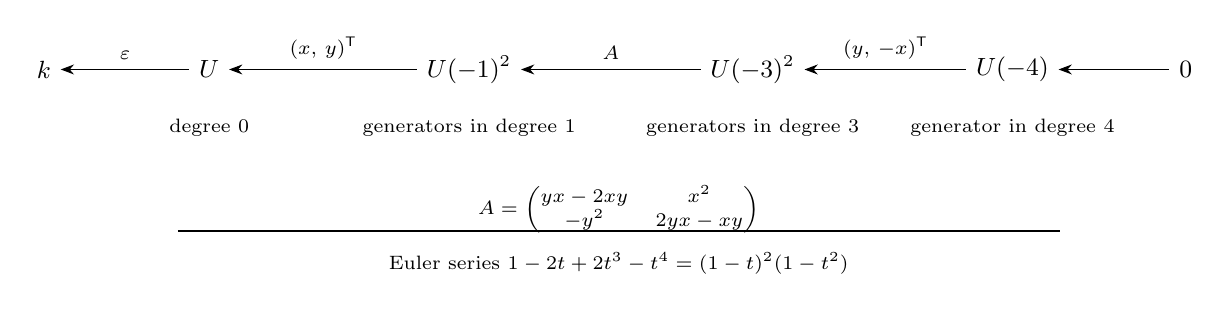
\begin{tikzpicture}[x=1cm,y=1cm,font=\small,>=Stealth]
\node (m0) at (0,0) {$U$};
\node (m1) at (3.3,0) {$U(-1)^2$};
\node (m2) at (6.9,0) {$U(-3)^2$};
\node (m3) at (10.2,0) {$U(-4)$};
\node (m4) at (12.4,0) {$0$};
\node (k) at (-2.1,0) {$k$};
\draw[<-] (k) -- node[above,font=\scriptsize]{$\varepsilon$} (m0);
\draw[<-] (m0) -- node[above,font=\scriptsize]{$(x,\,y)^{\mathsf T}$} (m1);
\draw[<-] (m1) -- node[above,font=\scriptsize]{$A$} (m2);
\draw[<-] (m2) -- node[above,font=\scriptsize]{$(y,\,-x)^{\mathsf T}$} (m3);
\draw[<-] (m3) -- (m4);
\node[font=\scriptsize,anchor=north] at (0,-0.5) {degree $0$};
\node[font=\scriptsize,anchor=north] at (3.3,-0.5) {generators in degree $1$};
\node[font=\scriptsize,anchor=north] at (6.9,-0.5) {generators in degree $3$};
\node[font=\scriptsize,anchor=north] at (10.2,-0.5) {generator in degree $4$};
\node[font=\scriptsize,anchor=north] at (5.2,-1.35) {$A=\begin{pmatrix}yx-2xy&x^2\\-y^2&2yx-xy\end{pmatrix}$};
\draw[thick] (-0.4,-2.05) -- node[below=4pt,font=\scriptsize]{Euler series $1-2t+2t^3-t^4=(1-t)^2(1-t^2)$} (10.8,-2.05);
\end{tikzpicture}

\caption{The resolution of the trivial module over $U$ of Table~\ref{tab:trivial} as a complex of free modules, with the degrees of the generators below each term and the Euler series of the ranks below the complex; the global dimension of $U$ is $3$ and the table is read from left to right.}
\label{fig:resolution}
\end{figure}

\begin{lemma}\label{lem:trivial}
The complex $0\leftarrow U\leftarrow U(-1)^2\leftarrow U(-3)^2\leftarrow U(-4)\leftarrow0$ with maps $(u,v)\mapsto ux+vy$, $(s,t)\mapsto(s,t)A$ with $A=\begin{pmatrix}yx-2xy&x^2\\-y^2&2yx-xy\end{pmatrix}$, and $w\mapsto w(y,-x)$ is a resolution of the left trivial module. The anti-automorphism $\tau$ turns it into a resolution of $k_U$ whose last map is $w\mapsto(yw,-xw)$, and for every left module $M$
\begin{equation}\label{eq:tor3}
\Tor_3^U(k_U,M)\cong\{m\in M: xm=0=ym\}(-4)=\operatorname{soc}(M)(-4).
\end{equation}
\end{lemma}
\begin{proof}
The Chevalley--Eilenberg complex of $H$ is a free resolution of $k$ and cancels to this minimal complex~\cite[Section~6]{ES16}. We check that the composites vanish: $y(yx-2xy)+xy^2=-r_2=0$ and $yx^2-x(2yx-xy)=r_1=0$ in $U$. The two identities are confirmed in the PBW basis by exact computation (Section~\ref{sec:expdesign}) [MV]. The anti-automorphism $\tau$ fixes $r_1$ and $r_2$, so it maps the complex to a complex of right free modules with the last map $w\mapsto(yw,-xw)$. Tensoring this complex with $M$ and reading the last term gives $\Tor_3=\ker(M\to M^2,\ m\mapsto(ym,-xm))$ shifted by $4$, which is~\eqref{eq:tor3}; no finiteness of $M$ is used.
\end{proof}

\subsection{Pure rays, primitive points and the parity test}
\label{sec:parity}

A degree sequence is $d=(0,d_1,d_2,d_3)$ with $0<d_1<d_2<d_3$; a shift of degrees changes nothing, so the invariant is $d_3-d_0$ and we take $d_0=0$. The Betti table of a finite length module over $S$ with a pure resolution of type $d$ satisfies the Herzog--K\"uhl equations
\begin{equation}\label{eq:HK}
\sum_{i=0}^{3}(-1)^i\beta_id_i^m=0\quad(m=0,1,2),\qquad\text{so}\qquad \beta_i\ \propto\ \prod_{j\ne i}\frac1{|d_j-d_i|},
\end{equation}
one equation for each of the first three coefficients of the Hilbert polynomial~\cite{HK84,ES09}. The solution space is a ray; its least integral point is the primitive point $\beta_d$, and every integral point is $m\beta_d$ with $m\ge1$. For $d=(0,e,3e,4e)$ the ratios are $1/(12e^3):1/(6e^3):1/(6e^3):1/(12e^3)$ and $\beta_d=(1,2,2,1)$. Put $p_\beta(t)=\sum_i(-1)^i\beta_it^{d_i}$.

\begin{lemma}[Hilbert series over $S$ and over $U$]\label{lem:parity}
A finitely generated graded $S$-module with Betti table $\beta$ has Hilbert series $p_\beta(t)/(1-t)^3$; a finitely generated graded $U$-module with Betti table $\beta$ has Hilbert series $p_\beta(t)/((1-t)^2(1-t^2))$. A finite length $U$-module with a pure table of type $d$ therefore has $p_\beta(-1)=0$.
\end{lemma}
\begin{proof}
The alternating sum over the minimal free resolution of the Hilbert series of the free modules gives the formulas, with~\eqref{eq:HSU} for $U$. A finite length module has a polynomial Hilbert series; since $(1-t)^2(1-t^2)=(1-t)^3(1+t)$ the numerator $p_\beta$ is divisible by $1+t$, hence $p_\beta(-1)=0$.
\end{proof}

The parity value $p_\beta(-1)$ is homogeneous of degree one in $\beta$, so the test is a property of the ray: it excludes every multiple of $\beta_d$ at once or none. It is the numerical test of Jiang, Li, Sun, Wang, Xiao and Yu~\cite{JLSWXY}. Over $S$ the other standard restriction is Krull's: a cyclic module $S/I$ with $I$ generated by two forms has Krull dimension at least $1$, because every minimal prime of $I$ has height at most $2$; so $\beta_0=1$ and $\beta_1=2$ are impossible for finite length, whatever the degrees (Lemma~\ref{lem:krull} below uses the same argument for $a$ generators).

\subsection{Realizability, scaling, duality and direct sums}
\label{sec:realizability}

\begin{definition}
A point $\beta$ is \emph{realized} over $S$ (respectively $U$) over $k$ if some finite length graded module over $S\otimes k$ (respectively $U\otimes k$) has Betti table $\beta$; it is \emph{excluded} when no such module exists and \emph{open} when neither is known. For a ray and a field $k$, $c_d(k)$ is the least $m\ge1$ such that $m\beta_d$ is realized over $S\otimes k$ (Erman, question~(2) of Section~7~\cite{Erman09}); unless stated otherwise $k$ has characteristic $0$.
\end{definition}

Four elementary facts are used. First, direct sums: if $\beta$ and $\beta'$ are realized on the same ray over the same ring, so is $\beta+\beta'$; hence if the primitive point is realized, every integral point of the ray is. Second, scaling over $S$: if $(d,\beta)$ is realized over $S$ then so is $(ed,\beta)$ for every $e\ge1$. Indeed, let $S'=k[u,v,w]$ with the three generators in degree $e$ and let $S'\to S$ send $u,v,w$ to $x^e,y^e,z^e$; $S$ is free over $S'$ on the monomials with exponents below $e$, so the map is flat, a minimal resolution over $S'$ base-changes to a minimal resolution over $S$ with the twists multiplied by $e$ and the ranks unchanged, and the module has finite length since $S$ is finite over $S'$ [D]. Third, duality over $S$: for a finite length module $M$ with a pure resolution $F$, the complex $\operatorname{Hom}(F,S)$ is exact except at the end and resolves $\Ext^3_S(M,S)$ with the reversed table and the degree sequence $(0,d_3-d_2,d_3-d_1,d_3)$ [D, standard; Erman~\cite[Remark~3.2]{Erman09}]. Fourth, over $U$ we use neither scaling nor duality for any claim: the computation over $U$ archived as \EXP{002} tests the reversal of tables on \ndualCases{} random finite length modules, and the result is evidence only.

\subsection{Pairs of forms, the Hilbert function and the locus of pure pairs}
\label{sec:pairsetting}

A module over $U$ with the table $(1,2,2,1)$ on $(0,e,3e,4e)$ has $\beta_0=1$ and $\beta_1=2$ with the relations in degree $e$, so it is cyclic and equals $U/UW$ for a two-dimensional subspace $W\subset U_e$. Let $u(n)=\dim_kU_n$, which by~\eqref{eq:HSU} is $\lfloor(n+2)^2/4\rfloor$ for $n\ge0$; we put $u(n)=0$ for $n<0$, which the formula alone does not give. For $e\ge2$ let $G_e=\operatorname{Gr}(2,U_e)$, a smooth irreducible variety of dimension $2(u(e)-2)$, and for $W\in G_e$ put $M_W=U/UW$. Left multiplication
\begin{equation}\label{eq:mu}
\mu_n(W):U_{n-e}\otimes W\longrightarrow U_n
\end{equation}
has image $(UW)_n$, so $\dim(M_W)_n=u(n)-\operatorname{rank}\mu_n(W)$. Call $W$ \emph{pure} when $M_W$ has the table $(1,2,2,1)$ on $(0,e,3e,4e)$, and let $P_e\subset G_e$ be the set of pure spaces. By Lemma~\ref{lem:parity} a pure $W$ has the Hilbert function
\begin{equation}\label{eq:hen}
h_e(n)=u(n)-2u(n-e)+2u(n-3e)-u(n-4e),
\end{equation}
the coefficient of $t^n$ in $h_e(t)$ of~\eqref{eq:he}; it vanishes for $n\ge4e-3$ and sums to $e^3$. Two values are used below: $h_e(3e)=u(3e)-2u(2e)+2$ equals $((e-2)/2)^2$ for $e$ even and $(e-1)(e-3)/4$ for $e$ odd, that is $0,0,1,2,4,6$ for $e=2,\dots,7$, and
\begin{equation}\label{eq:fourE}
2u(e)-4-2h_e(3e)=4e-4\qquad\text{for every }e\ge2.
\end{equation}
[MV] The script of the paper checks~\eqref{eq:hen}, these closed forms and~\eqref{eq:fourE} against the Hilbert series of $U$ for $e\le\nformulaMaxE$.

Put $r=2u(2e)-2$. If $W$ is pure, $\mu_n(W)$ is injective for $n<3e$ (the first syzygies of $M_W$ are generated in degree $e$ and the second in degree $3e$) and the kernel of $\mu_{3e}(W)$ has dimension $2$, the two second syzygies, so $\operatorname{rank}\mu_{3e}(W)=r$. Let
\begin{equation}\label{eq:De}
D_e=\{W\in G_e:\ \operatorname{rank}\mu_{3e}(W)\le r\}.
\end{equation}
Then $P_e\subset D_e$. For $e=2,3$ one has $h_e(3e)=0$, so $D_e=G_e$; for $e\ge4$ the maximal-rank function $\max(0,u(n)-2u(n-e))$ and $h_e(n)$ differ exactly in the degrees $3e,\dots,4e-4$, so a pure pair does not have the maximal-rank Hilbert function [MV for $e\le\nformulaMaxE$], and it is special (it lies in the proper closed set $D_e$) whenever some pair has $\operatorname{rank}\mu_{3e}>r$: so for $e=4,5,10$ (Section~\ref{sec:ablation}) and, in characteristic $0$, for $e=4,\dots,7$ (Proposition~\ref{prop:exact}). The graded automorphisms of $U$ are the elements of $\mathrm{GL}_2$ acting on $U_1=\langle x,y\rangle$ with $z\mapsto\det(g)\,z$; they preserve Betti tables and act on $G_e$ through $\mathrm{PGL}_2$, which has dimension $3$. Write $W_0=\langle x^e,y^e\rangle$ and $S_e\subset U_e$ for the span of the $e$-th powers of linear forms $ax+by$; the orbit of $W_0$ consists of the spaces $\langle l_1^e,l_2^e\rangle\subset S_e$. In Sections~\ref{sec:pairsearch} and~\ref{sec:resodd} the forms are printed in the basis of the monomials $x^iy^jz^k$ (the product in this order), which is a basis of $U$ as well because $yx=xy-z$.

\FloatBarrier
\section{Methods}
\label{sec:methods}

\subsection{Exact linear algebra over \texorpdfstring{$U$}{U}}
\label{sec:exactU}

\paragraph{Product.} Elements of $U$ are written in the PBW basis $y^bx^az^c$. Left multiplication by $y$ shifts the exponent of $y$; left multiplication by $x$ uses $xy=yx+z$ and the centrality of $z$,
\[
x\cdot y^bx^az^c=y^bx^{a+1}z^c+b\,y^{b-1}x^az^{c+1},
\]
and the product of two basis monomials is obtained by applying the letters of the left factor from right to left. All coefficients are integers, so the same code runs over $\Q$ (rational numbers), over a prime field $\F_p$ and over $\F_{2^r}$; the characteristic enters only through the arithmetic of the coefficients. Lemma~\ref{lem:normal} below is the closed form of the product that Theorem~A needs, and the script of the manuscript recomputes it from this rule for $a,e\le9$.

\paragraph{Quotient modules.} A finite length module is given by a presentation $U^a/(U F_1+\dots+U F_b)$ with homogeneous $F_j\in(U_{e_j})^a$. Degree by degree, the submodule in degree $d$ is the span of the products $mF_j$ over PBW monomials $m$ of degree $d-e_j$, reduced by exact Gaussian elimination in the field; the dimension of the quotient in degree $d$ is $a\dim U_d$ minus the rank. The matrices of $x$ and $y$ on the quotient in the basis of standard monomials give the module as a graded vector space with the two actions. Algorithm~\ref{alg:module} states the procedure; the module has finite length if the quotient vanishes in consecutive degrees beyond the largest degree of a generator, and the algorithm stops at a stated degree bound otherwise and reports that the module is not known to be finite.

\begin{algorithm}[htbp]
\caption{Quotient of $U^a$ by a left submodule and its Betti table. Input: a field $\Q$, $\F_p$ or $\F_{2^r}$, the generator degrees and the homogeneous relations $F_1,\dots,F_b$, a degree bound $D$. Output: the Hilbert function, the length if finite, the Betti table.}
\label{alg:module}
\begin{algorithmic}[1]
\For{$d=0,1,\dots,D$}
  \State $R_d\gets$ rows $m\,F_j$ for every PBW monomial $m$ of degree $d-e_j$, in the basis of $(U^a)_d$
  \State $\operatorname{rk}_d\gets\operatorname{rank}(R_d)$ by exact elimination; $h_d\gets a\dim U_d-\operatorname{rk}_d$
  \State store the standard monomials of degree $d$ and the reduction map
\EndFor
\If{$h_d=0$ for two consecutive $d\le D$}\State finite length $\sum_dh_d$\Else\State report $h_0,\dots,h_D$ and stop\EndIf
\State build the matrices of $x$ and $y$ on $M_d\to M_{d+1}$
\State $T\gets$ the complex $M\otimes$ (resolution of $k_U$ of Lemma~\ref{lem:trivial}), computed degree by degree
\State $\beta_{i,j}\gets\dim H_i(T)_j$; check $\sum_{i,j}(-1)^i\beta_{i,j}t^j=\Hilb_M(t)\,(1-t)^2(1-t^2)$
\State \Return Hilbert function, length, table
\end{algorithmic}
\end{algorithm}

\subsection{Betti numbers through the resolution of the trivial module, and the second system}
\label{sec:tor}

The Betti numbers are the homology of the complex $K=M\otimes_U(\text{resolution of }k_U)$ of Lemma~\ref{lem:trivial}, whose terms are $M$, $M(-1)^2$, $M(-3)^2$ and $M(-4)$. The complex is checked to be a complex (the composite maps are zero) and exact in degrees $0,\dots,10$ on the calibration modules by rank counts. The Betti table is then read from the ranks. As a second instrument, independent of the first in code and in algorithm, Singular 4.3.2 (Plural) resolves the same module presented over the Heisenberg algebra with the weight ordering $(1,1,2)$; the degree of each generator of each syzygy module gives the Betti table, the function \texttt{betti} of Singular being unreliable on algebras of this type~\cite{Singular}. A table is accepted only when both instruments agree, and for infinite modules the comparison is through the Hilbert function recomputed from the Singular table. The two instruments see the module through different data: the library works with the vector space and the matrices of $x$ and $y$, and Singular with a Gr\"obner basis of the relations, so a convention error shared by both (the sign of $z$, for example) would already fail on the trivial module and on the Kostant modules, whose tables are known in advance.

\subsection{The census over \texorpdfstring{$S$}{S}}
\label{sec:census}

For each of the \nrays{} degree sequences with $d_3\le12$ the census computes, in exact rational arithmetic, the primitive point $\beta_d$ from~\eqref{eq:HK}, the parity value, and the Hilbert functions over $S$ and over $U$. It evaluates the numbers of generators of the three formula constructions (Eisenbud--Schreyer, the two Eisenbud--Fl{\o}ystad--Weyman constructions through the hook-content formula, and S\"oderberg's extremely compressed level modules) and of the standard families, and from them the multiples $m$ for which a construction hits $m\beta_d$. It evaluates six obstructions at every multiple $m\le12$ of the primitive point, with $B=m\beta_d$ (O1 the second syzygy bound $d_2\le(B_0+1)d_1$; O2 the codimension bound $B_1\ge B_0+2$ with the Buchsbaum--Rim table in the equality case; O3 the regularity bound $d_3\le(B_0+2)d_1$~\cite[Proposition~3.1]{Erman09}; O4 a cyclic point $(1,n,n,1)$ with $n$ even~\cite{BE77}; O5 a cyclic point with $B_1=3$, which forces $d=(0,a,2a,3a)$ because three generators of an ideal of height $3$ form a regular sequence; O6 the duals of the previous ones under the duality of Section~\ref{sec:realizability}). Both closures, scaling and duality, are applied, and the census checks that no realization contradicts an obstruction. The result for each ray is an interval $[\mathrm{low}_d,\mathrm{up}_d]$ for $c_d$. Algorithm~\ref{alg:census} states the procedure. The obstructions are never applied over $U$, where only the parity test and explicit modules are used.

\begin{algorithm}[htbp]
\caption{Census of one ray. Input: $d=(0,d_1,d_2,d_3)$, the multiple bound $12$. Output: $\beta_d$, the parity value, the interval $[\mathrm{low}_d,\mathrm{up}_d]$ for $c_d$ and the status of the primitive point.}
\label{alg:census}
\begin{algorithmic}[1]
\State $\beta\gets$ primitive solution of~\eqref{eq:HK}; $\pi\gets p_\beta(-1)$
\For{each construction $\kappa$ with a known number of generators $b_\kappa(d)$}
  \If{$\beta_0\mid b_\kappa(d)$}\State record the realization of $m=b_\kappa(d)/\beta_0$ with its field \EndIf
\EndFor
\For{$m=1,\dots,12$ and each obstruction $O_1,\dots,O_6$}\State record every $O_r$ that excludes $m\beta$\EndFor
\State close under direct sums, scaling and duality; stop with an error if a realized point is excluded
\State $\mathrm{low}_d\gets$ least $m$ not excluded; $\mathrm{up}_d\gets$ least realized $m$
\State status $\gets$ realized if $\mathrm{up}_d=1$, excluded if $\mathrm{low}_d>1$, open otherwise
\end{algorithmic}
\end{algorithm}

\subsection{The search and the rechecks}
\label{sec:search}

Over a prime field the search builds two kinds of random module with the generators of the Macaulay2 package~\cite{M2BS}: a generic level module (the submodule generated by $mB_0$ generic elements of $mB_3$ copies of the truncated injective hull, with the Hilbert function of the pure table), and a generic presentation (the cokernel of a generic $mB_0\times mB_1$ matrix of forms of degree $d_1$), over $\F_{32003}$. A cell is a ray, a multiple $m$, a generator and a seed; $m$ runs from $\mathrm{low}_d$ to $\min(\mathrm{up}_d-1,4)$, three seeds per cell, stopping at the first hit; a resolution that exceeds twenty minutes is recorded as a timeout, never as a miss. Algorithm~\ref{alg:search} states the search. A miss proves nothing, since families of level algebras can be reducible and a generic member need not have the pure table; only the obstructions exclude.

\begin{algorithm}[htbp]
\caption{Search on one open ray over $\F_{32003}$. Input: the ray, $\mathrm{low}_d<\mathrm{up}_d$. Output: a hit (an explicit presentation with the pure table $m\beta_d$) or the list of cells tried.}
\label{alg:search}
\begin{algorithmic}[1]
\For{$m=\mathrm{low}_d,\dots,\min(\mathrm{up}_d-1,4)$}
  \For{generator $\in\{$level module, presentation$\}$ and seed $\in\{1,2,3\}$}
    \State build the random module over $\F_{32003}$; resolve with a time limit of twenty minutes
    \If{the Betti table equals $m\beta_d$}\State save the presentation; \Return hit\EndIf
  \EndFor
\EndFor
\State \Return open (a miss proves nothing)
\end{algorithmic}
\end{algorithm}

Every hit is rechecked (Algorithm~\ref{alg:recheck}): in a fresh Macaulay2 process from the saved presentation, in Singular from the same presentation, and over the rationals. The rational module is not the lift of the saved prime-field presentation: for a generic presentation it is the cokernel of the generator matrix lifted to symmetric integer representatives, and for a level module it is the image of the lifted generator matrix inside the truncated ring. The lift of the presentation computed over $\F_{32003}$ for a level module is not pure in a control we ran (Section~\ref{sec:ablation}; an unarchived control [U]), so the rational module is a new module that realizes the point over $\Q$ if and only if its own resolution over $\Q$ is pure with the right numbers; the reduction modulo $32003$ plays no logical role, and a hit without a completed positive rational recheck stays a realization over $\F_{32003}$ until the rank certificate of Section~\ref{sec:rank} decides it (Section~\ref{sec:lift-results}).

\begin{algorithm}[htbp]
\caption{Recheck of one hit. Input: a saved hit (generator matrix over $\F_{32003}$, ray, multiple, generator type). Output: three results on the pure table, and the rational module with its table.}
\label{alg:recheck}
\begin{algorithmic}[1]
\State resolve the saved presentation in a fresh Macaulay2 process; compare with $m\beta_d$
\State resolve the same presentation in Singular (\texttt{mres}); compare
\State lift the generator matrix to symmetric integer representatives modulo $32003$
\If{generic presentation}\State $P\gets$ cokernel of the lifted $mB_0\times mB_1$ matrix over $\Q[x,y,z]$
\Else\State $P\gets$ image of the lifted matrix in $(\Q[x,y,z]/(x^{r+1},y^{r+1},z^{r+1}))^{mB_3}$ with $r=d_3-3$
\EndIf
\State resolve $P$ over $\Q$ in Macaulay2 with a time limit of thirty minutes; classify: pure, not pure, time limit
\end{algorithmic}
\end{algorithm}

\subsection{The rank certificate of a lift}
\label{sec:rank}

A resolution over $\Q$ is expensive, and a run that ends without a result says nothing, as Section~\ref{sec:lift-results} shows. Proposition~\ref{prop:lift} replaces it by a cheaper exact test on the same lifted module: for each degree $d$ build the integer matrix $A_d$ that defines the graded piece of the lifted module, from the saved generator matrix lifted to symmetric integer representatives, and compare its rank over $\Q$ with its rank over $\F_{32003}$. On every hit the rank over $\F_{32003}$ is maximal in every degree the proposition needs, and since the rank over $\Q$ of an integer matrix is at least its rank modulo $p$, this forces equal ranks; the rational ranks computed by two instruments are a cross-check. For a generic presentation (the cokernel form) $A_d$ has one row for each basis element of the target in degree $d$ and one column for each product of a monomial with a relation; for a level module (the image form) it is the matrix of the generator matrix between the corresponding pieces of the truncated ring $T$. Algorithm~\ref{alg:rank} states the procedure. Two instruments compute the ranks independently: python-flint on integer matrices (\texttt{fmpz\_mat.rank} over $\Q$, \texttt{nmod\_mat.rank} modulo $32003$), and PARI/GP (\texttt{matrank} on the same integer matrix and on its reduction) on every matrix of at most $2{,}000$ rows and on a sample of larger ones.

\begin{algorithm}[htbp]
\caption{Rank certificate for one hit. Input: a saved hit over $\F_{32003}$ with its pure table $m\beta_d$ and its generator matrix. Output: pass, fail or undecided, with the list of degrees where the ranks differ.}
\label{alg:rank}
\begin{algorithmic}[1]
\State lift the generator matrix to symmetric integer representatives
\For{each degree $d$ from $0$ to the top degree plus one of the module over $\F_{32003}$}
  \State build the integer matrix $A_d$ of the cokernel form or of the image form
  \State $r_p\gets\operatorname{rank}_{\F_{32003}}(A_d)$; check that $\operatorname{rows}(A_d)-r_p$ (cokernel form) or $r_p$ (image form) equals the pure Hilbert function in degree $d$
  \State $r_\Q\gets\operatorname{rank}_\Q(A_d)$ with a limit of twenty minutes; if the limit is reached, mark $d$ undecided
\EndFor
\If{$r_\Q=r_p$ in every degree}\State \Return pass: by Proposition~\ref{prop:lift} the lifted module has the pure table over $\Q$
\ElsIf{$r_\Q>r_p$ in some degree}\State \Return fail (the lift is not flat at $32003$; nothing is said about the ray)
\Else\State \Return undecided\EndIf
\end{algorithmic}
\end{algorithm}

\subsection{The search for pure pairs of forms over small fields}
\label{sec:pairsearch}

A pure pair is searched as a point of $G_e$ over a finite field, in the order that the structure of Section~\ref{sec:pairsetting} dictates: the rank of $\mu_{3e}(W)$ first, then the Hilbert function, then the Betti table. The rank is the cheapest test, and for $e=4,5$ the one that fails on a dense open set of $G_e$ (random spaces with $\operatorname{rank}\mu_{3e}>r$ occur over every field searched and over $\F_{32003}$): a matrix of size $2u(2e)\times u(3e)$ ($50\times49$ at $e=4$, $72\times72$ at $e=5$, $98\times100$ at $e=6$) must have rank $r$ and not its maximal value. Only when $\operatorname{rank}\mu_{3e}(W)\le r$ is the Hilbert function computed, degree by degree to $4e-2$ (the module vanishes from degree $4e-3$ on for the pure function, and a function that does not vanish there is not pure), and only when it equals $h_e$ is the Betti table computed by the Tor complex of Section~\ref{sec:tor}. A pair is accepted as pure when the table is $(1,2,2,1)$ on $(0,e,3e,4e)$ in the exact library and, on a fixed sample of the pure spaces found, in Singular with a script generated from the stored basis by code that shares no arithmetic with the library. The Hilbert function does not certify purity: spaces with the pure Hilbert function and a table with a cancelling pair of Betti numbers occur (Section~\ref{sec:resodd}), which is why the last test is not skipped. Algorithm~\ref{alg:pairs} states the procedure.

\begin{algorithm}[htbp]
\caption{Search for pure pairs over $\F_q$. Input: $e$, a finite field $\F_q$, a list of spaces $W\subset U_e$ (all of them, or random draws with seeds $20261120+$ the index in the family and field, possibly stopped once $40$ pure spaces are found), $r=2u(2e)-2$. Output: the counts by rank of $\mu_{3e}$, by Hilbert function and by Betti table, and the pure spaces with their bases.}
\label{alg:pairs}
\begin{algorithmic}[1]
\For{each space $W=\langle f,g\rangle$ of the list}
  \State $\rho\gets\operatorname{rank}\mu_{3e}(W)$ over $\F_q$ by exact elimination; record $\rho$ in the histogram
  \If{$\rho>r$}\State \textbf{continue}\EndIf
  \State $H\gets$ the Hilbert function $u(n)-\operatorname{rank}\mu_n(W)$ for $n=0,\dots,4e-2$
  \If{$H\ne h_e$}\State record $H$; \textbf{continue}\EndIf
  \State $\beta\gets$ the Betti table by the Tor complex of Section~\ref{sec:tor}
  \If{$\beta$ is $(1,2,2,1)$ on $(0,e,3e,4e)$}\State store $W$ with its basis and seed; test whether $W$ lies in the orbit of $\langle x^e,y^e\rangle$\Else\State record $\beta$ as a table with a cancelling pair\EndIf
\EndFor
\end{algorithmic}
\end{algorithm}

The families are fixed before the run (Section~\ref{sec:expdesign}): at $e=3$ all $\nsixAOneThreeSpaces$ two-dimensional subspaces of $U_3$ over $\F_3$ (the Gaussian binomial $\binom62_3=11011$, asserted by the script) and $2{,}000$ random spaces over each of $\F_5$, $\F_9$, $\F_{25}$ and $\F_{27}$; at $e=4$, $20{,}000$ random spaces over each of $\F_3$, $\F_5$, $\F_7$, $\F_9$, $\F_{11}$ and $\F_{13}$; at $e=5$, $50{,}000$ random spaces over $\F_3$. A later computation addresses the cases left open: $\neightAFivePlanned$ random quintic spaces over $\F_5$, $\neightBSevenPlanned$ over $\F_7$ and $\neightCThreePlanned$ random sextic spaces over $\F_3$, with the rank filter first, and it stops a family once $\neightEarlyStop$ pure spaces are found, since the question is existence; the number of spaces done is recorded, and every share is stated over it. A random space is the row space of a uniformly random $2\times u(e)$ matrix of rank $2$ on the monomial basis. A Betti table over $\F_p$ is the table over every field of characteristic $p$, because $\Tor$ commutes with the extension of the base field, so a pair over $\F_p$ settles the characteristic $p$.

\emph{The orbit test.} A pure $W$ lies in the orbit of $W_0$ exactly when it contains the $e$-th powers of two independent linear forms over the algebraic closure. For the control fields $\F_{11}$ and $\F_{13}$ the test looks for $e$-th powers of linear forms in $W$ over the field and over its quadratic extension, where a pair of conjugate forms is found; the arithmetic is that of the library, and the test is checked on spaces built inside the orbit and outside it. Over the rationals (Section~\ref{sec:resfamily}) the criterion is the dimension of $S_e+W$: a space with $\dim(S_e+W)>\dim S_e$ is outside the orbit over every extension of the field, since $\dim S_e=e+1$ in characteristic $0$ and every space of the orbit lies in $S_e$.

\subsection{The tangent space of the rank locus at a pure point}
\label{sec:tangentmethods}

Let $A=\mu_{3e}(W_0)$ be the matrix with $2u(2e)$ rows (the products $m\,w$ for $m$ a PBW monomial of degree $2e$ and $w\in\{x^e,y^e\}$) and $u(3e)$ columns, of rank exactly $r$ at $W_0$. A chart of $G_e$ at $W_0$ is $W=\langle x^e+f,\ y^e+g\rangle$ with $f,g$ in the span of the monomials of degree $e$ other than $x^e$ and $y^e$, which gives $2(u(e)-2)$ coordinates, and then $\mu_{3e}(W)=A+B(f,g)$ with $B$ linear in $(f,g)$. At a matrix of rank exactly $r$ the tangent space of the variety of matrices of rank at most $r$ consists of the directions $X$ with $\lambda(kX)=0$ for every $k$ in the left kernel $K$ of $A$ ($kA=0$, of dimension $2$ at $W_0$) and every linear form $\lambda$ on the target that vanishes on the row space of $A$ (a space of dimension $h_e(3e)$, the cokernel of $A$). The tangent space of $D_e$ at $W_0$ is therefore the kernel of the linear map
\begin{equation}\label{eq:Tmap}
T:(f,g)\longmapsto\big(\lambda(k\,B(f,g))\big)_{k\in K,\ \lambda},
\end{equation}
whose target has dimension $2h_e(3e)=(2u(2e)-r)(u(3e)-r)$. So
\begin{equation}\label{eq:tangentdim}
\dim T_{W_0}D_e=2(u(e)-2)-\operatorname{rank}T\ \ge\ 2(u(e)-2)-2h_e(3e)=4e-4
\end{equation}
by~\eqref{eq:fourE}, with equality if and only if $T$ is onto. Algorithm~\ref{alg:tangent} states the computation, exact over $\Q$ (fractions) and over a prime field. The routine is tested on the generic determinantal varieties: $3\times4$ matrices of rank at most $2$ at a random matrix of rank $2$ (dimension $10$) and $2\times2$ matrices of rank at most $1$ at a matrix of rank $1$ (dimension $3$), with the chart replaced by all matrices, over $\Q$ and over $\F_{32003}$.

\begin{algorithm}[htbp]
\caption{Tangent space of $D_e$ at $W_0$. Input: $e$ and a field $\Q$ or $\F_p$. Output: $\operatorname{rank}A$, $\dim K$, $\dim\operatorname{coker}A$, $\operatorname{rank}T$ and $\dim T_{W_0}D_e$.}
\label{alg:tangent}
\begin{algorithmic}[1]
\State build $A$ from the products $m\,w$ in the PBW basis; $\rho\gets\operatorname{rank}A$ by exact elimination; check $\rho=2u(2e)-2$
\State $K\gets$ the left kernel of $A$ (basis of dimension $2$); $C\gets$ a basis of the linear forms vanishing on the row space of $A$
\For{each chart coordinate (a monomial of degree $e$ other than $x^e,y^e$, in $f$ or in $g$)}
  \State form $B$ of that coordinate from the products $m\,(\text{monomial})$ and store the column $\big(\lambda(kB)\big)_{k,\lambda}$
\EndFor
\State $\operatorname{rank}T\gets$ the rank of the matrix of these columns; \Return $2(u(e)-2)-\operatorname{rank}T$
\end{algorithmic}
\end{algorithm}

The two directions of the orbit of $W_0$ (the derivatives of $x^e$ under $x\mapsto x+ty$ and of $y^e$ under $y\mapsto y+tx$) must lie in the kernel of $T$, which is checked. The linear family $L_e(a,b,c,d)$ of~\eqref{eq:Le} and the plane section $\langle x^4+\alpha x^2y^2+\beta xyz+\gamma z^2,\ y^4\rangle$ of Section~\ref{sec:resfamily} are tested by the rank of $\mu_{3e}$ on finite sets of parameters, and the spaces whose two forms have a common factor modulo $z$ by the rank and by the Hilbert function.

\subsection{The linear family in odd characteristic below \texorpdfstring{$2e$}{2e}: enumeration and stopping rule}
\label{sec:lfmethods}

The linear family $L_e(a,b,c,d)$ of~\eqref{eq:Le} has $p^4$ members over $\F_p$, so the question whether it holds a pure member in characteristic $p$ is decided by enumeration, in two stages. The first stage computes, for every member, the rank of $\mu_{3e}$ (the matrix of~\eqref{eq:mu} with $n=3e$) by exact elimination and compares it with $r=2u(2e)-2$: a member of rank above $r$ would refute the inclusion $L_e\subset D_e$ in that characteristic, and a member of rank below $r$ is not pure. The second stage takes the members of rank exactly $r$ in the lexicographic order of $(a,b,c,d)$ and computes the Hilbert function to degree $4e+2$ and, when it equals $h_e$, the Betti table by the Tor complex of Section~\ref{sec:tor}. The second stage of a pair $(e,p)$ stops once the tasks that were running when $40$ pure members had been found have finished, so a pair that stops early has examined between $160$ and $240$ members of rank $r$ and reports its pure members among those examined; the first stage is complete for every pair. Algorithm~\ref{alg:lf} states the procedure.

\begin{algorithm}[htbp]
\caption{The linear family over $\F_q$. Input: $e$, a prime power $q=p$ or $p^2$, a list of members $(a,b,c,d)\in\F_q^4$ (all of them over $\F_p$, or $20{,}000$ random ones over $\F_{p^2}$ with seed $20261120+$ the index of the pair), $r=2u(2e)-2$, the cap of $40$ pure members (family over $\F_p$) or $10$ (family over $\F_{p^2}$). Output: the histogram of $\operatorname{rank}\mu_{3e}$, the members above $r$, the pure members with their parameters.}
\label{alg:lf}
\begin{algorithmic}[1]
\For{each member $W=L_e(a,b,c,d)$}
  \State $\rho\gets\operatorname{rank}\mu_{3e}(W)$ by exact elimination; record $\rho$ in the histogram; \textbf{if} $\rho>r$ \textbf{then} record $W$ as a member above $r$
\EndFor
\For{each member of rank $\rho=r$ in the order of the list, until the cap is reached}
  \State $H\gets$ the Hilbert function $u(n)-\operatorname{rank}\mu_n(W)$ for $n=0,\dots,4e+2$
  \If{$H=h_e$}\State $\beta\gets$ the Betti table by the Tor complex; record $W$ as pure if $\beta$ is $(1,2,2,1)$ on $(0,e,3e,4e)$\Else\State record $H$ \EndIf
\EndFor
\State \Return the histogram, the members above $r$, the pure members (the first five of each pair are rechecked in Singular)
\end{algorithmic}
\end{algorithm}

Over $\F_p$ the enumeration covers the fifteen pairs $(e,p)$ with $p$ odd, $p<2e$ and $4\le e\le7$, and five control pairs with $p\ge2e$ where Proposition~\ref{prop:linear} applies: $(4,11)$, $(4,13)$, $(5,11)$, $(5,13)$ and $(6,13)$. Over $\F_{p^2}$ (the family is built by a routine of its own, because the constructor of the earlier computations takes integers) the sample is drawn only for the nine pairs below $2e$ in which the enumeration over $\F_p$ found no pure member. A Betti table over $\F_p$ or $\F_{p^2}$ is the table over every field of characteristic $p$ that contains it, so one pure member settles that characteristic. The fixed order and the early stop mean that counts of pure members in a pair that stopped early are counts among the members examined and not shares of the family.

\subsection{Deciding the criterion by a Gr\"obner basis over \texorpdfstring{$\F_p$}{Fp}}
\label{sec:critmethods}

The class $V_e$ over $\F_p$ is the span of the central monomials $X^iY^jz^l$ of degree $e$ and of the products $(X^iY^jz^l)x$ and $(X^iY^jz^l)y$ with $X^iY^jz^l$ of degree $e-1$, written in the monomial basis of Section~\ref{sec:exactU}. For a pair $(f,g)$ of the class the criterion of Theorem~\ref{thm:crit}(b)(ii) holds exactly when the ideal $(zD,n(f),n(g))$ of $\F_p[X,Y,z]$ is zero dimensional. The three generators are homogeneous for the grading $\deg X=\deg Y=p$, $\deg z=2$, so their common zeros over an algebraic closure form a cone, and the ideal is zero dimensional exactly when the cone is the origin. A Gr\"obner basis in the graded reverse lexicographic order decides it: the ideal is zero dimensional if and only if the leading monomials of the basis include a pure power of each of $X$, $Y$ and $z$. Algorithm~\ref{alg:crit} states the decision; for each pair of the class the identity $gf-fg=-Dz$, the Hilbert function and, on a fixed sample, the Betti table are computed independently of it, so that the criterion is compared with purity and not assumed.

\begin{algorithm}[htbp]
\caption{The criterion of Theorem~\ref{thm:crit} for a pair of $V_e$ over $\F_p$. Input: $p$, $e$ and the data $(A,\beta_1,\beta_2;B,\delta_1,\delta_2)$ of $f$ and $g$ as polynomials in $X,Y,z$. Output: true if $M=U/(Uf+Ug)$ has finite length (equivalently, the pair is pure), false otherwise.}
\label{alg:crit}
\begin{algorithmic}[1]
\State $D\gets\beta_1\delta_2-\beta_2\delta_1$; $n(f)\gets A^p+\beta_1^pX+\beta_2^pY$; $n(g)\gets B^p+\delta_1^pX+\delta_2^pY$ in $\F_p[X,Y,z]$
\State check in $U$ that $gf-fg=-Dz$ (exact arithmetic in the monomial basis)
\State $G\gets$ a Gr\"obner basis of $(zD,n(f),n(g))$ in graded reverse lexicographic order
\If{the leading monomials of $G$ contain a power of $X$, a power of $Y$ and a power of $z$}\State \Return true\Else\State \Return false\EndIf
\end{algorithmic}
\end{algorithm}

The random pairs of the class are drawn with uniform coefficient vectors on the monomial basis of $V_e$ over $\F_p$, $200$ for each of the eight pairs $(e,p)$ of Table~\ref{tab:critrand}, with seed $20261120$ plus the index of the pair $(e,p)$ in the list of the table counted from $0$. For each random pair the identity, the criterion and the pure Hilbert function are recorded, with the ranks computed until the first degree whose dimension differs from $h_e$; the Betti table is computed for the first ten pairs with the pure Hilbert function of each case.

\subsection{Admissibility of a stratum}
\label{sec:stratamethods}

Whether a stratum $S(m;i,j)$ is admissible for $e$ (Definition~\ref{def:admissible}) is a finite computation: build the table of the numbers $u_k(n)=\sum_{w\equiv k}(\min(w,n-w)+1)$ for $0\le n\le4e+6m+2$ and the $m$ classes $k$, form the array $u_k(n)-u_{k-i}(n-e)-u_{k-j}(n-e)$, and look for classes $s_1\le s_2$ and $t$ such that adding $u_{k-s_1}(n-3e)+u_{k-s_2}(n-3e)-u_{k-t}(n-4e)$ makes every entry nonnegative. The search over $(s_1,s_2,t)$ has $m^2(m+1)/2$ cases, on an array of $m(4e+6m+3)$ entries. The range of $n$ is the one of Definition~\ref{def:admissible}, which makes the finite test equivalent to the condition for every $n$; a stratum is declared not admissible only after all triples have been tried. The same routine, with the witness $(s_1,s_2,t)=(i,j,0)$ supplied, checks that no stratum with $m$ dividing $e$ is excluded for $e\le10$, and the totals for $e=9$ and $e=10$ are recomputed in the same way. The refined list is obtained from the admissible one by testing, for each stratum, every modulus $m'\le e+1$ for which the weights in $[0,e]$ of the class $i$ lie in one class modulo $m'$ and those of the class $j$ in one class: the stratum is refined admissible when every such $S(m';i',j')$ is admissible. Algorithm~\ref{alg:strata} states the procedure. The script checks the resulting numbers for $e=4,\dots,8$ against an independent computation made earlier (Table~\ref{tab:stratatot}).

\begin{algorithm}[htbp]
\caption{Admissible and refined admissible strata of degree $e$. Input: $e\ge4$. Output: the admissible strata $(m,i,j)$ with $2\le m\le e+1$, $0\le i\le j<m$, and the refined admissible ones.}
\label{alg:strata}
\begin{algorithmic}[1]
\For{$m=2,\dots,e+1$ and $0\le i\le j<m$}
  \State $B_k(n)\gets u_k(n)-u_{k-i}(n-e)-u_{k-j}(n-e)$ for $0\le n\le4e+6m+2$ and $k$ modulo $m$
  \State admissible$(m,i,j)\gets$ \textbf{true} if some $s_1\le s_2$ and $t$ make $B_k(n)+u_{k-s_1}(n-3e)+u_{k-s_2}(n-3e)-u_{k-t}(n-4e)\ge0$ for all $k,n$
\EndFor
\For{each stratum $(m,i,j)$ that is admissible}
  \For{$m'=2,\dots,e+1$ with $m'\ne m$}
    \State $I\gets\{w\bmod m':0\le w\le e,\ w\equiv i\ (m)\}$; $J\gets\{w\bmod m':0\le w\le e,\ w\equiv j\ (m)\}$
    \If{$|I|=|J|=1$ and the stratum $(m';I,J)$ is not admissible}\State mark $(m,i,j)$ as not refined admissible\EndIf
  \EndFor
\EndFor
\end{algorithmic}
\end{algorithm}

\subsection{Searches in the weight-class strata and in the middle stratum}
\label{sec:strsearch}

A stratum $S(m;i,j)$ with $i<j$ has $N=\frac{p^{d_i}-1}{p-1}\cdot\frac{p^{d_j}-1}{p-1}$ members over $\F_p$ (the pairs $(f,g)$ of coefficient vectors on the two supports, each normalized so that its first nonzero coefficient in the order of the library is $1$), where $d_i$ is the number of monomials of degree $e$ and class $i$; a stratum with $i=j$ has one support and its members are only sampled, and a stratum with $d_i<2$ is empty. For a stratum with budget $B$ all $N$ members are taken when $i<j$ and $N\le B$, otherwise $B$ random members (uniform coefficient vectors on the supports). For every member the rank of $\mu_{3e}$ is computed; when it equals $r$ the remaining ranks of the pure Hilbert function are computed, stopping at the first that fails ($\mu_{3e-1}$ injective and $\operatorname{rank}\mu_n=u(n)-h_e(n)$ for $n=3e+1,\dots,4e-3$, which give the Hilbert function $h_e$ in every degree because a kernel element of $\mu_n$ with $n\le3e-2$ would give at least $u(2)=4$ independent kernel elements in degree $3e$, and $I_n=U_n$ at $n=4e-3$ gives $I_n=U_n$ above it); for the members with the pure Hilbert function, in the order found, the Betti table, until $5$ pure members are found or $40$ tables are computed in that stratum. A stratum stops once it has $5$ pure members (the chunks already started finish), so the enumeration of a stratum can be cut: a stratum enumerated in order and stopped early is not a complete enumeration. The matrices of $\mu_n$ are assembled from the structure constants of the product of the library reduced modulo $p$ and their ranks computed with python-flint; the Betti tables use the module construction and the Tor complex of Section~\ref{sec:tor}, and Singular confirms the pure table on the first two pure members of each stratum that has one (at most ten per pair). Three families are searched. Family C: controls on settled pairs, every stratum with $2\le m\le e+1$ (budget $20{,}000$ for an admissible stratum and $3{,}000$ for one that is not). Family Q: the five pairs $(6,5)$, $(6,7)$, $(7,3)$, $(7,5)$, $(7,7)$, every admissible stratum, with the budget $\max(20{,}000,\,30p^{h_e(3e)})$. Family E, exploratory at $e=8$: the three strata $S(2;\cdot)$ at $(8,3)$ with budget $600{,}000$ and every other admissible stratum with $3\le m\le7$ with $100{,}000$; the strata $S(5;0,3)$, $S(6;0,2)$, $S(6;0,4)$, $S(6;2,4)$, $S(7;0,1)$ at $(8,5)$ and $(8,7)$ with $2{,}000{,}000$; the stratum $S(7;0,1)$, which contains the linear family, at $(8,11)$ and $(8,13)$. The middle stratum $S(e;0,e/2)$ (even $e$) and the odd-$e$ strata of the second search are described in Section~\ref{sec:resmid}; the budgets there are $500{,}000$ at $e=8$, $300{,}000$ at $e=10$ and $150{,}000$ at $e=12$ for the stratum $S(e;0,e/2)$, $300{,}000$ for $S(5;0,4)$ at $e=9$, and all members of $S(8;0,1)$ at $e=9$.

\subsection{Pull-backs along an endomorphism}
\label{sec:pbmethods}

For a case of Theorem~\ref{thm:scale} the endomorphism $\varphi$ is given by the polynomials $\varphi(x)$, $\varphi(y)$, $\varphi(z)=\varphi(x)\varphi(y)-\varphi(y)\varphi(x)$; the generators of the module $M'$ are substituted monomial by monomial, $\varphi(x^ay^bz^c)=\varphi(x)^a\varphi(y)^b\varphi(z)^c$, in the product of the library. The Betti table and the length of $M'$ and of $\varphi^*M'=U/(\text{the substituted rows})$ are computed by the library and by Singular and the table of the pull-back is compared with the table of $M'$ with every degree multiplied by $d$; the length is compared with $d^3$ times the length of $M'$. The script of the paper repeats the substitution in its own arithmetic and compares the result with the stored generators. The cases are of two kinds: pure pairs, for which the pull-back is a pure pair of degree $de'$ whose length is $(de')^3$, and modules with other tables, which test that the statement does not depend on the shape $(1,2,2,1)$. Two cases outside the hypotheses, a substitution with $\varphi(z)=0$ and a substitution whose commutator is not central, are computed as controls and no outcome is predicted for the second.

\subsection{Costs}
\label{sec:costs}

Table~\ref{tab:procedures} gives the measured cost of each procedure, read from the records of the computations. The rational computations over $U$ are cheap (the module $M_8$ of length $512$ over $\Q$ takes \nfamilySecondsMax{} seconds), the Singular resolutions of the calibration modules take at most \ncalibMaxTwo{} seconds against \ncalibMaxOne{} seconds for the exact library, and the search is dominated by the long resolutions of a few cells: \ncellsTotal{} cells, of which \ncellsMain{} over $\F_{32003}$ and \ncellsOneE{} characteristic flags over $\F_2$, $\F_3$ and $\F_5$, took \ncellSecondsTotal{} seconds of summed process time with a median of \ncellSecondsMedian{} seconds and a maximum of \ncellSecondsMax{} seconds, in \nsearchWallMin{} minutes of wall time on parallel processes. The census itself was not timed separately; the cost of the programme is that of the search and of the rational rechecks, the latter bounded by a thirty minute limit per hit, and the cost of a hit is dominated by the resolution of the module over $\Q$ and not by the generation of the random matrix.

\begin{table}[htbp]
\centering\footnotesize
\begin{tabular}{@{}>{\raggedright\arraybackslash}p{5.6cm}>{\raggedright\arraybackslash}p{2.6cm}>{\raggedright\arraybackslash}p{5.2cm}@{}}
\toprule
procedure & arithmetic & measured cost\\
\midrule
Exact quotient of $U$ by a left ideal, Tor complex (Algorithm~\ref{alg:module}) & $\mathbb{Q}$, $\mathbb{F}_p$, $\mathbb{F}_{2^r}$ & $e=8$ over $\mathbb{Q}$: 12.6 s; calibration modules: at most 0.12 s\\
Resolution in Plural, degrees read from the generators of each syzygy module & same & calibration modules: at most 1.29 s\\
Census (Algorithm~\ref{alg:census}) & $\mathbb{Q}$ & 220 rays; not timed separately\\
Search (Algorithm~\ref{alg:search}) and characteristic flags & $\mathbb{F}_{32003}$; flags $\mathbb{F}_2,\mathbb{F}_3,\mathbb{F}_5$ & 2{,}996 cells, of which 1046 over $\mathbb{F}_{32003}$ (240 hits) and 1950 characteristic flags; 20{,}089 s of summed process time for all of them, median 0.23 s, maximum 364 s, 16 min wall time\\
Rational recheck (Algorithm~\ref{alg:recheck}) & $\mathbb{Q}$ & 64 completed rechecks, 2 runs without a result, 7 stopped at the 30 minute limit\\
Rank certificate of a lift (Algorithm~\ref{alg:rank}) & $\mathbb{Q}$ and $\mathbb{F}_{32003}$ & 130 hits, 1{,}085 s of summed time; largest matrix $2178\times2200$; longest rank over $\mathbb{Q}$ 647 s\\
Characteristic 2 enumerations and searches & $\mathbb{F}_{2^r}$ & 488 s of summed task time in total, 151.5 s wall time\\
Archived checks of the characteristic 2 theorem & $\mathbb{F}_{2^r}$, $\mathbb{F}_{32003}$, $\mathbb{Q}$, $\mathbb{F}_p$ & 1{,}614 presentations and 24 modules; 43 s wall time\\
Search for pure pairs of forms (Algorithm~\ref{alg:pairs}) & $\mathbb{F}_q$, $q\le27$ & 189{,}011 spaces in 12 families and fields, 9{,}524 s of summed process time, 22 min wall time (EXP-006); 537{,}750 spaces in 3 families stopped early, 13{,}751 s, 29 min (EXP-008)\\
Tangent space of the rank locus (Algorithm~\ref{alg:tangent}) & $\mathbb{Q}$, $\mathbb{F}_p$ & all cases of Section~\ref{sec:resfamily}: 84 s wall time\\
Enumeration of the linear family (Algorithm~\ref{alg:lf}) & $\mathbb{F}_p$, $\mathbb{F}_{p^2}$ & 70{,}271 members over $\mathbb{F}_p$ in the fifteen pairs below $2e$ and 180{,}000 over $\mathbb{F}_{p^2}$; 28 min wall time\\
Central pairs of Theorem~\ref{thm:central} & $\mathbb{F}_p$ & 16 cases, both instruments: 68 s wall time\\
Criterion of Theorem~\ref{thm:crit} (Algorithm~\ref{alg:crit}) & $\mathbb{F}_p$ & 11 explicit pairs and 1{,}600 random pairs: 1{,}398 s of summed time for the random families\\
\bottomrule
\end{tabular}

\caption{Procedures of the methods section, the arithmetic domain of each, and the measured cost read from the archived records of the computations; the census was not timed separately and appears without a figure.}
\label{tab:procedures}
\end{table}

\FloatBarrier
\section{Theory}
\label{sec:theory}

\subsection{The modules \texorpdfstring{$U/U(x^e,y^e)$}{U/U(xe,ye)}: statement}
\label{sec:thmA}

For $e\ge1$ put $M_e=U/U(x^e,y^e)$, the quotient by the left ideal generated by $x^e$ and $y^e$, and
\begin{equation}\label{eq:he}
h_e(t)=\frac{1-2t^e+2t^{3e}-t^{4e}}{(1-t)^2(1-t^2)}=(1+t+\dots+t^{e-1})^2\,(1+t^2+\dots+t^{2e-2}).
\end{equation}
The pure ray $(0,e,3e,4e)$ has the primitive point $(1,2,2,1)$ by~\eqref{eq:HK}. Over $S$ this point is excluded for every $e$ and every field, since a cyclic module $S/I$ with $I$ generated by two forms has Krull dimension at least $1$. The case $e=1$ is the trivial module, and the case $e=2$ is derived by hand and confirmed by the computation archived as \EXP{002}: in degrees $2,\dots,5$ the left ideal $U(x^2,y^2)$ has dimensions $\noneIdealDims$, which are the ranks of explicit elements written in the PBW basis, so $M_2$ has the Hilbert function $(1,2,2,2,1)$ when $2$ and $3$ are invertible.

\begin{thmletter}\label{thm:A}
Let $k$ be a field and $e\ge1$. The module $M_e$ has the pure resolution
\[
0\leftarrow U\leftarrow U(-e)^2\leftarrow U(-3e)^2\leftarrow U(-4e)\leftarrow0
\]
(Betti table $(1,2,2,1)$ on $(0,e,3e,4e)$) if and only if $\ch k=0$ or $\ch k\ge 2e$. In that case $M_e$ has Hilbert series $h_e(t)$, length $e^3$, and a one-dimensional socle, sitting in degree $4e-4$ and weight $0$. For every prime $p\le2e-1$ and $\ch k=p$, the module $M_e$ is nonzero in degree $4e-2$ and does not have this resolution.
\end{thmletter}

The proof occupies Sections~\ref{sec:proofA1} and~\ref{sec:proofA2}; it follows the seven steps of normal ordering, the cokernel over $k[z]$, the binomial blocks, their ranks through the dual Jacobi--Trudi identity and the hook-content formula, the count, the socle through the kernel of $y$ and the symmetry $\sigma$, the resolution, and the converse. Each step states the characteristic it needs, and the machine checks that confirm it are named where they apply [MV]. The argument is complete for every $e$; the finite computations are confirmations and not a part of the proof.

\subsection{Proof of Theorem A, steps 1 to 4: the Hilbert series}
\label{sec:proofA1}

\begin{lemma}[Normal ordering]\label{lem:normal}
For all $a,e\ge0$, in $U$ over every ring,
\begin{equation}\label{eq:normal}
x^ay^e=\sum_{j\ge0}j!\binom aj\binom ej\,z^j\,y^{e-j}x^{a-j}.
\end{equation}
\end{lemma}
\begin{proof}
From $xy=yx+z$ and the centrality of $z$ one gets $xy^e=y^ex+e\,zy^{e-1}$ by induction on $e$: $xy^{e+1}=(y^ex+ezy^{e-1})y=y^e(yx+z)+ezy^e$. This is the case $a=1$. Assume the formula for $a$ and multiply on the left by $x$, using $x\,y^{e-j}=y^{e-j}x+(e-j)\,zy^{e-j-1}$. The coefficient of $z^jy^{e-j}x^{a+1-j}$ in the result is $j!\binom aj\binom ej+(j-1)!\binom a{j-1}\binom e{j-1}(e-j+1)$. Since $(e-j+1)\binom e{j-1}=j\binom ej$, this equals $j!\binom ej\big(\binom aj+\binom a{j-1}\big)=j!\binom{a+1}j\binom ej$. The coefficients are integers, so the identity holds over $\Z$ and in every characteristic; this is what makes the analysis in characteristic $p$ possible.
\end{proof}

\paragraph{Step 1: $M_e$ is a cokernel over $k[z]$.} Right multiplication by $x^e$ maps the PBW basis into itself, because $x$ is the rightmost letter: $(y^bx^az^c)x^e=y^bx^{a+e}z^c$. So $Ux^e$ is spanned by the monomials with $a\ge e$, and $P=U/Ux^e$ is a free $k[z]$-module, with $z$ acting by left multiplication, on the basis $y^bx^a$ with $0\le a<e$ and $b\ge0$. Let $N$ be the image of $Uy^e$ in $P$. Then $M_e=P/N$, and $N$ is the $k[z]$-span of the classes of $u_{a,b}=y^bx^ay^e$ for $a,b\ge0$. By Lemma~\ref{lem:normal} and the vanishing of the terms with $a-j\ge e$ in $P$, $N$ is the image of the $k[z]$-linear map
\begin{equation}\label{eq:Phi}
\Phi(u_{a,b})=\sum_{\substack{0\le j\le\min(a,e)\\ a-j<e}}j!\binom aj\binom ej\,z^j\,y^{b+e-j}x^{a-j}.
\end{equation}
Every term has $a-j<e$ and $j\le e$, so $\Phi(u_{a,b})=0$ for $a\ge2e$, since then $a-j\ge a-e\ge e$. The weight is preserved because $z$ has weight $0$: a source $u_{a,b}$ of weight $b-a+e$ goes to targets $y^{b'}x^{a'}$ with $b'-a'=b-a+e$. Thus $P$, $N$ and $M_e$ split into blocks indexed by the weight $w$.

\paragraph{Step 2: the blocks are binomial Toeplitz matrices.} In the block of weight $w$ the rows are indexed by $a'\in[\max(0,-w),e-1]$ (with $b'=a'+w$) and the columns by $a\ge\max(0,e-w)$ (with $b=a+w-e$). Putting $j=a-a'$ in~\eqref{eq:Phi}, the entry at $(a',a)$ is $\frac{a!}{a'!}\binom e{a-a'}z^{a-a'}$. The class of $z^{n-a'}y^{a'+w}x^{a'}$ has total degree $2n+w$, and the column $a$, of degree $2a+w$, reaches it after multiplication by $z^{n-a}$. Hence, in every characteristic, the piece of $M_e$ of weight $w$ and degree $2n+w$ has dimension
\begin{equation}\label{eq:dimblock}
\dim(M_e)_{(w,\,2n+w)}=|R_n|-\operatorname{rank}\Big[\tfrac{a!}{a'!}\tbinom e{a-a'}\Big]_{a'\in R_n,\ a\in C_n},
\end{equation}
where $R_n=[\max(0,-w),\min(n,e-1)]$ and $C_n=[\max(0,e-w),n]$.
The entries vanish unless $0\le a-a'\le e$, and $a'\le e-1$, so the columns with $a\ge2e$ are zero. Scaling the row $a'$ by $a'!$ ($a'\le e-1$) and the nonzero columns by $1/a!$ ($a\le2e-1$) turns the numeric matrix into
\begin{equation}\label{eq:T}
T[R_n,C_n]=\Big[\tbinom e{a-a'}\Big].
\end{equation}
The scalings are units exactly when $(2e-1)!$ is a unit of $k$, that is when $\ch k=0$ or $\ch k\ge2e$. Under that hypothesis the Hilbert series is $\Hilb(M_e)(t)=\sum_{w,n}\big(|R_n|-\operatorname{rank}T[R_n,C_n]\big)t^{2n+w}$.

\paragraph{Step 3: the ranks.} The matrix $T$ has a nonzero entry exactly when $0\le a-a'\le e$, so only contiguous blocks occur.
\begin{itemize}
\item $0\le w\le e$ and $n\le e-1$: rows $0,\dots,n$, columns $e-w,\dots,n$. The square block on rows and columns $e-w,\dots,n$ is upper unitriangular (the diagonal entries are $\binom e0=1$ and the entries below the diagonal vanish), so the rank is the number of columns, $n-e+w+1$ (zero when $n<e-w$).
\item $0\le w\le e$ and $n\ge e$: the rows are $0,\dots,e-1$ and the usable columns are $e-w,\dots,\min(n,2e-1)$, in number $\mathcal U=\min(n,2e-1)-e+w+1$. The $k\times k$ block on rows $0,\dots,k-1$ and columns $e-w,\dots,e-w+k-1$, with $k=\min(e,\mathcal U)$, has determinant $\det[e_{c-s+s'}](1^e)$ with $c=e-w$, where $e_m(1^e)=\binom em$ is the elementary symmetric polynomial at $e$ ones. By the dual Jacobi--Trudi identity $s_\lambda=\det[e_{\lambda'_i-i+j}]$ with $\lambda'=(c^k)$, this determinant is the Schur polynomial of the rectangle $\lambda=(k^c)$ with $c=e-w$ rows and $k$ columns evaluated at $e$ ones, that is the number of semistandard tableaux of that shape with entries at most $e$; it is positive because $c\le e$. So the rank is $\min(e,\mathcal U)$.
\item $w=-q$ with $1\le q\le e-1$: the rows start at $q$ and the columns at $e+q$. For $n<e+q$ there is no column. For $n\ge e+q$ the usable columns are $e+q,\dots,\min(n,2e-1)$ and the block on rows $q,\dots,q+k-1$ and columns $e+q,\dots,e+q+k-1$ is lower unitriangular ($\binom ee=1$ on the diagonal, zero above), so the rank is $\min(e-q,\mathcal U)$ with $\mathcal U=\min(n,2e-1)-e-q+1$.
\item $w\ge e$: the columns start at $0$ and the block on rows and columns $0,\dots,\min(n,e-1)$ is upper unitriangular, so the block is surjective and contributes nothing. $w\le-e$: there are no rows.
\end{itemize}
The ranks cannot be larger (the number of rows and of nonzero columns bounds them), so these are the ranks in characteristic $0$. In characteristic $p\ge2e$ the minors above are nonzero as well: the unitriangular ones trivially, and the tableau counts by the hook-content formula $s_{(k^c)}(1^e)=\prod_{\text{cells}}(e+\text{content})/\text{hook}$, in which every factor $e+\text{content}$ lies in $[e-c+1,e+k-1]\subseteq[1,2e-1]$ and every hook length is at most $c+k-1\le2e-1$; so the count is prime to $p$. Steps 2 to 4 therefore hold verbatim when $\ch k=0$ or $\ch k\ge2e$.

\paragraph{Step 4: the count.} Write $q=|w|$ and $n'=n-\max(0,-w)$. By step 3 the dimension of the block of weight $w$ in $z$-degree $n$ is
\begin{equation}\label{eq:Dq}
D_q(n')=\begin{cases}\min(n'+1,\,e-q)&0\le n'\le e-1,\\ \max(0,\,2e-1-q-n')&n'\ge e,\end{cases}
\end{equation}
the same for $w$ and $-w$, and zero for $|w|\ge e$. Its generating function in $s$ is the trapezoid $(1+s+\dots+s^{e-q-1})(1+s+\dots+s^{e-1})$, and the class sits in total degree $2n+w=2n'+q$. Hence
\begin{equation}\label{eq:HSMe}
\Hilb(M_e)(t)=(1+t^2+\dots+t^{2e-2})\sum_{|w|<e}t^{|w|}\big(1+t^2+\dots+t^{2(e-|w|-1)}\big)=h_e(t),
\end{equation}
because the sum over $w$ equals $(1+t+\dots+t^{e-1})^2$: grouping the monomials $t^{a+b}$ with $a,b<e$ by $b-a$ gives, for $|b-a|=q$, the terms $t^q,t^{q+2},\dots,t^{2e-2-q}$, each once per sign. Moreover $(1-t^e)^2(1-t^{2e})=1-2t^e+2t^{3e}-t^{4e}$, which is the first form in~\eqref{eq:he}; in particular $M_e$ has finite length $h_e(1)=e^3$. Figure~\ref{fig:weight} shows the blocks for $e=4$, and Figure~\ref{fig:hilbert} the Hilbert functions and the decomposition by $|w|$.

[MV] The exact computation of Section~\ref{sec:exactU} agrees with~\eqref{eq:dimblock} and~\eqref{eq:Dq}: for each $e\le\nfamilyMaxE$ the rank of every weight block (\nblocksChecked{} blocks in total) equals $D_q(n')$ over $\Q$, the resulting Hilbert function is $h_e$, and the Hilbert functions of the modules computed by the library with exact fractions in the experiments equal $h_e$ for $e=2,\dots,\nfamilyMaxE$ (Table~\ref{tab:blocks}, Table~\ref{tab:family}).

\begin{figure}[htbp]
\centering
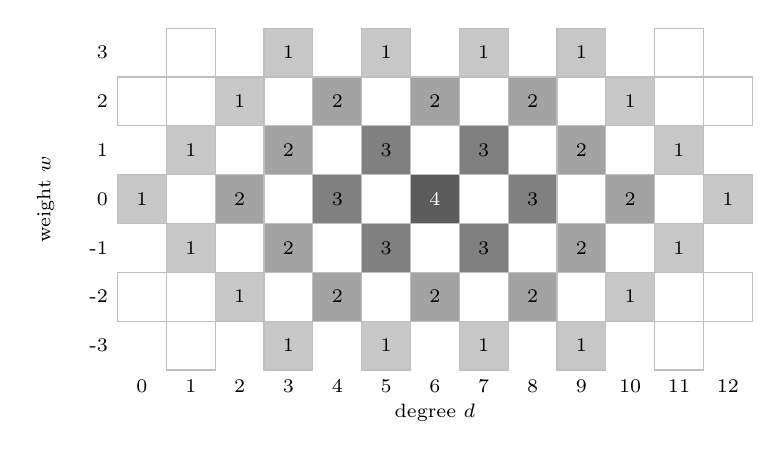
\begin{tikzpicture}[x=0.62cm,y=0.62cm,font=\scriptsize]
\draw[gray!50] (1,0) rectangle +(1,1);
\fill[black!22] (3,0) rectangle +(1,1);
\draw[gray!50] (3,0) rectangle +(1,1);
\node[black] at (3.5,0.5) {1};
\fill[black!22] (5,0) rectangle +(1,1);
\draw[gray!50] (5,0) rectangle +(1,1);
\node[black] at (5.5,0.5) {1};
\fill[black!22] (7,0) rectangle +(1,1);
\draw[gray!50] (7,0) rectangle +(1,1);
\node[black] at (7.5,0.5) {1};
\fill[black!22] (9,0) rectangle +(1,1);
\draw[gray!50] (9,0) rectangle +(1,1);
\node[black] at (9.5,0.5) {1};
\draw[gray!50] (11,0) rectangle +(1,1);
\draw[gray!50] (0,1) rectangle +(1,1);
\fill[black!22] (2,1) rectangle +(1,1);
\draw[gray!50] (2,1) rectangle +(1,1);
\node[black] at (2.5,1.5) {1};
\fill[black!36] (4,1) rectangle +(1,1);
\draw[gray!50] (4,1) rectangle +(1,1);
\node[black] at (4.5,1.5) {2};
\fill[black!36] (6,1) rectangle +(1,1);
\draw[gray!50] (6,1) rectangle +(1,1);
\node[black] at (6.5,1.5) {2};
\fill[black!36] (8,1) rectangle +(1,1);
\draw[gray!50] (8,1) rectangle +(1,1);
\node[black] at (8.5,1.5) {2};
\fill[black!22] (10,1) rectangle +(1,1);
\draw[gray!50] (10,1) rectangle +(1,1);
\node[black] at (10.5,1.5) {1};
\draw[gray!50] (12,1) rectangle +(1,1);
\fill[black!22] (1,2) rectangle +(1,1);
\draw[gray!50] (1,2) rectangle +(1,1);
\node[black] at (1.5,2.5) {1};
\fill[black!36] (3,2) rectangle +(1,1);
\draw[gray!50] (3,2) rectangle +(1,1);
\node[black] at (3.5,2.5) {2};
\fill[black!50] (5,2) rectangle +(1,1);
\draw[gray!50] (5,2) rectangle +(1,1);
\node[black] at (5.5,2.5) {3};
\fill[black!50] (7,2) rectangle +(1,1);
\draw[gray!50] (7,2) rectangle +(1,1);
\node[black] at (7.5,2.5) {3};
\fill[black!36] (9,2) rectangle +(1,1);
\draw[gray!50] (9,2) rectangle +(1,1);
\node[black] at (9.5,2.5) {2};
\fill[black!22] (11,2) rectangle +(1,1);
\draw[gray!50] (11,2) rectangle +(1,1);
\node[black] at (11.5,2.5) {1};
\fill[black!22] (0,3) rectangle +(1,1);
\draw[gray!50] (0,3) rectangle +(1,1);
\node[black] at (0.5,3.5) {1};
\fill[black!36] (2,3) rectangle +(1,1);
\draw[gray!50] (2,3) rectangle +(1,1);
\node[black] at (2.5,3.5) {2};
\fill[black!50] (4,3) rectangle +(1,1);
\draw[gray!50] (4,3) rectangle +(1,1);
\node[black] at (4.5,3.5) {3};
\fill[black!64] (6,3) rectangle +(1,1);
\draw[gray!50] (6,3) rectangle +(1,1);
\node[white] at (6.5,3.5) {4};
\fill[black!50] (8,3) rectangle +(1,1);
\draw[gray!50] (8,3) rectangle +(1,1);
\node[black] at (8.5,3.5) {3};
\fill[black!36] (10,3) rectangle +(1,1);
\draw[gray!50] (10,3) rectangle +(1,1);
\node[black] at (10.5,3.5) {2};
\fill[black!22] (12,3) rectangle +(1,1);
\draw[gray!50] (12,3) rectangle +(1,1);
\node[black] at (12.5,3.5) {1};
\fill[black!22] (1,4) rectangle +(1,1);
\draw[gray!50] (1,4) rectangle +(1,1);
\node[black] at (1.5,4.5) {1};
\fill[black!36] (3,4) rectangle +(1,1);
\draw[gray!50] (3,4) rectangle +(1,1);
\node[black] at (3.5,4.5) {2};
\fill[black!50] (5,4) rectangle +(1,1);
\draw[gray!50] (5,4) rectangle +(1,1);
\node[black] at (5.5,4.5) {3};
\fill[black!50] (7,4) rectangle +(1,1);
\draw[gray!50] (7,4) rectangle +(1,1);
\node[black] at (7.5,4.5) {3};
\fill[black!36] (9,4) rectangle +(1,1);
\draw[gray!50] (9,4) rectangle +(1,1);
\node[black] at (9.5,4.5) {2};
\fill[black!22] (11,4) rectangle +(1,1);
\draw[gray!50] (11,4) rectangle +(1,1);
\node[black] at (11.5,4.5) {1};
\draw[gray!50] (0,5) rectangle +(1,1);
\fill[black!22] (2,5) rectangle +(1,1);
\draw[gray!50] (2,5) rectangle +(1,1);
\node[black] at (2.5,5.5) {1};
\fill[black!36] (4,5) rectangle +(1,1);
\draw[gray!50] (4,5) rectangle +(1,1);
\node[black] at (4.5,5.5) {2};
\fill[black!36] (6,5) rectangle +(1,1);
\draw[gray!50] (6,5) rectangle +(1,1);
\node[black] at (6.5,5.5) {2};
\fill[black!36] (8,5) rectangle +(1,1);
\draw[gray!50] (8,5) rectangle +(1,1);
\node[black] at (8.5,5.5) {2};
\fill[black!22] (10,5) rectangle +(1,1);
\draw[gray!50] (10,5) rectangle +(1,1);
\node[black] at (10.5,5.5) {1};
\draw[gray!50] (12,5) rectangle +(1,1);
\draw[gray!50] (1,6) rectangle +(1,1);
\fill[black!22] (3,6) rectangle +(1,1);
\draw[gray!50] (3,6) rectangle +(1,1);
\node[black] at (3.5,6.5) {1};
\fill[black!22] (5,6) rectangle +(1,1);
\draw[gray!50] (5,6) rectangle +(1,1);
\node[black] at (5.5,6.5) {1};
\fill[black!22] (7,6) rectangle +(1,1);
\draw[gray!50] (7,6) rectangle +(1,1);
\node[black] at (7.5,6.5) {1};
\fill[black!22] (9,6) rectangle +(1,1);
\draw[gray!50] (9,6) rectangle +(1,1);
\node[black] at (9.5,6.5) {1};
\draw[gray!50] (11,6) rectangle +(1,1);
\node[anchor=north] at (0.5,0) {0};
\node[anchor=north] at (1.5,0) {1};
\node[anchor=north] at (2.5,0) {2};
\node[anchor=north] at (3.5,0) {3};
\node[anchor=north] at (4.5,0) {4};
\node[anchor=north] at (5.5,0) {5};
\node[anchor=north] at (6.5,0) {6};
\node[anchor=north] at (7.5,0) {7};
\node[anchor=north] at (8.5,0) {8};
\node[anchor=north] at (9.5,0) {9};
\node[anchor=north] at (10.5,0) {10};
\node[anchor=north] at (11.5,0) {11};
\node[anchor=north] at (12.5,0) {12};
\node[anchor=east] at (0,0.5) {-3};
\node[anchor=east] at (0,1.5) {-2};
\node[anchor=east] at (0,2.5) {-1};
\node[anchor=east] at (0,3.5) {0};
\node[anchor=east] at (0,4.5) {1};
\node[anchor=east] at (0,5.5) {2};
\node[anchor=east] at (0,6.5) {3};
\node[anchor=north] at (6.5,-0.5) {degree $d$};
\node[anchor=south,rotate=90] at (-1.1,3.5) {weight $w$};
\end{tikzpicture}

\caption{The dimension of each piece of $M_4=U/U(x^4,y^4)$ by weight $w$ (rows) and degree $d$ (columns), as computed exactly over $\Q$; the entries are the trapezoids $D_q(n')$ of equation~\eqref{eq:Dq}, with $q=|w|$, and they add up to the length $64=4^3$. Only pieces with $d\equiv w\pmod 2$ can be nonzero, and the shading follows the value.}
\label{fig:weight}
\end{figure}

\begin{figure}[htbp]
\centering
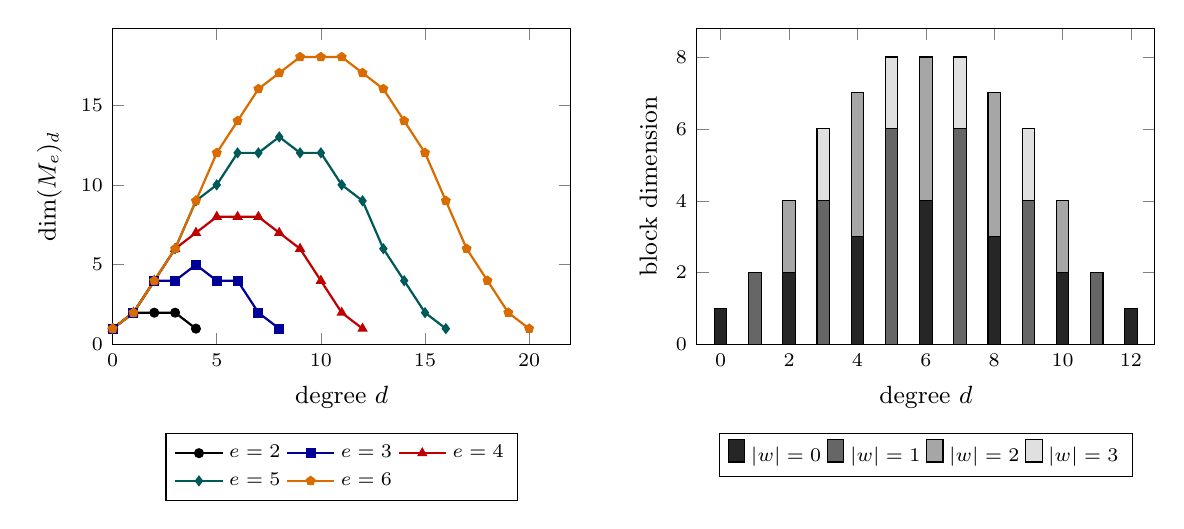
\begin{tikzpicture}
\begin{groupplot}[group style={group size=2 by 1, horizontal sep=1.6cm}, width=7.4cm, height=5.6cm, tick label style={font=\scriptsize}, label style={font=\small}]
\nextgroupplot[xlabel={degree $d$}, ylabel={$\dim (M_e)_d$}, legend style={font=\scriptsize, at={(0.5,-0.28)}, anchor=north}, xmin=0, ymin=0, legend columns=3]
\addplot[color=black, mark=*, mark size=1.4pt, thick] coordinates {(0,1) (1,2) (2,2) (3,2) (4,1)};
\addlegendentry{$e=2$}
\addplot[color=blue!60!black, mark=square*, mark size=1.4pt, thick] coordinates {(0,1) (1,2) (2,4) (3,4) (4,5) (5,4) (6,4) (7,2) (8,1)};
\addlegendentry{$e=3$}
\addplot[color=red!75!black, mark=triangle*, mark size=1.4pt, thick] coordinates {(0,1) (1,2) (2,4) (3,6) (4,7) (5,8) (6,8) (7,8) (8,7) (9,6) (10,4) (11,2) (12,1)};
\addlegendentry{$e=4$}
\addplot[color=teal!70!black, mark=diamond*, mark size=1.4pt, thick] coordinates {(0,1) (1,2) (2,4) (3,6) (4,9) (5,10) (6,12) (7,12) (8,13) (9,12) (10,12) (11,10) (12,9) (13,6) (14,4) (15,2) (16,1)};
\addlegendentry{$e=5$}
\addplot[color=orange!85!black, mark=pentagon*, mark size=1.4pt, thick] coordinates {(0,1) (1,2) (2,4) (3,6) (4,9) (5,12) (6,14) (7,16) (8,17) (9,18) (10,18) (11,18) (12,17) (13,16) (14,14) (15,12) (16,9) (17,6) (18,4) (19,2) (20,1)};
\addlegendentry{$e=6$}
\nextgroupplot[xlabel={degree $d$}, ylabel={block dimension}, ybar stacked, bar width=4.5pt, xmin=-0.7, xmax=12.7, ymin=0, legend style={font=\scriptsize, at={(0.5,-0.28)}, anchor=north}, legend columns=4, xtick distance=2]
\addplot[draw=black, fill=black!85] coordinates {(0,1) (1,0) (2,2) (3,0) (4,3) (5,0) (6,4) (7,0) (8,3) (9,0) (10,2) (11,0) (12,1)};
\addlegendentry{$|w|=0$}
\addplot[draw=black, fill=black!60] coordinates {(0,0) (1,2) (2,0) (3,4) (4,0) (5,6) (6,0) (7,6) (8,0) (9,4) (10,0) (11,2) (12,0)};
\addlegendentry{$|w|=1$}
\addplot[draw=black, fill=black!35] coordinates {(0,0) (1,0) (2,2) (3,0) (4,4) (5,0) (6,4) (7,0) (8,4) (9,0) (10,2) (11,0) (12,0)};
\addlegendentry{$|w|=2$}
\addplot[draw=black, fill=black!12] coordinates {(0,0) (1,0) (2,0) (3,2) (4,0) (5,2) (6,0) (7,2) (8,0) (9,2) (10,0) (11,0) (12,0)};
\addlegendentry{$|w|=3$}
\end{groupplot}
\end{tikzpicture}

\caption{Left: the Hilbert functions of $M_e$ for $e=2,\dots,6$ computed over $\Q$, which equal the coefficients of $h_e(t)$. Right: the Hilbert function of $M_4$ decomposed by $|w|$, each bar being the sum of the blocks of weight $w$ and $-w$ in that degree; the bars stack to $h_4=(1,2,4,6,7,8,8,8,7,6,4,2,1)$.}
\label{fig:hilbert}
\end{figure}

\begin{table}[htbp]
\centering\footnotesize
\begin{tabular}{@{}rrrll@{}}
\toprule
$e$ & blocks $(w,n)$ & primes $p\ge2e$ with generic blocks & primes $p<2e$ (piece in degree $4e-2$) & $\mathbb{Q}$ rank $=D_q$\\
\midrule
2 & 56 & 9 & $\{2,3\}$ & yes\\
3 & 99 & 8 & $\{2,3,5\}$ & yes\\
4 & 154 & 7 & $\{2,3,5,7\}$ & yes\\
5 & 221 & 7 & $\{2,3,5,7\}$ & yes\\
6 & 300 & 6 & $\{2,3,5,7,11\}$ & yes\\
7 & 391 & 5 & $\{2,3,5,7,11,13\}$ & yes\\
8 & 494 & 5 & $\{2,3,5,7,11,13\}$ & yes\\
\bottomrule
\end{tabular}

\caption{Exact check of the proof of Theorem A for $e=2,\dots,8$: the number of weight blocks $(w,n)$ whose dimension was computed from the unscaled matrix of equation~\eqref{eq:dimblock} over $\Q$ and equal to $D_q$; the primes up to $31$ at which all blocks keep the closed form (exactly those with $p\ge2e$); and the primes at which the piece of weight $0$ in degree $4e-2$ is nonzero (exactly those with $p<2e$).}
\label{tab:blocks}
\end{table}

\subsection{Proof of Theorem A, steps 5 to 7: socle, resolution and converse}
\label{sec:proofA2}

\paragraph{Step 5: the socle is one-dimensional.} Assume $\ch k=0$ or $\ch k\ge2e$. Left multiplication by $y$ on $P$ is the shift $y^bx^az^c\mapsto y^{b+1}x^az^c$: it is injective and its image $yP$ is spanned by the basis elements with $b\ge1$.

\emph{The kernel of $y$ on $M_e$.} Let $m\in P$ with $ym\in N$, and write $ym=\sum c_{a,b}(z)\,[y^bx^ay^e]$. The terms with $b\ge1$ are $y$ times an element of $N$. For $b=0$: $x^ay^e$ vanishes in $P$ when $a\ge2e$; for $a<e$ it equals $yg_a$ with $g_a=\sum_{j\le a}j!\binom aj\binom ej z^jy^{e-j-1}x^{a-j}$, because every term of $x^ay^e$ has $y$-exponent $e-j\ge1$; for $e\le a\le2e-1$ its only term with $y$-exponent $0$ is the one with $j=e$, namely $e!\binom ae z^ex^{a-e}=\frac{a!}{(a-e)!}z^ex^{a-e}$, and these terms involve distinct basis elements $x^{a-e}$. Since $ym$ and all the other terms lie in $yP$, comparing the components of $y$-exponent $0$ gives $c_{a,0}(z)\frac{a!}{(a-e)!}z^e=0$ for $e\le a\le2e-1$; the integers $a!/(a-e)!$ are products of factors at most $2e-1$, hence units under the hypothesis, so these coefficients vanish. Injectivity of $y$ on $P$ then gives $m=\nu+\sum_{a<e}c_a(z)g_a$ with $\nu\in N$. Conversely $yg_a=x^ay^e$ lies in $N$. So $\ker(y|M_e)$ is the $k[z]$-span of the classes of $g_0,\dots,g_{e-1}$, and $g_a$ has weight $e-1-a\ge0$. [MV] For $e=2,\dots,\nfamilyMaxE$ over $\Q$ the kernel of $y$ equals the span of the classes $z^cg_a$ in every degree (Table~\ref{tab:family}).

\emph{The symmetry.} The map $\sigma$ of Section~\ref{sec:rings} satisfies $\sigma(x^e)=y^e$ and $\sigma(y^e)=(-1)^ex^e$, so it preserves the left ideal $U(x^e,y^e)$ and induces a $\sigma$-semilinear bijection of $M_e$, $\sigma(um)=\sigma(u)\sigma(m)$. The module $M_e$ is graded by the weight because $x^e$ and $y^e$ are weight-homogeneous; the bijection sends weight $w$ to $-w$ and maps $\ker x$ onto $\ker y$ and $\ker y$ onto $\ker x$. So $\ker x$ lies in the weights $\le0$.

\emph{The socle.} Since $x$ and $y$ are weight-homogeneous, every weight component of a socle element lies in the socle; by the two kernels, the socle lies in weight $0$, inside the weight $0$ part of $\ker y$, which is the cyclic $k[z]$-module generated by the class of $g_{e-1}$ (the summands $k[z][g_a]$ sit in distinct weights). A socle element is also killed by $z=xy-yx$, and the elements of a homogeneous cyclic torsion $k[z]$-module killed by $z$ form a space of dimension at most $1$. So the socle has dimension at most $1$; it is not zero, because $M_e$ is a nonzero module of finite length; and it contains the top degree $4e-4$ of $h_e$, which is one-dimensional. Hence the socle of $M_e$ is $(M_e)_{4e-4}$. [MV] The socle is of weight $0$, degree $4e-4$ and dimension $1$ for $e=2,\dots,\nfamilyMaxE$.

\paragraph{Step 6: the resolution.} By Lemma~\ref{lem:trivial}, $\Tor_3^U(k_U,M_e)=\operatorname{soc}(M_e)(-4)=k(-4e)$ by step 5. $\Tor_0=k$ since $M_e$ is cyclic, and $\Tor_1=k(-e)^2$ since $x^e$ and $y^e$ are minimal generators of the left ideal, which has nothing below degree $e$. By Lemma~\ref{lem:parity} the alternating sum of the Betti series is $\Hilb(M_e)(t)(1-t)^2(1-t^2)=1-2t^e+2t^{3e}-t^{4e}$ by step 4. As $\Tor_0$, $\Tor_1$ and $\Tor_3$ are known exactly and the global dimension is $3$, the Euler identity $1-2t^e+B_2(t)-t^{4e}=1-2t^e+2t^{3e}-t^{4e}$ gives $B_2(t)=2t^{3e}$, where $B_2$ is the Betti series of $\Tor_2$: there is no room for cancellation, and $\Tor_2=k(-3e)^2$. The resolution is pure of type $(0,e,3e,4e)$.

\paragraph{Step 7: the converse.} Let $p\le2e-1$ be a prime (so $e\ge2$) and $\ch k=p$. The integers $e,\dots,2e-1$ contain a multiple $m$ of $p$: if $p\le e$ any $e$ consecutive integers do, and if $e<p\le2e-1$ take $m=p$. Take the block of weight $0$ with $n=2e-1$: the rows are $0,\dots,e-1$ and the columns $e,\dots,2e-1$, an $e\times e$ matrix. The unscaled entries of the column $m$ are $\frac{m!}{a'!}\binom e{m-a'}$ with $a'\le e-1<m$, and $m!/a'!=(a'+1)(a'+2)\cdots m$ contains the factor $m$, so the whole column is $0$ in $k$. The rank is at most $e-1$, and by~\eqref{eq:dimblock}, which is characteristic-free, the piece of weight $0$ and degree $2(2e-1)=4e-2$ is not zero. A module with the resolution of the statement has Hilbert series $h_e$, of degree $4e-4$, so $M_e$ does not have that resolution in characteristic $p$. (The Betti numbers are forced: for a finite length module with a pure resolution of type $(0,e,3e,4e)$ whose table begins $1,2$, the numerator $1-2t^e+b_2t^{3e}-b_3t^{4e}$ vanishes to order at least $2$ at $t=1$, which gives $b_2-b_3=1$ and $3b_2-4b_3=2$, hence $b_2=2$ and $b_3=1$.) Together with steps 2 to 6, $M_e$ has the pure resolution with table $(1,2,2,1)$ if and only if $\ch k=0$ or $\ch k\ge2e$. This proves Theorem~\ref{thm:A}. \qed

[MV] For $e=2,\dots,5$ the primes $p\le23$ at which $M_e$ is not pure over $\F_p$ are exactly $\{2,3\}$, $\{2,3,5\}$, $\{2,3,5,7\}$ and $\{2,3,5,7\}$, the primes below $2e$ (Figure~\ref{fig:primes}); this had been predicted before the computation from the factorials and the tableau counts, which give the same set. For $e=6,7,8$ the exact block computation over $\F_p$ for all primes up to $31$ gives the primes below $2e$ (Table~\ref{tab:blocks}).

\begin{figure}[htbp]
\centering
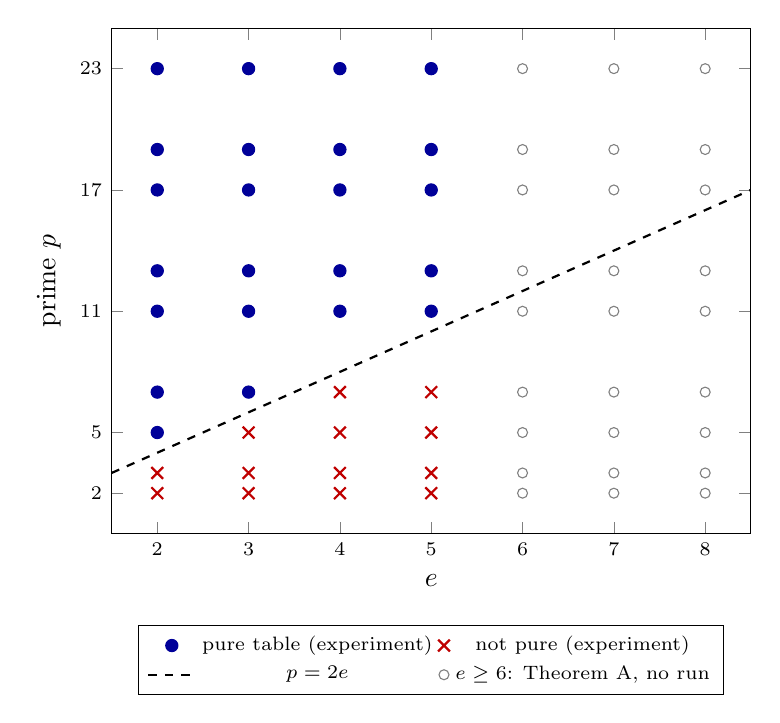
\begin{tikzpicture}
\begin{axis}[width=0.8\textwidth, height=8cm, xlabel={$e$}, ylabel={prime $p$}, xmin=1.5, xmax=8.5, ymin=0, ymax=25, xtick={2,...,8}, ytick={2,5,11,17,23}, tick label style={font=\scriptsize}, legend style={font=\scriptsize, at={(0.5,-0.18)}, anchor=north}, legend columns=2]
\addplot[only marks, mark=*, mark size=2.2pt, color=blue!60!black] coordinates {(2,5) (2,7) (2,11) (2,13) (2,17) (2,19) (2,23) (3,7) (3,11) (3,13) (3,17) (3,19) (3,23) (4,11) (4,13) (4,17) (4,19) (4,23) (5,11) (5,13) (5,17) (5,19) (5,23)};
\addlegendentry{pure table (experiment)}
\addplot[only marks, mark=x, mark size=3pt, thick, color=red!75!black] coordinates {(2,2) (2,3) (3,2) (3,3) (3,5) (4,2) (4,3) (4,5) (4,7) (5,2) (5,3) (5,5) (5,7)};
\addlegendentry{not pure (experiment)}
\addplot[dashed, thick, color=black] coordinates {(1.5,3) (8.5,17)};
\addlegendentry{$p=2e$}
\addplot[only marks, mark=o, mark size=1.8pt, color=gray] coordinates {(6,2) (6,3) (6,5) (6,7) (6,11) (6,13) (6,17) (6,19) (6,23) (7,2) (7,3) (7,5) (7,7) (7,11) (7,13) (7,17) (7,19) (7,23) (8,2) (8,3) (8,5) (8,7) (8,11) (8,13) (8,17) (8,19) (8,23)};
\addlegendentry{$e\ge 6$: Theorem A, no run}
\end{axis}
\end{tikzpicture}

\caption{Characteristics at which $M_e$ has the pure table $(1,2,2,1)$: for $e=2,\dots,5$ and every prime $p\le23$ the experiment gives either the pure table (filled circles) or a module that is not pure (crosses); the dashed line is $p=2e$, which separates the two sets exactly. The light circles and crosses are the primes for $e=6,7,8$ whose status is decided by Theorem~A and by the exact block computation, without a run of the module.}
\label{fig:primes}
\end{figure}

\begin{remark}[{Structure over $k[z]$}]
$M_e$ is not free over $k[z]/(z^e)$. For $e=2$, $M_2\cong k[z]/(z^3)\oplus(k[z]/(z^2))^2(-1)\oplus k[z]/(z)(-2)$, generated by the classes of $1$, $x$, $y$ and $xy-z/2$. For $e\le5$ the experiment finds one summand $k[z]/(z^{2e-1-a-b})$ generated in degree $a+b$ for each pair $a,b<e$, which has the Hilbert series $h_e$. The statement for every $e$ is not derived here and nothing above uses it [MV for $e\le5$, [U] beyond].
\end{remark}

\begin{remark}[{The pair $(x^e,y^e)$ is special for $e\ge4$}]
The series $(1-2t^e)/((1-t)^2(1-t^2))$ of two general forms of degree $e$ has coefficient $-1$ in degree $4e-4$ for $e=4$ (the value is $49-50$, the dimension of $U_{12}$ minus twice that of $U_8$), so the expected (maximal-rank) series vanishes there, while $M_e$ is one-dimensional. For $e=4,5,10$ random pairs over $\F_{32003}$ attain the maximal-rank Hilbert function and are not pure (Section~\ref{sec:ablation}) [MV], so for these $e$ a general pair gives a smaller quotient and the family is realized by a special left ideal. For other $e\ge4$ this is expected and not proved.
\end{remark}

\begin{remark}[{Characteristic $3$ and $e=2$}]\label{rem:charthree}
The pair $(x^2,y^2)$ gives the point exactly for $\ch k=0$ or $\ch k\ge5$. In characteristic $3$ other pairs realize it: random pairs of quadrics over $\F_3$, $\F_9$, $\F_{27}$ and $\F_{81}$ have the table $(1,2,2,1)$ on $(0,2,6,8)$ in \ngfThreeHits, \ngfNineHits, \ngfTwentySevenHits{} and \ngfEightyOneHits{} of $20$ cases (Table~\ref{tab:pairs}) [MV]; the table is stable under extension of the field, so a pair over $\F_q$ gives one over every field of characteristic $3$ containing $\F_q$.
\end{remark}

\subsection{Characteristic \texorpdfstring{$2$}{2} for pairs of quadrics: the elementary argument}
\label{sec:thmB}

\begin{thmletter}\label{thm:B}
Let $k$ be a field of characteristic $2$. No finite length graded module over $U$ has the Betti table $(1,2,2,1)$ on $(0,2,6,8)$. Over $S$, over every field and for every $e$, no finite length module has the table $(1,2,2,1)$ on $(0,e,3e,4e)$.
\end{thmletter}
\begin{proof}
\emph{Step 1: the centre.} In characteristic $2$, $x^2y-yx^2=2xz=0$ and $y^2x-xy^2=-2yz=0$, so $X=x^2$, $Y=y^2$ and $Z=z$ are central. The monomials $y^{2j}x^{2i}z^c$ are distinct PBW basis elements, so $C=k[X,Y,Z]$ is a polynomial ring in three generators of degree $2$, and $y^{2j+\beta}x^{2i+\alpha}z^c=(y^{2j}x^{2i}z^c)\,y^\beta x^\alpha$ shows that $U$ is free over $C$ on $1,x,y,yx$ (equivalently $1,x,y,xy=yx+z$). Hence $U_2=C_2\oplus k\,xy$, of dimension $4=3+1$.

\emph{Step 2: two quadrics always contain a central one.} A two-dimensional subspace $V\subset U_2$ meets $C_2$ in dimension at least $1$: either $V\subset C_2$ or $V=\operatorname{span}(c,f)$ with $c\in C_2$ nonzero and $f$ not central. In both cases the left ideal generated by $V$ is $Uc+Uf$ with $c,f\in V$.

\emph{Step 3: $V\subset C_2$.} The ideal is two-sided and $U/U(f,g)=U\otimes_CC/(f,g)$ is free of rank $4$ over $C/(f,g)$, which has Krull dimension at least $3-2=1$ by Krull's height theorem in the polynomial ring $C$; so the quotient has infinite length.

\emph{Step 4: $V=\operatorname{span}(c,f)$.} The ring $R=C/(c)$ is a polynomial ring in two generators, because $c$ is a nonzero linear form in $X,Y,Z$. $U/Uc=U\otimes_CR$ is free of rank $4$ over $R$. Right multiplication $\rho_f$ by $f$ is well defined on $U/Uc$ (since $ucf=ufc\in Uc$ as $c$ is central), it is $R$-linear for the action of $R$ by left multiplication (associativity), its image is $(Uf+Uc)/Uc$, and its cokernel is $U/(Uf+Uc)$. It is homogeneous of degree $2$, so $\det\rho_f$ is $0$ or a homogeneous element of degree $8$, a non-unit. If $\det\rho_f=0$, the map is not surjective after tensoring with the fraction field of $R$, and the cokernel has positive rank over $R$: infinite length. If $\det\rho_f\ne0$: for every prime $\mathfrak P$ of $R$ containing $\det\rho_f$, the localized map $\rho_f\otimes R_{\mathfrak P}$ is an endomorphism of $R_{\mathfrak P}^4$ with a non-unit determinant, hence not surjective, so $\mathfrak P$ lies in the support; the support of the cokernel is exactly $V(\det\rho_f)$, nonempty of dimension $1$, and the cokernel has Krull dimension $1$: infinite length. (The support equals $V(\det\rho_f)$ and not merely lies inside it, which is needed to rule out the zero module.)

\emph{Step 5: the table.} A module with the table $(1,2,2,1)$ on $(0,2,6,8)$ has Hilbert series $(1-2t^2+2t^6-t^8)/((1-t)^2(1-t^2))=(1+t)^2(1+t^2)$ by Lemma~\ref{lem:parity}, a polynomial, so it has finite length. Since $\beta_0=1$ it is cyclic, $U/I$, and since $\beta_1=2$ in degree $2$, $I=Uf+Ug$ with $f,g$ linearly independent quadrics. By steps 2 to 4, $U/(Uf+Ug)$ has infinite length, a contradiction. Nothing uses the size of $k$: the statement holds over every field of characteristic $2$, finite or infinite. A non-cyclic module is excluded by $\beta_0=1$ (graded Nakayama); right modules give nothing new because $U$ is isomorphic to its opposite through $\tau$; the grading is that of Erman and Sam. The statement over $S$ is Krull's argument: $S/I$ with two generators of $I$ has Krull dimension at least $1$ for any $e$ and any field. \qedhere
\end{proof}

[MV] The case analysis of the proof is checked on every subspace: over $\F_2$ all $\nsubGFtwo$ two-dimensional subspaces of $U_2$ and over $\F_4$ all $\nsubGFfour$ (the Gaussian binomials $\binom42_2=35$ and $\binom42_4=357$, asserted by the code) give a quotient that is nonzero in every degree from $2$ to $20$; every subspace contains a nonzero central quadric (the central part has dimension $1$ for \ncentralOneTwo{} and \ncentralOneFour{} of them and $2$ for \ncentralTwoTwo{} and \ncentralTwoFour{}), and the determinant of $\rho_f$ is zero on \ndetZeroTwo{} and \ndetZeroFour{} of them and a form of degree $8$ on the other subspaces with a one-dimensional central part (\ndetNonzeroTwo{} and \ndetNonzeroFour{}); the \ncentralTwoTwo{} and \ncentralTwoFour{} with a central part of dimension $2$ fall under step 3 (Table~\ref{tab:char2}). Over $\F_{16}$ and $\F_{256}$ the same holds on \nsubGFsixteen{} random subspaces each. The machine shows nonzero pieces only up to degree $20$; infinite length rests on the proof.

\begin{table}[htbp]
\centering\footnotesize
\begin{tabular}{@{}lrrrrrrlrr@{}}
\toprule
field & subspaces & nonzero & $c=0$ & $c=1$ & $c=2$ & $\det=0$ & $\deg\det$ & eventually 2 & growing\\
\midrule
$\mathrm{GF}(2)$ & 35 & 35 & 0 & 28 & 7 & 6 & $8$ & 29 & 6\\
$\mathrm{GF}(2^2)$ & 357 & 357 & 0 & 336 & 21 & 10 & $8$ & 347 & 10\\
$\mathrm{GF}(2^4)$ & 200 & 200 & 0 & 199 & 1 & 0 & $8$ & 200 & 0\\
$\mathrm{GF}(2^8)$ & 200 & 200 & 0 & 200 & 0 & 0 & $8$ & 200 & 0\\
\bottomrule
\end{tabular}

\caption{Two-dimensional subspaces of $U_2=\langle x^2,xy,y^2,z\rangle$ in characteristic $2$: all subspaces over $\F_2$ and $\F_4$ and $200$ random subspaces over $\F_{16}$ and $\F_{256}$; the dimension $c$ of the central part (0, 1 or 2), the number of subspaces with $\det\rho_f=0$, the degree of $\det\rho_f$ otherwise, and how many Hilbert functions are eventually constant equal to $2$ against growing; every quotient is nonzero in each degree from $2$ to $20$.}
\label{tab:char2}
\end{table}

\subsection{Characteristic \texorpdfstring{$2$}{2} in general: presentations with at most one more relation than generators}
\label{sec:thmC}

\begin{thmletter}\label{thm:C}
Let $k$ be a field of characteristic $2$, $e\ge2$, $a\ge1$ and $0\le b\le a+1$, and let $F_1,\dots,F_b\in(U_e)^a$ be arbitrary (possibly zero or dependent). Then $M=U^a/(UF_1+\dots+UF_b)$ has infinite length; more precisely, the part of $M$ of the parity of $e$ has Krull dimension at least $1$ over the centre. The same holds for right modules, through $\tau$.
\end{thmletter}

\begin{corollary}\label{cor:C1}
Let $k$ be a field of characteristic $2$. For every $e\ge2$ and every two forms $f,g$ of degree $e$, $U/(Uf+Ug)$ has infinite length. So the primitive point $(1,2,2,1)$ of the ray $(0,e,3e,4e)$ is the Betti table of no finite length module over $U$, for every $e\ge2$; it is the Betti table of no finite length module over $S$ in any characteristic; and in characteristic $0$ it is realized over $U$ by $M_e$ (Theorem~\ref{thm:A}). Question~6.1 already has a negative answer in general, by a parity obstruction on the Hilbert series~\cite[Theorem~3.7]{JLSWXY}; the points here pass that test, are realized in characteristic $0$, and are excluded in characteristic $2$ by the structure of $U$.
\end{corollary}

\begin{corollary}\label{cor:C2}
In characteristic $2$ a primitive point with $\beta_1=\beta_0+1$ on a ray with $d_1\ge2$ is realized over neither ring (over $S$ a finite length module has $\beta_1\ge\beta_0+2$, Lemma~\ref{lem:krull}). Of the degree sequences with $d_3\le12$, \nbetaOneRays{} have a primitive point with $\beta_1=\beta_0+1$, all passing the parity test: \nbetaOneRaysDone{} with $d_1=1$ and the \nthmRays{} rays $(0,2,6,8)$, $(0,3,9,12)$ (table $(1,2,2,1)$) and $(0,2,10,12)$ (table $(2,3,3,2)$), which are exactly the three rays on which the searches never found a finite length module in characteristic $2$.
\end{corollary}

The hypotheses cannot be weakened in the cases computed: with $e=1$, $U/(Ux+Uy)=k$, and the points on the rays with $d_1=1$ are realized in characteristic $2$ (Section~\ref{sec:results}); the case $b=a+2$ is not covered by the theorem, and the argument of step 3 gives no obstruction there. The machine checks archived with the repository cover pairs of quadrics, pairs of cubics and $2\times3$ matrices of quadrics (\EXP{003}) and, in \EXP{005}, pairs of cubics (all subspaces over $\F_2$), of quartics to septics, matrices of forms of degree $2$ and $3$ and the presentations with $b=a+2$ of Table~\ref{tab:fivecthree}, and nothing more.

\begin{lemma}\label{lem:krull}
Over $S$, a finite length graded module with a minimal presentation $S^a\leftarrow S^b$ (with $a\ge1$) has $b\ge a+2$.
\end{lemma}
\begin{proof}
The support of the module is $V(I_a)$, with $I_a$ the Fitting ideal generated by the $a\times a$ minors of the presentation matrix ($I_a=0$ if $b<a$). Finite length means $I_a$ is primary to the irrelevant ideal, of height $3$. A proper ideal generated by the maximal minors of an $a\times b$ matrix has height at most $b-a+1$ (the theorem of Eagon and Northcott, valid in any Noetherian ring), so $3\le b-a+1$. For $a=1$ this is Krull's height theorem.
\end{proof}

\paragraph{Step 1: the centre and the two parities.} Let $C=k[X,Y,Z]$ be as in Section~\ref{sec:thmB}; $U$ is free over $C$ on $1,x,y,yx$. Left multiplication on that basis, from $xy=yx+z$ and $\operatorname{char}k=2$, is
\begin{equation}\label{eq:mult}
\begin{array}{lll}
x\cdot x=X,&x\cdot y=yx+Z,&x\cdot yx=Xy+Zx,\\
y\cdot x=yx,&y\cdot y=Y,&y\cdot yx=Yx,\\
yx\cdot x=Xy,&yx\cdot y=Yx+Zy,&yx\cdot yx=XY+Z\,yx.
\end{array}
\end{equation}
Put $U^+=C\oplus C\,yx$ (the even part) and $U^-=Cx\oplus Cy$ (the odd part); $C$ lies in even degrees. Left multiplication by $yx$ preserves each part and left multiplication by $x$ or $y$ exchanges them. On $U^+$ in the basis $(1,yx)$, and on $U^-$ in the basis $(x,y)$, the left multiplication by $yx$ is the $C$-linear map with matrix (columns are the images of the basis vectors)
\begin{equation}\label{eq:Tpm}
T^+=\begin{pmatrix}0&XY\\1&Z\end{pmatrix},\qquad T^-=\begin{pmatrix}0&Y\\X&Z\end{pmatrix},
\end{equation}
and both satisfy $t^2=Zt+XY$. [MV] The table~\eqref{eq:mult} is recomputed from the rewriting rule in the exact PBW product of the manuscript's script.

\paragraph{Step 2: one parity of $M$ is a module over a quadric.} Let $B=C[t]/(t^2+Zt+XY)$ and give $X,Y,Z,t$ degree $1$ (so the degree in $U$ is twice this degree plus the degree of the basis element). $B$ is a graded hypersurface domain of dimension $3$, free over $C$ on $1,t$. With $u=t$ and $v=t+Z$ the equation is $uv=XY$, so $\Sigma=\Proj B$ is $\mathbb P^1\times\mathbb P^1$ over $k$ itself (the Segre quadric; no extension of $k$ is needed), with $\mathcal O(1)=\mathcal O(1,1)$; it is smooth, since the partial derivatives of $t^2+Zt+XY$ are $Z,t,Y,X$, which vanish simultaneously only at the origin. Through the action of $yx$, $U^+$ and $U^-$ are graded $B$-modules. $U^+$ is free of rank $1$ on the vector $1$ ($T^+$ sends $(1,0)$ to $(0,1)$), with $\alpha+\beta yx$ corresponding to $\alpha+\beta t$. $U^-$ is not free. Right multiplication by $x$, $\phi(\alpha x+\beta y)=\alpha X+\beta yx=X\alpha+t\beta$, is a map of left $U^+$-modules, so it is $B$-linear; it is injective, with image the ideal $J=(X,t)=XC+tC$ (since $Xt\in tC$ and $t^2\in tC+XC$). Right multiplication by $y$ gives a second embedding $\alpha x+\beta y\mapsto(t+Z)\alpha+Y\beta$ with image $J'=(t+Z,Y)$. $J$ and $J'$ are the ideals of two disjoint lines of the same ruling of $\Sigma$ ($X=t=0$ and $Y=t+Z=0$ meet only at the origin), and $\phi$ raises the degree by $1$, so $U^-=J(1)$ and the sheaf $\mathcal N^-$ of $U^-$ on $\Sigma$ is the line bundle $\mathcal O(1)(-\ell)=\mathcal O(0,1)$ for that ruling, where $\ell$ is the line $X=t=0$ of class $(1,0)$ on the smooth surface; $\mathcal N^+=\mathcal O$. Figure~\ref{fig:char2} summarizes the structure.

Let $e=2m$ (even) or $e=2m+1$ (odd); $m\ge1$ exactly when $e\ge2$. If $e$ is even every entry of $F_j$ lies in $U^+$ and has the form $\alpha+\beta yx$ with $\alpha$ of degree $m$ and $\beta$ of degree $m-1$ in $X,Y,Z$; if $e$ is odd every entry lies in $U^-$ and has the form $\alpha x+\beta y$ with $\alpha,\beta$ of degree $m$. Write $\mathcal P$ for the part of $U$ that contains the entries ($U^+$ or $U^-$) and $\mathcal P^a$ for the corresponding part of $U^a$. Since $C$ is central, $UF_j=CF_j+CxF_j+CyF_j+CyxF_j$; $F_j$ and $yxF_j$ lie in $\mathcal P^a$ and the other two in the other parity, so the part of $\sum_jUF_j$ in $\mathcal P^a$ is $\sum_jBF_j$, and $M$ is the direct sum, as a graded $C$-module, of $M_{\mathcal P}=\mathcal P^a/(BF_1+\dots+BF_b)$ and the quotient of the other parity. $M_{\mathcal P}$ is a graded $B$-module, and if $M$ has finite length so has $M_{\mathcal P}$.

\begin{figure}[htbp]
\centering
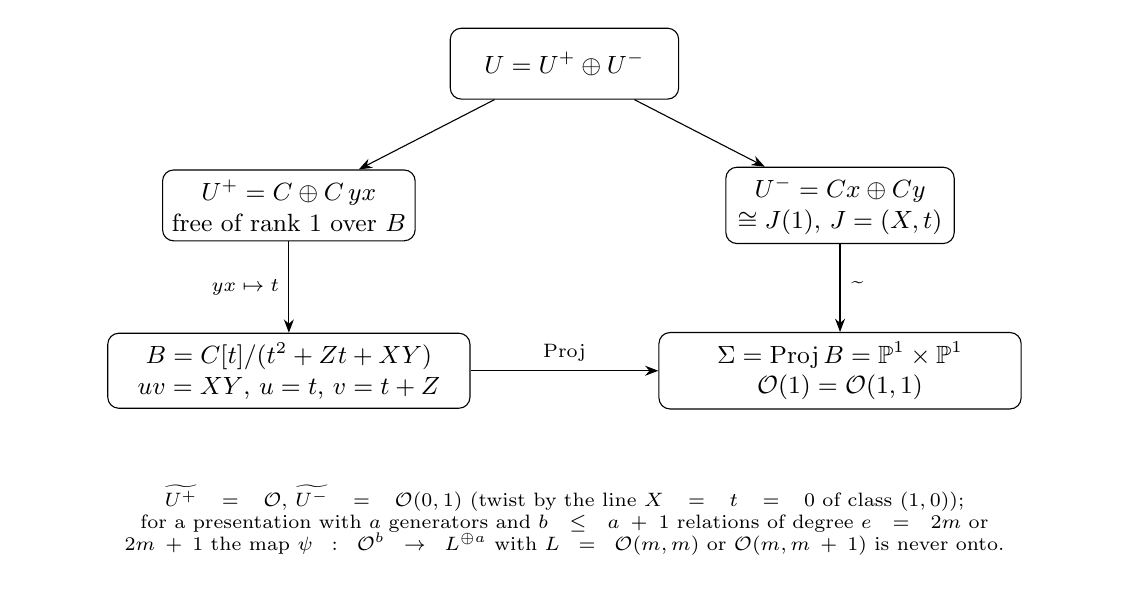
\begin{tikzpicture}[x=1cm,y=1cm,font=\small,>=Stealth]
\node[draw,rounded corners,minimum width=2.9cm,minimum height=0.9cm] (U) at (0,2.4) {$U=U^+\oplus U^-$};
\node[draw,rounded corners,minimum width=2.9cm,minimum height=0.9cm,align=center] (Up) at (-3.5,0.6) {$U^+=C\oplus C\,yx$\\ free of rank $1$ over $B$};
\node[draw,rounded corners,minimum width=2.9cm,minimum height=0.9cm,align=center] (Um) at (3.5,0.6) {$U^-=Cx\oplus Cy$\\ $\cong J(1)$, $J=(X,t)$};
\draw[->] (U) -- (Up); \draw[->] (U) -- (Um);
\node[draw,rounded corners,minimum width=4.6cm,minimum height=0.9cm,align=center] (B) at (-3.5,-1.5) {$B=C[t]/(t^2+Zt+XY)$\\ $uv=XY$, $u=t$, $v=t+Z$};
\node[draw,rounded corners,minimum width=4.6cm,minimum height=0.9cm,align=center] (S) at (3.5,-1.5) {$\Sigma=\operatorname{Proj}B=\mathbb{P}^1\times\mathbb{P}^1$\\ $\mathcal{O}(1)=\mathcal{O}(1,1)$};
\draw[->] (Up) -- node[left,font=\scriptsize]{$yx\mapsto t$} (B);
\draw[->] (Um) -- node[right,font=\scriptsize]{$\widetilde{\ \ }$} (S);
\draw[->] (B) -- node[above,font=\scriptsize]{$\operatorname{Proj}$} (S);
\node[font=\scriptsize,align=center,text width=13.4cm] at (0,-3.4) {$\widetilde{U^+}=\mathcal{O}$, $\widetilde{U^-}=\mathcal{O}(0,1)$ (twist by the line $X=t=0$ of class $(1,0)$);\\ for a presentation with $a$ generators and $b\le a+1$ relations of degree $e=2m$ or $2m+1$ the map $\psi:\mathcal{O}^b\to L^{\oplus a}$ with $L=\mathcal{O}(m,m)$ or $\mathcal{O}(m,m+1)$ is never onto.};
\end{tikzpicture}

\caption{The structure behind Theorem~C in characteristic $2$: the algebra $U$ splits as the even part $U^+$, free of rank one over $B=C[t]/(t^2+Zt+XY)$, and the odd part $U^-\cong J(1)$ with $J=(X,t)$; $\operatorname{Proj}B$ is the quadric surface $\mathbb P^1\times\mathbb P^1$, on which $U^+$ gives $\mathcal O$ and $U^-$ gives $\mathcal O(0,1)$; a presentation with $b\le a+1$ relations maps $\mathcal O^b$ to $L^{\oplus a}$ with $L$ ample, and the map is never onto.}
\label{fig:char2}
\end{figure}

\paragraph{Step 3: $M_{\mathcal P}$ is not of finite length.} Write $L=\mathcal N(m)$, that is $L=\mathcal O(m,m)$ for $e$ even and $L=\mathcal O(m,m+1)$ for $e$ odd, and let $\psi:\mathcal O^b\to L^{\oplus a}$ be the map of sheaves on $\Sigma$ given by $F_1,\dots,F_b$. Its cokernel is the sheaf of $M_{\mathcal P}$ twisted by $m$, $\widetilde{M_{\mathcal P}}(m)$. A finitely generated graded $B$-module of finite length is killed by a power of the irrelevant ideal, so its sheaf is $0$. Hence if $M_{\mathcal P}$ has finite length, $\psi$ is surjective at every point of $\Sigma$. Both bidegrees of $L$ are positive because $m\ge1$, so $L$ is ample and $L\cdot L=2m^2$ ($e$ even) or $2m(m+1)$ ($e$ odd) is positive.
\begin{itemize}
\item $b<a$: a surjection from a bundle of smaller rank does not exist.
\item $b=a$: $\psi$ is an isomorphism, since a surjection between locally free sheaves of equal rank is one, so its determinant gives $\mathcal O=L^{\otimes a}$, impossible for an ample $L$.
\item $b=a+1$: the kernel $K$ of $\psi$ is a line bundle and $0\to K\to\mathcal O^{a+1}\to L^{\oplus a}\to0$ is exact, so $c(K)\,c(L^{\oplus a})=1$ with $c(L^{\oplus a})=1+aL+\binom a2L\cdot L$. In degree $1$, $c_1(K)=-aL$; in degree $2$, $\binom a2L\cdot L+(aL)\cdot(-aL)=-\tfrac{a(a+1)}2L\cdot L=0$, which is impossible since $L\cdot L>0$.
\end{itemize}
Hence $\psi$ is not surjective at some point of the $k$-scheme $\Sigma$; the sheaf of $M_{\mathcal P}$ is not zero, its Krull dimension is at least $1$, and $M$ is not of finite length. Nothing uses the size of $k$. For $a=1$ and $b=2$ this is the statement that two curves of the same ample class on $\mathbb P^1\times\mathbb P^1$ meet. For $e$ even there is a proof without sheaves: $M_{\mathcal P}=\operatorname{coker}(B(-m)^b\to B^a)$ has support $V(I_a)$ with $I_a$ the ideal of $a\times a$ minors ($0$ if $b<a$); $I_a$ is generated by forms of degree $am>0$, so it is proper and of height at most $\max(0,b-a+1)\le2<3=\operatorname{ht}B_+$ by Eagon and Northcott, so $I_a$ is not primary to the irrelevant ideal and $M_{\mathcal P}$ has infinite length. The argument stops where it must: with $e=1$ ($m=0$, odd) $L=\mathcal O(0,1)$ has $L\cdot L=0$ and two sections of it need not meet (the trivial module), and with $b=a+2$ the expected codimension of the degeneracy locus is $3$ and the argument gives no obstruction.

\paragraph{Step 4: the corollaries.} The polynomial $1-2t^e+2t^{3e}-t^{4e}$ vanishes to order $3$ at $t=1$ and vanishes at $t=-1$, so a module with Betti table $(1,2,2,1)$ on $(0,e,3e,4e)$ has a polynomial Hilbert series and finite length; it is cyclic with two relations of degree $e$, that is $U/(Uf+Ug)$, which Theorem~\ref{thm:C} excludes with $a=1$, $b=2$. In general a module with a pure table on $(0,d_1,d_2,d_3)$ with $\beta_0=a$ and $\beta_1=b$ is $U^a$ modulo $b$ elements of degree $d_1$. Over $S$ the Fitting ideal argument of Lemma~\ref{lem:krull} gives $\beta_1\ge\beta_0+2$, which proves Corollary~\ref{cor:C2}; the list of the eight rays with $\beta_1=\beta_0+1$ is the enumeration of the degree sequences $0<d_1<d_2<d_3\le12$ with $\beta_1=\beta_0+1$, recomputed by the script [MV].

\subsubsection*{The eventual Hilbert function of a general presentation}

Let $\mathcal D$ be the locus where $\psi$ is not surjective. When $\mathcal D$ is finite and $\psi$ has corank at most $1$ at each of its points (automatic for $a=1$), the cokernel of $\psi$ is locally cyclic and its length is the degree of $\mathcal D$ with its determinantal structure: $L\cdot L$ for $a=1$, and by the Thom--Porteous formula for the corank-one locus of $\mathcal O^{a+1}\to L^{\oplus a}$ \cite{Fulton}, $c_1^2-c_2=\tfrac{a(a+1)}2L\cdot L$, the same number that obstructs surjectivity in step 3. Reducedness is not needed. So $\dim(M_{\mathcal P})_n=\frac{a(a+1)}2L\cdot L$ for large $n$ (Serre). The other parity has the same eventual dimension. The odd elements $x$, $y$ and $x+y$ have the central squares $X$, $Y$ and $X+Y+Z$, with no common zero on $\Proj C$. Each odd element $w$ satisfies $wt=(t+Z)w$ (by~\eqref{eq:mult}: $x\cdot yx=(yx+Z)x$ and $y\cdot yx=Yx=(yx+Z)y$), so $wb=\varsigma(b)w$ for the involution $\varsigma$ of $B$ that fixes $C$ and sends $t$ to $t+Z$, which exchanges the two rulings. Where $w^2$ does not vanish, left multiplication by $w$ is a $\varsigma$-semilinear isomorphism between the localizations of the two parities of any graded $U$-module, with inverse $w^{-2}w$. Hence the sheaves of the two parities have the same length and the Hilbert function of $M$ is eventually the number above in every degree. Table~\ref{tab:eventual} gives the predicted values.

\begin{table}[htbp]
\centering\footnotesize
\begin{tabular}{@{}lrrll@{}}
\toprule
presentation & $e$ & $m$ & predicted eventual value & number\\
\midrule
two quadrics & 2 & 1 & $2m^2=2$ & 2\\
two cubics & 3 & 1 & $2m(m+1)=4$ & 4\\
two quartics & 4 & 2 & $2m^2=8$ & 8\\
two quintics & 5 & 2 & $2m(m+1)=12$ & 12\\
$2\times3$ matrix of quadrics & 2 & 1 & $\tfrac{a(a+1)}{2}\cdot2=6$ & 6\\
$2\times3$ matrix of cubics & 3 & 1 & $\tfrac{a(a+1)}{2}\cdot4=12$ & 12\\
\bottomrule
\end{tabular}

\caption{Predicted eventual value of the Hilbert function in characteristic $2$ of a general presentation with $a$ generators and $a+1$ relations of degree $e=2m$ or $2m+1$: $\tfrac{a(a+1)}2L\cdot L$ with $L\cdot L=2m^2$ for even $e$ and $2m(m+1)$ for odd $e$; the values for two quadrics, two cubics and the $2\times3$ matrix of quadrics were derived before the experiment and are compared with it in Section~\ref{sec:results}.}
\label{tab:eventual}
\end{table}

\subsection{Lifting a prime-field realization to characteristic \texorpdfstring{$0$}{0}}
\label{sec:lift}

The census realizes many primitive points by a module over $\F_{32003}$. The following proposition gives an exact criterion under which such a module lifts to a module over $\Q$ with the same Betti table. Let $p$ be a prime, $S_R=R[u,v,w]$ for a ring $R$, and let $A$ be a homogeneous matrix with integer coefficients.

\begin{proposition}[Lift of a pure table]\label{prop:lift}
\emph{(a) Cokernel form.} For a field $k$ let $M_k=\operatorname{coker}\big(A\otimes k:S_k(-d_1)^b\to S_k^a\big)$. The piece $(M_k)_d$ is the cokernel of an integer matrix $A_d$ reduced to $k$, so $\dim(M_\Q)_d=\operatorname{rows}(A_d)-\operatorname{rank}_\Q(A_d)\le\operatorname{rows}(A_d)-\operatorname{rank}_p(A_d)=\dim(M_{\F_p})_d$. Suppose $M_{\F_p}$ has finite length and a pure Betti table $\beta$, and $\operatorname{rank}_\Q(A_d)=\operatorname{rank}_p(A_d)$ for every $d$ up to the top degree of $M_{\F_p}$. Then $M_\Q$ has finite length and the same Betti table.

\emph{(b) Image form.} Let $T_R=S_R/(u^{r+1},v^{r+1},w^{r+1})$, which is free over $R$, and let $N_k$ be the image of $A$ over $k$ between free $T_k$-modules. Then $\dim(N_k)_d$ is the rank over $k$ of an integer matrix $A_d$, so $\dim(N_\Q)_d\ge\dim(N_{\F_p})_d$. Suppose $N_{\F_p}$ has a pure Betti table $\beta$ as an $S$-module and $\operatorname{rank}_\Q(A_d)=\operatorname{rank}_p(A_d)$ for $0\le d\le r$ (outside this range both sides vanish). Then $N_\Q$ has the same Betti table.
\end{proposition}
\begin{proof}
Work over the local ring $\Z_{(p)}$. In (a) let $M=\operatorname{coker}(A\text{ over }\Z_{(p)})$; each $M_d$ is the cokernel of the integer matrix $A_d$, and equal ranks over $\Q$ and over $\F_p$ mean that $M_d$ has no $p$-torsion, so it is free of finite rank over $\Z_{(p)}$. In (b) let $N$ be the image of $A$ over $\Z_{(p)}$, torsion free in each degree; equal ranks mean that the cokernel of $A_d$ has no $p$-torsion, so $N_d\otimes\F_p$ injects into the target and equals the image of $A_d$ over $\F_p$. In both cases there is a graded $S_{(p)}$-module $X$, free of finite rank over $\Z_{(p)}$ in each degree, with $X\otimes\F_p$ the module over $\F_p$ and $X\otimes\Q$ the module over $\Q$. Take a minimal graded free resolution of $X\otimes\F_p$. Lift its generators to $X$ (Nakayama over $\Z_{(p)}$, degree by degree); the kernel $K$ of the resulting surjection $F_0\to X$ is again free over $\Z_{(p)}$ in each degree, and $K\otimes\F_p$ is the kernel over $\F_p$ because $\Tor_1^{\Z_{(p)}}(X_d,\F_p)$ vanishes. Repeating gives a graded free resolution of $X$ over $S_{(p)}$ whose reduction is the minimal resolution over $\F_p$. The minimal resolution over $\F_p$ has length $3$, so after three steps the next kernel reduces to zero modulo $p$; being free of finite rank over $\Z_{(p)}$ in each degree, it is zero, and the lifted resolution has length $3$. Tensoring with $\Q$ (flat) gives a free resolution of the module over $\Q$ with the same graded ranks, so $\beta_{ij}(\Q)\le\beta_{ij}(\F_p)$ for all $i,j$. The Hilbert functions are equal, so for each $j$ the alternating sums over $i$ agree; the table over $\F_p$ is pure, so for each $j$ at most one $i$ has $\beta_{ij}(\F_p)$ nonzero, and the inequality forces equality. In (a) $M_\Q$ vanishes in every degree where $M_{\F_p}$ does (it is generated in degree $0$ and its pieces are no larger), so it has finite length; in (b) $N_\Q$ is a submodule of a module of finite length.
\end{proof}

The converse is not claimed: unequal ranks say that this lift is not flat at $p$, and not that the ray fails over $\Q$. The proposition is derived on paper [D], re-derived independently, and consistent with the $64$ hits whose rational recheck completed and the two modules resolved over $\Q$ in Singular. The condition it requires is an exact computation [MV] (Section~\ref{sec:rank}): the rank over $\F_{32003}$ is maximal in every degree the proposition needs, which forces the rank over $\Q$. By base change from $\Q$, a pure table over $\Q$ is the table over every field of characteristic $0$. The statement on the rays with $d_3\le9$ (Proposition~\ref{prop:lownine}) does not use this proposition: every module on which it rests has a resolution over $\Q$ computed in two systems.

\subsection{The locus of pure pairs of forms}
\label{sec:family}

The modules $M_e$ of Theorem~\ref{thm:A} are one pure module for each pair of points of the projective line, and the question is whether they are all. The notation is that of Section~\ref{sec:pairsetting}: $G_e=\operatorname{Gr}(2,U_e)$, $\mu_n(W)$, $h_e(n)$, $r=2u(2e)-2$, $D_e$ of~\eqref{eq:De}, $P_e$ the set of pure spaces and $W_0=\langle x^e,y^e\rangle$.

\begin{thmletter}\label{thm:family}
Let $e\ge2$, let $k$ be algebraically closed, and let $D_e\subset G_e$ be the locus of~\eqref{eq:De}.
\begin{enumerate}
\item[(a)] Every irreducible component of $D_e$ has codimension at most $2h_e(3e)$ in $G_e$.
\item[(b)] $P_e\subset D_e$, and $P_e$ is open in $D_e$, in every characteristic.
\item[(c)] Hence every irreducible component of $P_e$ has dimension at least $4e-4$: $4$ and $8$ for $e=2,3$ (where $P_e$ is open in $G_e$) and $12,16,20,24$ for $e=4,5,6,7$. The bound concerns the components of $D_e$ that meet $P_e$.
\item[(d)] If $\ch k=0$ or $\ch k\ge2e$, then $W_0\in P_e$ (Theorem~\ref{thm:A}), $P_e$ is stable under the graded automorphisms of $U$, and the orbit of $W_0$ has dimension $2$. So for $e\ge4$ the pure cyclic modules on the ray $(0,e,3e,4e)$ form a family of dimension at least $4e-4$ in which the modules $U/U(l_1^e,l_2^e)$ form a subfamily of dimension $2$: up to automorphism there are at least $4e-7$ parameters of pure modules ($9$ at $e=4$).
\end{enumerate}
\end{thmletter}

\begin{proof}
\emph{(a).} On $G_e$ let $\mathcal S$ be the tautological subbundle of rank $2$. Left multiplication is a map of vector bundles $\mu_{3e}:U_{2e}\otimes\mathcal S\to U_{3e}\otimes\mathcal O$, of ranks $m=2u(2e)$ and $n=u(3e)$. The locus $D_e$ is its locus of rank at most $r$, and $r\le\min(m,n)$ because $h_e(3e)\ge0$. Locally on $G_e$ the bundle map is a morphism $\varphi$ from an open set of $G_e$ to the space of $m\times n$ matrices, and $D_e$ is the preimage of the variety $Y_r$ of matrices of rank at most $r$, which is irreducible of codimension $(m-r)(n-r)$: it is the closure of the set of matrices of rank exactly $r$, a single orbit of $\mathrm{GL}_m\times\mathrm{GL}_n$ and so irreducible, of dimension $r(m-r)+rn=r(m+n-r)$ (a column space, then a map onto it), and $mn-r(m+n-r)=(m-r)(n-r)$ (see also~\cite{BV} for determinantal varieties). The preimage is the intersection of the graph of $\varphi$ with $G_e\times Y_r$ inside the smooth variety $G_e\times\{m\times n\text{ matrices}\}$, so each of its components has dimension at least $\dim G_e-(m-r)(n-r)$ (the dimension of an intersection in a smooth variety). Here $(m-r)(n-r)=2\,(u(3e)-2u(2e)+2)=2h_e(3e)$.

\emph{(b), the inclusion.} Let $W$ be pure. Its minimal resolution has two second syzygies, in degree $3e$, and none below, so $\mu_n(W)$ is injective for $n<3e$ and the kernel of $\mu_{3e}(W)$ has dimension $2$: $\operatorname{rank}\mu_{3e}(W)=r$ and $W\in D_e$.

\emph{(b), openness.} Let $W_1$ be pure. The following conditions define a subset $V$ of $D_e$ that contains $W_1$, and each is open in $D_e$:
\begin{enumerate}
\item $\mu_n(W)$ is injective for $e\le n<3e$ (maximal rank);
\item $\operatorname{rank}\mu_{3e}(W)\ge r$ (so the rank is $r$ on $V$, and $K(W)=\ker\mu_{3e}(W)$ is a vector bundle of rank $2$ on $V$ with its reduced structure);
\item for $3e<n\le4e+1$, $\operatorname{rank}\mu_n(W)\ge u(n)-h_e(n)$;
\item for $3e<n\le4e+1$, the map $\nu_n(W):U_{n-3e}\otimes K(W)\to U_{n-e}\otimes W$ (left multiplication of the two syzygies) has rank at least $2u(n-3e)-u(n-4e)$, its rank at $W_1$.
\end{enumerate}
Conditions~1, 2 and~3 are lower bounds on the rank of a map of vector bundles, and so is~4 on the locus of~2. At $W_1$ they hold with equality, by the pure resolution: the kernel of $\mu_n(W_1)$ is the image of $\nu_n(W_1)$, and the kernel of $\nu_n(W_1)$ is the third syzygy, of dimension $u(n-4e)$ ($U$ is a domain). On $V$ the image of $\nu_n(W)$ lies in the kernel of $\mu_n(W)$, because $\mu$ is linear for left multiplication, so $\operatorname{rank}\mu_n(W)\le2u(n-e)-(2u(n-3e)-u(n-4e))=u(n)-h_e(n)$ for $3e<n\le4e+1$; with~3 this is an equality. So $H_W(n)=h_e(n)$ for every $n\le4e+1$. Since $h_e(n)=0$ for $n\ge4e-3$ and $M_W$ is generated in degree $0$, $M_W$ vanishes from degree $4e-3$ on, and $H_W=h_e$.

So $V$ is a neighbourhood of $W_1$ in $D_e$ on which the Hilbert function is constant. Over $V$ with its reduced structure the graded pieces of $M_W$ are vector bundles, and the graded Betti numbers $\beta_{i,j}(W)=\dim\Tor_i^U(k,M_W)_j$, computed from the finite free resolution of the trivial module tensored with $M_W$, are upper semicontinuous on $V$. Only the finitely many $(i,j)$ with $i\le3$ and $j\le4e$ can be nonzero on $V$, since $M_W$ vanishes from degree $4e-3$ on. For $W\in V$ the Betti numbers are at least those of the pure table: $M_W$ has one generator, in degree $0$, and two minimal relations, in degree $e$ (automatic for $W$ of dimension $2$); the trivial module has a resolution of length $3$; and the Hilbert series fixes the alternating sums, so $\beta_{2,j}-\beta_{3,j}$ is $2$ for $j=3e$, $-1$ for $j=4e$ and $0$ otherwise, which gives $\beta_{2,3e}\ge2$ and $\beta_{3,4e}\ge1$. At $W_1$ the Betti numbers are those of the pure table, so by semicontinuity they are on a neighbourhood of $W_1$ in $V$. That neighbourhood lies in $P_e$.

\emph{(c)} follows from (a) and (b): the components of $P_e$ are its nonempty intersections with the components of $D_e$, each open in its component, and $\dim G_e-2h_e(3e)=2u(e)-4-2h_e(3e)=4e-4$ by~\eqref{eq:fourE}.

\emph{(d).} The graded automorphisms of $U$ are $\mathrm{GL}_2$ acting on $U_1$ (the relations $[x,[x,y]]=[y,[x,y]]=0$ span a stable space), with $z\mapsto\det(g)z$; the scalars act on $U_e$ by a scalar, hence trivially on $G_e$. A twist by a graded automorphism preserves Betti tables, so $P_e$ is stable and the orbit of $W_0$ lies in $P_e$. The stabilizer of $W_0$ in $\mathrm{PGL}_2$ contains the diagonal torus, and $W_0$ determines the pair of points $\{x=0\},\{y=0\}$ of the projective line: the coefficient of the PBW monomial $x^{e-1}y$ in $(ax+by)^e$ (equivalently, in its image in $U/(z)=k[x,y]$) is $e\,a^{e-1}b$, and that of $xy^{e-1}$ is $e\,ab^{e-1}$, so $l^e$ lies in $W_0$ only for $l$ a multiple of $x$ or of $y$, in characteristic $0$ or larger than $e$. So the stabilizer has dimension $1$ and the orbit, the set of unordered pairs of distinct points, has dimension $2$. (In characteristic $p=e$ every line has its $e$-th power in $W_0$; the hypothesis of (d) excludes that case.)
\end{proof}

\begin{remark}[{The common-factor locus}]\label{rem:common}
For $e\ge4$ the locus $D_e$ is not of the expected codimension $2h_e(3e)$. If the images of a basis of $W$ in $U/(z)=k[x,y]$ share a factor $q$ of degree $\delta$, then $M_W$ maps onto $k[x,y]/(q)$, of dimension $\delta$ in every degree from $\delta-1$ on, so $\operatorname{rank}\mu_{3e}(W)\le u(3e)-\delta$. With $\delta=h_e(3e)$ this puts the common-factor locus $R_e$ inside $D_e$; $R_e$ has codimension $h_e(3e)$ in $G_e$, less than $2h_e(3e)$, and its modules have infinite length, so it contains no pure point. At $e=4$ it is the resultant hypersurface. Hence $D_e$ is not of the expected codimension for $e\ge4$ and is not empty in any characteristic. It is reducible at $e=4$ whenever it has a pure point (then $D_4\ne G_4$ is a closed set of dimension at most $13$ that contains the irreducible hypersurface $R_4$ and a point outside it), and for $e=4,\dots,7$ over $\Q$, where the component through $W_0$ has dimension $4e-4<\dim R_e$ (Proposition~\ref{prop:exact}); for $e\ge8$ its reducibility is not shown. A random $W$ over $\F_q$ lies in $D_4$ with probability of the order of $1/q$ and not $q^{-2}$ (Section~\ref{sec:resodd}); the Thom--Porteous formula for the expected codimension therefore does not compute a class of $D_e$. Statements (a) to (d) are not affected, since $W_0\notin R_e$: $x^e$ and $y^e$ are coprime. [D] for the inclusion; [MV] for the rank and the infinite length of $20$ random spaces of $R_e$ at $e=4$, and for the rank of $20$ at $e=5$ and $20$ at $e=6$ (Table~\ref{tab:sevenfam}).
\end{remark}

\begin{remark}[{What Theorem D does not say}]
For $e=2,3$ one has $h_e(3e)=0$ and $D_e=G_e$: the pure Hilbert function is the maximal-rank function and $P_e$ is open in $G_e$ (it is empty in characteristic $2$ by Theorem~\ref{thm:C}). The theorem says nothing about odd characteristic below $2e$: there $P_e$ is open in $D_e$ as well, but no pure point is known in advance; Proposition~\ref{prop:odd} exhibits some. It does not say that $P_e$ or $D_e$ is irreducible, what the exact dimension of $P_e$ is, or that $P_e$ is smooth; Proposition~\ref{prop:exact} answers the last two questions at the single point $W_0$ for $e=4,\dots,7$ over $\Q$. A count over a finite field tests (c) heuristically: if a component of $P_4$ of dimension $12$ is defined over $\F_q$ and geometrically irreducible, a random $W$ over $\F_q$ is pure with probability of the order of $q^{-2}$, since $\dim G_4=14$; the comparison with the measured shares is reported in Section~\ref{sec:resodd} as a heuristic and not as a test of a theorem.
\end{remark}

\begin{proposition}[Exact dimension at $W_0$]\label{prop:exact}
Let $e\in\{4,5,6,7\}$ and $k=\Q$. The Zariski tangent space of the determinantal scheme $D_e$ at $W_0$ has dimension exactly $4e-4$ ($12,16,20,24$). Consequently $D_e$ is smooth of dimension $4e-4$ at $W_0$, exactly one irreducible component of $D_e$ and of $P_e$ passes through $W_0$, and its dimension is $4e-4$.
\end{proposition}
\begin{proof}
The tangent dimension is the output of Algorithm~\ref{alg:tangent} (Table~\ref{tab:seventangent}): $\operatorname{rank}A=r$, $\dim K=2$, $\dim\operatorname{coker}A=h_e(3e)$, and $\operatorname{rank}T=2h_e(3e)$, so $T$ is onto and equality holds in~\eqref{eq:tangentdim} [MV]. By Theorem~\ref{thm:family}(a) and~(b) every component of $D_e$ through $W_0$ has dimension at least $4e-4$, and the dimension of the Zariski tangent space at a point is at least the dimension of every component through it. Equality of the two numbers makes the local ring of $D_e$ at $W_0$ regular of dimension $4e-4$; a regular local ring is a domain, so one component passes through $W_0$, and $P_e$ is open in $D_e$ and contains $W_0$ (Theorem~\ref{thm:A}). The tangent dimension of a point defined over $\Q$ does not change under the extension to $\overline\Q$. [D, from the machine value]
\end{proof}

The exactness depends on the characteristic: over $\F_{13}$ at $e=6$ and over $\F_{17}$ at $e=7$, both characteristics at least $2e$, the tangent space is larger by $2$ ($22$ and $26$, Table~\ref{tab:seventangent}). Nothing is concluded for those fields, where the locus need not be smooth at $W_0$.

The point $W_0$ has a four-parameter family of deformations that stay in $D_e$ and are pure in general, which makes the family of Theorem~\ref{thm:family} explicit for every $e\ge4$. For $a,b,c,d\in k$ put
\begin{equation}\label{eq:Le}
L_e(a,b,c,d)=\big\langle x^e+a\,xy^{e-1}+b\,y^{e-2}z,\ \ y^e+c\,x^{e-1}y+d\,x^{e-2}z\big\rangle\subset U_e .
\end{equation}

\begin{proposition}[A linear family of pure pairs]\label{prop:linear}
Let $e\ge4$ and let $k$ be a field of characteristic $0$ or at least $2e$.
\begin{enumerate}
\item[(i)] $L_e(a,b,c,d)\in D_e$ for every $(a,b,c,d)\in k^4$. (The proof is over an infinite field; a rank does not change under an extension of the field, so the statement holds over every field of these characteristics.)
\item[(ii)] If $k$ is algebraically closed, $L_e(a,b,c,d)$ is pure for $(a,b,c,d)$ in a nonempty Zariski open subset of $k^4$ that contains the origin.
\item[(iii)] $L_e(a,b,c,d)$ lies in the orbit of $W_0$ under the graded automorphisms only for $(a,b,c,d)=0$ (this part needs only characteristic $0$ or larger than $e$).
\end{enumerate}
So for every $e\ge4$ the modules $U/U\,L_e(a,b,c,d)$ with general parameters are pure of type $(0,e,3e,4e)$ with Betti table $(1,2,2,1)$ and are not of the form $U/U(l_1^e,l_2^e)$.
\end{proposition}

\begin{proof}
The monomials $x^ay^bz^c$ are written in the product order.

\emph{Step 1: the torus and the chart.} The torus $\Theta$ of pairs $t=(t_1,t_2)$ acts on $U$ by the graded automorphisms $x\mapsto t_1x$, $y\mapsto t_2y$, $z\mapsto t_1t_2z$; the monomial $m=x^ay^bz^c$ is an eigenvector with character $\chi_m=t_1^{a+c}t_2^{b+c}$. $\Theta$ fixes $W_0$. In the chart $W=\langle x^e+f,\ y^e+g\rangle$ around $W_0$ ($f,g$ in the span of the monomials of degree $e$ other than $x^e$ and $y^e$, with coordinates $f_m,g_m$), $t\,W=\langle x^e+t_1^{-e}t(f),\ y^e+t_2^{-e}t(g)\rangle$. Since $a+b+2c=e$, the coordinate $f_m$ is multiplied by $t_1^{a+c-e}t_2^{b+c}=s^{\,b+c}$ and $g_m$ by $t_1^{a+c}t_2^{b+c-e}=s^{-(a+c)}$, where $s=t_2/t_1$; call these exponents the weights of the coordinates. Every chart coordinate has a weight of absolute value between $1$ and $e-1$, and the weights $e-1$ and $-(e-1)$ occur exactly at the four coordinates of $L_e$: $f$ at $xy^{e-1}$ and at $y^{e-2}z$ (weight $e-1$), and $g$ at $x^{e-1}y$ and at $x^{e-2}z$ (weight $-(e-1)$).

\emph{Step 2: the characters of the resolution.} Grade $U$ by pairs of integers, $x$ in degree $(1,0)$, $y$ in $(0,1)$, $z$ in $(1,1)$ (the relation $yx=xy-z$ is homogeneous); $x^e,y^e$ are homogeneous, so $M_e$ is bigraded. A minimal bigraded free resolution of $M_e$ exists ($U$ is connected graded) and is a minimal graded resolution for the total degree, so by Theorem~\ref{thm:A} its generators have total degrees $0$; $e,e$; $3e,3e$; $4e$. Write their characters as $1$; $t_1^e,t_2^e$; $\sigma_1,\sigma_2$; $\sigma_3$ with $\sigma_j=t_1^{p_j}t_2^{q_j}$, $p_j+q_j=3e$ for $j=1,2$ and $p_3+q_3=4e$. With the character $1/((1-t_1)(1-t_2)(1-t_1t_2))$ of $U$, the character of $M_e$ is $\Delta/((1-t_1)(1-t_2)(1-t_1t_2))$ with $\Delta=1-t_1^e-t_2^e+\sigma_1+\sigma_2-\sigma_3$. $M_e$ has finite length, so its character is a polynomial and $\Delta$ vanishes at $t_1=1$ and at $t_2=1$. At $t_1=1$: $t_2^{q_1}+t_2^{q_2}=t_2^e+t_2^{q_3}$, so $\{q_1,q_2\}=\{e,q_3\}$. At $t_2=1$: $\{p_1,p_2\}=\{e,p_3\}$. Label so that $q_1=e$; then $p_1=2e\ne e$, so $p_1=p_3$ and $p_2=e$, hence $q_2=2e=q_3$. So $\sigma_1=t_1^{2e}t_2^e$, $\sigma_2=t_1^et_2^{2e}$, $\sigma_3=(t_1t_2)^{2e}$, and $\Delta=(1-t_1^e)(1-t_2^e)(1-(t_1t_2)^e)$: the character of $M_e$ is the sum of $t_1^{a+c}t_2^{b+c}$ over $0\le a,b,c\le e-1$.

In degree $3e$: the kernel $K$ of $A=\mu_{3e}(W_0)$ (the pairs $(u_1,u_2)\in U_{2e}^2$ with $u_1x^e+u_2y^e=0$) is the space of second syzygies in degree $3e$, with characters $t_1^{2e}t_2^e$ and $t_1^et_2^{2e}$. The cokernel $Q=(M_e)_{3e}$ has the characters $t_1^{\alpha}t_2^{3e-\alpha}$ with $\alpha=a+c$ over the triples with $a+b+2c=3e$ and $0\le a,b,c\le e-1$. From $b=3e-\alpha-c\le e-1$ and $c\le e-1$ follows $\alpha\ge e+2$; from $a=\alpha-c\le e-1$ and $c\le e-1$ follows $\alpha\le2e-2$. So every $\alpha$ lies between $e+2$ and $2e-2$.

\emph{Step 3: the local equations are semi-invariants of small weight.} Identify $W$ with $W_0$ through the basis of the chart, so that $\mu(W)=\mu_{3e}(W)$ is a map from $E=U_{2e}\otimes W_0$ to $U_{3e}$, $u\otimes x^e\mapsto u(x^e+f)$ and $u\otimes y^e\mapsto u(y^e+g)$. With $\rho_E(t)$ the action of $t$ on $E$ and $\rho(t)$ on $U_{3e}$, $\mu(tW)=\rho(t)\mu(W)\rho_E(t)^{-1}$: for the first generator $u(x^e+t_1^{-e}t(f))=t_1^{-e}t\big(t^{-1}(u)(x^e+f)\big)$, and likewise for the second. $\Theta$ acts diagonally on $E$ and on $U_{3e}$, so $E=K\oplus K'$ and $U_{3e}=Q'\oplus I$ with all four subspaces $\Theta$-stable, $I=\operatorname{im}A$, and $Q'$ a complement of $I$ mapped isomorphically to $Q$. In these decompositions $\mu(W)$ has the blocks $A_{11}(W):K\to Q'$, $A_{12}(W):K'\to Q'$, $A_{21}(W):K\to I$, $A_{22}(W):K'\to I$, with $A_{22}(W_0)$ bijective ($\dim K'=r=\dim I$) and the other three zero at $W_0$. The set where $A_{22}$ is invertible is open and $\Theta$-stable ($\det A_{22}(tW)$ is $\det A_{22}(W)$ times a character of $\Theta$), and on it $\operatorname{rank}\mu(W)\le r$ if and only if the Schur complement $\Xi(W)=A_{11}-A_{12}A_{22}^{-1}A_{21}:K\to Q'$ vanishes. The equivariance of $\mu$ gives $\Xi(tW)=\rho(t)\,\Xi(W)\,\rho_E(t)^{-1}$: the entry $F$ of $\Xi$ from the eigenvector of $K$ with character $t_1^pt_2^q$ to the eigenvector of $Q'$ with character $t_1^{\alpha}t_2^{3e-\alpha}$ satisfies $F(tW)=t_1^{\alpha-p}t_2^{3e-\alpha-q}F(W)$ on that set. For $(p,q)=(2e,e)$ the factor is $s^{2e-\alpha}$, for $(p,q)=(e,2e)$ it is $s^{e-\alpha}$. By step 2 these weights lie between $2$ and $e-2$, or between $-(e-2)$ and $-2$.

\emph{Step 4: vanishing on the family.} Let $k$ be infinite. $\det A_{22}$ is a polynomial in the chart coordinates that is multiplied by a character under $\Theta$ and is not zero at the fixed point $W_0$, so that character is trivial; each entry $F$ is $P/(\det A_{22})^{m}$ with $P$ a polynomial in the coordinates multiplied by $s^{w}$ under $\Theta$, $w$ the weight of $F$. Comparing coefficients ($k$ is infinite), every monomial of $P$ in the coordinates has total weight $w$. On the coordinate subspace $L_e$ every monomial has a weight that is a multiple of $e-1$ (step 1). The weights $w$ are nonzero and of absolute value at most $e-2$, so none is a multiple of $e-1$: the restriction of each $P$ to $L_e$ is zero. So $\Xi$ vanishes on the nonempty open subset of $L_e$ where $A_{22}$ is invertible, which therefore lies in $D_e$; $D_e$ is closed and $L_e$ (an affine space) is irreducible, so $L_e$ lies in $D_e$. This is (i).

\emph{Step 5: general members are pure.} $P_e$ is open in $D_e$ in every characteristic (Theorem~\ref{thm:family}(b)) and contains $W_0$, the member with parameters $0$, which is pure by Theorem~\ref{thm:A}. So the pure members of $L_e$ form an open subset of $k^4$ that contains the origin. This is (ii).

\emph{Step 6: the orbit.} The graded automorphisms of $U$ are $\mathrm{GL}_2$ acting on $U_1=\langle x,y\rangle$, so the orbit of $W_0$ is the set of $\langle l_1^e,l_2^e\rangle$ with $l_1,l_2$ independent linear forms in $x,y$. Let $W=L_e(a,b,c,d)$ be one of them. The image of $W$ in $U/(z)=k[x,y]$ is spanned by $x^e+a\,xy^{e-1}$ and $y^e+c\,x^{e-1}y$, whose coefficients at $x^{e-2}y^2$ vanish ($2\le e-2$ since $e\ge4$). The image of $(\alpha x+\beta y)^e$ has the coefficient $\binom e2\alpha^{e-2}\beta^2$ there, and $\binom e2$ is not zero in characteristic $0$ or larger than $e$. So each $l_j$ is a multiple of $x$ or of $y$, $W=\langle x^e,y^e\rangle$, and $(a,b,c,d)=0$. This is (iii). A graded isomorphism between cyclic modules generated in degree $0$ sends the generator to a multiple of the generator, so the modules $U/UW$ are of the form $U/U(l_1^e,l_2^e)$ only for $W$ in the orbit.
\end{proof}

\begin{remark}[{Limits of Proposition~\ref{prop:linear}}]
The argument uses Theorem~\ref{thm:A} twice, for the total degrees of the resolution (step 2) and for the purity of $W_0$ (step 5). It says nothing in characteristic below $2e$, and it does not extend there as it stands: steps~2 and~3 use the resolution of Theorem~\ref{thm:A}, and in every case computed ($e=4,\dots,7$, odd $p<2e$) $\operatorname{rank}\mu_{3e}(W_0)<r$, so the kernel of $\mu_{3e}(W_0)$ is larger than the two syzygies of step~2. For $e=4$ the weights of step 3 are $2$ and $-2$ ($\alpha=6$), and for $e=5$ they are $2,3,-2,-3$ ($\alpha=7,8$). $L_e$ is the largest coordinate subspace of the chart to which the argument applies: it consists of the coordinates of extreme weight $\pm(e-1)$, and every other coordinate has a weight whose multiples meet the weights of the equations. The torus identifies $L_e(a,b,c,d)$ with $L_e(s^{e-1}a,s^{e-1}b,s^{-(e-1)}c,s^{-(e-1)}d)$, so up to that action the family has three parameters; whether other automorphisms identify more members is not examined. Not claimed: which members are pure (the open set is not described, and members of rank below $r$ exist, Table~\ref{tab:sevenfam}), anything about the other components of $D_e$, or smoothness. The proposition is proved for every $e\ge4$ [D] and checked by machine for $e=4$ and $e=5$ (Section~\ref{sec:resfamily}) [MV].
\end{remark}

\subsection{Odd characteristic below \texorpdfstring{$2e$}{2e}: explicit pure pairs}
\label{sec:oddchar}

In odd characteristic $p<2e$ the module $M_e$ is not pure (Theorem~\ref{thm:A}), and Theorem~\ref{thm:family} gives no pure point there. The following statement is an existence result by exhibiting pairs.

\begin{proposition}\label{prop:odd}
Let $(e,p)\in\{(3,3),(3,5),(4,3),(4,5),(4,7),(5,3),(5,5),(5,7),(6,3)\}$ and let $f,g\in U_e$ be the forms of the corresponding row of Table~\ref{tab:sixpairs}, with coefficients in $\F_p$. Then $U/(Uf+Ug)$ has length $e^3$ and the pure Betti table $(1,2,2,1)$ on $(0,e,3e,4e)$, over $\F_p$ and over every field of characteristic $p$.
\end{proposition}
\begin{proof}
The module is cyclic with two relations of degree $e$. Its Hilbert function is recomputed by exact elimination in this paper's script from the stored basis, whose terms are the printed forms, in the basis of Section~\ref{sec:exactU}, and equals $h_e(n)$ for $0\le n\le4e-3$ with $h_e(4e-3)=0$ [MV]; so its length is $e^3$. The Betti table is computed by the Tor complex of Section~\ref{sec:tor} in the exact library and by Singular, and both give $(1,2,2,1)$ on $(0,e,3e,4e)$ [MV]. Betti numbers do not change under extension of the base field, since $\Tor$ commutes with flat base change.
\end{proof}

\begin{corollary}\label{cor:ray}
For $e\in\{2,3,4,5\}$ the point $(1,2,2,1)$ of the ray $(0,e,3e,4e)$ is the Betti table of a finite length module over $U\otimes k$ if and only if $\ch k\ne2$.
\end{corollary}
\begin{proof}
If $\ch k=2$ no such module exists by Corollary~\ref{cor:C1}. If $\ch k=0$ or $\ch k\ge2e$ the module $M_e$ realizes the point (Theorem~\ref{thm:A}). The remaining odd characteristics are $p=3$ for $e=2$, $p=3,5$ for $e=3$, $p=3,5,7$ for $e=4$ and $p=3,5,7$ for $e=5$. For $e=2$, $p=3$ pairs of quadrics with the table exist (Remark~\ref{rem:charthree}) [MV]; for the others Proposition~\ref{prop:odd} gives the pair.
\end{proof}

At $e=6$ the pair over $\F_3$ of Table~\ref{tab:sixpairs} realizes the point $(1,2,2,1)$ of $(0,6,18,24)$ in characteristic $3$, and Theorems~\ref{thm:A} and~\ref{thm:C} cover characteristic $0$ and at least $12$ and characteristic $2$; the characteristics $5$ and $11$ are settled by Corollary~\ref{cor:cases} and by the linear family (Section~\ref{sec:reslf}), and the characteristic $7$ by the search in the strata (Section~\ref{sec:resstrata}). At $e=7$ the characteristics $3,7,11,13$ are settled by Corollary~\ref{cor:cases} and the linear family, and $5$ by the search in the strata (Section~\ref{sec:state}). The search of Section~\ref{sec:resodd} in the whole space does not reach $e=6$ over $\F_5$: by the heuristic comparison the share of pure spaces there is of the order of $5^{-8}\approx2.6\times10^{-6}$, so that the early stop at $40$ pure spaces would take of the order of $10^{7}$ random spaces [C]; the weight-class strata reduce the space searched, and that is how the pairs of Section~\ref{sec:resstrata} were found. A statement for every $e$ and every odd $p<2e$ needs a construction, and none is known: Corollary~\ref{cor:cases} reaches the primes dividing $e(e-1)$ and Corollary~\ref{cor:scale1} the multiples of settled degrees. The dimension bound of Theorem~\ref{thm:family} makes it plausible that a search over a small field finds such pairs [C]; a locus that is nonempty over the algebraic closure need not have points over a given prime field.

\subsection{Pure pairs that are homogeneous for the class weight: a necessary condition}
\label{sec:strata}

The grading of Section~\ref{sec:rings} by the class weight gives a necessary condition for purity that does not see the characteristic, and it says where a pure pair with a cyclic symmetry can lie. Notation: $u(n)$, $G_e$, $\mu_n(W)$, $W_0$, $h_e$ and $r$ are those of Section~\ref{sec:pairsetting}; $u_k(n)$ is the dimension of the part of $U$ of degree $n$ and class $k$ modulo $m$ (Section~\ref{sec:rings}). For $m\ge2$ and classes $i,j$ modulo $m$ the \emph{stratum} is
\begin{equation}\label{eq:stratum}
S(m;i,j)=\{\langle f,g\rangle\in G_e:\ f\in U_{(e,[i])},\ g\in U_{(e,[j])}\}.
\end{equation}
Over a field that contains the $m$-th roots of unity and whose characteristic does not divide $m$ the union of the strata $S(m;i,j)$ is the fixed locus on $G_e$ of the points of the subgroup $\mu_m$ of the torus; for the group scheme $\mu_m$ no assumption is needed, since a grading by classes modulo $m$ is an action of $\mu_m$. The definition by supports needs neither assumption and is the one used. Three examples. The power pair $W_0$ lies in $S(m;0,e\bmod m)$ for every $m$, since $x^e$ has weight $0$ and $y^e$ has weight $e$. The linear family $L_e$ of~\eqref{eq:Le} is the affine chart ``the coefficients of $x^e$ and of $y^e$ equal $1$'' of $S(e-1;0,1)$: the monomials of degree $e$ and weight $0$ or $e-1$ are $x^e$, $xy^{e-1}$ and $y^{e-2}z$, and those of weight $1$ or $e$ are $x^{e-1}y$, $x^{e-2}z$ and $y^e$. And $S(e+1;0,e)$ is the single point $W_0$. The automorphism that exchanges $x$ and $y$ and sends $z$ to $-z$ sends the weight $w$ to $e-w$ on $U_e$, so it sends $S(m;i,j)$ to $S(m;e-i,e-j)$.

\begin{proposition}[Homogeneous resolution]\label{prop:strata}
Let $W=\langle f,g\rangle$ be a pure pair of forms of degree $e$ (the module $M=U/(Uf+Ug)$ has the Betti table $(1,2,2,1)$ on $(0,e,3e,4e)$) with $f\in U_{(e,[i])}$ and $g\in U_{(e,[j])}$ for some $m\ge2$. Then there are classes $s_1,s_2,t$ modulo $m$ such that for every degree $n$ and every class $k$
\begin{equation}\label{eq:Hk}
H_k(n):=u_k(n)-u_{k-i}(n-e)-u_{k-j}(n-e)+u_{k-s_1}(n-3e)+u_{k-s_2}(n-3e)-u_{k-t}(n-4e)\ \ge\ 0,
\end{equation}
and $H_k(n)$ is the dimension of the part of $M$ of degree $n$ and class $k$. In particular $\sum_kH_k(n)=h_e(n)$. [D]
\end{proposition}
\begin{proof}
The left ideal $I=Uf+Ug$ is generated by elements that are homogeneous for the grading by (degree, class), so $I$ and $M=U/I$ are graded for it. $M$ has a minimal free resolution by free modules with homogeneous generators and homogeneous maps for this finer grading: at each step one chooses a minimal system of generators of the kernel that is homogeneous for the finer grading, which is possible because the kernel of a homogeneous map is graded and, in each degree $n$, a complement of the part generated in lower degrees can be chosen as a sum of its class components. A resolution built this way is minimal for the grading by degree alone (its maps have no entry of degree $0$), and the minimal resolution for the degree is unique up to isomorphism, so its ranks in each degree are the Betti numbers of $M$: one generator in degree $0$, two in degree $e$, two in degree $3e$, one in degree $4e$. The generator of degree $0$ has class $0$ and the two of degree $e$ are the images of $f$ and $g$, of classes $i$ and $j$. Call $s_1,s_2$ the classes of the two generators of degree $3e$ and $t$ the class of the generator of degree $4e$. The resolution is
\[
0\to U(-4e)[t]\to U(-3e)[s_1]\oplus U(-3e)[s_2]\to U(-e)[i]\oplus U(-e)[j]\to U\to M\to0,
\]
where $U(-d)[s]$ is the free module on one generator of degree $d$ and class $s$; its part of degree $n$ and class $k$ has dimension $u_{k-s}(n-d)$. The complex is exact in each (degree, class), so the alternating sum of the dimensions is $\dim M_{(n,[k])}$, which is not negative.
\end{proof}

\begin{definition}\label{def:admissible}
A stratum $S(m;i,j)$ is \emph{admissible} for $e$ when some $(s_1,s_2,t)$ makes $H_k(n)\ge0$ for all $k$ and all $0\le n\le4e+6m+2$. The range suffices for every $n$ (the bound $4e+6m-1$ would do): the total over $k$ is $h_e(n)$, which is $0$ from $n=4e-3$ on, so on that range each $H_k(n)$ that is not negative is $0$; and for $n\ge4e$ each $u_k(n-d)$ in~\eqref{eq:Hk} is a quasi-polynomial in $n$ of degree at most $2$ whose period divides $2m$, so $H_k(n)$ is one too, and a quasi-polynomial of degree at most $2$ and period $2m$ that vanishes at $6m$ consecutive integers vanishes at all later ones.
\end{definition}

By Proposition~\ref{prop:strata} a pure pair lies in admissible strata only. The condition is a finite computation in the numbers $\min(w,n-w)+1$ and does not involve the field. It is necessary and not sufficient. It does not see the characteristic: in the eight pairs $(e,p)$ with $p\le e\le7$ the linear family, which is the chart of $S(e-1;0,1)$, holds no pure member over $\F_p$ (Section~\ref{sec:reslf}), although the stratum is admissible. The rest of that stratum, the planes spanned by $f\in U_{(e,[0])}$ and $g\in U_{(e,[1])}$ in which $f$ has no term $x^e$ or $g$ has no term $y^e$, holds no pure pair in any characteristic. Indeed, the monomials of degree $e$ and weight $0$ or $e-1$ are $x^e$, $xy^{e-1}$ and $y^{e-2}z$; if $f$ has no term $x^e$ then $f=a\,xy^{e-1}+b\,y^{e-2}z$ lies in $Uy$ (for $e\ge3$, since $xy^{e-1}=(xy^{e-2})y$ and $y^{e-2}z=(y^{e-3}z)y$). The monomials of weight $1$ or $e$ are $x^{e-1}y$, $x^{e-2}z$ and $y^e$, so $g$ lies in $Uy+zU$. Then $Uf+Ug\subset Uy+zU$, a proper left ideal with $U/(Uy+zU)=k[x]$, so $M$ maps onto an infinite dimensional module and is not of finite length. With $x$ and $y$ exchanged (the exchange maps the stratum to itself) the same holds when $g$ has no term $y^e$. [D]

\paragraph{Containment.} A stratum is contained in strata of other moduli: if the weights in $[0,e]$ of class $i$ modulo $m$ all lie in one class $i'$ modulo $m'$, and those of class $j$ in one class $j'$, then $S(m;i,j)\subset S(m';i',j')$. A pure pair in $S(m;i,j)$ therefore needs every such $S(m';i',j')$ to be admissible. Moduli above $e+1$ add nothing. The main case: for $m=e$ and $1\le i,j\le e-1$ the class of $i$ is the single weight $i$, so $f$ and $g$ are homogeneous for the integer weight and the pair lies in $S(e+1;i,j)$, which is not admissible (for $m=e+1$ only $(0,e)$ is). So these strata hold no pure pair in any characteristic, and for $e\le10$ the only pure pair that is homogeneous for the integer weight is the power pair, where it is pure. A stratum is called \emph{refined admissible} when it and every stratum that contains it are admissible.

\paragraph{The admissible strata for $e=4,\dots,8$.} The script of the paper computes the admissible and the refined admissible strata from the definition and compares their numbers with the counts of an independent computation made before it was written (Table~\ref{tab:stratatot}); Table~\ref{tab:strata} lists them stratum by stratum. Strata are written $(i,j)$ with $i\le j$. The refined list differs from the admissible one only in the rows $m=e$, which keep the strata $(0,0),(0,1),\dots,(0,e-1)$ and lose every stratum with $i,j\ge1$ [MV].

\begin{table}[htbp]
\centering\footnotesize
\begin{tabular}{@{}rrrr@{}}
\toprule
$e$ & strata $S(m;i,j)$, $2\le m\le e+1$ & admissible & refined admissible\\
\midrule
4 & 34 & 17 & 11\\
5 & 55 & 19 & 9\\
6 & 83 & 34 & 19\\
7 & 119 & 34 & 13\\
8 & 164 & 58 & 30\\
\bottomrule
\end{tabular}

\caption{Strata $S(m;i,j)$ of degree $e$ with $2\le m\le e+1$ and $i\le j$, the number that is admissible (some $(s_1,s_2,t)$ makes every $H_k(n)$ nonnegative on the range of Definition~\ref{def:admissible}) and the number that is refined admissible (the stratum and every stratum that contains it admissible), for $e=4,\dots,8$, computed from the definition by the script of the paper.}
\label{tab:stratatot}
\end{table}

\begin{table}[htbp]
\centering\footnotesize
\begin{tabular}{@{}rrrr>{\raggedright\arraybackslash}p{4.2cm}r>{\raggedright\arraybackslash}p{3.6cm}@{}}
\toprule
$e$ & $m$ & strata & admissible & admissible $(i,j)$ & refined & refined admissible $(i,j)$\\
\midrule
4 & 2 & 3 & 3 & $(0,0)$, $(0,1)$, $(1,1)$ & 3 & $(0,0)$, $(0,1)$, $(1,1)$\\
4 & 3 & 6 & 3 & $(0,1)$, $(0,2)$, $(1,2)$ & 3 & $(0,1)$, $(0,2)$, $(1,2)$\\
4 & 4 & 10 & 10 & all 10 & 4 & $(0,j)$, $0\le j\le 3$\\
4 & 5 & 15 & 1 & $(0,4)$ & 1 & $(0,4)$\\
5 & 2 & 3 & 1 & $(0,1)$ & 1 & $(0,1)$\\
5 & 3 & 6 & 1 & $(0,2)$ & 1 & $(0,2)$\\
5 & 4 & 10 & 1 & $(0,1)$ & 1 & $(0,1)$\\
5 & 5 & 15 & 15 & all 15 & 5 & $(0,j)$, $0\le j\le 4$\\
5 & 6 & 21 & 1 & $(0,5)$ & 1 & $(0,5)$\\
6 & 2 & 3 & 3 & $(0,0)$, $(0,1)$, $(1,1)$ & 3 & $(0,0)$, $(0,1)$, $(1,1)$\\
6 & 3 & 6 & 6 & all 6 & 6 & all 6\\
6 & 4 & 10 & 2 & $(0,2)$, $(1,3)$ & 2 & $(0,2)$, $(1,3)$\\
6 & 5 & 15 & 1 & $(0,1)$ & 1 & $(0,1)$\\
6 & 6 & 21 & 21 & all 21 & 6 & $(0,j)$, $0\le j\le 5$\\
6 & 7 & 28 & 1 & $(0,6)$ & 1 & $(0,6)$\\
7 & 2 & 3 & 1 & $(0,1)$ & 1 & $(0,1)$\\
7 & 3 & 6 & 1 & $(0,1)$ & 1 & $(0,1)$\\
7 & 4 & 10 & 1 & $(0,3)$ & 1 & $(0,3)$\\
7 & 5 & 15 & 1 & $(0,2)$ & 1 & $(0,2)$\\
7 & 6 & 21 & 1 & $(0,1)$ & 1 & $(0,1)$\\
7 & 7 & 28 & 28 & all 28 & 7 & $(0,j)$, $0\le j\le 6$\\
7 & 8 & 36 & 1 & $(0,7)$ & 1 & $(0,7)$\\
8 & 2 & 3 & 3 & $(0,0)$, $(0,1)$, $(1,1)$ & 3 & $(0,0)$, $(0,1)$, $(1,1)$\\
8 & 3 & 6 & 3 & $(0,1)$, $(0,2)$, $(1,2)$ & 3 & $(0,1)$, $(0,2)$, $(1,2)$\\
8 & 4 & 10 & 10 & all 10 & 10 & all 10\\
8 & 5 & 15 & 1 & $(0,3)$ & 1 & $(0,3)$\\
8 & 6 & 21 & 3 & $(0,2)$, $(0,4)$, $(2,4)$ & 3 & $(0,2)$, $(0,4)$, $(2,4)$\\
8 & 7 & 28 & 1 & $(0,1)$ & 1 & $(0,1)$\\
8 & 8 & 36 & 36 & all 36 & 8 & $(0,j)$, $0\le j\le 7$\\
8 & 9 & 45 & 1 & $(0,8)$ & 1 & $(0,8)$\\
\bottomrule
\end{tabular}

\caption{The admissible and the refined admissible strata of degree $e=4,\dots,8$ for each modulus $m$ with $2\le m\le e+1$: the number of strata $S(m;i,j)$ with $i\le j$, the number and the list of the admissible ones, and the number and the list of the refined admissible ones, computed from the definition by the script of the paper; ``all $N$'' means every stratum of that modulus.}
\label{tab:strata}
\end{table}

Table~\ref{tab:stratatot} gives \nstrataAdmFour{} admissible strata of \nstrataTotalFour{} at $e=4$, \nstrataAdmFive{} of \nstrataTotalFive{} at $e=5$, \nstrataAdmSix{} of \nstrataTotalSix{} at $e=6$, \nstrataAdmSeven{} of \nstrataTotalSeven{} at $e=7$ and \nstrataAdmEight{} of \nstrataTotalEight{} at $e=8$, and \nstrataRefFour{}, \nstrataRefFive{}, \nstrataRefSix{}, \nstrataRefSeven{} and \nstrataRefEight{} refined admissible strata. Table~\ref{tab:strata} shows five facts about $e=4,\dots,8$ (observations on these values of $e$, with no proof for general $e$). The stratum of the power pair, $S(m;0,e\bmod m)$, is admissible for every $e$ and $m$ of the table, as it must be in characteristic $0$, where $W_0$ is pure. For $e=5$ and $e=7$ it is the only admissible stratum for each $m<e$, and for $m=e+1$ it is the only one for every $e$ of the table. When $m$ divides $e$ the condition excludes nothing in the table (a computed fact for $e=4,\dots,10$; the witness $(s_1,s_2,t)=(i,j,0)$ occurs in every case; no proof for general $e$); by the containment remark most of these strata still hold no pure pair. For $e=4,6,8$ and $m$ not dividing $e$ either only the stratum of the power pair is admissible ($m=e+1$; $e=6$ with $m=5$; $e=8$ with $m=5,7$) or a few more are ($e=4$ with $m=3$; $e=6$ with $m=4$; $e=8$ with $m=3,6$). The list is stable under the exchange of $x$ and $y$, as it must be. The observation on $e=5,7$ does not persist to $e=9$, where $m=3$ admits all six strata and $m=6$ three [MV]. So the strata of the power pair are linear families through $W_0$, one for each $m$, ordered by divisibility ($S(m;\cdot)$ lies in $S(m';\cdot)$ for $m'$ dividing $m$); among them are the stratum of the linear family ($m=e-1$) and the point $W_0$ ($m=e+1$).

Section~\ref{sec:pdivm} sharpens the list in characteristic $p$, and Sections~\ref{sec:resstrata} and~\ref{sec:resmid} report the searches in the strata. Two candidate strengthenings do not shrink the list: the nonnegativity of the image and syzygy modules with a duality bound, and a symmetric Hilbert function per class, which is not a necessary condition (pure pairs without it exist, for example in $S(4;0,3)$ at $e=4$ over $\F_{13}$). The tables are computed, not proved for general $e$; Proposition~\ref{prop:strata} uses only the existence of a minimal resolution that is homogeneous for the finer grading and the uniqueness of the Betti numbers.

\subsection{The characteristic dividing the modulus}
\label{sec:pdivm}

The necessary condition of Proposition~\ref{prop:strata} does not see the characteristic. In characteristic $p$ the strata whose modulus is divisible by $p$ can be removed for a different reason, which uses the commutative subalgebra of $U$ generated by $h=xy$, $z$ and the central elements $X=x^p$, $Y=y^p$. Write $\xi=xy$ and $R=k[\xi,z]$, a polynomial ring in two variables inside $U$ ($\xi$ and $z$ commute, and the products $\xi^iz^j$ have the distinct leading monomials $x^iy^iz^j$). From $yx=xy-z$ one gets $\xi x=x(yx)=x(\xi-z)$, that is $x\,d(\xi,z)=d(\xi+z,z)\,x$ and $y\,d(\xi,z)=d(\xi-z,z)\,y$ for $d\in R$; hence $x^nd(\xi,z)=d(\xi+nz,z)x^n$. Put $\pi_n(\xi)=\xi(\xi+z)\cdots(\xi+(n-1)z)$ and $\kappa_n(\xi)=(\xi-z)(\xi-2z)\cdots(\xi-nz)$; then $x^ny^n=\pi_n(\xi)$ and $y^nx^n=\kappa_n(\xi)$ (induction: $x^{n+1}y^{n+1}=x\pi_n(\xi)y=\pi_n(\xi+z)xy$). Every monomial $x^ay^bz^c$ lies in $R\,x^{a-b}$ or in $R\,y^{b-a}$, and its class weight $b+c$ and its degree $a+b+2c$ determine $b-a$.

\begin{proposition}[Characteristic dividing $m$]\label{prop:pdivm}
Let $\ch k=p>0$ and let $f,g$ be nonzero forms of degree $e$, each homogeneous for the class weight modulo $p$ ($f\in U_{(e,[i])}$, $g\in U_{(e,[j])}$ for the modulus $p$). Then there are $a,b\in U$, not both zero, with $af+bg=0$ and with $af$ of degree at most $2e+p-1$ when $p$ is odd, and at most $2e+2$ when $p=2$. [D]
\end{proposition}
\begin{proof}
Put $X=x^p$, $Y=y^p$ (central in $U$) and $C=k[\xi,z,X,Y]$, a commutative subalgebra of $U$. A form of degree $e$ whose weights are all congruent to $i$ modulo $p$ is a sum of terms $d_nx^n$ and $d'_ny^n$ with $d_n,d'_n\in R$, where $n$ runs over one residue class modulo $p$ in the first sum and over the opposite class in the second. With $n_0\in[0,p-1]$ the residue of the first class, $n_0\equiv e-2i\pmod p$, one has $x^n=X^tx^{n_0}$ for $n=n_0+pt$, and $y^n=Y^ty^{p-n_0}$ for $n=p-n_0+pt$ when $n_0\ge1$, $y^n=Y^t$ for $n=pt$ when $n_0=0$. So
\[
f=\alpha\,x^{n_0}+\alpha'\,y^{p-n_0}\quad(\alpha,\alpha'\in C),\qquad f=\alpha+\alpha'\in C\ \text{when }n_0=0,
\]
and likewise $g=\beta x^{n_1}+\beta'y^{p-n_1}$. If $n_0=0$ put $m_f=1$. If $1\le n_0\le(p-1)/2$ put $m_f=y^{n_0}$: then $m_ff=\alpha(\xi-n_0z)\kappa_{n_0}(\xi)+\alpha'(\xi-n_0z)Y$. If $n_0>(p-1)/2$ put $m_f=x^{p-n_0}$: then $m_ff=\alpha(\xi+(p-n_0)z)X+\alpha'(\xi+(p-n_0)z)\pi_{p-n_0}(\xi)$. In each case $c_f=m_ff$ lies in $C$, is not zero because $U$ is a domain, and $m_f$ has degree at most $(p-1)/2$ for odd $p$ (for $p=2$ and $n_0=1$ take $m_f=y$, of degree $1$). Define $m_g$ and $c_g=m_gg$ in the same way. The elements of $C$ commute, so $(c_gm_f)f-(c_fm_g)g=c_gc_f-c_fc_g=0$, with $c_gm_f$ not zero, and the degree of $c_gm_ff$ is $(e+\deg m_g)+(e+\deg m_f)$, at most $2e+p-1$ for odd $p$ and $2e+2$ for $p=2$.
\end{proof}

\begin{corollary}\label{cor:pdivm}
In odd characteristic $p\le e$ no pair of forms of degree $e$ that are both homogeneous for the class weight modulo $p$ is pure. In particular, for $p\le e$ a stratum $S(m;i,j)$ with $p$ dividing $m$ holds no pure pair, admissible or not. (For $p=2$ the same holds for $e\ge3$, in agreement with Theorem~\ref{thm:C}.) [D]
\end{corollary}
\begin{proof}
A pure pair has no syzygy of degree below $3e$, and $2e+p-1<3e$ when $p\le e$. A form that is homogeneous for the class weight modulo $m$ is homogeneous modulo $p$ when $p$ divides $m$.
\end{proof}

\begin{remark}\label{rem:pdivm}
(1) \emph{The rank.} A syzygy of degree $n$ gives $u(3e-n)$ independent syzygies of degree $3e$, and $u(3e-n)\ge u(2)=4$ when $n\le3e-2$. So for $p\le e-1$ the rank of $\mu_{3e}$ is at most $2u(2e)-4$, below $r$: this is the observation of Section~\ref{sec:resstrata}. For $p=e$ the bound of the proposition is $3e-1$ in general; it is at most $3e-2$ as soon as one of the two forms needs no multiplier or a multiplier of degree below $(p-1)/2$, for example in the strata with $i=0$, where the same conclusion follows. In the remaining strata with $m=p=e$ (both forms need a multiplier of degree $(p-1)/2$; at $e=p=5$ these are $S(5;1,1)$, $S(5;1,4)$, $S(5;4,4)$) the corollary still excludes a pure pair, and the rank below $r$ is a computed fact (Section~\ref{sec:resstrata}), not a consequence of the bound. (2) \emph{Degrees observed} (four random members each): the first syzygy appears in degree $16$ at $(e,p)=(7,5)$ in $S(5;0,2)$ (bound $18$), in degrees $12$ and $13$ at $(6,3)$ in $S(3;0,1)$ and $S(3;1,2)$ (bound $14$), in degree $10$ at $(5,5)$ and $14$ at $(7,7)$ in strata with $m=e$ (bound $2e+p-1$; the central case gives $2e$). (3) The pure pairs of Corollary~\ref{cor:cases} are not homogeneous for the class weight modulo $p$, in agreement with the corollary: case A, $x^e+yz^s$, has weights $0$ and $s+1=(e+1)/2$ with $p\mid e$; case B, $x^e+z^{e/2}$, has weights $0$ and $e/2$ with $p\mid e-1$; case C has the weight $(e+p+1)/2$, which is $1/2$ modulo $p$; case D has the weight $(e+1)/2$, which is $1$ modulo $p$. (4) So in characteristic $p\le e$ a search for pure pairs with a cyclic symmetry can leave out every modulus divisible by $p$ (for $p=e+1$ the bound is $3e$ and excludes nothing). With the containment remark, the strata left at the pairs of Section~\ref{sec:resstrata} number \nwcLeftSixFive{} at $(6,5)$, \nwcLeftSevenThree{} at $(7,3)$, \nwcLeftSevenFive{} at $(7,5)$ and \nwcLeftSevenSeven{} at $(7,7)$, and the list at $(6,7)$ is not affected [MV]. (5) A check of the bound by hand on $1{,}239$ random pairs homogeneous for the class weight modulo $p$, at $(e,p)=(5,3)$, $(6,3)$, $(7,3)$, $(5,5)$, $(6,5)$, $(7,5)$, $(7,7)$, $(8,5)$, found a syzygy in degree at most $2e+p-2$ in every pair; this value is what was observed, not a proved bound, and it is reached at $(4,3)$ and $(9,3)$ [U as archived evidence].
\end{remark}

\subsection{Pairs over the invariants: the decomposition over \texorpdfstring{$k[xy,z]$}{k[xy,z]}}
\label{sec:invariants}

The subring $R=k[\xi,z]$ of the previous subsection is the ring of invariants of the torus $x\mapsto sx$, $y\mapsto s^{-1}y$, which fixes $\xi$ and $z$, and $U$ is the direct sum of its weight spaces.

\begin{lemma}\label{lem:xi}
Put $\epsilon_n=x^n$ for $n\ge0$ and $\epsilon_n=y^{-n}$ for $n<0$. Then $U=\bigoplus_{n\in\mathbb Z}R\,\epsilon_n$, each $R\epsilon_n$ a free left $R$-module of rank $1$, and $\epsilon_n$ has degree $|n|$. Moreover $x^ay^b=\pi_b(\xi+(a-b)z)\,x^{a-b}$ for $a\ge b$ and $x^ay^b=\pi_a(\xi)\,y^{b-a}$ for $a<b$. [D]
\end{lemma}
\begin{proof}
The formulas follow from $x^nd(\xi,z)=d(\xi+nz,z)x^n$ and $x^ny^n=\pi_n(\xi)$, so every monomial lies in the sum. For the filtration of $U$ by the degree in $x$ and $y$, the element $\xi^iz^j\epsilon_n$ has the leading monomial $x^{i+n}y^iz^j$ ($n\ge0$) or $x^iy^{i-n}z^j$ ($n<0$); these are distinct, so the elements are linearly independent.
\end{proof}

Let $e$ be even, $m=e/2$, $b\in k$ not zero and $\Gamma$ a nonzero form of degree $m$ in $R$ (so of degree $e$ in $U$). Put
\[
f=x^e+b\,y^e,\qquad g=\Gamma(\xi,z),\qquad M=U/(Uf+Ug),\qquad \Gamma_j=\Gamma(\xi+jz,z)\quad(j\in\mathbb Z).
\]
For $n\in\mathbb Z$ define the forms $\lambda(n)$ ($n\ge0$) and $\rho(n)$ ($n<0$) of $R$ by $\lambda(n)=\pi_e(\xi+(n-e)z)$ if $n\ge e$, $\lambda(n)=\pi_n(\xi)$ if $0\le n<e$, $\rho(n)=\kappa_{-n}(\xi)$ if $-e\le n<0$, $\rho(n)=\kappa_e(\xi+(n+e)z)$ if $n<-e$, and for $-e\le r\le e-1$ and $k\ge1$
\begin{gather*}
\gamma_{r,k}=\lambda(r+e)\lambda(r+3e)\cdots\lambda(r+(2k-1)e),\qquad\gamma_{r,0}=1,\\
\gamma_{r,-k}=\rho(r-e)\rho(r-3e)\cdots\rho(r-(2k-1)e).
\end{gather*}

\begin{proposition}[Decomposition]\label{prop:decomp}
As a graded left $R$-module, $M$ is the direct sum over $r=-e,\dots,e-1$ of the cyclic modules $(R/J_r)\,v_r$, where $v_r$ has degree $|r|$ and $J_r$ is the ideal of $R$ generated by the forms $\Gamma_{r+2ek}\,\gamma_{r,k}$, $k\in\mathbb Z$. Consequently the Hilbert function of $M$ is $\dim M_N=\sum_r\dim(R/J_r)_{(N-|r|)/2}$, and it does not depend on $b$. (For $b=0$ the statement fails: the module is then not of finite dimension.) [D]
\end{proposition}
\begin{proof}
By Lemma~\ref{lem:xi} the left ideal $I=Uf+Ug$ is the sum of the $R\epsilon_nf$ and the $R\epsilon_ng$. By the commutation rule $\epsilon_ng=\Gamma_n\epsilon_n$. For $n\ge0$, $\epsilon_nf=\epsilon_{n+e}+b\,\lambda(n)\epsilon_{n-e}$: $x^ny^e=x^{n-e}\pi_e(\xi)=\pi_e(\xi+(n-e)z)x^{n-e}$ for $n\ge e$ and $x^ny^e=\pi_n(\xi)y^{e-n}$ for $n<e$. For $n<0$, with $n=-m'$, $\epsilon_nf=\rho(n)\epsilon_{n+e}+b\,\epsilon_{n-e}$: $y^{m'}x^e=\kappa_{m'}(\xi)x^{e-m'}$ for $m'\le e$ and $y^{m'}x^e=y^{m'-e}\kappa_e(\xi)=\kappa_e(\xi-(m'-e)z)y^{m'-e}$ for $m'>e$. So $M$ is the $R$-module on generators $v_n$ (the classes of the $\epsilon_n$), $n\in\mathbb Z$, with the relations $v_{n+e}=-b\lambda(n)v_{n-e}$ ($n\ge0$), $v_{n-e}=-b^{-1}\rho(n)v_{n+e}$ ($n<0$), and $\Gamma_nv_n=0$. The first family expresses every $v_j$ with $j\ge e$ through $v_{j-2e}$, and the second every $v_j$ with $j<-e$ through $v_{j+2e}$. So the $v_r$ with $-e\le r\le e-1$ generate, there is no relation between different $r$, and the relations $\Gamma_nv_n=0$, written in the $v_r$, are $\Gamma_{r+2ek}\gamma_{r,k}v_r=0$ up to the units $(-b)^k$.
\end{proof}

For each $r$ let $F_r$ be the generator of smaller degree among $\Gamma_{r+2e}\gamma_{r,1}$ and $\Gamma_{r-2e}\gamma_{r,-1}$, of degree $d_r=m+e-|r|$, and $H_r$ the other one, of degree $m+e$ (for $r=0$ both have degree $m+e$; $F_0$ denotes one that is coprime to $\Gamma$, see below).

\noindent\textbf{Hypothesis (C).} For every $r$ with $-e\le r\le e-1$ the form $\Gamma_r$ has no common factor with $F_r$ (at $r=0$ this is read as in Theorem~\ref{thm:cong}: $\Gamma$ is coprime to at least one of the two generators of degree $m+e$, and $F_0$ is one that is).

In terms of the roots of $\Gamma(\xi,1)$ over an algebraic closure, (C) fails exactly when $z$ divides $\Gamma$, or two roots differ by $2e$, or a root lies in $\{-(e-1),\dots,-1\}$ or in $\{2,\dots,e\}$, or $0$ and $1$ are both roots. For example (C) holds for $\Gamma$ irreducible over $k$ of degree $m\ge2$ with $\Gamma(\xi+2ez,z)$ not proportional to $\Gamma$: over a field of characteristic $0$ that is not algebraically closed, for example $\Gamma=\xi^2-\xi z+9z^2$ over the rationals, and in characteristic $p$ not dividing $2e$ when $m<p$. If $p$ divides $2e$, (C) fails for every $\Gamma$ and the theorem says nothing.

\begin{thmletter}[Pairs over the invariants]\label{thm:inv}
Assume (C). (a) $M$ has finite dimension at most $e^3$. (b) The following are equivalent: $M$ has dimension $e^3$; $M$ has the pure Hilbert function $h_e$; for every $r$ with $|r|\le m-2$, $H_r$ lies in the ideal $(\Gamma_r,F_r)$. (c) For a given $r$ the condition of (b) is $m-|r|-1$ linear conditions on the form $H_r$, once $\Gamma_r$ and $F_r$ are fixed; in all, $(m-1)^2=h_e(3e)$ conditions, which are polynomial conditions on the coefficients of $\Gamma$; they are not independent: Theorem~\ref{thm:cong} shows that the conditions at $r=0$ imply all the others. [D]
\end{thmletter}
\begin{proof}
For $0\le r\le e-1$, $\gamma_{r,1}=\lambda(r+e)=\pi_e(\xi+rz)$ has degree $e$ and $\gamma_{r,-1}=\rho(r-e)=\kappa_{e-r}(\xi)$ has degree $e-r$; for $r<0$ the roles are exchanged, with degrees $e-|r|$ and $e$. By (C), $R/(\Gamma_r,F_r)$ is a complete intersection of dimension $m\,d_r$, zero in degrees above $m+d_r-2$, and $J_r$ contains $(\Gamma_r,F_r)$. Hence the dimension of $M$ is at most $\sum_rm(m+e-|r|)=m(2em+2e^2-e^2)=e^3$, since the sum of $|r|$ over $r=-e,\dots,e-1$ is $e^2$ and $2m=e$. This is (a), with equality exactly when $J_r=(\Gamma_r,F_r)$ for every $r$. The generators of $J_r$ other than $\Gamma_r$ and $F_r$ are $H_r$, of degree $m+e$, and the forms with $|k|\ge2$, of degree at least $m+2e-|r|$, which is at least $m+d_r-1$; the latter lie in $(\Gamma_r,F_r)$ for reasons of degree, and so does $H_r$ when $m+e\ge m+d_r-1$, that is when $|r|\ge m-1$. So equality holds exactly when $H_r$ lies in $(\Gamma_r,F_r)$ for $|r|\le m-2$. In that case the Hilbert series of $M$ is $\sum_rt^{|r|}(1-t^e)(1-t^{3e-2|r|})/(1-t^2)^2$, and with $\sum_rt^{|r|}=(1+t)(1-t^e)/(1-t)$ and $\sum_rt^{3e-|r|}=t^{2e}(1+t)(1-t^e)/(1-t)$ this is $(1-t^e)^2(1-t^{2e})/((1-t)^2(1-t^2))$, the pure series. Conversely the pure Hilbert function gives dimension $e^3$. This is (b). For (c): $R/(\Gamma_r,F_r)$ has dimension $m-(j-d_r+1)$ in degree $j$ for $d_r\le j\le m+d_r-2$, so in degree $m+e$ it has dimension $m-|r|-1$; and $(m-1)+2((m-2)+\dots+1)=(m-1)^2$.
\end{proof}

\begin{remark}[What is known about the conditions]\label{rem:invariants}
(1) The second form alone decides the Hilbert function: for the pairs of this shape it depends on $\Gamma$ only, and $b$ is any nonzero scalar. (2) At $e=4$ ($m=2$) there is one condition. For $\Gamma=\xi^2+\alpha\xi z+\gamma z^2$ it is $P(\alpha,\gamma)=0$ with $P=3\alpha^5+7\alpha^4\gamma-66\alpha^4+3\alpha^3\gamma^2-136\alpha^3\gamma+513\alpha^3+2\alpha^2\gamma^3-167\alpha^2\gamma^2+1545\alpha^2\gamma-1698\alpha^2-20\alpha\gamma^3+800\alpha\gamma^2-3980\alpha\gamma+2400\alpha-12\gamma^4+740\gamma^3-6536\gamma^2+9560\gamma-1152$, obtained independently by two computations (remainders modulo $\Gamma$, and a determinant) and irreducible over the rationals; so under (C) the forms $\Gamma$ with the pure Hilbert function are the points of a quintic curve outside the locus where (C) fails, in every characteristic other than $2$. Over $\F_p$ the forms with (C) on the curve number $1,1,1,2,16,13$ at $p=3,5,7,11,13,17$, and for these $P=0$ matches the pure Hilbert function computed in $U$ without exception. (3) In characteristic $0$ at $e=4$ the curve has the rational points $(\alpha,\gamma)=(-1,9)$ and $(-1,1/2)$, both with (C): over the rationals the pair $f=x^4+b\,y^4$, $g=(xy)^2-(xy)z+9z^2$ ($b=1$ and $b=-3$ were computed) has the pure Hilbert function and the pure Betti table $(1,2,2,1)$ on $(0,4,12,16)$, and so has $2(xy)^2-2(xy)z+z^2$; these are pure pairs over the rationals in which the second form is a polynomial in $xy$ and $z$ [U as archived evidence: two instruments, not archived]. (4) Outside (C) the theorem says nothing: there are forms without (C) that have the pure Hilbert function ($0,0,6,10,16,22$ of them at $e=4$ for $p=3,5,7,11,13,17$), and in every case computed their Betti table is not pure. (5) \emph{The Hilbert function and the table.} With (C), the pure Hilbert function gives the pure Betti table (Theorem~\ref{thm:betti}). Without (C), the forms with the pure Hilbert function have another table in every case computed; this half is an observation on the cases computed. In particular the pure Hilbert function alone does not give a pure pair in these strata (Section~\ref{sec:resstrata}). (6) The same method applies to every pair in which $f=x^e+b\,y^e$ and $g$ is a weight vector $d(\xi,z)x^t$ or $d(\xi,z)y^t$ (the strata $S(e;0,j)$): every relation coming from $g$ involves one generator, and the elimination is the same, with other ideals $J_r$; only the shape $g\in R$ is worked out here. The computed facts for this shape are in Section~\ref{sec:resmid}.
\end{remark}

\subsubsection*{One congruence decides the pure Hilbert function}

In this subsubsection $k$ is any field, $e\ge4$ is even, $m=e/2\ge2$, $b\in k$ is not zero, $\Gamma$ is a form of degree $m$ in $R$ and $f$, $g$, $M$, $\Gamma_j$ are as above. Let $\theta$ be the automorphism $d(\xi,z)\mapsto d(\xi+z,z)$ of $R$, so that $\Gamma_j=\theta^j(\Gamma)$, $x\,d=\theta(d)\,x$ and $y\,d=\theta^{-1}(d)\,y$. Put
\[
P^+=\Gamma_{2e}\,\pi_e(\xi),\qquad P^-=\Gamma_{-2e}\,\kappa_e(\xi),
\]
two forms of degree $m+e$; they are the generators $\Gamma_{2e}\gamma_{0,1}$ and $\Gamma_{-2e}\gamma_{0,-1}$ of $J_0$ other than $\Gamma$. From the decomposition, for $1\le r\le e-1$, $F_r=\Gamma_{r-2e}\kappa_{e-r}(\xi)$ and $H_r=\Gamma_{r+2e}\pi_e(\xi+rz)$, and for $-e\le r\le-1$, $F_r=\Gamma_{r+2e}\pi_{e+r}(\xi)$ and $H_r=\Gamma_{r-2e}\kappa_e(\xi+rz)$. Hypothesis (C) is read as follows: $\Gamma_r$ and $F_r$ have no common factor for every $r$ with $1\le|r|\le e-1$ and for $r=-e$, and at $r=0$ the form $\Gamma$ is coprime to $P^+$ or to $P^-$ (to at least one of the two); $F_0$ denotes one that is coprime to $\Gamma$ and $H_0$ the other. Four identities are used, each read off the definitions of $\pi_n$ and $\kappa_n$:
\begin{align}
\kappa_e(\xi+rz)&=\pi_r(\xi)\,\kappa_{e-r}(\xi)&&(0\le r\le e),\tag{I1}\\
\pi_e(\xi-sz)&=\kappa_s(\xi)\,\pi_{e-s}(\xi)&&(0\le s\le e),\tag{I2}\\
\theta(\kappa_n)&=\kappa_n(\xi+z)=\xi\,\kappa_{n-1}(\xi)&&(n\ge1),\tag{I3}\\
\theta^{-1}(\pi_n)&=\pi_n(\xi-z)=(\xi-z)\,\pi_{n-1}(\xi)&&(n\ge1).\tag{I4}
\end{align}
Indeed $\kappa_e(\xi+rz)$ is the product of the $\xi-(k-r)z$ for $k=1,\dots,e$: the factors with $k\le r$ give $\pi_r(\xi)$ and those with $k>r$ give $\kappa_{e-r}(\xi)$ (I1); $\pi_e(\xi-sz)$ is the product of the $\xi+(k-s)z$ for $k=0,\dots,e-1$: the factors with $k<s$ give $\kappa_s(\xi)$ and the others $\pi_{e-s}(\xi)$ (I2); (I3) and (I4) are the cases $r=1$ of (I1) with $n$ in place of $e$ and $s=1$ of (I2).

\begin{thmletter}[One congruence]\label{thm:cong}
Assume (C). The following are equivalent. (a) $M$ has the pure Hilbert function $h_e$ (equivalently $\dim M=e^3$). (b) There is a nonzero scalar $\nu$ with $P^-=\nu P^+$ modulo $\Gamma$, that is,
\begin{equation}\label{eq:cong}
\Gamma(\xi-2ez,z)\,\kappa_e(\xi)\ =\ \nu\,\Gamma(\xi+2ez,z)\,\pi_e(\xi)\qquad\text{modulo }\Gamma(\xi,z).
\end{equation}
Under (a) and (b), $\Gamma$ is coprime to $P^+$ and to $P^-$; in particular neither $\xi$ nor $\xi-z$ divides $\Gamma$, and $J_0=(\Gamma,P^+)=(\Gamma,P^-)$. [D]
\end{thmletter}
\begin{proof}
\emph{Step 1. Under (C), $\Gamma$ divides neither $P^-$ nor $P^+$.} Suppose $\Gamma$ divides $P^-=\Gamma_{-2e}\kappa_e(\xi)$. Applying $\theta$ and (I3), $\Gamma_1$ divides $\Gamma_{1-2e}\,\xi\,\kappa_{e-1}(\xi)=\xi F_1$. By (C) for $r=1$, $\Gamma_1$ is coprime to $F_1$, so $\Gamma_1$ divides $\xi$, impossible since $\Gamma_1$ has degree $m\ge2$. Suppose $\Gamma$ divides $P^+=\Gamma_{2e}\pi_e(\xi)$. Applying $\theta^{-1}$ and (I4), $\Gamma_{-1}$ divides $\Gamma_{2e-1}(\xi-z)\pi_{e-1}(\xi)=(\xi-z)F_{-1}$, and by (C) for $r=-1$, $\Gamma_{-1}$ divides $\xi-z$, impossible.

\emph{Step 2. (a) implies (b).} By Theorem~\ref{thm:inv}, (a) gives $H_0\in(\Gamma,F_0)$, where $\{F_0,H_0\}=\{P^+,P^-\}$ and $F_0$ is coprime to $\Gamma$. Both have degree $m+e$, so $H_0=a\Gamma+c\,F_0$ with $c$ a scalar, and $c\ne0$ by Step 1. Whichever of the two is $F_0$, this is (b) with $\nu=c$ or $1/c$.

\emph{Step 3. (b) implies (a).} By Theorem~\ref{thm:inv} it is enough that $H_r\in(\Gamma_r,F_r)$ for $|r|\le m-2$; the argument gives it for $r=0$ and for every $r$ with $1\le|r|\le e-1$. For $r=0$ this is (b). Let $1\le r\le e-1$ and apply $\theta^r$ to (b): $\Gamma_{r-2e}\kappa_e(\xi+rz)=\nu\,\Gamma_{r+2e}\pi_e(\xi+rz)=\nu H_r$ modulo $\Gamma_r$. By (I1) the left side is $\Gamma_{r-2e}\pi_r(\xi)\kappa_{e-r}(\xi)=\pi_r(\xi)F_r$. So $\nu H_r$ lies in $(\Gamma_r,F_r)$, and $\nu\ne0$. Let $1\le s\le e-1$, $r=-s$, and apply $\theta^{-s}$ to (b): $H_r=\Gamma_{r-2e}\kappa_e(\xi+rz)=\nu\,\Gamma_{r+2e}\pi_e(\xi-sz)$ modulo $\Gamma_r$, and by (I2) the right side is $\nu\,\kappa_s(\xi)\Gamma_{r+2e}\pi_{e-s}(\xi)=\nu\,\kappa_s(\xi)F_r$. So $H_r\in(\Gamma_r,F_r)$.

\emph{The last statement.} By (b) with $\nu\ne0$, $\Gamma$ and $P^+$ have the same common factors as $\Gamma$ and $P^-$; by (C) at $r=0$ one of the two pairs is coprime, so both are. $\xi$ divides $\pi_e$ and $\xi-z$ divides $\kappa_e$. And $(\Gamma,P^+)=(\Gamma,P^-)$ is $J_0$ by Theorem~\ref{thm:inv}.
\end{proof}

\begin{remark}\label{rem:cong}
(1) \emph{The count of conditions.} Theorem~\ref{thm:inv}(c) counts $m-|r|-1$ conditions for each $r$ with $|r|\le m-2$, $(m-1)^2$ in all. Theorem~\ref{thm:cong} says that the $m-1$ conditions at $r=0$ imply all the others: the conditions at $r$ are the shifts of the condition at $0$, multiplied by $\pi_r$ or $\kappa_s$. So the number $(m-1)^2$ is not a count of independent conditions. Under (C) the forms $\Gamma$ with the pure Hilbert function are those for which the remainders of $P^-$ and $P^+$ modulo $\Gamma$, two vectors of $k^m$, are proportional: the vanishing of the $2\times2$ minors of a $2\times m$ matrix, locally $m-1$ equations in the $m$ coefficients of a monic $\Gamma$, since the remainder of $P^+$ is not zero under (C) (Step 1).

(2) \emph{Dimension.} Take $\Gamma$ monic in $\xi$ (under (C), $z$ does not divide $\Gamma$). The pairs $(\Gamma,\nu)$ with $P^-=\nu P^+$ modulo $\Gamma$ are the zeros of $m$ polynomials (the coefficients of the remainder of $P^--\nu P^+$ modulo $\Gamma$) in the $m+1$ unknowns (the coefficients of $\Gamma$ and $\nu$). By Krull's height theorem every irreducible component of this zero set over an algebraically closed field has dimension at least $1$, and (C) with $\nu\ne0$ is an open condition; on the component through a pair $(\Gamma,\nu)$ with (C) the open set is not empty, since it contains that pair. Forgetting $\nu$ is injective on the open set, because $\nu$ is the ratio of the two nonzero remainders, so the image among the forms $\Gamma$ still has dimension at least $1$. So over an algebraically closed field a form with (C) and the pure Hilbert function is never isolated: it lies on a curve of such forms. For $e=4$ this curve is the quintic of Remark~\ref{rem:invariants}. [D]

(3) \emph{In terms of the roots.} If $\Gamma(\xi,1)$ has $m$ distinct roots $\eta_1,\dots,\eta_m$ in an extension of $k$, (b) says that $\Gamma(\eta-2e)\kappa_e(\eta)/(\Gamma(\eta+2e)\pi_e(\eta))$ takes the same nonzero value $\nu$ at every root:
\[
\prod_j(\eta_i-\eta_j-2e)\prod_{l=1}^{e}(\eta_i-l)=\nu\prod_j(\eta_i-\eta_j+2e)\prod_{l=0}^{e-1}(\eta_i+l)\qquad(i=1,\dots,m).
\]
Equivalently there is a polynomial $Q$ of degree at most $e$ with $\Gamma(\xi-2e)\kappa_e(\xi)-\nu\,\Gamma(\xi+2e)\pi_e(\xi)=Q(\xi)\Gamma(\xi)$. A relation of this shape, a second-order difference equation with polynomial coefficients for a polynomial and the system for its roots, is a $T$--$Q$ relation of the algebraic Bethe ansatz; the shape is that of the rational chain of spin $1/4$ at each of $e$ sites with shift $2e$, inhomogeneities spaced by $1$ and a twist, compared with the equations of Faddeev~\cite{Faddeev} [V for the homogeneous chain without twist; U for the twisted inhomogeneous form, not read in a source]. Nothing in the paper depends on this remark.

(4) The exchange of $x$ and $y$ (with $z\mapsto-z$) sends $\Gamma(\xi,1)$ to $(-1)^m\Gamma(1-\xi,1)$, so a root $\eta$ to $1-\eta$, and $\nu$ to $1/\nu$.
\end{remark}

\subsubsection*{The pure Hilbert function gives the pure Betti table}

\begin{thmletter}[The Betti table]\label{thm:betti}
Assume (C). If $M$ has the pure Hilbert function, then $M$ has the pure Betti table $(1,2,2,1)$ on $(0,e,3e,4e)$. So under (C) the following are equivalent for the pair $(x^e+b\,y^e,\ \Gamma(xy,z))$, for every nonzero $b$: the pair is pure; $M$ has the pure Hilbert function; the congruence~\eqref{eq:cong} holds. [D]
\end{thmletter}
\begin{proof}
Assume (C) and the pure Hilbert function. By Theorem~\ref{thm:inv}, $J_r=(\Gamma_r,F_r)$ for every $r$, and by Theorem~\ref{thm:cong}, $J_0=(\Gamma,P^+)=(\Gamma,P^-)$ with $\Gamma$ coprime to both and to $\xi$ and $\xi-z$.

\emph{Step 1: the action of $x$ and $y$ on the summands.} From the commutation rules and the relations of Proposition~\ref{prop:decomp} ($v_e=-b\,v_{-e}$, $v_{-e-1}=-b^{-1}(\xi-z)v_{e-1}$), for $d\in R$: $x(dv_r)=\theta(d)v_{r+1}$ for $0\le r\le e-2$; $x(dv_{e-1})=-b\,\theta(d)v_{-e}$; $x(dv_r)=\theta(d)\,\xi\,v_{r+1}$ for $-e\le r\le-1$ (since $xy^s=\xi y^{s-1}$); $y(dv_r)=\theta^{-1}(d)v_{r-1}$ for $-e+1\le r\le0$; $y(dv_{-e})=-b^{-1}\theta^{-1}(d)(\xi-z)v_{e-1}$; $y(dv_r)=\theta^{-1}(d)(\xi-z)v_{r-1}$ for $1\le r\le e-1$ (since $yx^r=(\xi-z)x^{r-1}$). So $x$ maps the summand of index $r$ into the summand of index $r+1$ (and $e-1$ into $-e$), and $y$ maps $r$ into $r-1$ (and $-e$ into $e-1$).

\emph{Step 2: $y$ is injective on the summand $r$ for $1\le r\le e-1$.} Let $\theta^{-1}(d)(\xi-z)$ lie in $J_{r-1}$. Applying $\theta$, $d\,\xi$ lies in $\theta(J_{r-1})=(\Gamma_r,\theta(F_{r-1}))$. For $r\ge2$, $\theta(F_{r-1})=\Gamma_{r-2e}\kappa_{e-r+1}(\xi+z)=\xi F_r$ by (I3). For $r=1$, $J_0=(\Gamma,P^-)$ and $\theta(P^-)=\Gamma_{1-2e}\kappa_e(\xi+z)=\xi F_1$ by (I3). So $d\,\xi=a\Gamma_r+c\,\xi F_r$, and $\xi$ divides $a\Gamma_r$. Now $\xi$ does not divide $\Gamma_r$: that would mean $\Gamma(r,1)=0$; for $2\le r\le e-1$ this contradicts (C) for the index $1$ ($\Gamma_1$ is coprime to $F_1$, which is divisible by $\kappa_{e-1}(\xi)$, so $\Gamma(1+l,1)\ne0$ for $1\le l\le e-1$), and for $r=1$ it contradicts Theorem~\ref{thm:cong} ($\xi-z$ does not divide $\Gamma$). So $\xi$ divides $a$, and $d=(a/\xi)\Gamma_r+c\,F_r$ lies in $J_r$.

\emph{Step 3: $x$ is injective on the summand $r$ for $-e\le r\le-1$.} Let $\theta(d)\xi$ lie in $J_{r+1}$. Applying $\theta^{-1}$, $d(\xi-z)$ lies in $\theta^{-1}(J_{r+1})=(\Gamma_r,\theta^{-1}(F_{r+1}))$. For $r\le-2$, $\theta^{-1}(F_{r+1})=\Gamma_{r+2e}\pi_{e+r+1}(\xi-z)=(\xi-z)F_r$ by (I4). For $r=-1$, $J_0=(\Gamma,P^+)$ and $\theta^{-1}(P^+)=\Gamma_{2e-1}\pi_e(\xi-z)=(\xi-z)F_{-1}$ by (I4). So $d(\xi-z)=a\Gamma_r+c(\xi-z)F_r$ and $\xi-z$ divides $a\Gamma_r$. $\xi-z$ does not divide $\Gamma_r$: that would mean $\Gamma(1+r,1)=0$ with $1+r\in\{-(e-1),\dots,0\}$; for $1+r\le-1$ this contradicts (C) for the index $-1$ ($\Gamma_{-1}$ is coprime to $F_{-1}$, which is divisible by $\pi_{e-1}(\xi)$, so $\Gamma(-1-l,1)\ne0$ for $0\le l\le e-2$), and for $r=-1$ it contradicts Theorem~\ref{thm:cong} ($\xi$ does not divide $\Gamma$). So $d$ lies in $J_r$.

\emph{Step 4: the socle lies in the summand $0$.} Let $w$ be a homogeneous element of $M$ with $xw=yw=zw=0$, and write $w=\sum d_rv_r$. Since $x$ and $y$ permute the summands, $x(d_rv_r)=0$ and $y(d_rv_r)=0$ for every $r$. By Step 2, $d_rv_r=0$ for $r\ge1$; by Step 3, for $r\le-1$. So $w=d\,v_0$ with $d$ a form of $R$, of degree $N$ say.

\emph{Step 5: the socle in the summand $0$.} $xw=\theta(d)v_1=0$ means $\theta(d)\in J_1=(\Gamma_1,F_1)$, that is, $d\in(\Gamma,P_x)$ with $P_x=\theta^{-1}(F_1)=\Gamma_{-2e}\kappa_{e-1}(\xi-z)=\Gamma_{-2e}(\xi-2z)\cdots(\xi-ez)$, so that $(\xi-z)P_x=P^-$. $zw=0$ means $zd\in J_0=(\Gamma,P^-)$. Write $d=a\Gamma+\alpha P_x$ with $\alpha$ a form of degree $j=N-(m+e-1)$ ($\alpha=0$ if $j<0$), and $zd=a'\Gamma+\gamma P^-$. Then $(z\alpha-(\xi-z)\gamma)P_x=0$ modulo $\Gamma$. $P_x$ divides $P^-$, which is coprime to $\Gamma$; so $\Gamma$ divides $z\alpha-(\xi-z)\gamma$, a form of degree $j+1$. If $j+1<m$ this form is zero, so $\xi-z$ divides $\alpha$, $\alpha=(\xi-z)\alpha'$, and $d=a\Gamma+\alpha'P^-$ lies in $J_0$: $w=0$. If $j<0$ then $d$ lies in $(\Gamma)$ and $w=0$. So a nonzero $w$ has $j\ge m-1$, that is $N\ge2m+e-2=2e-2$: $w$ has degree at least $4e-4$ in $M$. The pure Hilbert function is zero above $4e-4$ and equal to $1$ there. Hence the socle of $M$ is $M_{4e-4}$, of dimension $1$.

\emph{Step 6: the Betti numbers.} $\Tor^U_i(k,M)$ is the homology of the Chevalley--Eilenberg complex of the Heisenberg Lie algebra $\langle x,y,z\rangle$ with coefficients in $M$ ($U$ is its enveloping algebra; Weibel~\cite[Section~7.7]{Weibel}), with $x,y$ in degree $1$ and $z$ in degree $2$. Its last differential sends $x\wedge y\wedge z\otimes w$ to $y\wedge z\otimes xw-x\wedge z\otimes yw+x\wedge y\otimes zw$ (the terms with brackets vanish: $[x,y]=z$ gives $z\wedge z=0$, and $z$ is central). So $\Tor_3(k,M)$ in degree $n$ is the socle of $M$ in degree $n-4$: $\beta_3=1$, in degree $4e$, by Step 5. $\beta_0=1$ in degree $0$. $\Tor_1(k,M)=I/(U_+I)$ for $I=Uf+Ug$, generated by two linearly independent forms of degree $e$: $\beta_1=2$ in degree $e$. $U$ has global dimension $3$ and Hilbert series $1/((1-t)^2(1-t^2))$, so the alternating sum of the series of the $\beta_i$ is the Hilbert series of $M$ times $(1-t)^2(1-t^2)$, which for the pure Hilbert function is $1-2t^e+2t^{3e}-t^{4e}$. Therefore the series of $\beta_2$ is $2t^{3e}$.
\end{proof}

\begin{remark}\label{rem:betti}
(1) Theorem~\ref{thm:betti} replaces the relation between the Hilbert function and the table under (C) that was an observation on the cases computed. Without (C) it fails: forms without (C) that have the pure Hilbert function and another table exist (Remark~\ref{rem:invariants}(4); Sections~\ref{sec:resstrata} and~\ref{sec:resmid}); this half stays an observation with the computed examples. (2) Purity does not depend on $b$: the conditions are on $\Gamma$ alone. (3) \emph{(C) by roots.} (C) holds exactly when $z$ does not divide $\Gamma$, no two roots of $\Gamma(\xi,1)$ differ by $2e$, no root lies in $\{-(e-1),\dots,-1\}$ or in $\{2,\dots,e\}$, and $0$ and $1$ are not both roots; under the congruence neither $0$ nor $1$ is a root (Theorem~\ref{thm:cong}). In characteristic $p<2e$ the excluded integers cover every residue other than $0$ and $1$ (and those too when $p\le e$), so (C) with the congruence means: $\Gamma(\xi,1)$ has no root in the prime field and no two roots differ by $2e$. If $p$ divides $2e$, (C) fails for every $\Gamma$.
\end{remark}

\subsubsection*{Existence of forms with the congruence}

\begin{thmletter}[Existence]\label{thm:exist}
(i) Let $e\ge4$ be even and $p$ a prime with $p\ge2e-1$ (that is, $p=2e-1$ or $p>2e$). There is a field $K$ of characteristic $p$ (the field $\F_p((\nu))$ of Laurent series, and also a finite field) and a form $\Gamma$ over $K$ with (C) and the congruence~\eqref{eq:cong}. So by Theorem~\ref{thm:betti} the point $(1,2,2,1)$ of $(0,e,3e,4e)$ is realized over $U$, by a pair of the shape $(x^e+b\,y^e,\Gamma(xy,z))$, over a finite field of characteristic $p$ and over every field containing it. (For $p>2e$ the power pair is already pure; the new case is $p=2e-1$.) (ii) Let $k$ have characteristic $0$, $e\ge4$ even, and $S$ any subset of $\{1,\dots,e\}$ with $m$ elements. There is a monic form $\Gamma$ over $k[[\nu]]$, equal to $\prod_{l\in S}(\xi-lz)$ at $\nu=0$, which satisfies (C) and~\eqref{eq:cong} over $k((\nu))$. So in characteristic $0$, for every even $e\ge4$, there are pure pairs $(x^e+b\,y^e,\Gamma(xy,z))$ over $k((\nu))$, and by Remark~\ref{rem:cong}(2) the forms of such pairs make up at least a curve. [D]
\end{thmletter}
\begin{proof}
Work with $z=1$ and with the roots. Let $S=\{l_1,\dots,l_m\}$ be a set of integers in $\{1,\dots,e\}$, write $\Gamma(u)=\prod_j(u-\eta_j)$ and consider the $m$ equations in the unknowns $\eta_1,\dots,\eta_m$ over $\mathcal R=F[[\nu]]$ ($F=\F_p$ or $F=k$):
\[
E_i=\Gamma(\eta_i-2e)\,\kappa_e(\eta_i)-\nu\,\Gamma(\eta_i+2e)\,\pi_e(\eta_i)=0\qquad(i=1,\dots,m).
\]
At $\nu=0$ the point $\eta=(l_1,\dots,l_m)$ is a solution, since $\kappa_e(l_i)=0$. There the matrix of the partial derivatives of the $E_i$ in the $\eta_j$ is diagonal, with entries $\Gamma_S(l_i-2e)\kappa_e'(l_i)$ (the other terms carry the factor $\kappa_e(l_i)=0$), where $\Gamma_S=\prod_j(u-l_j)$. Suppose
\begin{equation}\tag{H1}
\Gamma_S(l_i-2e),\ \Gamma_S(l_i+2e),\ \pi_e(l_i)\ \text{and}\ \kappa_e'(l_i)\ \text{are not zero in }F\ \text{for every }i.
\end{equation}
Then by Hensel's lemma there are unique $\eta_i\in\mathcal R$ with $\eta_i\equiv l_i$ modulo $\nu$ and $E_i=0$, and the first-order term is $\eta_i=l_i+c_i\nu+\cdots$ with $c_i=\Gamma_S(l_i+2e)\pi_e(l_i)/(\Gamma_S(l_i-2e)\kappa_e'(l_i))\ne0$. Put $\Gamma=\prod(\xi-\eta_i)$. The $\eta_i$ are distinct: by (H1) the $l_i$ are simple roots of $\kappa_e$ in $F$, hence distinct in $F$, and $\eta_i\equiv l_i$ modulo $\nu$. The $E_i$ say that $\Gamma(\xi-2e)\kappa_e(\xi)-\nu\Gamma(\xi+2e)\pi_e(\xi)$ vanishes at the $m$ distinct roots of $\Gamma$, so it is divisible by $\Gamma$: this is~\eqref{eq:cong}, with the nonzero scalar $\nu$ of the field $L=F((\nu))$. And (C) holds over $L$: by Remark~\ref{rem:betti}(3) it fails only if a root lies in a finite set of elements of the prime field, which is impossible because $c_i\ne0$, or if $\eta_i-\eta_j=\pm2e$ for some $i,j$, which is impossible because at $\nu=0$ it would give $\Gamma_S(l_i-2e)=0$ or $\Gamma_S(l_i+2e)=0$ (and $2e\ne0$ in $F$ by (H1) with $i=j$). ($z$ does not divide $\Gamma$, which is monic in $\xi$.)

(ii) In characteristic $0$, (H1) holds for every $S$: $|l_i-l_j|<e<2e$, $\pi_e(l_i)>0$, and the roots of $\kappa_e$ are simple.

(i) Let $p\ge2e-1$ and $S=\{1,3,\dots,e-1\}$, the odd numbers below $e$. The integers $l_i-l_j-2e$ and $l_i-l_j+2e$ are even, not zero, and of absolute value at most $3e-2$; a nonzero even multiple of the odd prime $p$ has absolute value at least $2p\ge4e-2$. So $\Gamma_S(l_i-2e)$ and $\Gamma_S(l_i+2e)$ are not zero modulo $p$. $\pi_e(l_i)$ is the product of the integers $l_i,\dots,l_i+e-1$, all between $1$ and $2e-2<p$. $\kappa_e'(l_i)$ is the product of the $l_i-l$ for $l\in\{1,\dots,e\}$ other than $l_i$, of absolute value below $e<p$. So (H1) holds, and the pair is pure over $\F_p((\nu))$.

\emph{A finite field.} A henselian local ring lifts a simple zero of a square system whose Jacobian determinant is a unit (the Stacks Project: Lemma 10.153.3, Tag 04GG, for the lifting of a simple root in one variable, and Lemma 10.155.1, Tag 04GN, for the henselization~\cite{StacksMore}; the form for a square system with invertible Jacobian determinant was not located on a page of the Stacks Project and is used as the standard multivariable form [U]). So the solution exists in the henselization of $\F_p[\nu]$ at $\nu$, which embeds in $\F_p[[\nu]]$ and whose elements are algebraic over $\F_p(\nu)$; by uniqueness it is the solution above, and the $\eta_i$ are algebraic over $\F_p(\nu)$. So $\Gamma$ has its coefficients in a finite extension $L'$ of $\F_p(\nu)$, the function field of a curve over a finite field. (C) and~\eqref{eq:cong} hold for $\Gamma$ over $L'$. (C) and $\nu\ne0$ say that finitely many elements of $L'$ (the resultants of $\Gamma_r$ and $F_r$, and $\nu$) are not zero, and~\eqref{eq:cong} is a polynomial identity; so at all but finitely many places of $L'$ (the places above $\nu=0$ are among those left out) the coefficients of $\Gamma$ are regular and their residues give a form with (C) and~\eqref{eq:cong} over the residue field, a finite field of characteristic $p$ which may be larger than $\F_p$.
\end{proof}

\begin{remark}\label{rem:exist}
(1) \emph{Why no prime between $e$ and $2e-1$.} For $e<p<2e$ the argument needs $S$ inside $\{1,\dots,p-e\}$ (the roots of $\kappa_e$ that are not roots of $\pi_e$ modulo $p$), with no two elements differing by $d=2e-p$. Such a set with $m=e/2$ elements exists only if each of the $d$ classes modulo $d$ of $\{1,\dots,e-d\}$ has odd size, which forces $e-d=dq$ with $q$ odd, and then $p=2e-d=d(2q+1)$ is a prime only for $d=1$. A root placed at an integer that is a root of both $\pi_e$ and $\kappa_e$ modulo $p$ satisfies its equation for every $\nu$; where the Jacobian is invertible it is therefore the Hensel lift, and it stays there, against (C). (The count was checked by brute force for every even $e$ up to $40$ [U as archived evidence].) So for the primes between $e$ and $2e-1$ this construction gives nothing, and existence is a matter of computation; it is not a statement that no pure pair of this shape exists there.

(2) \emph{Over a prime field.} Theorem~\ref{thm:exist} gives a field of characteristic $p$, not the prime field. Over $\F_p$ the forms with (C) and~\eqref{eq:cong} can be listed ($p^m$ monic forms, each tested by two reductions modulo $\Gamma$); their number is small and irregular in the cases computed: $1,1,2,16,13$ for $e=4$ at $p=5,7,11,13,17$ (the quintic curve); $2,2,4,0,2$ for $e=6$ at $p=5,7,11,13,17$; $1,4,1,1$ for $e=8$ at $p=5,7,11,13$. At $(6,13)$ there is none over $\F_{13}$ (confirmed in $U$ on all $969$ forms with (C)), although by Theorem~\ref{thm:exist}(i) a form exists over a finite field of characteristic $13$: the curve has no point over the prime field in the open set.

(3) The primes $p=2e-1$ with $e$ even are $7$, $11$, $19$, $23$, $31$, $43$, $47$, $59$ (for $e=4$, $6$, $10$, $12$, $16$, $22$, $24$, $30$). For $e=4$ and $6$ pure pairs over $\F_7$ and $\F_{11}$ are known from the linear family (Section~\ref{sec:reslf}); for $e=10$ and $12$ pure pairs of this form over $\F_{19}$ and $\F_{23}$ are in the lists of Section~\ref{sec:reslists}, found by enumeration; for $e\ge10$ no pure pair was computed from the construction of the proof.
\end{remark}

The proposition is elementary (Lemmas and an elimination); the decomposition of $U$ into the weight spaces of the torus is the structure of a generalized Weyl algebra over $R$, which is stated for the enveloping algebras of Heisenberg algebras~\cite{BenkartOndrus}; the searches made found neither the decomposition nor the count of conditions (Section~\ref{sec:related}).

\subsection{The projection on the weight-zero summand}
\label{sec:wzero}

The decomposition $U=\bigoplus_{n\in\mathbb Z}R\,\epsilon_n$ of Lemma~\ref{lem:xi} gives a necessary condition for finite length that depends on the characteristic. The monomial $x^ay^bz^c$ lies in $R\,\epsilon_{a-b}$; call $a-b$ its \emph{$R$-weight} (for a form of degree $e$ it is $e-2w$, where $w=b+c$ is the class weight of Section~\ref{sec:rings}). For $u\in U$ write $u=\sum_nu_n\epsilon_n$ with $u_n\in R$ and let $\mathrm{pr}_0(u)=u_0$. The map $\mathrm{pr}_0:U\to R$ is left $R$-linear and onto; it sends $U_{2d}$ onto the forms of $R$ of degree $d$ (as polynomials in $\xi$, $z$) and is zero on $U_n$ for $n$ odd. Write $s_k=\theta^k$ ($s_k=\theta^{-|k|}$ for $k<0$).

\begin{lemma}\label{lem:prod}
For $k,n\in\mathbb Z$, $\epsilon_k\epsilon_n$ lies in $R\,\epsilon_{k+n}$. For $n>0$, $\epsilon_{-n}\epsilon_n=y^nx^n=\kappa_n(\xi)$; for $n<0$, $\epsilon_{-n}\epsilon_n=x^{-n}y^{-n}=\pi_{-n}(\xi)$. [D]
\end{lemma}
\begin{proof}
For $a,b\ge0$: $x^ax^b=\epsilon_{a+b}$ and $y^ay^b=\epsilon_{-a-b}$. By Lemma~\ref{lem:xi}, $x^ay^b=\pi_b(\xi+(a-b)z)x^{a-b}$ for $a\ge b$ and $x^ay^b=\pi_a(\xi)y^{b-a}$ for $a<b$. Also $y^bx^a=\kappa_b(\xi)x^{a-b}$ for $a\ge b$, and for $a<b$, $y^bx^a=y^{b-a}\kappa_a(\xi)=\kappa_a(\xi-(b-a)z)y^{b-a}$.
\end{proof}

\begin{proposition}[Projection]\label{prop:proj}
Let $f\in U$ with $f_0=0$, let $b_0$ be the least $n>0$ with $f_n\ne0$ and $a_0$ the least $t>0$ with $f_{-t}\ne0$ (if there is no such $n$, or no such $t$, the corresponding form below is omitted). Then for every $u\in U$, $\mathrm{pr}_0(uf)$ lies in the ideal $(\pi_{a_0}(\xi),\kappa_{b_0}(\xi))$ of $R$. [D]
\end{proposition}
\begin{proof}
$uf=\sum_{k,n}u_k\epsilon_kf_n\epsilon_n=\sum u_ks_k(f_n)\epsilon_k\epsilon_n$, and $\epsilon_k\epsilon_n$ lies in $R\epsilon_{k+n}$ by Lemma~\ref{lem:prod}. Its part in the summand $0$ comes from $k=-n$: $\mathrm{pr}_0(uf)=\sum_nu_{-n}s_{-n}(f_n)\,\epsilon_{-n}\epsilon_n$, and $\epsilon_{-n}\epsilon_n$ is $\kappa_n(\xi)$ for $n>0$ and $\pi_{-n}(\xi)$ for $n<0$. $\kappa_n$ is divisible by $\kappa_{b_0}$ for $n\ge b_0$ and $\pi_t$ by $\pi_{a_0}$ for $t\ge a_0$.
\end{proof}

\begin{corollary}\label{cor:proj}
Let $f,g$ be homogeneous elements of $U$ (forms, of any degrees) without component of $R$-weight $0$, and let $b_0$ ($a_0$) be the least positive $R$-weight (the least absolute value of a negative $R$-weight) occurring in $f$ or in $g$. Then $\mathrm{pr}_0$ induces a surjection of left $R$-modules $M=U/(Uf+Ug)\to R/(\pi_{a_0}(\xi),\kappa_{b_0}(\xi))$, which maps $M_{2d}$ onto the part of degree $d$. Consequently: (i) if no negative $R$-weight occurs, or no positive one, $M$ is not of finite length; (ii) if $k$ has characteristic $p>0$ and $a_0+b_0\ge p+1$, $M$ is not of finite length; (iii) in every case $\dim M_{2d}$ is at least the dimension of $R/(\pi_{a_0},\kappa_{b_0})$ in degree $d$. [D]
\end{corollary}
\begin{proof}
$\mathrm{pr}_0$ is $R$-linear and onto, and by Proposition~\ref{prop:proj} it maps $Uf+Ug$ into the ideal, which gives the surjection and (iii). (i) The ideal is then principal, generated by a form of positive degree (or zero), and $R$ modulo a principal proper ideal is of infinite dimension. (ii) $\pi_{a_0}$ is the product of the $\xi+az$ for $0\le a\le a_0-1$ and $\kappa_{b_0}$ that of the $\xi-bz$ for $1\le b\le b_0$. They share a linear factor exactly when $a+b=0$ in $k$ for some such $a,b$; the sums $a+b$ take every value from $1$ to $a_0+b_0-1$, so this happens exactly when $p\le a_0+b_0-1$. Then the ideal lies in $(L)$ for a linear form $L$, and $R/(L)$ is of infinite dimension.
\end{proof}

\begin{remark}\label{rem:proj}
(1) In characteristic $0$, or in characteristic $p\ge a_0+b_0$, $\pi_{a_0}$ and $\kappa_{b_0}$ are coprime and the corollary gives no obstruction to finite length; (iii) says that the even part of $M$ has dimension at least $a_0b_0$. (2) \emph{Generality.} The surjection of $R$-modules, and (i) and (ii) with ``of infinite dimension over $k$'' in place of ``not of finite length'', hold for any left ideal generated by elements without component of $R$-weight $0$, homogeneous for the degree or not, in any number; the graded statements and (iii) need homogeneous generators. For homogeneous generators, and for every finitely generated module in characteristic $p>0$ ($U$ is then a finite module over the central subalgebra $k[x^p,y^p,z]$), infinite dimension is the same as infinite length; in characteristic $0$ the two differ for generators that are not homogeneous: $U/(Ux+U(z-1)y)$ has length $2$ and infinite dimension [U as archived evidence]. (3) The same computation for the summand $r$ in place of $0$ gives the ideal $(\kappa_{b_0-r}(\xi),\theta^r(\pi_{a_0}))$ for $0\le r<b_0$, whose two generators share a factor exactly when a multiple of $p$ lies between $r+1$ and $a_0+b_0-1$; $r=0$ is the strongest case. (4) \emph{Sharpness.} For two forms of the same degree and odd $p$, $a_0+b_0$ is even, so the condition of (ii) reads $a_0+b_0>p$. It cannot be improved: $a_0+b_0=p-1$ occurs with modules of finite length (members of the linear family at $(4,5)$, where $a_0=b_0=2$).
\end{remark}

\paragraph{The stratum of the linear family.} The monomials of $f=x^e+a_1xy^{e-1}+a_2y^{e-2}z$ and $g=y^e+b_1x^{e-1}y+b_2x^{e-2}z$ (the stratum $S(e-1;0,1)$) have the $R$-weights $e$, $2-e$, $2-e$ and $-e$, $e-2$, $e-2$. So for every pair of the stratum that spans a plane, $a_0\ge e-2$ and $b_0\ge e-2$, or one sign does not occur.

\begin{corollary}[The linear stratum]\label{cor:linstratum}
Let $e\ge4$ and let $k$ have characteristic $p\le2e-5$. Then for every pair of the stratum $S(e-1;0,1)$, in particular for every member of the linear family, $U/(Uf+Ug)$ is not of finite length. So the stratum holds no pure pair, over $k$ or over any extension. [D]
\end{corollary}
\begin{proof}
$a_0+b_0\ge2e-4\ge p+1$, or one sign is missing; Corollary~\ref{cor:proj}(ii) or~(i).
\end{proof}

This proves one half of the rule read off the computations of Sections~\ref{sec:reslf}, \ref{sec:resstrata}, \ref{sec:resmid} and~\ref{sec:reslinrule}: for $e<p<2e$ the stratum holds pure members exactly when $2e-p\le3$. The half ``none when $2e-p\ge5$'' is Corollary~\ref{cor:linstratum}, for every $e\ge4$. The other half, that pure members exist for $p=2e-3$ and $p=2e-1$, is computed (Table~\ref{tab:rule}) and is not proved here.

\begin{corollary}[Weight-class strata]\label{cor:wzstrata}
Let $S(m;i,j)$ be a weight-class stratum in degree $e$, $W$ the set of the $w\in\{0,\dots,e\}$ congruent to $i$ or to $j$ modulo $m$, and suppose $e/2\notin W$ (always the case for odd $e$). Let $w_-$ be the largest element of $W$ below $e/2$ and $w_+$ the smallest above. If one of them does not exist, or if $k$ has characteristic $p$ and $2(w_+-w_-)\ge p+1$, then no pair of the stratum has a module of finite length; in particular the stratum holds no pure pair over any field of characteristic $p$. [D]
\end{corollary}
\begin{proof}
A monomial of weight $w$ has $R$-weight $e-2w$. So $b_0\ge e-2w_-$ and $a_0\ge2w_+-e$ for every pair of the stratum, and $a_0+b_0\ge2(w_+-w_-)$. Corollary~\ref{cor:proj}.
\end{proof}

\begin{remark}\label{rem:wzstrata}
(1) Two exclusions now depend on the characteristic: Corollary~\ref{cor:wzstrata} and Proposition~\ref{prop:pdivm} (for $p\le e$). Neither contains the other: at $(e,p)=(7,3)$ the stratum $S(5;0,2)$ is excluded by Corollary~\ref{cor:wzstrata} ($W=\{0,2,5,7\}$, gap $3$, $6\ge4$) and not by the other; at $(6,3)$ the stratum $S(3;0,1)$ has the weight $e/2=3$, so the corollary does not apply to it, and it is excluded because $3$ divides $m$. (2) The strata in which pure pairs were found for small $p$ are the ones the corollary leaves: the stratum $S((e+1)/2;0,(e-1)/2)$ for odd $e$ has $W=\{0,(e-1)/2,(e+1)/2,e\}$, gap $1$; the stratum $S(e;0,e/2)$ for even $e$ contains $e/2$; $S(2;0,1)$ has every weight. (3) Table~\ref{tab:wzleft} gives, for the admissible list and for the refined list of Section~\ref{sec:strata}, the number of strata that remain after the strata with $p$ dividing $m$ (for $p\le e$) and those excluded by Corollary~\ref{cor:wzstrata} are removed, computed by the script of the paper from the definitions; at $(5,5)$, $(7,3)$, $(7,5)$ and $(7,7)$ the strata of the refined list that remain are exactly the strata in which pure pairs were found (Section~\ref{sec:resstrata}), and the script checks it; at the other pairs the refined strata that remain contain the strata of the pure pairs found. The strata $S(7;3,4)$ at $(7,3)$ and $S(7;2,4)$, $S(7;3,4)$, $S(7;3,5)$ at $(7,5)$, which are in the admissible list and not in the refined one, are excluded by the containment remark in every characteristic.
\end{remark}

The corollary bounds the exponent of the pairs $x^e+\alpha(xy,z)\,y^t$, $y^e+\beta(xy,z)\,x^t$ by $2t\le p-1$; Section~\ref{sec:reslargest} reports that at five pairs the largest exponent of the right parity that the bound allows holds pure pairs.

\begin{table}[htbp]
\centering\scriptsize
\begin{tabular}{@{}lrr>{\raggedright\arraybackslash}p{6.2cm}l@{}}
\toprule
$(e,p)$ & admissible list & refined list & strata of the refined list left & strata with pure pairs in EXP-010\\
\midrule
$(5,3)$ & 2 & 1 & $S(2;0,1)$ & equal\\
$(5,5)$ & 2 & 2 & $S(2;0,1)$, $S(3;0,2)$ & equal\\
$(6,3)$ & 3 & 3 & $S(2;0,1)$, $S(2;1,1)$, $S(4;1,3)$ & 1 stratum\\
$(7,3)$ & 3 & 2 & $S(2;0,1)$, $S(4;0,3)$ & equal\\
$(7,5)$ & 6 & 3 & $S(2;0,1)$, $S(3;0,1)$, $S(4;0,3)$ & equal\\
$(7,7)$ & 4 & 4 & $S(2;0,1)$, $S(3;0,1)$, $S(4;0,3)$, $S(5;0,2)$ & equal\\
$(9,3)$ & 3 & 3 & $S(2;0,1)$, $S(4;0,1)$, $S(5;0,4)$ & not run\\
$(9,5)$ & 8 & 5 & $S(2;0,1)$, $S(3;0,1)$, $S(3;0,2)$, $S(3;1,2)$, $S(4;0,1)$ & not run\\
$(11,3)$ & 3 & 2 & $S(2;0,1)$, $S(5;0,1)$ & not run\\
\bottomrule
\end{tabular}

\caption{The strata that remain after the two exclusions that depend on the characteristic (the strata with $p$ dividing $m$ for $p\le e$, Proposition~\ref{prop:pdivm}; the strata excluded by Corollary~\ref{cor:wzstrata}): for each pair $(e,p)$ the number among the admissible list and among the refined list, the strata of the refined list that remain, and the comparison with the strata in which the search of Section~\ref{sec:resstrata} found pure pairs (``equal'' where the two sets coincide; the number of strata with pure pairs at the other pairs that were run; ``not run'' where the pair was not searched); computed by the script of the paper from the definitions.}
\label{tab:wzleft}
\end{table}

\subsection{Pairs with a central commutator: a criterion for purity}
\label{sec:criterion}

Throughout this subsection $k$ is a field of characteristic $p\ge3$, $X=x^p$, $Y=y^p$ and $\mathcal Z=k[X,Y,z]$ is the central polynomial subring of Section~\ref{sec:rings}, graded by $\deg X=\deg Y=p$ and $\deg z=2$. The \emph{class} $V_e$ is the set of the forms of degree $e$ of the shape
\begin{equation}\label{eq:Ve}
f=A+\beta_1x+\beta_2y,\qquad A\in\mathcal Z_e,\quad\beta_1,\beta_2\in\mathcal Z_{e-1},
\end{equation}
where $\mathcal Z_d$ is the part of $\mathcal Z$ of degree $d$. For such an $f$ put $l_f=\beta_1x+\beta_2y$ and
\begin{equation}\label{eq:nf}
n(f)=A^p+\beta_1^pX+\beta_2^pY,
\end{equation}
an element of $\mathcal Z$ of degree $pe$. The four lemmas below prepare the criterion.

\begin{lemma}\label{lem:jacobson}
For $\beta_1,\beta_2\in\mathcal Z$, $(\beta_1x+\beta_2y)^p=\beta_1^pX+\beta_2^pY$.
\end{lemma}
\begin{proof}
Put $a=\beta_1x$ and $b=\beta_2y$; then $[a,b]=\beta_1\beta_2z$ is central. By Jacobson's formula~\cite[Chapter~V, Section~7]{Jacobson}, in an associative algebra of characteristic $p$, $(a+b)^p=a^p+b^p+s_1(a,b)+\dots+s_{p-1}(a,b)$ where each $s_i$ is a Lie polynomial in $a$ and $b$, homogeneous of degree $p$. Every bracket of length at least $3$ in $a$ and $b$ vanishes because $[a,b]$ is central, and $p\ge3$, so every $s_i$ vanishes. Hence $(a+b)^p=a^p+b^p=\beta_1^pX+\beta_2^pY$.
\end{proof}

\begin{lemma}\label{lem:unit}
Let $f=A+l_f$ be in $\mathcal Z+\mathcal Zx+\mathcal Zy$ and $q$ a point as in Section~\ref{sec:rings}. Then $f(q)$ is a unit of $U(q)$ if and only if $n(f)(q)\ne0$.
\end{lemma}
\begin{proof}
$A$ is central, so with $f^*=\sum_{i=0}^{p-1}(-1)^iA^{p-1-i}l_f^{\,i}$ one has $ff^*=f^*f=A^p+l_f^p=n(f)$, by Lemma~\ref{lem:jacobson} and because $p$ is odd. If $n(f)(q)\ne0$, then $f(q)$ is a unit. Suppose $n(f)(q)=0$. If $l_f(q)=0$ then $f(q)=A(q)$ and $A(q)^p=n(f)(q)=0$, so $f(q)=0$. If $l_f(q)\ne0$, say with $\beta_1(q)\ne0$, then $l_f(q)^i=\beta_1(q)^ix^i+(\text{terms of lower degree in }x)$ for $i\le p-1$, so $1,l_f(q),\dots,l_f(q)^{p-1}$ are linearly independent in $U(q)$, $f^*(q)\ne0$, and $f(q)f^*(q)=0$ shows that $f(q)$ is a zero divisor.
\end{proof}

\begin{lemma}\label{lem:cplx}
Let $R$ be a ring and $f,g\in R$ with $c=gf-fg$ central in $R$. Let $F_R$ be the sequence of left $R$-modules
\begin{equation}\label{eq:FR}
0\to R\to R^2\to R^2\to R\to0,
\end{equation}
where the first map is $1\mapsto(g,f)$, the second is $(1,0)\mapsto s_1=(c-fg,\,f^2)$ and $(0,1)\mapsto s_2=(g^2,\,-(gf+c))$, and the third is $(1,0)\mapsto f$ and $(0,1)\mapsto g$.
It is a complex. \emph{(i)} If $c$ is a unit, the first map is injective, the last is surjective, and the complex is exact at the $R^2$ that receives $R$ (the second place from the left). \emph{(ii)} The same holds if $c=0$ and $f$ or $g$ is a unit.
\end{lemma}
\begin{proof}
The three compositions vanish by the identities of Proposition~\ref{prop:cx} below, which use only that $c=gf-fg$ is central. Let $(v,w)$ satisfy $vs_1+ws_2=0$ and put $t=vf-wg$; the two components give $tg=cv$ and $tf=cw$. \emph{(i)} If $ug=uf=0$ then $uc=(ug)f-(uf)g=0$, so $u=0$. The element $c=gf-fg$ lies in $Rf+Rg$, so the last map is surjective. And $(v,w)=(c^{-1}t)(g,f)$. \emph{(ii)} Say $f$ is a unit; then $f$ and $g$ commute. $uf=0$ gives $u=0$; $Rf=R$; and $tf=0$ gives $t=0$, so $vf=wg$, $v=wgf^{-1}=wf^{-1}g$ and $(v,w)=(wf^{-1})(g,f)$. The case of $g$ is symmetric.
\end{proof}
When $R$ is an algebra of finite dimension over a field the alternating sum of the dimensions of the four terms of $F_R$ is $0$, so in cases~(i) and~(ii) the complex $F_R$ is exact at every place.

\begin{lemma}\label{lem:fibres}
Let $0\to F_3\to F_2\to F_1\to F_0$ be a complex of graded free $\mathcal Z$-modules of finite rank with homogeneous maps, and suppose that for every closed point $q$ other than the origin, over an algebraic closure of $k$, the complex of fibres $0\to F_3(q)\to F_2(q)\to F_1(q)\to F_0(q)\to0$ is exact. Then the complex is exact at $F_3$, $F_2$ and $F_1$, and the cokernel of $F_1\to F_0$ has finite length.
\end{lemma}
\begin{proof}
Extending the field is faithfully flat, so take $k$ algebraically closed. At a closed point $q$ other than the origin, the localization at $q$ is a bounded complex of free modules of finite rank over a local ring whose reduction modulo the maximal ideal is exact, so it is exact (Nakayama's lemma, from the right). So every homology module of the complex, the cokernel included, is a finitely generated graded $\mathcal Z$-module whose localization at every closed point other than the origin is zero; its support is closed and its closed points are dense in it ($\mathcal Z$ is a finitely generated algebra over a field), so the support is the origin or empty and the module has finite length. Such a module equals its localization at the origin. The acyclicity lemma of Peskine and Szpiro~\cite{PS73}, in the form of~\cite[Tag~00N0]{Stacks} (a complex $0\to F_s\to\dots\to F_0$ of finitely generated modules over a noetherian local ring with $\operatorname{depth}F_i\ge i$, whose homology in each positive degree is zero or of depth $0$, is exact in positive degrees), applied at the origin of $\mathcal Z$, where each $F_i$ has depth $3$, gives the exactness.
\end{proof}

\begin{thmletter}[Criterion]\label{thm:crit}
Let $f=A+\beta_1x+\beta_2y$ and $g=B+\delta_1x+\delta_2y$ be in $V_e$ and put $D=\beta_1\delta_2-\beta_2\delta_1$, an element of $\mathcal Z$ of degree $2e-2$.
\begin{enumerate}
\item[(a)] $gf-fg=-Dz$, and it is central.
\item[(b)] The following are equivalent: (i) $M=U/(Uf+Ug)$ has finite length; (ii) the elements $zD$, $n(f)$, $n(g)$ of $\mathcal Z$ have no common zero other than the origin (over an algebraic closure of $k$); (iii) $(f,g)$ is a pure pair, in fact the complex~\eqref{eq:FR} over $R=U$ with $c=-Dz$ is a minimal free resolution of $M$, so $M$ has the Betti table $(1,2,2,1)$ on $(0,e,3e,4e)$, the Hilbert function $h_e$ and length $e^3$.
\end{enumerate}
\end{thmletter}
\begin{proof}
(a) $A$, $B$ and the coefficients are central, so $gf-fg=[\delta_1x+\delta_2y,\beta_1x+\beta_2y]=(\delta_1\beta_2-\delta_2\beta_1)[x,y]=-Dz$.

\emph{(ii) implies (iii).} The complex $F_U$ is a complex of graded free $\mathcal Z$-modules of ranks $p^2,2p^2,2p^2,p^2$ with homogeneous $\mathcal Z$-linear maps, and its fibre at $q$ is the complex $F_{U(q)}$ of Lemma~\ref{lem:cplx} for $f(q)$, $g(q)$ and $c(q)$. Let $q$ be a closed point other than the origin. If $(zD)(q)\ne0$, $c(q)$ is a unit and Lemma~\ref{lem:cplx}(i) applies. Otherwise $c(q)=0$ and by (ii) one of $n(f)(q)$, $n(g)(q)$ is not zero, so one of $f(q)$, $g(q)$ is a unit by Lemma~\ref{lem:unit} and Lemma~\ref{lem:cplx}(ii) applies. In both cases the fibre is exact at every place. By Lemma~\ref{lem:fibres} the complex is exact at its three left places and its cokernel $M$ has finite length. Its maps are $U$-linear, so it is a free resolution of $M$ over $U$, minimal because no entry is a nonzero constant. The Hilbert series of $M$ is then $(1-2t^e+2t^{3e}-t^{4e})\Hilb_U(t)$.

\emph{(iii) implies (i).} The Betti table gives the Hilbert series $(1-2t^e+2t^{3e}-t^{4e})\Hilb_U(t)$, a polynomial.

\emph{(i) implies (ii).} Let $q$ be a common zero other than the origin, over an algebraically closed field $K$. Since $M\otimes_{\mathcal Z}K(q)=U(q)/(U(q)f(q)+U(q)g(q))$, it is enough to show that $U(q)f(q)+U(q)g(q)$ is not $U(q)$: then $q$ lies in the support of $M$, and the support of a graded $\mathcal Z$-module of finite length is the origin. By Lemma~\ref{lem:unit} neither $f(q)$ nor $g(q)$ is a unit. If $z(q)=0$, $U(q)=K[x,y]/(x^p-X_0,y^p-Y_0)$ is a commutative local ring and two non-units generate a proper ideal. If $z(q)\ne0$, then $D(q)=0$, so the linear forms $l_f(q)$ and $l_g(q)$ are linearly dependent. If both are zero, $f(q)$ and $g(q)$ are scalars and non-units, so both are zero. Otherwise let $l$ be one of them that is not zero; the other is a multiple of it, so $f(q)$ and $g(q)$ lie in the commutative subalgebra $K[l]$. By Lemma~\ref{lem:jacobson}, $l^p$ is a scalar, say $\lambda_0^p$, so $K[l]$ is a quotient of $K[T]/((T-\lambda_0)^p)$, a local ring, with $l-\lambda_0$ nilpotent. A unit of $K[l]$ is a unit of $U(q)$, so $f(q)$ and $g(q)$ are non-units of $K[l]$, hence multiples of $l-\lambda_0$ there, and $U(q)f(q)+U(q)g(q)$ lies in $U(q)(l-\lambda_0)$, which is a proper left ideal because $l-\lambda_0$ is nilpotent.
\end{proof}

\begin{remark}[Which $e$]\label{rem:whiche}
An element of $V_e$ is not divisible by $z$ only if $e\equiv0$ or $1\pmod p$: modulo $z$, $A$ becomes a form of degree $e$ in $x^p,y^p$, and $\beta_1,\beta_2$ become forms of degree $e-1$ in $x^p,y^p$. A pair of forms divisible by $z$ is not of finite length. So $V_e$ holds pure pairs only when $p$ divides $e$ or $e-1$. The class cannot reach $e\equiv2,\dots,p-1\pmod p$ for a second reason: a pure pair whose commutator is central needs $p$ to divide $e(e-1)$ (Theorem~\ref{thm:mech}(ii) below), so for these $e$ the commutator of a pure pair is not central.
\end{remark}

\paragraph{Explicit pure pairs for every $e\equiv0$ or $1\pmod p$.}

\begin{corollary}[Cases A to D]\label{cor:cases}
Let $p$ be an odd prime and $e\ge3$ with $e\equiv0$ or $1\pmod p$. Over every field of characteristic $p$ the pair $(f,g)$ of the following table is pure, so the point $(1,2,2,1)$ of $(0,e,3e,4e)$ is realized over $U$ in characteristic $p$.
\begin{center}\small
\begin{tabular}{@{}cllll@{}}
\toprule
Case & Condition & $f$ & $g$ & Parameters\\
\midrule
A & $p\mid e$, $e$ odd & $x^e+yz^s$ & $y^e+xz^s$ & $s=(e-1)/2$\\
B & $p\mid e-1$, $e$ even & $x^e+z^{e/2}$ & $y^e+z^{e/2}$ & \\
C & $p\mid e$, $e$ even & $x^e+z^{e/2}+y^{p+1}z^j$ & $y^e+x^{p+1}z^j$ & $j=(e-p-1)/2$\\
D & $p\mid e-1$, $e$ odd & $x^e+yz^s+x^pz^j$ & $y^e+xz^s$ & $s=(e-1)/2$, $j=(e-p)/2$\\
\bottomrule
\end{tabular}
\end{center}
\end{corollary}
\begin{proof}
Case by case: the data $(A,\beta_1,\beta_2;B,\delta_1,\delta_2)$, then $D$, $n(f)$, $n(g)$, then the common zeros of $zD$, $n(f)$, $n(g)$; with $e=np$ or $e=np+1$. In each case (ii) of Theorem~\ref{thm:crit} holds, and the theorem gives (iii).

\emph{A.} $(X^n,0,z^s;\,Y^n,z^s,0)$. $D=-z^{e-1}$, $n(f)=X^e+z^{sp}Y$, $n(g)=Y^e+z^{sp}X$. A common zero has $z=0$, then $X=Y=0$.

\emph{B.} $(z^{e/2},X^n,0;\,z^{e/2},0,Y^n)$. $D=X^nY^n$, $n(f)=z^{pe/2}+X^e$, $n(g)=z^{pe/2}+Y^e$. If $z=0$ then $X=Y=0$. If $X=0$ then $z=0$ by $n(f)$; if $Y=0$ then $z=0$ by $n(g)$.

\emph{C.} $(X^n+z^{e/2},0,Yz^j;\,Y^n,Xz^j,0)$. $D=-XYz^{2j}$, $n(f)=X^e+z^{pe/2}+Y^{p+1}z^{jp}$, $n(g)=Y^e+X^{p+1}z^{jp}$. If $z=0$ then $X=Y=0$. If $z\ne0$ and $X=0$, then $Y=0$ by $n(g)$ and $n(f)=z^{pe/2}\ne0$. If $z\ne0$ and $Y=0$, then $X=0$ by $n(g)$, and again $n(f)\ne0$. (Here $e\ge2p$, so $j\ge1$, and $j$ is an integer because $n$ is even.)

\emph{D.} $(Xz^j,X^n,z^s;\,0,z^s,Y^n)$. $D=X^nY^n-z^{e-1}$, $n(f)=X^pz^{jp}+X^e+z^{sp}Y$, $n(g)=z^{sp}X+Y^e$. If $z=0$ then $X=Y=0$ (here $j\ge1$). If $z\ne0$ and $D=0$, then $X$ and $Y$ are not $0$ and $(\delta_1,\delta_2)=\mu(\beta_1,\beta_2)$ at $q$ with $\mu=z^s/X^n$, so by the definition of $n$, $n(g)=\mu^p(n(f)-A^p)$ at $q$; if $n(f)=n(g)=0$ there, then $A=Xz^j$ vanishes, a contradiction.
\end{proof}

[D] for the corollary; the eleven pairs of Table~\ref{tab:critpairs} (cases B, C, D) and the sixteen pairs of Table~\ref{tab:central} (case A and its generalization, Theorem~\ref{thm:central}) are confirmed by machine in Section~\ref{sec:rescrit} [MV].

\begin{remark}\label{rem:critrem}
(1) The central pair of Theorem~\ref{thm:central} below, with general central forms, is the case in which $\beta_i,\delta_i$ lie in $kz^s$; for independent $l_1,l_2$ its condition~(ii) reads: $\bar A,\bar B$ have no common zero other than the origin, which is its hypothesis. The elementary proof given there does not use the fibres. (2) The theorem classifies the pure pairs inside $V_e$: they are the pairs of finite length. On random pairs of the class over $\F_p$ between \ncritShareMin{} and \ncritShareMax{} percent are pure (Table~\ref{tab:critrand}). (3) A pair of case D without the term $x^pz^j$ is not of finite length: for $A=B=0$ the forms $n(f)$, $n(g)$ are proportional along $D=0$, and they have a common zero there (the pair $x^7+yz^3$, $y^7+xz^3$ at $(7,3)$, Table~\ref{tab:critneg}). (4) Outside $V_e$ the equivalence of (i) and (iii) fails: over $\F_3$ at $e=3$ there are pairs of finite length with the pure Hilbert function whose Betti table is not pure (Table~\ref{tab:sixcancel}); by Theorem~\ref{thm:crit} they lie outside $V_3$.
\end{remark}

\subsubsection*{Central forms and the elementary proof of case A}

\begin{proposition}[$z^e$ in the ideal forces $p\mid e$]\label{prop:zpower}
Let $k$ be a field of characteristic $p\ge0$ (with $p=0$ allowed), $e\ge2$, and let $f,g\in U_e$ have images $\bar f,\bar g$ in $k[x,y]$ without common factor. If $z^e$ lies in $Uf+Ug$ then $p>0$ and $p$ divides $e$.
\end{proposition}
\begin{proof}
Taking homogeneous components, $z^e=af+a'g$ with $a,a'\in U_e$. Reducing modulo $z$, $\bar a\bar f+\bar a'\bar g=0$, and the syzygies of two forms without common factor are the multiples of $(\bar g,-\bar f)$, so $(\bar a,\bar a')=q(\bar g,-\bar f)$ with $q\in k$. Here $q\ne0$: otherwise $a=za_1$ and $a'=za_1'$ and $a_1f+a_1'g=z^{e-1}$ with $a_1,a_1'$ of degree $e-2<e$, which modulo $z$ forces $\bar a_1=\bar a_1'=0$, and the descent continues until the degree of the coefficients is $1$ or $0$ and a power of $z$ would be $0$. So $a=qg+za_1$ and $a'=-qf+za_1'$, and $q[g,f]+z(a_1f+a_1'g)=z^e$. The commutator $[g,f]$ lies in $zU$, and $(\bar u,\bar v)\mapsto\overline{[u,v]/z}$ is a biderivation of $k[x,y]$ with value $1$ on $(x,y)$, so it is the Jacobian determinant in every characteristic. Dividing by $z$ and reducing modulo $z$ ($e\ge2$): the Jacobian $J$ of $\bar f,\bar g$ lies in the ideal $(\bar f,\bar g)$.

That forces $p$ to divide $e$, by the Euler relations. Let $F,G$ be forms of degree $e\ge2$ without common factor and suppose $e\ne0$ in $k$. Then $xJ=e(FG_y-F_yG)$ and $yJ=e(F_xG-FG_x)$. If $J=\alpha F+\beta G$ with $\alpha,\beta$ of degree $e-2$, then $(x\alpha-eG_y)F+(x\beta+eF_y)G=0$ is a syzygy of degree $e-1<e$, hence zero: $x\alpha=eG_y$ and $x\beta=-eF_y$; in the same way $y\alpha=-eG_x$ and $y\beta=eF_x$. Then $e^2G=e(xG_x+yG_y)=-xy\alpha+yx\alpha=0$, so $G=0$, a contradiction.
\end{proof}
So a pair with images free of common factors and $z^e$ in its ideal exists only in characteristic $p$ dividing $e$ (purity is not used). The power pair in characteristic $0$ is pure without it: there $z^e$ is not in $Ux^e+Uy^e$. The condition is far from sufficient. [D]

\begin{thmletter}[Central pairs]\label{thm:central}
Let $k$ be a field of characteristic $p>0$, let $e$ be an odd multiple of $p$ (so $p$ is odd and $e\ge3$), and put $s=(e-1)/2$. Let $A,B$ be elements of the part of degree $e$ of $k[X,Y,z]$ (for example $A=A_0(x^p,y^p)$ and $B=B_0(x^p,y^p)$ with $A_0,B_0$ forms of degree $e/p$ in two variables) whose images $\bar A,\bar B$ in $k[x,y]$ have no common factor, and let $l_1,l_2\in U_1$ be linearly independent. Put
\[
f=A+z^sl_1,\qquad g=B+z^sl_2,\qquad\lambda z=[l_2,l_1]\quad(\lambda\in k,\ \lambda\ne0).
\]
Then: (a) $gf-fg=\lambda z^e$; in particular $z^e\in Uf+Ug$. (b) $M=U/(Uf+Ug)$ has finite length $e^3$ and Hilbert function $h_e$. (c) The complex $0\to U(-4e)\to U(-3e)^2\to U(-e)^2\to U\to M\to0$ with the maps $1\mapsto(g,f)$; $(1,0)\mapsto s_1=(\lambda z^e-fg,f^2)$, $(0,1)\mapsto s_2=(g^2,-(gf+\lambda z^e))$; $(1,0)\mapsto f$, $(0,1)\mapsto g$, is a minimal free resolution of $M$. So $(f,g)$ is a pure pair.
\end{thmletter}
\begin{proof}
(a) $A$ and $B$ are central by~\eqref{eq:powers} (they are polynomials in $X$, $Y$, $z$), and $z^s$ is central. So $gf-fg=[B+z^sl_2,A+z^sl_1]=z^{2s}[l_2,l_1]=\lambda z^{2s+1}=\lambda z^e$. Since $gf\in Uf$ and $fg\in Ug$, $\lambda z^e\in Uf+Ug$, and $\lambda\ne0$. Write $c=\lambda z^e$.

(b), upper bound. Let $F_j$ be the span of the monomials $x^ay^bz^c$ with $a+b\le j$. A product of two monomials is a combination of monomials $x^{a+a'-i}y^{b+b'-i}z^{c+c'+i}$, so $F_jF_{j'}\subset F_{j+j'}$; each $F_j$ is a graded subspace; and $[x,y]=z$ lies in $F_0$. So $F$ is a filtration of the graded algebra $U$ whose associated graded algebra is the commutative polynomial ring $k[x,y,z]$, graded by the total degree with $\deg z=2$. For the left ideal $I=Uf+Ug$, $\operatorname{gr}I$ is an ideal of $k[x,y,z]$ and $\dim(U/I)_n=\dim(k[x,y,z]/\operatorname{gr}I)_n$ for every $n$ (each $U_n$ is finite dimensional and the filtration is finite on it). The symbols of $f$, $g$ and $c$ are $\bar A$, $\bar B$ (of filtration degree $e$, since $z^sl_1$ and $z^sl_2$ lie in $F_1$ and $e>1$) and $\lambda z^e$ (of filtration degree $0$). So $\operatorname{gr}I$ contains $(\bar A,\bar B,z^e)$. This is a regular sequence in $k[x,y,z]$: $\bar A,\bar B$ are forms in $x,y$ without a common factor, and $z^e$ is regular on $(k[x,y]/(\bar A,\bar B))[z]$. Its degrees are $e,e,2e$, so, coefficient by coefficient,
\[
\sum_n\dim M_n\,t^n\ \le\ (1-t^e)^2(1-t^{2e})\Hilb_U(t)=(1-2t^e+2t^{3e}-t^{4e})\Hilb_U(t)=\sum_nh_e(n)t^n.
\]

(c), the complex. With $c=gf-fg$ central, $(c-fg)f+f^2g=cf-f(gf-fg)=cf-fc=0$, $g^2f-(gf+c)g=g(gf-fg)-cg=gc-cg=0$, and $gs_1+fs_2=(gc-(gf-fg)g,\ (gf-fg)f-fc)=(gc-cg,\ cf-fc)=(0,0)$. So the maps compose to zero. Every entry has positive degree.

The kernel $Z_2$ of $U(-3e)^2\to U(-e)^2$ is $U(g,f)$. Let $(v,w)$ satisfy $vs_1+ws_2=0$ and put $t=vf-wg$. The first component gives $vc=vfg-wg^2=tg$; the second gives $wc=vf^2-wgf=tf$. Now $c=\lambda z^e$. If $z$ divides a product $tg$ then it divides $t$, because $\bar g=\bar B$ is not zero in the domain $k[x,y]$ (here $s\ge1$, so $z^sl_2$ lies in $zU$); write $t=zt_1$ and cancel $z$ from $zt_1g=\lambda z^ev$ ($U$ is a domain and $z$ is central), getting $t_1g=\lambda z^{e-1}v$. Repeating $e$ times, $t=z^et_e$ with $t_eg=\lambda v$. The same division in $tf=cw$ gives $t_ef=\lambda w$. So $(v,w)=(t_e/\lambda)(g,f)$. Conversely $U(g,f)$ lies in $Z_2$, and $u\mapsto(ug,uf)$ is injective because $U$ is a domain. So the Hilbert series of $Z_2$ is $t^{4e}\Hilb_U$, and the image $B_1$ of $U(-3e)^2$ in $U(-e)^2$ has Hilbert series $(2t^{3e}-t^{4e})\Hilb_U$.

(b), lower bound, and exactness. Let $Z_1$ be the kernel of $U(-e)^2\to U$, so that the Hilbert series of $I$ is $2t^e\Hilb_U$ minus that of $Z_1$. $B_1\subset Z_1$, so the series of $Z_1$ is at least $(2t^{3e}-t^{4e})\Hilb_U$, and $\sum_n\dim M_nt^n=\Hilb_U-(\text{series of }I)\ge(1-2t^e+2t^{3e}-t^{4e})\Hilb_U$ coefficient by coefficient. With the upper bound this is an equality, which is (b); the length is the value at $t=1$ of $(1-t^e)^2(1-t^{2e})/((1-t)^2(1-t^2))$, that is $e^3$. Equality also gives that $Z_1$ and $B_1$ have the same Hilbert series, so $B_1=Z_1$. The complex is then exact at every place, and it is minimal because no entry is a nonzero constant.
\end{proof}

\begin{corollary}\label{cor:central}
Over the enveloping algebra of the Heisenberg Lie algebra the point $(1,2,2,1)$ of $(0,e,3e,4e)$ is realized in characteristic $p$ for every odd $e$ and every prime $p$ dividing $e$. In particular it is realized on $(0,p,3p,4p)$ in characteristic $p$ for every odd prime $p$, by $f=x^p+yz^{(p-1)/2}$ and $g=y^p+xz^{(p-1)/2}$. [D]
\end{corollary}

The theorem alone settles $e=7$ in characteristic $7$ and $e=9$ in characteristic $3$; $e=3$ in characteristic $3$ and $e=5$ in characteristic $5$ were also found by search (Section~\ref{sec:resodd}). The proof uses three things about $A$ and $B$: they are central, they have degree $e$, and their images in $k[x,y]$ have no common factor; so the theorem holds for $A,B$ in the part of degree $e$ of $k[x^p,y^p,z]$, for example $A=x^9+z^3x^3$ at $(e,p)=(9,3)$.

\begin{remark}[The mechanism]\label{rem:mech}
$M$ has the Hilbert series of a complete intersection of type $(e,e,2e)$ in $k[x,y,z]$. Over the polynomial ring such a quotient needs three relations and has the Betti table $(1,3,3,1)$. Over $U$ the third relation, $z^e$, is the commutator of the first two, so it costs no generator, and the Koszul relation between $f$ and $g$ of degree $2e$ is lost with it; what is left is $(1,2,2,1)$ on $(0,e,3e,4e)$. Proposition~\ref{prop:zpower} shows that this mechanism needs $p$ to divide $e$.
\end{remark}

\begin{remark}[Where the pairs lie]\label{rem:central-strata}
With $A=x^e$, $B=y^e$, $l_1=by$ and $l_2=dx$ ($b,d\ne0$) the forms $f=x^e+by\,z^s$ and $g=y^e+dx\,z^s$ have weights $\{0,s+1\}$ and $\{e,s\}$, so the pair lies in $S(m;0,e\bmod m)$ for every $m$ dividing $s+1=(e+1)/2$: $S(2;0,1)$ for $e=3$, $S(3;0,2)$ for $e=5$, $S(4;0,3)$ and $S(2;0,1)$ for $e=7$. These strata are admissible, as they must be (Section~\ref{sec:strata}). For even $e$ divisible by $p$ the same construction, $f=A+Cl_1$ and $g=B+Cl_2$ with $C$ central of odd degree $e-1$, has the commutator $\lambda C^2z$, and the upper bound would need a pure power of $z$ in it; a central form of odd degree has no term that is a power of $z$. One such pair at $(6,3)$ satisfies the identities of the complex and is not of finite length (a hand computation that is not archived [U]); nothing is claimed for even $e$ by this construction, and case C of Corollary~\ref{cor:cases} treats it with other pairs. For $p$ dividing $e$, the pairs of Theorem~\ref{thm:central} are parametrized by the pairs $(A,B)$ of forms of degree $e/p$ in $X,Y$ and the bases $(l_1,l_2)$ of $U_1$; a change of basis of the plane $\langle f,g\rangle$ acts on $(A,B)$ and on $(l_1,l_2)$ by the same matrix, so the parameter count is $2(e/p+1)+4-4=2e/p+2$, which is $4$ for $e=p$; that the parametrization is finite to one is not shown [U].
\end{remark}

\subsection{Endomorphisms, the mechanism and the scaling of Betti tables}
\label{sec:scaling}

\paragraph{When the explicit sequence is a complex.} Let $f,g$ be forms of degree $e\ge1$ in $U$ (over any field), $c=gf-fg$, and consider the sequence $0\to U(-4e)\to U(-3e)^2\to U(-e)^2\to U$ of~\eqref{eq:FR} with $R=U$.

\begin{proposition}\label{prop:cx}
The three compositions of the sequence~\eqref{eq:FR} are
\[
s_1\cdot(f,g)=cf-fc,\qquad s_2\cdot(f,g)=gc-cg,\qquad gs_1+fs_2=(gc-cg,\ cf-fc).
\]
So the sequence is a complex if and only if $c$ commutes with $f$ and with $g$. [D]
\end{proposition}
\begin{proof}
$(c-fg)f+f^2g=cf-f(gf-fg)=cf-fc$. $g^2f-(gf+c)g=g(gf-fg)-cg=gc-cg$. $g(c-fg)+fg^2=gc-(gf-fg)g=gc-cg$, and $gf^2-f(gf+c)=(gf-fg)f-fc=cf-fc$.
\end{proof}

\begin{proposition}[Endomorphisms]\label{prop:endo}
$U$ is the algebra on $x,y$ with the relations $[x,[x,y]]=[y,[x,y]]=0$. So the forms $f,g$ of degree $e$ with $c$ commuting with $f$ and $g$ are exactly the pairs $(\varphi(x),\varphi(y))$ for the algebra endomorphisms $\varphi$ of $U$ that multiply degrees by $e$; then $\varphi(z)=fg-gf=-c$. For such a pair the complex~\eqref{eq:FR} is the base change $U_\varphi\otimes_UP$ of the minimal free resolution $P$ of the trivial module $k=U/(Ux+Uy)$, where $U_\varphi$ is $U$ as a right $U$-module through $\varphi$. Consequently its homology is $\Tor^U_*(U_\varphi,k)$, and the pair $(f,g)$ is pure if and only if $\Tor_i^U(U_\varphi,k)=0$ for $i=1,2,3$. [D]
\end{proposition}
\begin{proof}
The presentation of $U$ is the definition of the enveloping algebra of the Heisenberg algebra (the free Lie algebra on $x,y$ modulo the brackets of length $3$), which is also~\eqref{eq:U} with $z$ eliminated. An endomorphism is determined by the images $f,g$ of $x,y$, and these must satisfy the two relations, that is, $[f,g]$ commutes with $f$ and $g$. The trivial module has the minimal resolution of Lemma~\ref{lem:trivial},
\[
0\to U(-4)\to U(-3)^2\to U(-1)^2\to U\to k\to0,
\]
with $1\mapsto(y,x)$; $(1,0)\mapsto(-z-xy,\,x^2)$, $(0,1)\mapsto(y^2,\,-(yx-z))$; $(1,0)\mapsto x$, $(0,1)\mapsto y$, which is the sequence~\eqref{eq:FR} for $(f,g)=(x,y)$, where $c=yx-xy=-z$ (the entries agree with the matrix $A$ of Lemma~\ref{lem:trivial}, since $-z-xy=yx-2xy$ and $yx-z=2yx-xy$). It is the Chevalley--Eilenberg resolution of $k$, of ranks $1,3,3,1$, after cancelling the generator $z$ of degree $2$ against the relation $xy-yx-z$; the resolution of $k$ over this algebra, presented by the two cubic relations, is also written out, up to the exchange of left and right, in the notes of Rogalski~\cite[exercise set~2]{Rogalski}, where $U(H)$ is a cubic Artin--Schelter regular algebra of dimension $3$. Applying $\varphi$ to every entry gives the sequence for $(f,g)$: $\varphi(-z-xy)=c-fg$ and $\varphi(yx-z)=gf+c$.

If the higher $\Tor$ vanish, the complex is a minimal resolution of $M=U_\varphi\otimes_Uk=U/(Uf+Ug)$ with the Betti table $(1,2,2,1)$ on $(0,e,3e,4e)$. Conversely, a pure pair of this kind has an exact complex. Purity makes the Hilbert series a polynomial, so $M$ has finite length and the images $\bar f,\bar g$ in $k[x,y]$ are not zero and have no common factor (otherwise $M$ maps onto $k[x,y]/(\bar f,\bar g)$, which is infinite dimensional). In the minimal resolution the kernel $Z_1$ of $U(-e)^2\to U$ is generated by two elements of degree $3e$ and is zero below that degree, so its part of degree $3e$ has dimension $2$. By Proposition~\ref{prop:cx}, $s_1$ and $s_2$ lie in it; they are linearly independent, since $as_1+bs_2=0$ with $a\ne0$ gives, modulo $z$, $(\bar f-(b/a)\bar g)^2=0$, which is impossible. So $s_1,s_2$ generate $Z_1$. The kernel of the map given by $s_1,s_2$ then has the Hilbert series $t^{4e}\Hilb_U$, the same as $U(g,f)$, which it contains ($U$ is a domain). So the complex is exact.
\end{proof}
So a pure pair of this kind is the pull-back of the trivial module along an endomorphism of $U$.

\begin{proposition}[Central or nothing]\label{prop:central}
Let $c=gf-fg$ be nonzero and commute with $f$ and $g$. Then $c$ is central in $U$. [D]
\end{proposition}
\begin{proof}
In both characteristics the claim is that the centralizer of a non-central element is commutative; then $f$ and $g$, which lie in the centralizer of $c$, commute, and $c=0$.

\emph{Characteristic $p>0$.} Let $K$ be the field of fractions of $\mathcal Z=k[X,Y,z]$. $U$ is a domain and a free $\mathcal Z$-module of rank $p^2$, so $Q=U\otimes_{\mathcal Z}K$, the localization of $U$ at the central set of the nonzero elements of $\mathcal Z$, is a domain of dimension $p^2$ over $K$, hence a division algebra. Its centre $L$ contains $K$, and $p^2=[Q:L][L:K]$ with $[Q:L]$ a square (the dimension of a central simple algebra over its centre is a square~\cite{StacksCSA}); $[Q:L]=1$ is impossible because $Q$ is not commutative; so $L=K$ and $Q$ has degree $p$. A non-central element $c$ of $U$ is non-central in $Q$ and generates a subfield $K(c)$ with $[K(c):K]\,[C(K(c)):K]=p^2$ by the double centralizer theorem~\cite{StacksDCT}; $K(c)$ lies in its centralizer and is larger than $K$, so $[K(c):K]=p$ and the centralizer of $c$ is $K(c)$, which is commutative. (The argument holds for $p=2$ as well.)

\emph{Characteristic $0$.} $U$ embeds in the Weyl algebra $A_1$ over the field $F=k(z)$ by $x\mapsto x$, $y\mapsto z\partial$, $z\mapsto z$, with $[\partial,x]=1$ (the monomial $x^ay^bz^c$ goes to $z^{b+c}x^a\partial^b$, and these are linearly independent). In $A_1(F)$ the centralizer of an element of positive order in $\partial$ is commutative (Amitsur~\cite[Theorem~1(2)]{Amitsur}, which assumes only characteristic $0$), and an element $p(x)$ of order $0$ and positive degree commutes only with $F[x]$ (if $q$ has order $m\ge1$ in $\partial$, the leading coefficient of $[q,p(x)]$ is $m\,q_m\,p'(x)$, which is not zero). The centre of $A_1(F)$ is $F$~\cite{Dixmier}, and an element of $F$ that lies in $U$ lies in $k[z]$, so a non-central $c$ of $U$ is outside $F$.
\end{proof}

\begin{thmletter}[Central or nothing]\label{thm:mech}
\begin{enumerate}
\item[(i)] In characteristic $0$ the centre of $U$ is $k[z]$, and no pure pair of degree $e\ge2$ has the explicit complex~\eqref{eq:FR} as its resolution. Equivalently, no endomorphism of $U$ of degree $e\ge2$ pulls the trivial module back to a module of finite length.
\item[(ii)] In characteristic $p\ge3$ the centre of $U$ is $\mathcal Z$. If a pair $(f,g)$ of finite length has $c=gf-fg$ commuting with $f$ and $g$, then $p$ divides $e(e-1)$.
\item[(iii)] So for $p$ not dividing $e(e-1)$ the two syzygies of degree $3e$ of a pure pair are not $s_1,s_2$, and the commutator of a pure pair does not commute with the pair. The pure pairs found by search in such characteristics (for example over $\F_7$ at $e=5$, Proposition~\ref{prop:odd}) are of another kind.
\end{enumerate}
\end{thmletter}
\begin{proof}
(i) The centre of $U$ lies in the centre $F$ of $A_1(F)$ and $U\cap F=k[z]$, so it is $k[z]$. If $c\ne0$ then $c$ is central (Proposition~\ref{prop:central}), so $c=\lambda z^e$ (the centre is $k[z]$ and $c$ is homogeneous of degree $2e$), and by Proposition~\ref{prop:zpower} this is impossible for a pair of finite length with $e\ge2$. If $c=0$, the Jacobian determinant of the images of $f,g$ vanishes, which by the Euler relations in the proof of Proposition~\ref{prop:zpower} is impossible for two forms of degree $e\ge2$ without common factor ($e\ne0$ in $k$); and the images of a pure pair have no common factor, since otherwise $M$ maps onto $k[x,y]/(\bar f,\bar g)$, which is infinite dimensional. By Proposition~\ref{prop:endo} this is the statement on endomorphisms.

(ii) The centre of $U$ is $U\cap K=\mathcal Z$ (Proposition~\ref{prop:central}, and an element of $K$ that lies in $U$ lies in $\mathcal Z$, since $U$ is free over $\mathcal Z$). If $c\ne0$, then $c$ lies in $zU$ (as $c=[g,f]$) and in $\mathcal Z$, so $c=zc'$ with $c'\in\mathcal Z$ of degree $2e-2$ ($c'$ is central because $zc'$ is and $U$ is a domain). Modulo $z$, $c'$ is a polynomial in $x^p,y^p$ of degree $2e-2$ in $x,y$, and it is the Jacobian determinant of the images of $g,f$ up to sign. If it is not zero then $p$ divides $2e-2$; if it is zero then $p$ divides $e$ (Proposition~\ref{prop:zpower}, the Euler relations; the images have no common factor because the pair has finite length). If $c=0$ the Jacobian vanishes and $p$ divides $e$ in the same way. (iii) is a restatement.
\end{proof}

Theorem~\ref{thm:mech} says what the mechanism of Theorems~\ref{thm:crit} and~\ref{thm:central} is, and why it cannot reach the characteristics that do not divide $e(e-1)$. Two remarks. The class $V_e$ of Theorem~\ref{thm:crit} is not every pair with a central commutator: $f=P(x)+\delta y$ and $g=B+\beta x$, with $B,\beta,\delta$ central and $P$ any polynomial in $x$ with central coefficients, have $gf-fg=\beta\delta z$; the criterion is proved for $V_e$ only, and by Theorem~\ref{thm:mech}(ii) no pair of this wider kind reaches a new pair $(e,p)$. In characteristic $p$ the endomorphisms of Corollary~\ref{cor:cases} are, for $e=p$, of the shape $x\mapsto x^p+(\text{central})\,y$, $y\mapsto y^p+(\text{central})\,x$, a twist of the $p$-th power map $x\mapsto x^p$, $y\mapsto y^p$; that map is itself an endomorphism (with $\varphi(z)=0$); it is not injective, and the pull-back of $k$ along it is not of finite length.

\paragraph{Pull-back and the scaling of Betti tables.} Let $k$ have characteristic $p\ge3$ and let $(f,g)$ be a pure pair of forms of degree $d$ whose commutator $c=gf-fg$ is central, for example one of the pairs of Corollary~\ref{cor:cases} ($d\ge3$, $d\equiv0$ or $1\pmod p$). Let $\varphi$ be the endomorphism of $U$ with $\varphi(x)=f$, $\varphi(y)=g$ (Proposition~\ref{prop:endo}); it multiplies degrees by $d$ and $\varphi(z)=fg-gf=-c$. Write $U_\varphi$ for $U$ as a right $U$-module through $\varphi$: $u\cdot a=u\varphi(a)$. With the grading of the acting copy of $U$ multiplied by $d$ (call it $U'$, with $x,y$ in degree $d$ and $z$ in degree $2d$), $U_\varphi$ is a graded right $U'$-module, zero in negative degrees, and $U'$ is connected graded. For a graded left $U$-module $M'$ put $\varphi^*M'=U_\varphi\otimes_UM'$; if $M'=U^m/(\text{the rows of a matrix }R)$ then $\varphi^*M'=U^m/(\text{the rows of }\varphi(R))$, where $\varphi$ is applied to every entry.

\begin{proposition}[Freeness]\label{prop:free}
$U_\varphi$ is a free right $U$-module of rank $d^3$, and $\varphi$ is injective. [D]
\end{proposition}
\begin{proof}
Let $P$ be the minimal free resolution of the trivial left module $k$. By Proposition~\ref{prop:endo}, $U_\varphi\otimes_UP$ is the explicit complex of the pair $(f,g)$, which is exact in positive homological degrees because the pair is pure (it is then the minimal resolution of $M=U/(Uf+Ug)$: the converse part of Proposition~\ref{prop:endo}, and for the pairs of Corollary~\ref{cor:cases} Theorem~\ref{thm:crit}(iii)). So $\Tor_i^U(U_\varphi,k)=0$ for $i\ge1$, and $U_\varphi\otimes_Uk=M$ has dimension $d^3$. Now the graded Nakayama lemma: choose homogeneous elements $n_1,\dots,n_r$ of $U_\varphi$ whose classes form a basis of $U_\varphi\otimes k=U_\varphi/U_\varphi U'_+$ ($r=d^3$). They generate $U_\varphi$ as a right $U'$-module, because $U_\varphi$ is zero in negative degrees. Let $G$ be the free right module on them and $K$ the kernel of $G\to U_\varphi$. The sequence $\Tor_1(U_\varphi,k)\to K\otimes k\to G\otimes k\to U_\varphi\otimes k$ has its first term zero and its last map an isomorphism, so $K\otimes k=0$, and $K=0$ because $K$ is zero in negative degrees. If $\varphi(a)=0$ then $a$ kills the free module $U_\varphi$, so $a=0$.
\end{proof}

\begin{thmletter}[Scaling of Betti tables]\label{thm:scale}
Let $M'$ be a finitely generated graded left $U$-module with minimal free resolution $P'$ and Betti numbers $\beta_{i,a}(M')$. Then $U_\varphi\otimes_UP'$ is a minimal free resolution of $\varphi^*M'$ over $U$, so
\[
\beta_{i,da}(\varphi^*M')=\beta_{i,a}(M')\quad\text{for all }i\text{ and }a,\qquad\text{and all other Betti numbers of }\varphi^*M'\text{ are }0.
\]
If $M'$ has finite length $l$, then $\varphi^*M'$ has finite length $d^3l$. [D]
\end{thmletter}
\begin{proof}
$U_\varphi$ is free, hence flat, as a right $U$-module, so $U_\varphi\otimes_UP'$ is exact in positive degrees with cokernel $\varphi^*M'$. The term $U_\varphi\otimes_UU(-a)$ is the free left $U$-module on a generator of degree $da$, and the maps are given by the matrices $\varphi(R_i)$, whose entries lie in the augmentation ideal because those of $R_i$ do. So the resolution is minimal. The Hilbert series of $\varphi^*M'$ is that of $M'$ in the variable $t^d$ times $\Hilb_U(t)/\Hilb_U(t^d)=(1-t^d)^2(1-t^{2d})/((1-t)^2(1-t^2))$, a polynomial with value $d^3$ at $t=1$.
\end{proof}

\begin{corollary}[The point $(1,2,2,1)$]\label{cor:scale1}
Let $E_p$ be the set of $e\ge1$ such that the point $(1,2,2,1)$ of $(0,e,3e,4e)$ is realized over $U$ in characteristic $p$. If $e'\in E_p$ and $d\ge3$ with $d\equiv0$ or $1\pmod p$, then $de'\in E_p$. If $(f',g')$ is a pure pair of degree $e'$ then $(\varphi(f'),\varphi(g'))$ is a pure pair of degree $de'$. [D]
\end{corollary}
\begin{proof}
Corollary~\ref{cor:cases} gives a pure pair of degree $d$ with central commutator over the prime field, hence over every field of characteristic $p$, and Theorem~\ref{thm:scale} applies to $M'=U/(Uf'+Ug')$ after extending the field.
\end{proof}
Examples of pairs $(e,p)$ that this adds to those with $p$ dividing $e(e-1)$: $(8,3)=4\cdot2$ and $(14,3)=7\cdot2$, from the pure pair of quadrics over $\F_3$ (Remark~\ref{rem:charthree}); $(12,5)=6\cdot2$, $(16,7)=8\cdot2$ and $(24,7)=8\cdot3$, from the power pairs of degree $2$ and $3$, which are pure in characteristic at least $2e'$ (Theorem~\ref{thm:A}); $(18,5)=6\cdot3$ and $(20,3)=4\cdot5$, from the pure pairs of degree $3$ over $\F_5$ and of degree $5$ over $\F_3$ (Table~\ref{tab:sixpairs}). A prime $e$ that is not $0$ or $1$ modulo $p$ is not reached by this corollary, for example $(7,5)$ and $(11,3)$; nor is $(6,7)$, because $6$ has no divisor at least $3$ that is $0$ or $1$ modulo $7$.

\begin{corollary}[Every table]\label{cor:scale2}
If a Betti table is realized by a graded $U$-module of finite length over a field of characteristic $p\ge3$, then so is the table with all degrees multiplied by $d$, for every $d\ge3$ with $d\equiv0$ or $1\pmod p$. On a pure ray the primitive point does not change when the degree sequence is multiplied by $d$, so the realizability of the primitive point, or of a given multiple of it, passes from the degree sequence $(d_0,d_1,d_2,d_3)$ to $(dd_0,dd_1,dd_2,dd_3)$. [D]
\end{corollary}

\begin{corollary}[Which degrees]\label{cor:scale3}
For $d\ge2$ and a field of characteristic $p\ge3$ the following are equivalent: (i) $U$ has a graded endomorphism of degree $d$ over which it is a free right module of finite rank; (ii) there is a pure pair of degree $d$ with central commutator; (iii) $p$ divides $d(d-1)$. In characteristic $0$ there is no such endomorphism for $d\ge2$. [D]
\end{corollary}
\begin{proof}
(i) implies (ii): for such $\varphi$ the pair $(\varphi(x),\varphi(y))$ has its commutator commuting with it, hence central (Proposition~\ref{prop:central}), and $\Tor_i(U_\varphi,k)=0$ with $U_\varphi\otimes k$ of finite dimension, so the pair is pure (Proposition~\ref{prop:endo}). (ii) implies (i) is Proposition~\ref{prop:free}. (ii) implies (iii) is Theorem~\ref{thm:mech}(ii); (iii) implies (ii) is Corollary~\ref{cor:cases} (for $d=2$ and $p\ge3$ the condition (iii) does not hold, since $p$ does not divide $2$). In characteristic $0$ there is no such endomorphism for $d\ge2$ by Theorem~\ref{thm:mech}(i).
\end{proof}

\begin{remark}\label{rem:scale}
(1) Over the polynomial ring $k[x,y,z]$ every $d\ge2$ works, in every characteristic: $x_i\mapsto x_i^d$ makes the ring free over itself (Section~\ref{sec:realizability}, the scaling over $S$). Over $U$ the same operation exists only in characteristic $p$ and only for $d\equiv0$ or $1\pmod p$; this is one more way in which the realizability over $U$ depends on the characteristic. (2) Compositions of the endomorphisms have degrees that are again $0$ or $1$ modulo $p$, as they must by Corollary~\ref{cor:scale3}. (3) Theorem~\ref{thm:scale} needs no hypothesis on $M'$. It does not say that $\varphi^*M'$ is a new module up to the symmetries of $U$; only its Betti table is claimed. (4) Without the criterion, the theorem would still apply to the central pairs of Theorem~\ref{thm:central} ($d$ an odd multiple of $p$) and to every pair whose purity and central commutator are machine-checked (Tables~\ref{tab:central} and~\ref{tab:critpairs}).
\end{remark}

\subsection{The state of the characteristic question}
\label{sec:state}

Combine the results of this section with Theorem~\ref{thm:A} and the computations of Section~\ref{sec:results}. For an odd prime $p$ and $e\ge2$ the point $(1,2,2,1)$ of $(0,e,3e,4e)$ is realized over $U$ in characteristic $p$ in each of the following cases, and the script of the paper assigns every pair $(e,p)$ with $p<2e$ to the first case that applies, from the stored results and the theorems:
\begin{itemize}
\item \textbf{A}: $p\ge2e$, by Theorem~\ref{thm:A} (not a pair of the grid below, since $p<2e$ there; it is used for the factors $e'$ of the last case);
\item \textbf{C}: $e\ge3$ and $p$ divides $e(e-1)$, by Corollary~\ref{cor:cases} (cases A to D of that corollary, for $e\equiv0$ or $1\pmod p$, with Theorem~\ref{thm:central} for an odd multiple of $p$);
\item \textbf{P}: $e=de'$ with $d\ge3$ not equal to $e$, $d\equiv0$ or $1\pmod p$, and $e'$ settled in characteristic $p$ (Corollary~\ref{cor:scale1}; $e'=1$ is the trivial module);
\item \textbf{L}: the four-parameter linear family holds a pure member over $\F_p$ (Section~\ref{sec:reslf});
\item \textbf{S}: a pure pair over $\F_p$ found by search in the whole space is stored (Table~\ref{tab:sixpairs}, and the pair of quadrics over $\F_3$ of Remark~\ref{rem:charthree});
\item \textbf{W}: a pure pair over $\F_p$ found by the search in the weight-class strata (Table~\ref{tab:wcpairs});
\item \textbf{M}: a pure pair over $\F_p$ found in the middle stratum or in a stratum at $e=9$ (Table~\ref{tab:midpairs}).
\end{itemize}
A pair $(e,p)$ with $p<2e$ that none of these covers is \emph{open}: no pure pair of degree $e$ is known in characteristic $p$, and none is excluded. Characteristic $2$ is excluded for every $e\ge2$ (Theorem~\ref{thm:C}), and characteristic $0$ is covered by Theorem~\ref{thm:A}. A pair over $\F_p$ gives the point over every field of characteristic $p$, because a Betti table does not change under extension of the field.

\begin{table}[htbp]
\centering\footnotesize
\begin{tabular}{@{}rccccccc@{}}
\toprule
$e$ & $p=3$ & $p=5$ & $p=7$ & $p=11$ & $p=13$ & $p=17$ & $p=19$\\
\midrule
2 & S & A & A & A & A & A & A\\
3 & C & S & A & A & A & A & A\\
4 & C & L & L & A & A & A & A\\
5 & S & C & L & A & A & A & A\\
6 & C & C & W & L & A & A & A\\
7 & C & W & C & L & L & A & A\\
8 & P & M & C & M & L & A & A\\
9 & C & O & M & O & O & L & A\\
10 & C & C & M & M & M & L & L\\
\bottomrule
\end{tabular}

\caption{What settles the point $(1,2,2,1)$ on $(0,e,3e,4e)$ in odd characteristic $p$, for $2\le e\le10$: A, $p\ge2e$ (Theorem~\ref{thm:A}); C, $p$ divides $e(e-1)$ (Corollary~\ref{cor:cases}); P, the pull-back (Corollary~\ref{cor:scale1}); L, a pure member of the linear family; S, a pair found by search in the whole space; W, a pair found by the search in the weight-class strata; M, a pair found in the middle stratum; O, a pair found in the other strata at $e=9$; open, no pure pair known. The first applicable code in the order C, P, L, S, W, M, O is printed; the pairs of the codes L, S, W, M and O are pairs over $\F_p$. Table~\ref{tab:statesrc} names the result for each pair.}
\label{tab:state}
\end{table}

\begin{table}[htbp]
\centering\scriptsize
\begin{tabular}{@{}ll>{\raggedright\arraybackslash}p{9.8cm}@{}}
\toprule
$(e,p)$ & code & what settles the pair\\
\midrule
$(2,3)$ & S & search in the whole space (EXP-006, EXP-008, EXP-003)\\
$(3,3)$ & C & criterion, case A (EXP-012 and EXP-011)\\
$(3,5)$ & S & search in the whole space (EXP-006, EXP-008, EXP-003)\\
$(4,3)$ & C & criterion, case B (EXP-012 and EXP-011)\\
$(4,5)$ & L & short pair with $n=3$ (Corollary~\ref{cor:exptexplB}); computed members in $S(3;0,1)$\\
$(4,7)$ & L & short pair of Theorem~\ref{thm:exptexplA}; computed members in $S(3;0,1)$\\
$(5,3)$ & S & search in the whole space (EXP-006, EXP-008, EXP-003)\\
$(5,5)$ & C & criterion, case A (EXP-012 and EXP-011)\\
$(5,7)$ & L & short pair of Theorem~\ref{thm:exptexplB}; computed members in $S(4;0,1)$\\
$(6,3)$ & C & criterion, case C (EXP-012 and EXP-011)\\
$(6,5)$ & C & criterion, case B (EXP-012 and EXP-011)\\
$(6,7)$ & W & search in strata (EXP-010), $S(6;0,3)$\\
$(6,11)$ & L & short pair with $n=3$ (Corollary~\ref{cor:exptexplA}); computed members in $S(5;0,1)$\\
$(7,3)$ & C & criterion, case D (EXP-012 and EXP-011)\\
$(7,5)$ & W & search in strata (EXP-010), $S(4;0,3)$\\
$(7,7)$ & C & criterion, case A (EXP-012 and EXP-011)\\
$(7,11)$ & L & short pair of Theorem~\ref{thm:exptexplB}; computed members in $S(6;0,1)$\\
$(7,13)$ & L & short pair of Theorem~\ref{thm:exptexplA}; computed members in $S(6;0,1)$\\
$(8,3)$ & P & pull-back, $d=4$, $e'=2$\\
$(8,5)$ & M & middle stratum (EXP-014), $S(8;0,4)$\\
$(8,7)$ & C & criterion, case B (EXP-012 and EXP-011)\\
$(8,11)$ & M & middle stratum (EXP-014), $S(8;0,4)$\\
$(8,13)$ & L & short pair of Theorem~\ref{thm:exptexplB}; computed members in $S(7;0,1)$\\
$(9,3)$ & C & criterion, case A (EXP-012 and EXP-011)\\
$(9,5)$ & O & other strata at $e=9$ (EXP-015), $S(4;0,1)$\\
$(9,7)$ & M & middle stratum (EXP-014), $S(5;0,4)$\\
$(9,11)$ & O & other strata at $e=9$ (EXP-015), $S(7;0,2)$\\
$(9,13)$ & O & other strata at $e=9$ (EXP-015), $S(7;0,2)$\\
$(9,17)$ & L & short pair of Theorem~\ref{thm:exptexplA}; computed members in $S(8;0,1)$\\
$(10,3)$ & C & criterion, case B (EXP-012 and EXP-011)\\
$(10,5)$ & C & criterion, case C (EXP-012 and EXP-011)\\
$(10,7)$ & M & middle stratum (EXP-014), $S(10;0,5)$\\
$(10,11)$ & M & middle stratum (EXP-014), $S(10;0,5)$\\
$(10,13)$ & M & middle stratum (EXP-014), $S(10;0,5)$\\
$(10,17)$ & L & short pair of Theorem~\ref{thm:exptexplB}; computed members in $S(9;0,1)$\\
$(10,19)$ & L & short pair of Theorem~\ref{thm:exptexplA}; computed members in $S(9;0,1)$\\
\bottomrule
\end{tabular}

\caption{For each pair $(e,p)$ with $2\le e\le10$ and $p$ odd below $2e$, the code of Table~\ref{tab:state} and Figure~\ref{fig:grid} and the result that settles it: the case of the criterion, the pull-back with its factors, the stratum of the linear family, the search in the whole space, the stratum in which the search in the strata, in the middle stratum or in the other strata found the pure pair, the filter, the list of forms or the stratum with the largest exponent. The table continues in Table~\ref{tab:statesrcb}.}
\label{tab:statesrc}
\end{table}

\begin{table}[htbp]
\centering\scriptsize
\begin{tabular}{@{}ll>{\raggedright\arraybackslash}p{9.8cm}@{}}
\toprule
$(e,p)$ & code & what settles the pair\\
\midrule
$(11,3)$ & open & no pure pair known\\
$(11,5)$ & C & criterion, case D (EXP-012 and EXP-011)\\
$(11,7)$ & F & filter in $S(6;0,5)$ (EXP-017)\\
$(11,11)$ & C & criterion, case A (EXP-012 and EXP-011)\\
$(11,13)$ & H & stratum with the largest exponent $S(8;0,3)$ (EXP-018)\\
$(11,17)$ & H & stratum with the largest exponent $S(9;0,2)$ (EXP-018)\\
$(11,19)$ & L & short pair of Theorem~\ref{thm:exptexplB}; computed members in $S(10;0,1)$\\
$(12,3)$ & C & criterion, case C (EXP-012 and EXP-011)\\
$(12,5)$ & P & pull-back, $d=6$, $e'=2$\\
$(12,7)$ & G & a form of the list by one congruence (EXP-016), 1 form\\
$(12,11)$ & C & criterion, case B (EXP-012 and EXP-011)\\
$(12,13)$ & G & a form of the list by one congruence (EXP-016), 2 forms\\
$(12,17)$ & G & a form of the list by one congruence (EXP-016), 5 forms\\
$(12,19)$ & G & a form of the list by one congruence (EXP-016), 6 forms\\
$(12,23)$ & L & short pair of Theorem~\ref{thm:exptexplA}; computed members in $S(11;0,1)$\\
$(13,3)$ & C & criterion, case D (EXP-012 and EXP-011)\\
$(13,5)$ & F & filter in $S(7;0,6)$ (EXP-017)\\
$(13,7)$ & E & filter for every exponent, $S(8;0,5)$ (EXP-019)\\
$(13,11)$ & E & filter for every exponent, $S(9;0,4)$ (EXP-019)\\
$(13,13)$ & C & criterion, case A (EXP-012 and EXP-011)\\
$(13,17)$ & H & stratum with the largest exponent $S(10;0,3)$ (EXP-018)\\
$(13,19)$ & H & stratum with the largest exponent $S(11;0,2)$ (EXP-018)\\
$(13,23)$ & L & short pair of Theorem~\ref{thm:exptexplB}; computed members in $S(12;0,1)$\\
$(14,3)$ & P & pull-back, $d=7$, $e'=2$\\
$(14,5)$ & E & filter for every exponent, $S(8;0,6)$ (EXP-019)\\
$(14,7)$ & C & criterion, case C (EXP-012 and EXP-011)\\
$(14,11)$ & X & member fixed by the exchange, $S(9;0,5)$ (EXP-020)\\
$(14,13)$ & C & criterion, case B (EXP-012 and EXP-011)\\
$(14,17)$ & G & a form of the list by one congruence (EXP-016), 2 forms\\
$(14,19)$ & G & a form of the list by one congruence (EXP-016), 6 forms\\
$(14,23)$ & H & stratum with the largest exponent $S(12;0,2)$ (EXP-018)\\
\bottomrule
\end{tabular}

\caption{Table~\ref{tab:statesrc} continued: the pairs $(e,p)$ with $11\le e\le14$ and $p$ odd below $2e$ and the result that settles each; the pairs marked open are those with no pure pair known.}
\label{tab:statesrcb}
\end{table}

\begin{corollary}\label{cor:eight}
For $2\le e\le10$ the point $(1,2,2,1)$ of the ray $(0,e,3e,4e)$ is the Betti table of a finite length module over $U\otimes k$ if and only if $\ch k\ne2$.
\end{corollary}
\begin{proof}
If $\ch k=2$ no such module exists by Corollary~\ref{cor:C1}. If $\ch k=0$ or $\ch k\ge2e$ the module $M_e$ realizes the point (Theorem~\ref{thm:A}). For an odd prime $p<2e$ with $2\le e\le10$ every pair $(e,p)$ is settled by Tables~\ref{tab:statesrc} and~\ref{tab:statesrcb}: by Corollary~\ref{cor:cases} when $p$ divides $e(e-1)$, by Corollary~\ref{cor:scale1} at $(8,3)$, by the pure pairs over $\F_p$ of Table~\ref{tab:lfampairs} (the linear family), Table~\ref{tab:sixpairs} and the pair of quadrics over $\F_3$ (search in the whole space), Table~\ref{tab:wcpairs} (the search in the strata) and Table~\ref{tab:midpairs} (the middle stratum), Table~\ref{tab:linrulepairs} (the strata at $e=9$ and the stratum of the linear family at $e=10$) and Table~\ref{tab:listpairs} (the lists of forms) in the other cases. A pair over $\F_p$ gives the point over every field of characteristic $p$, since $\Tor$ commutes with the extension of the base field.
\end{proof}

For $e\le10$ the point is settled for every odd prime: at $e=6$, $p=3$ by search in the whole space, $5$ by case B, $7$ by the search in the strata and $11$ by the linear family; at $e=7$, $p=3$ by case D, $5$ by the search in the strata, $7$ by case A and $11$, $13$ by the linear family; at $e=8$, $p=3$ by the pull-back of the pair of quadrics over $\F_3$ (with a pure pair also found by the search in the strata, and the machine check of Section~\ref{sec:respull}), $7$ by case B, $5$ and $11$ by the middle stratum, and $13$ by the stratum of the linear family $S(7;0,1)$ (and also by the middle stratum); at $e=9$, $p=3$ by case A, $7$ by the middle stratum, $17$ by the stratum of the linear family, and $5$, $11$, $13$ by the strata of Section~\ref{sec:reslinrule}; at $e=10$, $p=3,5$ by the criterion, $7$, $11$, $13$ by the middle stratum and $17$, $19$ by the stratum of the linear family (and by the lists of forms of Section~\ref{sec:reslists}); at $e=12$ every odd prime below $24$ is settled, the primes $7$, $13$, $17$, $19$, $23$ by the lists of forms. The title of the paper states this range: $e=10$ is the largest $e$ for which every odd prime below $2e$ has a pure pair in the tables of this paper, and at $e=11$ the pair $(11,3)$ is open; at $e=11$ the primes $5$, $7$, $11$, $13$, $17$, $19$ are settled by the criterion, the filter, the criterion, and for $13$ and $17$ the stratum with the largest exponent (Section~\ref{sec:reslargest}) and for $19$ the stratum of the linear family; at $e=12$ every odd prime has a pure pair (the lists of forms of Section~\ref{sec:reslists} give $7$, $13$, $17$, $19$ and $23$), so $e=12$ is complete as well, and $e=11$ is what stops the range. For even $e$ with $2e-1$ prime ($e=4,6,10,12,16,\dots$) Theorem~\ref{thm:exist}(i) gives a pure pair of the shape $(x^e+b\,y^e,\Gamma(xy,z))$ over a finite field of characteristic $2e-1$, possibly larger than $\F_{2e-1}$; the prime-field status of each pair is kept as the computations leave it (Tables~\ref{tab:state}, \ref{tab:statesrc} and~\ref{tab:statesrcb}). Figure~\ref{fig:grid} extends the table to $e\le16$: of the \ngridCells{} pairs $(e,p)$ with $p$ odd and $p<2e$, \ngridByC{} are settled by the central commutator, \ngridByP{} by the pull-back, \ngridByL{} by the linear family, \ngridByS{} by a search in the whole space, \ngridByW{} by the search in the strata, \ngridByM{} by the middle stratum, \ngridByO{} by the other strata at $e=9$, \ngridByF{} by the filter, \ngridByG{} by a list of forms, \ngridByH{} by the stratum with the largest exponent, and \ngridOpen{} are open. The open pairs with $e\le12$ are \ngridOpenListTwelve{}; in general the characteristics $p$ dividing $e$ or $e-1$ are settled for every $e\ge3$, and so are those with $e=de'$ as in the case P; the other odd primes below $2e$ are settled only where a search found a pair, and no construction for them is known. [D for the cases C and P; MV for the cases L, S, W, M, O, F, G and H; the open cells are statements about what is not known].

\begin{figure}[htbp]
\centering
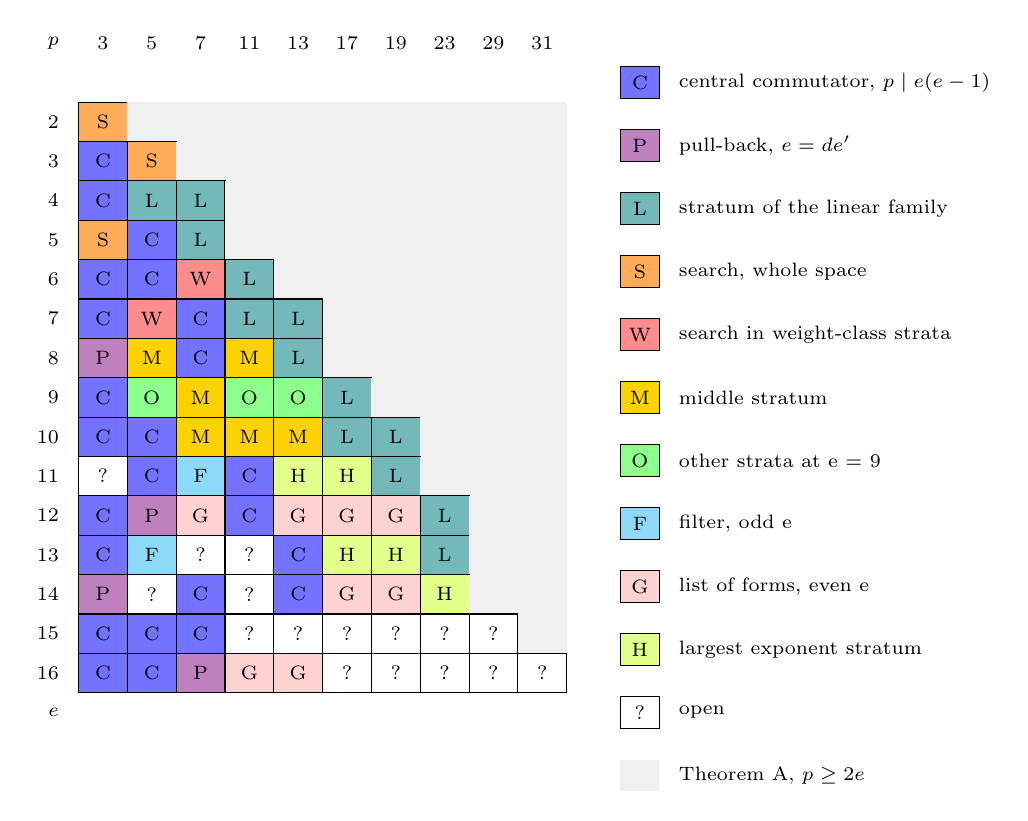
\begin{tikzpicture}[x=0.62cm,y=0.5cm,font=\scriptsize]
\node at (0,17) {3};
\node at (1,17) {5};
\node at (2,17) {7};
\node at (3,17) {11};
\node at (4,17) {13};
\node at (5,17) {17};
\node at (6,17) {19};
\node at (7,17) {23};
\node at (8,17) {29};
\node at (9,17) {31};
\node[anchor=east] at (-0.7,17) {$p$};
\node[anchor=east] at (-0.7,15) {2};
\draw[fill=orange!65] (-0.50,14.50) rectangle (0.50,15.50);
\node at (0,15) {S};
\fill[gray!12] (0.50,14.50) rectangle (1.50,15.50);
\fill[gray!12] (1.50,14.50) rectangle (2.50,15.50);
\fill[gray!12] (2.50,14.50) rectangle (3.50,15.50);
\fill[gray!12] (3.50,14.50) rectangle (4.50,15.50);
\fill[gray!12] (4.50,14.50) rectangle (5.50,15.50);
\fill[gray!12] (5.50,14.50) rectangle (6.50,15.50);
\fill[gray!12] (6.50,14.50) rectangle (7.50,15.50);
\fill[gray!12] (7.50,14.50) rectangle (8.50,15.50);
\fill[gray!12] (8.50,14.50) rectangle (9.50,15.50);
\node[anchor=east] at (-0.7,14) {3};
\draw[fill=blue!55] (-0.50,13.50) rectangle (0.50,14.50);
\node at (0,14) {C};
\draw[fill=orange!65] (0.50,13.50) rectangle (1.50,14.50);
\node at (1,14) {S};
\fill[gray!12] (1.50,13.50) rectangle (2.50,14.50);
\fill[gray!12] (2.50,13.50) rectangle (3.50,14.50);
\fill[gray!12] (3.50,13.50) rectangle (4.50,14.50);
\fill[gray!12] (4.50,13.50) rectangle (5.50,14.50);
\fill[gray!12] (5.50,13.50) rectangle (6.50,14.50);
\fill[gray!12] (6.50,13.50) rectangle (7.50,14.50);
\fill[gray!12] (7.50,13.50) rectangle (8.50,14.50);
\fill[gray!12] (8.50,13.50) rectangle (9.50,14.50);
\node[anchor=east] at (-0.7,13) {4};
\draw[fill=blue!55] (-0.50,12.50) rectangle (0.50,13.50);
\node at (0,13) {C};
\draw[fill=teal!55] (0.50,12.50) rectangle (1.50,13.50);
\node at (1,13) {L};
\draw[fill=teal!55] (1.50,12.50) rectangle (2.50,13.50);
\node at (2,13) {L};
\fill[gray!12] (2.50,12.50) rectangle (3.50,13.50);
\fill[gray!12] (3.50,12.50) rectangle (4.50,13.50);
\fill[gray!12] (4.50,12.50) rectangle (5.50,13.50);
\fill[gray!12] (5.50,12.50) rectangle (6.50,13.50);
\fill[gray!12] (6.50,12.50) rectangle (7.50,13.50);
\fill[gray!12] (7.50,12.50) rectangle (8.50,13.50);
\fill[gray!12] (8.50,12.50) rectangle (9.50,13.50);
\node[anchor=east] at (-0.7,12) {5};
\draw[fill=orange!65] (-0.50,11.50) rectangle (0.50,12.50);
\node at (0,12) {S};
\draw[fill=blue!55] (0.50,11.50) rectangle (1.50,12.50);
\node at (1,12) {C};
\draw[fill=teal!55] (1.50,11.50) rectangle (2.50,12.50);
\node at (2,12) {L};
\fill[gray!12] (2.50,11.50) rectangle (3.50,12.50);
\fill[gray!12] (3.50,11.50) rectangle (4.50,12.50);
\fill[gray!12] (4.50,11.50) rectangle (5.50,12.50);
\fill[gray!12] (5.50,11.50) rectangle (6.50,12.50);
\fill[gray!12] (6.50,11.50) rectangle (7.50,12.50);
\fill[gray!12] (7.50,11.50) rectangle (8.50,12.50);
\fill[gray!12] (8.50,11.50) rectangle (9.50,12.50);
\node[anchor=east] at (-0.7,11) {6};
\draw[fill=blue!55] (-0.50,10.50) rectangle (0.50,11.50);
\node at (0,11) {C};
\draw[fill=blue!55] (0.50,10.50) rectangle (1.50,11.50);
\node at (1,11) {C};
\draw[fill=red!45] (1.50,10.50) rectangle (2.50,11.50);
\node at (2,11) {W};
\draw[fill=teal!55] (2.50,10.50) rectangle (3.50,11.50);
\node at (3,11) {L};
\fill[gray!12] (3.50,10.50) rectangle (4.50,11.50);
\fill[gray!12] (4.50,10.50) rectangle (5.50,11.50);
\fill[gray!12] (5.50,10.50) rectangle (6.50,11.50);
\fill[gray!12] (6.50,10.50) rectangle (7.50,11.50);
\fill[gray!12] (7.50,10.50) rectangle (8.50,11.50);
\fill[gray!12] (8.50,10.50) rectangle (9.50,11.50);
\node[anchor=east] at (-0.7,10) {7};
\draw[fill=blue!55] (-0.50,9.50) rectangle (0.50,10.50);
\node at (0,10) {C};
\draw[fill=red!45] (0.50,9.50) rectangle (1.50,10.50);
\node at (1,10) {W};
\draw[fill=blue!55] (1.50,9.50) rectangle (2.50,10.50);
\node at (2,10) {C};
\draw[fill=teal!55] (2.50,9.50) rectangle (3.50,10.50);
\node at (3,10) {L};
\draw[fill=teal!55] (3.50,9.50) rectangle (4.50,10.50);
\node at (4,10) {L};
\fill[gray!12] (4.50,9.50) rectangle (5.50,10.50);
\fill[gray!12] (5.50,9.50) rectangle (6.50,10.50);
\fill[gray!12] (6.50,9.50) rectangle (7.50,10.50);
\fill[gray!12] (7.50,9.50) rectangle (8.50,10.50);
\fill[gray!12] (8.50,9.50) rectangle (9.50,10.50);
\node[anchor=east] at (-0.7,9) {8};
\draw[fill=violet!50] (-0.50,8.50) rectangle (0.50,9.50);
\node at (0,9) {P};
\draw[fill=yellow!70!orange] (0.50,8.50) rectangle (1.50,9.50);
\node at (1,9) {M};
\draw[fill=blue!55] (1.50,8.50) rectangle (2.50,9.50);
\node at (2,9) {C};
\draw[fill=yellow!70!orange] (2.50,8.50) rectangle (3.50,9.50);
\node at (3,9) {M};
\draw[fill=teal!55] (3.50,8.50) rectangle (4.50,9.50);
\node at (4,9) {L};
\fill[gray!12] (4.50,8.50) rectangle (5.50,9.50);
\fill[gray!12] (5.50,8.50) rectangle (6.50,9.50);
\fill[gray!12] (6.50,8.50) rectangle (7.50,9.50);
\fill[gray!12] (7.50,8.50) rectangle (8.50,9.50);
\fill[gray!12] (8.50,8.50) rectangle (9.50,9.50);
\node[anchor=east] at (-0.7,8) {9};
\draw[fill=blue!55] (-0.50,7.50) rectangle (0.50,8.50);
\node at (0,8) {C};
\draw[fill=green!45] (0.50,7.50) rectangle (1.50,8.50);
\node at (1,8) {O};
\draw[fill=yellow!70!orange] (1.50,7.50) rectangle (2.50,8.50);
\node at (2,8) {M};
\draw[fill=green!45] (2.50,7.50) rectangle (3.50,8.50);
\node at (3,8) {O};
\draw[fill=green!45] (3.50,7.50) rectangle (4.50,8.50);
\node at (4,8) {O};
\draw[fill=teal!55] (4.50,7.50) rectangle (5.50,8.50);
\node at (5,8) {L};
\fill[gray!12] (5.50,7.50) rectangle (6.50,8.50);
\fill[gray!12] (6.50,7.50) rectangle (7.50,8.50);
\fill[gray!12] (7.50,7.50) rectangle (8.50,8.50);
\fill[gray!12] (8.50,7.50) rectangle (9.50,8.50);
\node[anchor=east] at (-0.7,7) {10};
\draw[fill=blue!55] (-0.50,6.50) rectangle (0.50,7.50);
\node at (0,7) {C};
\draw[fill=blue!55] (0.50,6.50) rectangle (1.50,7.50);
\node at (1,7) {C};
\draw[fill=yellow!70!orange] (1.50,6.50) rectangle (2.50,7.50);
\node at (2,7) {M};
\draw[fill=yellow!70!orange] (2.50,6.50) rectangle (3.50,7.50);
\node at (3,7) {M};
\draw[fill=yellow!70!orange] (3.50,6.50) rectangle (4.50,7.50);
\node at (4,7) {M};
\draw[fill=teal!55] (4.50,6.50) rectangle (5.50,7.50);
\node at (5,7) {L};
\draw[fill=teal!55] (5.50,6.50) rectangle (6.50,7.50);
\node at (6,7) {L};
\fill[gray!12] (6.50,6.50) rectangle (7.50,7.50);
\fill[gray!12] (7.50,6.50) rectangle (8.50,7.50);
\fill[gray!12] (8.50,6.50) rectangle (9.50,7.50);
\node[anchor=east] at (-0.7,6) {11};
\draw[fill=white] (-0.50,5.50) rectangle (0.50,6.50);
\node at (0,6) {?};
\draw[fill=blue!55] (0.50,5.50) rectangle (1.50,6.50);
\node at (1,6) {C};
\draw[fill=cyan!45] (1.50,5.50) rectangle (2.50,6.50);
\node at (2,6) {F};
\draw[fill=blue!55] (2.50,5.50) rectangle (3.50,6.50);
\node at (3,6) {C};
\draw[fill=lime!45] (3.50,5.50) rectangle (4.50,6.50);
\node at (4,6) {H};
\draw[fill=lime!45] (4.50,5.50) rectangle (5.50,6.50);
\node at (5,6) {H};
\draw[fill=teal!55] (5.50,5.50) rectangle (6.50,6.50);
\node at (6,6) {L};
\fill[gray!12] (6.50,5.50) rectangle (7.50,6.50);
\fill[gray!12] (7.50,5.50) rectangle (8.50,6.50);
\fill[gray!12] (8.50,5.50) rectangle (9.50,6.50);
\node[anchor=east] at (-0.7,5) {12};
\draw[fill=blue!55] (-0.50,4.50) rectangle (0.50,5.50);
\node at (0,5) {C};
\draw[fill=violet!50] (0.50,4.50) rectangle (1.50,5.50);
\node at (1,5) {P};
\draw[fill=pink!70] (1.50,4.50) rectangle (2.50,5.50);
\node at (2,5) {G};
\draw[fill=blue!55] (2.50,4.50) rectangle (3.50,5.50);
\node at (3,5) {C};
\draw[fill=pink!70] (3.50,4.50) rectangle (4.50,5.50);
\node at (4,5) {G};
\draw[fill=pink!70] (4.50,4.50) rectangle (5.50,5.50);
\node at (5,5) {G};
\draw[fill=pink!70] (5.50,4.50) rectangle (6.50,5.50);
\node at (6,5) {G};
\draw[fill=teal!55] (6.50,4.50) rectangle (7.50,5.50);
\node at (7,5) {L};
\fill[gray!12] (7.50,4.50) rectangle (8.50,5.50);
\fill[gray!12] (8.50,4.50) rectangle (9.50,5.50);
\node[anchor=east] at (-0.7,4) {13};
\draw[fill=blue!55] (-0.50,3.50) rectangle (0.50,4.50);
\node at (0,4) {C};
\draw[fill=cyan!45] (0.50,3.50) rectangle (1.50,4.50);
\node at (1,4) {F};
\draw[fill=white] (1.50,3.50) rectangle (2.50,4.50);
\node at (2,4) {?};
\draw[fill=white] (2.50,3.50) rectangle (3.50,4.50);
\node at (3,4) {?};
\draw[fill=blue!55] (3.50,3.50) rectangle (4.50,4.50);
\node at (4,4) {C};
\draw[fill=lime!45] (4.50,3.50) rectangle (5.50,4.50);
\node at (5,4) {H};
\draw[fill=lime!45] (5.50,3.50) rectangle (6.50,4.50);
\node at (6,4) {H};
\draw[fill=teal!55] (6.50,3.50) rectangle (7.50,4.50);
\node at (7,4) {L};
\fill[gray!12] (7.50,3.50) rectangle (8.50,4.50);
\fill[gray!12] (8.50,3.50) rectangle (9.50,4.50);
\node[anchor=east] at (-0.7,3) {14};
\draw[fill=violet!50] (-0.50,2.50) rectangle (0.50,3.50);
\node at (0,3) {P};
\draw[fill=white] (0.50,2.50) rectangle (1.50,3.50);
\node at (1,3) {?};
\draw[fill=blue!55] (1.50,2.50) rectangle (2.50,3.50);
\node at (2,3) {C};
\draw[fill=white] (2.50,2.50) rectangle (3.50,3.50);
\node at (3,3) {?};
\draw[fill=blue!55] (3.50,2.50) rectangle (4.50,3.50);
\node at (4,3) {C};
\draw[fill=pink!70] (4.50,2.50) rectangle (5.50,3.50);
\node at (5,3) {G};
\draw[fill=pink!70] (5.50,2.50) rectangle (6.50,3.50);
\node at (6,3) {G};
\draw[fill=lime!45] (6.50,2.50) rectangle (7.50,3.50);
\node at (7,3) {H};
\fill[gray!12] (7.50,2.50) rectangle (8.50,3.50);
\fill[gray!12] (8.50,2.50) rectangle (9.50,3.50);
\node[anchor=east] at (-0.7,2) {15};
\draw[fill=blue!55] (-0.50,1.50) rectangle (0.50,2.50);
\node at (0,2) {C};
\draw[fill=blue!55] (0.50,1.50) rectangle (1.50,2.50);
\node at (1,2) {C};
\draw[fill=blue!55] (1.50,1.50) rectangle (2.50,2.50);
\node at (2,2) {C};
\draw[fill=white] (2.50,1.50) rectangle (3.50,2.50);
\node at (3,2) {?};
\draw[fill=white] (3.50,1.50) rectangle (4.50,2.50);
\node at (4,2) {?};
\draw[fill=white] (4.50,1.50) rectangle (5.50,2.50);
\node at (5,2) {?};
\draw[fill=white] (5.50,1.50) rectangle (6.50,2.50);
\node at (6,2) {?};
\draw[fill=white] (6.50,1.50) rectangle (7.50,2.50);
\node at (7,2) {?};
\draw[fill=white] (7.50,1.50) rectangle (8.50,2.50);
\node at (8,2) {?};
\fill[gray!12] (8.50,1.50) rectangle (9.50,2.50);
\node[anchor=east] at (-0.7,1) {16};
\draw[fill=blue!55] (-0.50,0.50) rectangle (0.50,1.50);
\node at (0,1) {C};
\draw[fill=blue!55] (0.50,0.50) rectangle (1.50,1.50);
\node at (1,1) {C};
\draw[fill=violet!50] (1.50,0.50) rectangle (2.50,1.50);
\node at (2,1) {P};
\draw[fill=pink!70] (2.50,0.50) rectangle (3.50,1.50);
\node at (3,1) {G};
\draw[fill=pink!70] (3.50,0.50) rectangle (4.50,1.50);
\node at (4,1) {G};
\draw[fill=white] (4.50,0.50) rectangle (5.50,1.50);
\node at (5,1) {?};
\draw[fill=white] (5.50,0.50) rectangle (6.50,1.50);
\node at (6,1) {?};
\draw[fill=white] (6.50,0.50) rectangle (7.50,1.50);
\node at (7,1) {?};
\draw[fill=white] (7.50,0.50) rectangle (8.50,1.50);
\node at (8,1) {?};
\draw[fill=white] (8.50,0.50) rectangle (9.50,1.50);
\node at (9,1) {?};
\node[anchor=east] at (-0.7,0) {$e$};
\draw[fill=blue!55] (10.60,15.60) rectangle (11.40,16.40);
\node at (11.00,16.00) {C};
\node[anchor=west] at (11.60,16.00) {central commutator, $p\mid e(e-1)$};
\draw[fill=violet!50] (10.60,14.00) rectangle (11.40,14.80);
\node at (11.00,14.40) {P};
\node[anchor=west] at (11.60,14.40) {pull-back, $e=de'$};
\draw[fill=teal!55] (10.60,12.40) rectangle (11.40,13.20);
\node at (11.00,12.80) {L};
\node[anchor=west] at (11.60,12.80) {stratum of the linear family};
\draw[fill=orange!65] (10.60,10.80) rectangle (11.40,11.60);
\node at (11.00,11.20) {S};
\node[anchor=west] at (11.60,11.20) {search, whole space};
\draw[fill=red!45] (10.60,9.20) rectangle (11.40,10.00);
\node at (11.00,9.60) {W};
\node[anchor=west] at (11.60,9.60) {search in weight-class strata};
\draw[fill=yellow!70!orange] (10.60,7.60) rectangle (11.40,8.40);
\node at (11.00,8.00) {M};
\node[anchor=west] at (11.60,8.00) {middle stratum};
\draw[fill=green!45] (10.60,6.00) rectangle (11.40,6.80);
\node at (11.00,6.40) {O};
\node[anchor=west] at (11.60,6.40) {other strata at e = 9};
\draw[fill=cyan!45] (10.60,4.40) rectangle (11.40,5.20);
\node at (11.00,4.80) {F};
\node[anchor=west] at (11.60,4.80) {filter, odd e};
\draw[fill=pink!70] (10.60,2.80) rectangle (11.40,3.60);
\node at (11.00,3.20) {G};
\node[anchor=west] at (11.60,3.20) {list of forms, even e};
\draw[fill=lime!45] (10.60,1.20) rectangle (11.40,2.00);
\node at (11.00,1.60) {H};
\node[anchor=west] at (11.60,1.60) {largest exponent stratum};
\draw[fill=white] (10.60,-0.40) rectangle (11.40,0.40);
\node at (11.00,0.00) {?};
\node[anchor=west] at (11.60,0.00) {open};
\fill[gray!12] (10.60,-2.00) rectangle (11.40,-1.20);
\node[anchor=west] at (11.60,-1.60) {Theorem A, $p\ge2e$};
\end{tikzpicture}

\caption{The pairs $(e,p)$ with $p$ an odd prime, for $2\le e\le16$ (rows) and $p<2e$ (columns, coloured cells); grey cells are $p\ge2e$ (Theorem~\ref{thm:A}). Each coloured cell carries the code of the first case that settles it: C, $p$ divides $e(e-1)$; P, the pull-back; L, a pure member of the linear family; S, a pair found by search in the whole space; W, a pair found by the search in the weight-class strata; M, a pair found in the middle stratum; O, a pair found in the other strata at $e=9$ (Section~\ref{sec:reslinrule}); F, a pair found through the filter of Section~\ref{sec:resfilter}; G, a pair found through a list of forms (Section~\ref{sec:reslists}); H, a pair found in the stratum with the largest exponent (Section~\ref{sec:reslargest}); the cells marked $?$ are open. The cells are computed by the script of the paper from the stored results of the searches and of the linear family and from Corollaries~\ref{cor:cases} and~\ref{cor:scale1}; the pairs of the codes L, S, W, M, O, F, G and H are pairs over $\F_p$.}
\label{fig:grid}
\end{figure}

Figure~\ref{fig:grid} shows that the cells settled by the central commutator follow the divisors of $e(e-1)$, that the pull-back adds a few cells in the lower rows (for example $(12,5)$, $(14,3)$, $(16,7)$), that the searches add cells up to $e=10$ and a few at larger $e$, and that the open cells do not stop at any $e$: the open cells are the primes that divide neither $e(e-1)$ nor a factor $d$ of $e$ and that no search has reached. It does not show whether the open pairs are realized.

\subsection{Consequences: the rays with \texorpdfstring{$d_3=10$}{d3=10} and the rays with \texorpdfstring{$d_3\le9$}{d3<=9}}
\label{sec:consequences}

\begin{proposition}\label{prop:least}
Over every field, the primitive points $(1,3,8,6)$ on $(0,4,9,10)$ and $(6,8,3,1)$ on $(0,1,6,10)$ are the Betti table of no finitely generated graded module over $S$, and no multiple $m\ge1$ of either is the Betti table of a finitely generated graded module over $U$.
\end{proposition}
\begin{proof}
\emph{Over $S$.} For $(1,3,8,6)$ on $(0,4,9,10)$: $a=1$, $b=3$, codimension $3$. The second syzygy bound is violated, since $d_2=9>2\cdot4=8$. The codimension obstruction holds with equality ($3=3+1-1$), so the table would be that of the Buchsbaum--Rim complex of a $1\times3$ map of quartics, which is the Koszul table $(1,3,3,1)$ on $(0,4,8,12)$, not this one. Independently, $M=S/I$ with $I$ minimally generated by three quartics of height $3$ (finite length), and in the Cohen--Macaulay ring $S$ three elements generating an ideal of height $3$ form a regular sequence, so the resolution is the Koszul complex on $(0,4,8,12)$. For $(6,8,3,1)$ on $(0,1,6,10)$: the codimension obstruction holds with equality ($8=3+6-1$) and the Buchsbaum--Rim complex of a $6\times8$ linear map has the table $(6,8,8,6)$ on $(0,1,7,8)$, not $(6,8,3,1)$ on $(0,1,6,10)$; moreover $d_3=10$ exceeds the sum of the eight largest relation degrees, $8$, so the regularity bound is violated. This second example is Erman's own example of the equality case~\cite[Proposition~3.1 and the discussion that follows]{Erman09}, and the first is its rotation by the duality of Remark~3.2 there; all arguments are valid over any field.

\emph{Finite length is automatic.} A pure table on the ray satisfies~\eqref{eq:HK}, so $p_\beta(t)=(1-t)^3q(t)$ with $q$ a polynomial and every module with this table over $S$ has Hilbert series $q(t)$, a polynomial.

\emph{Over $U$.} A finitely generated graded module $N$ with Betti table $m\beta$ has $\Hilb_N(t)=m\,p_\beta(t)/((1-t)^2(1-t^2))=m\,q(t)/(1+t)$ by Lemma~\ref{lem:parity}, with $q(-1)=p_\beta(-1)/8$. Here $p_\beta(-1)=-16$ and $16$, so $q(-1)=\mp2\neq0$. Writing $m\,q(t)/(1+t)=s(t)+m\,q(-1)/(1+t)$ with $s$ a polynomial, the coefficient of $t^n$ is $m\,q(-1)(-1)^n$ for $n>\deg s$, negative for half of all large $n$, which is impossible for a Hilbert function. So no finitely generated graded $U$-module of any length has such a table.
\end{proof}

\begin{remark}
The finite length hypothesis is not needed for either half: over $S$ every module with such a table has finite length, and over $U$ no module of any length has it. The exclusion over $S$ is in print as an instance of the obstructions of Erman; the half over $U$ is the parity test of Jiang, Li, Sun, Wang, Xiao and Yu applied to these two rays. The two rays have $d_3=10$, whereas the example of~\cite{JLSWXY} has $d_3=21$.
\end{remark}

\begin{proposition}\label{prop:lownine}
Let $k$ be a field of characteristic $0$. Every integral point on a pure ray with $d_3-d_0\le9$ is the Betti table of a finite length graded module over $S\otimes k$ or over $U\otimes k$.
\end{proposition}
\begin{proof}[Evidence]
Every integral point on a pure ray is $m\beta_d$ with $m\ge1$, and the direct sum of $m$ copies of a realization of $\beta_d$ realizes it over the same ring; so it suffices to realize the primitive point of each of the $84=\binom93$ degree sequences with $0<d_1<d_2<d_3\le9$. The evidence for the primitive points is of five types (Table~\ref{tab:lownine}):
\begin{enumerate}
\item for \nlowNineFormula{} rays, a formula whose number of generators equals $\beta_0$: Eisenbud--Schreyer (Theorem~5.1, any field), Eisenbud--Fl{\o}ystad--Weyman (characteristic $0$), the Koszul complex, $S/\mathfrak m^a$ and its dual, Buchsbaum--Rim complexes and generic Pfaffians [V for the theorems; MV for the numbers of generators, which agree between the Python census and Macaulay2 on all \nrays{} rays];
\item for \nlowNineScaling{} rays, the scaling of a formula ray (Section~\ref{sec:realizability}) [D];
\item for \nlowNineSocle{} and \nlowNineModule{} rays, an explicit module over $\Q$, the image of an integer matrix inside a truncated ring or the cokernel of an integer matrix, whose Betti table over $\Q$ was computed in Macaulay2 and recomputed in Singular, with the length equal to the Herzog--K\"uhl length [MV];
\item for \nlowNineDual{} rays, the $\Ext^3$ dual of a module of the previous type, by the duality of Section~\ref{sec:realizability} [D], with the table of the dual computed over $\Q$ on \nqqDualsDirect{} of them [MV];
\item for the five rays $(0,1,3,4)$, $(0,1,5,6)$, $(0,1,7,8)$, $(0,2,6,8)$ and $(0,3,5,8)$ that are excluded over $S$ and pass the parity test, an explicit module over $U$ (Table~\ref{tab:ten}) [MV].
\end{enumerate}
Base change from $\Q$ to $k$ preserves Betti tables and finite length. These \nlowNineExcluded{} rays are the only rays with $d_3\le9$ excluded over $S$. \qedhere
\end{proof}
\FloatBarrier
\section{Experimental design}
\label{sec:expdesign}

The computations behind the paper are archived in the repository under the identifiers \EXP{001}, \EXP{002}, \EXP{003}, \EXP{004}, \EXP{005}, \EXP{006}, \EXP{007}, \EXP{008}, \EXP{009}, \EXP{010}, \EXP{011}, \EXP{012}, \EXP{013}, \EXP{014}, \EXP{015}, \EXP{016}, \EXP{017} and \EXP{018}; these identifiers denote the archived computations and are used only as references to them. \EXP{001} is the census over $S$ of the \nrays{} pure rays with $d_3\le12$, with the formula constructions, the obstructions, the search and the rechecks. \EXP{002} is the study of the primitive points over $U$ on the rays that pass the parity test and are excluded over $S$, with the calibration on the Kostant modules and on the family $M_e$. \EXP{003} is the study of $U$ in characteristic $2$, of the proof steps of Theorem~A for $e\le8$, and of the genericity of the pair $(x^e,y^e)$. \EXP{004} computes the rank certificates of Section~\ref{sec:rank} on the \nfourHits{} verified hits of \EXP{001} and resolves the two disputed modules over $\Q$ in Singular. \EXP{005} archives the machine checks of the characteristic $2$ theorem and of the family $M_e$ for $e=6,7$ (\nfiveCasesAll{} presentations over $\F_2$, $\F_4$ and $\F_{16}$ and the $24$ modules $M_e$ over $\Q$ and the primes up to $31$). \EXP{006} searches for pure pairs of forms in odd characteristic below $2e$, in the families of Section~\ref{sec:pairsearch}. \EXP{007} computes the tangent space of the rank locus at $W_0$, tests five explicit pairs over the rationals, a linear family, a plane section and the common-factor locus (Section~\ref{sec:tangentmethods}). \EXP{008} extends the search of \EXP{006} to quintics over $\F_5$ and $\F_7$ and to sextics over $\F_3$, with an early stop.

\subsection{Questions and predictions stated before the computations}

Each computation poses its questions and states its predictions, with the probability the author assigned to each, in a file committed to the repository before the first run of that computation. The questions are: for every ray with $d_3\le12$, is the primitive point realized, excluded or open over $S$, and what is the least multiple $c_d$ (\EXP{001}); is the primitive point of each of the ten rays realized over $U$, and is $M_e$ pure for $e\le6$ (\EXP{002}); in characteristic $2$ does any pair of quadrics have a finite length quotient, which of the other nine rays are realized, do the intermediate statements of the proof of Theorem~A hold for $e\le8$ and for which primes is $M_e$ pure, and is a general pair of forms of degree $e$ pure (\EXP{003}); does the rank test pass on the hits without a completed rational recheck (\EXP{004}). The predictions include: the stage-0 count of realized primitive points between $52$ and $56$ and exactly $12$ excluded (probability $0.85$); persistence over $\Q$ of every prime-field hit ($0.85$ per hit); $M_e$ pure for $e=3$ ($0.8$) and for $e=4,5,6$ ($0.7$ each); at least $9$ of $10$ random $2\times3$ matrices of quadrics giving the table $(2,3,3,2)$ ($0.6$); no pair of quadrics of finite length over $\F_{2^r}$ ($0.95$); the set of primes at which $M_e$ is not pure contained in the set predicted from factorials and tableau counts ($0.75$); a non-pure table for a general pair of forms with $e=4,5,10$ ($0.85$); and, for \EXP{004}, the rank test passing on at least $55$ of the $66$ hits without a completed positive rational recheck ($0.75$) and failing on the two hits whose rational recheck had been recorded as failed ($0.5$).

The predictions of the four later computations were fixed in the same way. For \EXP{005}: no presentation with $b\le a+1$ in characteristic $2$ has finite length; every such presentation whose Hilbert function becomes constant has the value $\tfrac{a(a+1)}2L\cdot L$ of Table~\ref{tab:eventual}, none is unclassified, at most $5$ percent of the random cases over $\F_{16}$ grow and every single cubic grows; with $b=a+2$ at least $8$ of $10$ random presentations of each of four shapes have finite length; and $M_e$ has the pure table for $e=6,7$ exactly over $\Q$ and the primes at least $2e$. For \EXP{006}: pure pairs of cubics exist over $\F_3$ and $\F_5$ and at least half of the random pairs over $\F_{25}$ and $\F_{27}$ are pure (confidence $0.85$ for characteristic $5$, $0.7$ for characteristic $3$); the share of random quartic spaces with $\operatorname{rank}\mu_{12}\le48$ lies between $0.3q^{-2}$ and $3q^{-2}$ in each of six fields ($0.7$); pure pairs of quartics exist over $\F_3$, $\F_5$ and $\F_7$ ($0.6$ for each prime); and over $\F_{11}$ and $\F_{13}$ pure pairs exist outside the orbit of $W_0$ ($0.75$). For \EXP{007}: the tangent dimensions, the explicit pairs, the linear family, the plane section and the common-factor locus take the values that Section~\ref{sec:resfamily} reports, with no confidence stated; a tangent dimension above $4e-4$, a pair that is not pure or lies in the orbit, or a member of the linear family outside $D_e$ would have contradicted the corresponding statement. For \EXP{008}: pure pairs of quintics exist over $\F_5$ (confidence $0.8$) and over $\F_7$ ($0.75$), and pure pairs of sextics exist over $\F_3$ ($0.5$), each found in a random search of $\neightAFivePlanned$, $\neightBSevenPlanned$ and $\neightCThreePlanned$ spaces with the rank filter first; a family that ends without a pure space would say only that the share of pure spaces over that field is small, and not that none exists. Section~\ref{sec:predfail} reports which predictions failed.

Three later computations extend the archive: \EXP{009}, \EXP{011} and \EXP{012}. \EXP{009} enumerates the four-parameter linear family $L_e$ over $\F_p$ for the fifteen pairs $(e,p)$ with $4\le e\le7$, $p$ odd and $p<2e$, with five control pairs where Proposition~\ref{prop:linear} applies, and samples it over $\F_{p^2}$ in the nine pairs where the enumeration finds no pure member (Section~\ref{sec:lfmethods}). \EXP{011} checks Theorem~\ref{thm:central} on sixteen pairs, among them $(7,7)$, which no earlier computation had reached, and $(9,3)$, $(11,11)$, $(13,13)$, $(15,3)$ and $(15,5)$, and counts what happens on five pairs outside its hypotheses. \EXP{012} checks the explicit pairs of Corollary~\ref{cor:cases} on eleven cases, among them $(6,5)$ and $(7,3)$, and the equivalence of Theorem~\ref{thm:crit} on $1{,}600$ random pairs of the class, and counts what happens on three pairs built to violate the criterion (Section~\ref{sec:critmethods}). The predictions were fixed in the same way as for the earlier computations, each in a file committed before the computation. For \EXP{009}: no member of $L_e$ over $\F_p$ has $\operatorname{rank}\mu_{3e}>r$ in any of the fifteen pairs below $2e$ (confidence $0.7$); in each of the pairs $(4,5)$, $(4,7)$, $(5,7)$, $(6,7)$, $(6,11)$, $(7,11)$ and $(7,13)$ the family has a pure member over $\F_p$ (confidence $0.55$ for each); and in each of the pairs $(4,3)$, $(5,3)$, $(5,5)$, $(6,3)$, $(6,5)$, $(7,3)$, $(7,5)$ and $(7,7)$ a pure member exists over $\F_p$ or $\F_{p^2}$ (confidence $0.3$ for each). For \EXP{011}: in every case of the two families inside the hypotheses the identities hold, the Hilbert function is $h_e$, the length is $e^3$ and every Betti table computed is $(1,2,2,1)$ (confidence $0.97$); the pairs outside the hypotheses with $l_1=0$, with $l_1,l_2$ dependent and with common factor are not pure ($0.9$), and the two pairs with $p\nmid e$ do not have the pure Hilbert function ($0.8$). For \EXP{012}: in every explicit case the identities hold, the criterion holds, the Hilbert function is $h_e$, the length is $e^3$ and the table is pure ($0.93$); on every random pair the identity holds and the criterion holds exactly when the pair has the pure Hilbert function, with every computed table pure ($0.9$); and on the three pairs built to violate the criterion it fails and the module is not of finite length ($0.9$). Section~\ref{sec:predfail} reports which predictions failed.

The second set of later computations is \EXP{010}, \EXP{013} and \EXP{014}. \EXP{010} searches the weight-class strata of Section~\ref{sec:strata} in the five pairs $(6,5)$, $(6,7)$, $(7,3)$, $(7,5)$, $(7,7)$ that remained open after the linear family, in nine settled pairs as controls, and, exploratory, at $e=8$ (Section~\ref{sec:strsearch}). \EXP{013} computes the pull-backs of Theorem~\ref{thm:scale} on ten cases and two cases outside its hypotheses (Section~\ref{sec:pbmethods}). \EXP{014} searches the middle stratum $S(e;0,e/2)$ at $e=8$, $10$ and $12$ and two strata at $e=9$. The predictions of each were fixed in a file committed before the computation. For \EXP{010}: an admissible stratum holds a pure member over $\F_p$ in each of the five open pairs (confidence $0.8$, $0.75$, $0.7$, $0.65$, $0.55$ at $(6,5)$, $(6,7)$, $(7,3)$, $(7,5)$, $(7,7)$); the share of members with the pure Hilbert function in $S(2;0,1)$ is between $0.1$ and $1.5$ times $p^{-h_e(3e)}$ in every pair where it is positive ($0.6$); no member of a stratum that is not admissible has the pure Hilbert function ($0.97$); no member of a stratum with $p$ dividing $m$ has the rank $r$ ($0.7$); and at $e=8$ the stratum $S(7;0,1)$ holds a pure member at $(8,11)$ and at $(8,13)$ ($0.6$ each), a pure member is found at $(8,3)$ ($0.5$), at $(8,5)$ ($0.3$) and at $(8,7)$ ($0.3$). For \EXP{013}: in the ten cases the table of the pull-back is the table of $M'$ with the degrees multiplied by $d$ and the length is $d^3$ times that of $M'$ ($0.9$ for the pairs), and the pull-back along the $p$-th power map is not pure ($0.95$). For \EXP{014}: the middle stratum holds a pure member at $e=8$ ($0.6$ each for $p=3,5,7,11,13$) and at $e=10$ and $12$ ($0.5$ each); no member of the stratum has the rank $r$ at $(10,5)$ ($0.7$); the stratum $S(5;0,4)$ at $e=9$ holds a pure member at $p=7,11,13$ ($0.5$ each) and no member of rank $r$ at $p=5$ ($0.7$); and $S(8;0,1)$ at $e=9$ holds a pure member at $p=17$ and none at $p=11$ and $13$ ($0.6$ together). Section~\ref{sec:predfail} reports which predictions failed.

The third set is \EXP{015} and \EXP{017}, each with its questions and predictions committed before the first run. \EXP{015} asks whether the stratum of the linear family holds pure members exactly when $2e-p\le3$ at the twelve pairs $e=10$ to $13$ (prediction P1, all twelve outcomes), whether the three open pairs at $e=9$ have a pure pair in some stratum (prediction P2), and records, before the results were read, the predictions that follow from Corollary~\ref{cor:wzstrata} for the strata at $e=9$. \EXP{017} asks whether the filter of Section~\ref{sec:resfilter} leads to pure pairs at $(9,11)$ and $(9,13)$ (predictions P1 to P4, of which P1 concerns the share of members that pass). The acceptance criteria are those of the first set: pure Hilbert function and Betti table computed in $U$ by two instruments on the first members. \EXP{016} asks whether the lists of forms $\Gamma$ with (C) and the congruence of Theorem~\ref{thm:cong} are not empty at fourteen pairs not settled before, with the five predictions recorded before the first run on such a pair (Section~\ref{sec:reslists}). \EXP{018} asks whether the stratum with the largest exponent allowed by Corollary~\ref{cor:wzstrata} holds a pure pair at five open pairs and whether the stratum with the next exponent holds none (three predictions, Section~\ref{sec:reslargest}).

\subsection{Known-answer checks, instruments and their independence}

Before any claim, each computation reproduces known answers. For \EXP{001} these are \ngateThreeEach{} known answers, documented in the Macaulay2 package or in the literature, all reproduced over $\mathbb{Z}/101$, $\F_{32003}$ and $\Q$, and the values $(1,3,8,6)$ and $(6,8,3,1)$ with parities $-16$ and $16$ on the two rays with $d_3=10$. For \EXP{002} and \EXP{003} these are the trivial module, $U/U(x^2,y^2,xy+yx)$ and the Kostant modules: \ncalibModules{} modules in the first computation and \nthreeCalib{} cases (several fields) in the second, with known tables. The instruments are independent in code and in method. The first is the exact library of the repository (\texttt{uhlib}): the algebra $U$, quotient modules degree by degree, the Tor complex of Section~\ref{sec:tor}, over $\Q$, $\F_p$ and $\F_{2^r}$ with a verified irreducible modulus. The second is Singular 4.3.2 with Plural, reading the Betti table from the generators of each syzygy module. The census has two implementations, in Python with rational arithmetic and in Macaulay2, compared on all \nrays{} rays; the search uses the Macaulay2 package~\cite{M2BS}; the rechecks use a fresh process, Singular, and the rational lift (Section~\ref{sec:search}). A claim over $U$ is accepted only when both instruments agree. The later computations reproduce known answers in the same way. \EXP{005} reproduces the Hilbert functions of the \nfiveGOneCompared{} pairs of quadrics over $\F_2$ stored by \EXP{003} and agrees with a second code path of the library on \nfiveGTwoCompared{} random presentations over $\F_2$, $\F_4$, $\F_{16}$ and $\F_{32003}$. \EXP{006} reproduces that $(x^4,y^4)$ is pure over $\F_{11}$ and $\F_{13}$ and not over $\F_3$, $\F_5$ and $\F_7$, that $(x^3,y^3)$ is pure over $\F_7$ and not over $\F_3$ and $\F_5$, and the pure table on $(0,2,6,8)$ of the pair of quadrics over $\F_3$ of \EXP{003}. \EXP{007} reproduces the purity of $W_0$ for $e=4,\dots,7$ and the dimensions of the generic determinantal varieties. \EXP{008} rebuilds three pure spaces of \EXP{006} at $e=5$, reproduces that $\langle x^5,y^5\rangle$ is pure over $\F_{11}$ and not over $\F_5$ and $\F_7$, that $\langle x^6,y^6\rangle$ is pure over $\F_{13}$ and not over $\F_3$, and the stored counts on the first $2{,}000$ quintic spaces of \EXP{006} (\neightGOneCases{} known answers). Singular gives the same table or Hilbert function as the library on \nfiveGThreeAgree{} of \nfiveGThreeCompared{} sampled cases of \EXP{005}, on \nsixSingularSample{} of \nsixSingularSample{} pure spaces of \EXP{006}, on the \nsevenGThreeSpaces{} spaces of \EXP{007} and on \neightSingularSample{} of \neightSingularSample{} pure spaces of \EXP{008}. For the searches of \EXP{006} and \EXP{008} the counts of pure spaces rest on the first instrument alone, and Singular confirms a fixed sample of \nsixSingularSample{} and \neightSingularSample{} pure spaces.

The three later computations reproduce known answers. \EXP{009} reproduces that $L_4(0,0,0,0)=\langle x^4,y^4\rangle$ is pure over $\F_{11}$ and $\F_{13}$ and not over $\F_3$, $\F_5$ and $\F_7$, that $L_4(1,0,0,0)$ is pure over $\F_{13}$, and, in the control pairs, that no member has rank above $r$ and at least half of the members of rank $r$ examined are pure; Singular gives the pure table on the first five pure members of each of the eleven pairs with a pure member ($55$ of $55$), from scripts generated from the stored polynomials, and $10$ unit tests cover the family constructor against the printed polynomials, the enumeration, the rank routine at $e=6,7$ against the module construction of the library on five members per field, and the stopping rule. \EXP{011} reproduces that $\langle x^5,y^5\rangle$ is pure over $\F_{11}$ and not over $\F_5$ and that $\langle x^5+yz^2,y^5+xz^2\rangle$ over $\F_5$ has the pure table, with Singular agreeing with the library on all $16$ cases and $6$ unit tests. \EXP{012} reproduces that $\langle x^4+z^2,y^4+z^2\rangle$ over $\F_3$ and $\langle x^5+yz^2,y^5+xz^2\rangle$ over $\F_5$ are pure and $\langle x^4,y^4\rangle$ over $\F_5$ is not of finite length within the degree bound, and that the criterion routine returns true on $(z^3,X^2+z^3,Y^2+z^3)$ and false on $(zXY,X^2,Y^2+z^3)$ over $\F_3$; Singular agrees with the library on all $11$ explicit cases, and $9$ unit tests cover the basis of $V_e$ for $(4,3)$ and $(6,3)$, the passage from $(A,\beta_1,\beta_2)$ to the polynomial of $U$, the quantities $n(f)$ and $D$, the identity $gf-fg=-Dz$ and the criterion routine.

The second set reproduces known answers. \EXP{010} reproduces before the families that the power pairs are pure over $\F_{13}$ for $e=4,5,6$ and over $\F_{17}$ for $e=7$ and that $\langle x^4,y^4\rangle$ is not pure over $\F_5$, that the two pure pairs of \EXP{009} over $\F_{11}$ and $\F_{13}$ are pure and lie in $S(5;0,1)$ and $S(6;0,1)$, that the rank routine agrees with the module construction of the library on $200$ random pairs in four degrees, and that the admissible strata number $17$, $19$, $34$, $34$, $58$ for $e=4,\dots,8$; after the controls it reproduces the pure members and the absence of the pure Hilbert function in $S(4;0,1)$ at $(5,5)$ and the pure members at $(5,7)$, $(6,3)$, $(6,11)$, $(7,11)$, $(7,13)$; Singular gives the same pure table on $114$ of $114$ members and $10$ unit tests cover the weights, the supports, the enumeration, the admissible list for $e=5$, the rank routine and the early stop. \EXP{013} reproduces that the five pairs whose images under the endomorphisms are taken are pure with central commutator, that the modules of the other families have the lengths stated, and that Singular and the library give the same table on all $20$ modules ($9$ unit tests, among them $\varphi(uv)=\varphi(u)\varphi(v)$ on random forms). \EXP{014} reproduces that $f=x^6+y^6$, $g=x^3y^3+x^2y^2z+3z^3$ over $\F_7$ is pure and the known answers of nine controls (Section~\ref{sec:resmid}); Singular agrees with the library on $53$ of $53$ members, with $6$ unit tests.

\subsection{Acceptance criteria, time limits and statistics}

A hit is a module whose Betti table equals $m\beta_d$ exactly; a table of this shape satisfies the Herzog--K\"uhl equations, so the module has finite length. A search cell is three seeds per ray, multiple and generator; \EXP{003} uses $20$ seeds over $\F_{32003}$ and $40$ over each of $\F_2$, $\F_4$, $\F_{16}$ per ray, so that a hit rate is a binomial proportion reported with its standard error $\sqrt{\hat p(1-\hat p)/n}$. A resolution that exceeds twenty minutes in the search (thirty minutes in the rational recheck, thirty minutes in the experiments over $U$) is recorded as a timeout and never as a miss; a timeout counts as not decided. A miss of a generic module proves nothing about realizability: only an obstruction excludes. The characteristic $2$ computations show nonzero pieces up to a stated degree bound, and a finite quotient is recognized by two consecutive zero pieces below the bound; infinite length in characteristic $2$ rests on Theorems~B and~C and not on the bound. The exhaustive enumerations are checked against the Gaussian binomial counts of subspaces.

\FloatBarrier
\section{Results}
\label{sec:results}

\subsection{The family \texorpdfstring{$M_e$}{Me} by machine}

Table~\ref{tab:family} lists, for $e=2,\dots,\nfamilyMaxE$, the exact computation over $\Q$ with fractions: the Hilbert function equals the coefficients of $h_e$ (equation~\eqref{eq:he}), the length is $e^3$, the socle is one-dimensional in degree $4e-4$ and weight $0$, the kernel of $y$ is the span of the classes $z^cg_a$, and the number of nonzero (weight, degree) pieces is that of the closed form. The slowest computation ($e=8$, length $512$) takes \nfamilySecondsMax{} seconds. For $e\le5$ the $k[z]$-structure follows the pattern of Section~\ref{sec:proofA2} and the primes $p\le23$ at which the quotient is not pure over $\F_p$ are exactly those below $2e$. For $e=2,\dots,6$ the Betti table over $\Q$ is $(1,2,2,1)$ on $(0,e,3e,4e)$ by both instruments, with lengths $8,27,64,125,216$; in characteristic $3$ and $2$ the pair $(x^2,y^2)$ gives infinite quotients with $\dim M_5=2$ and $\dim M_4=2$ respectively.

\begin{table}[htbp]
\centering\footnotesize
\begin{tabular}{@{}rrlr>{\raggedright\arraybackslash}p{3.1cm}lr@{}}
\toprule
$e$ & length $e^3$ & socle (degree, weight) & nonzero pieces & primes $\le23$ with a non-pure quotient & $k[z]$-pattern & seconds\\
\midrule
2 & 8 & $(4,0)$ & 7 & $\{2,3\}$ & yes & 0.0\\
3 & 27 & $(8,0)$ & 19 & $\{2,3,5\}$ & yes & 0.1\\
4 & 64 & $(12,0)$ & 37 & $\{2,3,5,7\}$ & yes & 0.3\\
5 & 125 & $(16,0)$ & 61 & $\{2,3,5,7\}$ & yes & 0.9\\
6 & 216 & $(20,0)$ & 91 & -- & -- & 2.5\\
7 & 343 & $(24,0)$ & 127 & -- & -- & 5.1\\
8 & 512 & $(28,0)$ & 169 & -- & -- & 12.6\\
\bottomrule
\end{tabular}

\caption{The modules $M_e=U/U(x^e,y^e)$ computed exactly over $\Q$ for $e=2,\dots,8$: the length, the socle (degree, weight), the number of nonzero (weight, degree) pieces, the primes $p\le23$ at which the quotient over $\F_p$ is not pure for $e\le5$, the agreement of the $k[z]$-structure with the pattern for $e\le5$, and the computation time in seconds; dashes mark quantities computed only for $e\le5$.}
\label{tab:family}
\end{table}

\subsection{Characteristic \texorpdfstring{$2$}{2}}

\emph{Pairs of quadrics.} Over every field tested the quotient $U/(Uf+Ug)$ is nonzero in each degree from $2$ to $20$ (Table~\ref{tab:char2}); the Hilbert function is eventually constant equal to $2$ on \nevTwoGFtwo{} of the \nsubGFtwo{} subspaces over $\F_2$ and grows linearly on the other \ngrowGFtwo{}, which are those with $\det\rho_f=0$. Random pairs over $\F_{2^r}$, $r=1,\dots,4$, gave no finite quotient in \npairsCharTwo{} trials (Table~\ref{tab:pairs}); over $\F_{3^r}$, $r=1,\dots,4$, pairs with the table $(1,2,2,1)$ on $(0,2,6,8)$ occur in \npairsCharThreeHits{} of \npairsCharThree{} trials. The Hilbert function does not certify purity: \npairsRightHFWrongTable{} of the \npairsRightHF{} pairs with Hilbert function $(1,2,2,2,1)$ have extra Betti numbers in degree $7$ (Section~\ref{sec:ablation}).

\begin{table}[htbp]
\centering\footnotesize
\begin{tabular}{@{}lrrrr@{}}
\toprule
field & pairs & finite length & not finished at degree 14 & table $(1,2,2,1)$ on $(0,2,6,8)$\\
\midrule
$\mathrm{GF}(2)$ & 20 & 0 & 20 & 0\\
$\mathrm{GF}(2^{2})$ & 20 & 0 & 20 & 0\\
$\mathrm{GF}(2^{3})$ & 20 & 0 & 20 & 0\\
$\mathrm{GF}(2^{4})$ & 20 & 0 & 20 & 0\\
$\mathrm{GF}(3)$ & 20 & 11 & 9 & 3\\
$\mathrm{GF}(3^{2})$ & 20 & 20 & 0 & 18\\
$\mathrm{GF}(3^{3})$ & 20 & 19 & 1 & 16\\
$\mathrm{GF}(3^{4})$ & 20 & 19 & 1 & 17\\
\bottomrule
\end{tabular}

\caption{Random pairs of quadrics over $\F_{2^r}$ and $\F_{3^r}$ (20 seeds per field): how many give a finite length quotient, how many are still nonzero at degree $14$, and how many have the Betti table $(1,2,2,1)$ on $(0,2,6,8)$; in characteristic $2$ no pair is finite, in characteristic $3$ the table occurs on most pairs over the larger fields.}
\label{tab:pairs}
\end{table}

\emph{Searches on the eight rays of Table~\ref{tab:b1}.} Generic presentations with $\beta_0$ generators and $\beta_1$ relations of degree $d_1$ were drawn over $\F_{2}$, $\F_4$, $\F_{16}$ and, as a positive control, over $\F_{32003}$ (Table~\ref{tab:b1}). The rays $(0,1,5,6)$, $(0,1,7,8)$, $(0,1,9,10)$, $(0,1,11,12)$ and $(0,3,5,8)$ are realized in characteristic $2$ (for example $(0,1,5,6)$ on \nbOneSixTwo{}, \nbOneSixFour{} and \nbOneSixSixteen{} of $40$ seeds over $\F_2$, $\F_4$ and $\F_{16}$, and $(0,3,5,8)$ on \nbOneFiveEightTwo{}, \nbOneFiveEightFour{} and \nbOneFiveEightSixteen{}), with both instruments agreeing on the hits. The rays $(0,3,9,12)$ and $(0,2,10,12)$ are never of finite length in $120$ seeds each in characteristic $2$, although they are pure on $20$ of $20$ seeds over $\F_{32003}$; these are the two rays that Theorem~C excludes (Corollary~\ref{cor:C2}). The ray $(0,5,7,12)$ is not reached by generic presentations over any field tried, $\F_{32003}$ included, so no outcome is interpreted for it.

\begin{table}[htbp]
\centering\footnotesize
\begin{tabular}{@{}l>{\raggedright\arraybackslash}p{2cm}>{\raggedright\arraybackslash}p{2.2cm}>{\raggedright\arraybackslash}p{2.2cm}>{\raggedright\arraybackslash}p{2.2cm}>{\raggedright\arraybackslash}p{2.2cm}@{}}
\toprule
ray & presentation & $\mathrm{GF}(32003)$ & $\mathrm{GF}(2)$ & $\mathrm{GF}(4)$ & $\mathrm{GF}(16)$\\
\midrule
$(0,1,5,6)$ & $2\times3$, $d_1=1$ & 20/20, $1.00\pm0.00$ & 12/40, $0.30\pm0.07$ & 20/40, $0.50\pm0.08$ & 38/40, $0.95\pm0.03$\\
$(0,1,7,8)$ & $3\times4$, $d_1=1$ & 20/20, $1.00\pm0.00$ & 9/40, $0.23\pm0.07$ & 26/40, $0.65\pm0.08$ & 40/40, $1.00\pm0.00$\\
$(0,1,9,10)$ & $4\times5$, $d_1=1$ & 20/20, $1.00\pm0.00$ & 7/40, $0.17\pm0.06$ & 26/40, $0.65\pm0.08$ & 37/40, $0.93\pm0.04$\\
$(0,1,11,12)$ & $5\times6$, $d_1=1$ & 20/20, $1.00\pm0.00$ & 6/40, $0.15\pm0.06$ & 27/40, $0.68\pm0.07$ & 35/40, $0.88\pm0.05$\\
$(0,2,10,12)$ & $2\times3$, $d_1=2$ & 20/20, $1.00\pm0.00$ & 0/40, $0.00\pm0.00$ & 0/40, $0.00\pm0.00$ & 0/40, $0.00\pm0.00$\\
$(0,3,5,8)$ & $1\times4$, $d_1=3$ & 20/20, $1.00\pm0.00$ & 3/40, $0.07\pm0.04$ & 19/40, $0.47\pm0.08$ & 33/40, $0.82\pm0.06$\\
$(0,3,9,12)$ & $1\times2$, $d_1=3$ & 20/20, $1.00\pm0.00$ & 0/40, $0.00\pm0.00$ & 0/40, $0.00\pm0.00$ & 0/40, $0.00\pm0.00$\\
$(0,5,7,12)$ & $1\times6$, $d_1=5$ & 0/20, $0.00\pm0.00$ & 0/40, $0.00\pm0.00$ & 0/40, $0.00\pm0.00$ & 0/40, $0.00\pm0.00$\\
\bottomrule
\end{tabular}

\caption{Generic presentations with $B_0$ generators and $B_1$ relations of degree $d_1$ for the eight rays of the characteristic $2$ study: pure hits out of the seeds, the hit rate and its binomial standard error, over $\F_{32003}$ (20 seeds) and over $\F_2$, $\F_4$ and $\F_{16}$ (40 seeds each); the presentation column reads generators times relations.}
\label{tab:b1}
\end{table}

\emph{The eventual Hilbert function.} The values predicted by Section~\ref{sec:thmC} are observed. On the ray $(0,3,9,12)$ (two cubics, predicted value $4$) the Hilbert function of the random pairs is eventually $4$ on \nevCubicTwo{}, \nevCubicFour{} and \nevCubicSixteen{} of $40$ seeds over $\F_2$, $\F_4$ and $\F_{16}$, and on $(0,2,10,12)$ (a $2\times3$ matrix of quadrics, predicted value $6$) on \nevQuadTwo{}, \nevQuadFour{} and \nevQuadSixteen{} of $40$ seeds; the other seeds over $\F_2$ and $\F_4$ show growth, as the subspaces with $\det\rho_f=0$ do for $e=2$ (a positive-dimensional degeneracy locus is possible over a small field). No presentation of finite length was found. [MV for these counts; the value $2$ for two quadrics holds on \nevTwoGFtwo{} of \nsubGFtwo{} subspaces.]

\subsection{The archived checks of the characteristic \texorpdfstring{$2$}{2} theorem}
\label{sec:resfive}

Table~\ref{tab:five} lists every family of the archived computation by its shape $(a,b,e)$ (generators, relations, relation degree), its sample and its field, with the number of presentations of finite length, of eventually constant Hilbert function (and its value) and of growing Hilbert function. The classes are read on the computed range: a Hilbert function is eventually constant when it takes the same positive value in the last six degrees, growing when it does not and $h(D)\ge h(D-6)>0$, and finite length when it vanishes in a degree not above the bound $D$ ($18$ to $32$ according to the family). None of the \nfiveDone{} presentations with $b\le a+1$ has finite length, as Theorem~\ref{thm:C} requires [MV].

\begin{table}[htbp]
\centering\footnotesize
\begin{tabular}{@{}l>{\raggedright\arraybackslash}p{4.4cm}rrr>{\raggedright\arraybackslash}p{2.6cm}r@{}}
\toprule
$(a,b,e)$ & sample & field & cases & finite & eventually constant & growing\\
\midrule
$(1,2,2)$ & all two-dimensional subspaces of $U_2$ & $\F_{2}$ & 35 & 0 & 29 (value 2) & 6\\
$(1,2,3)$ & all two-dimensional subspaces of $U_3$ & $\F_{2}$ & 651 & 0 & 530 (value 4) & 121\\
$(1,1,3)$ & all one-dimensional subspaces of $U_3$ & $\F_{2}$ & 63 & 0 & 0 & 63\\
$(1,2,4)$ & random pairs of quartics & $\F_{2}$ & 120 & 0 & 116 (value 8) & 4\\
$(1,2,4)$ & random pairs of quartics & $\F_{4}$ & 120 & 0 & 119 (value 8) & 1\\
$(1,2,4)$ & random pairs of quartics & $\F_{16}$ & 120 & 0 & 120 (value 8) & 0\\
$(1,2,5)$ & random pairs of quintics & $\F_{2}$ & 120 & 0 & 116 (value 12) & 4\\
$(1,2,5)$ & random pairs of quintics & $\F_{4}$ & 120 & 0 & 119 (value 12) & 1\\
$(1,2,5)$ & random pairs of quintics & $\F_{16}$ & 120 & 0 & 120 (value 12) & 0\\
$(1,2,6)$ & random pairs of sextics & $\F_{16}$ & 10 & 0 & 10 (value 18) & 0\\
$(1,2,7)$ & random pairs of septics & $\F_{16}$ & 10 & 0 & 10 (value 24) & 0\\
$(2,3,3)$ & random $2\times3$ matrices of cubics & $\F_{2}$ & 20 & 0 & 18 (value 12) & 2\\
$(2,3,3)$ & random $2\times3$ matrices of cubics & $\F_{4}$ & 20 & 0 & 20 (value 12) & 0\\
$(2,3,3)$ & random $2\times3$ matrices of cubics & $\F_{16}$ & 20 & 0 & 20 (value 12) & 0\\
$(2,3,2)$ & random $2\times3$ matrices of quadrics & $\F_{16}$ & 20 & 0 & 20 (value 6) & 0\\
$(3,4,2)$ & random $3\times4$ matrices of quadrics & $\F_{16}$ & 5 & 0 & 5 (value 12) & 0\\
\bottomrule
\end{tabular}

\caption{Presentations with $b\le a+1$ relations of degree $e$ in characteristic $2$ (all subspaces over $\F_2$ for the first three rows, random draws with seed $20261120+$ index for the others): number of cases, of cases with finite length, of cases with an eventually constant Hilbert function (with its value) and of cases with a growing one; the values are those of Table~\ref{tab:eventual}.}
\label{tab:five}
\end{table}

On the exhaustive families over $\F_2$ the counts are: of the \nfiveCoaCases{} two-dimensional subspaces of $U_2$, \nfiveCoaConst{} have the eventual value $2$ and \nfiveCoaGrow{} grow; of the \nfiveCobCases{} subspaces of $U_3$, \nfiveCobConst{} have the eventual value $4$ and \nfiveCobGrow{} grow; and all \nfiveCocCases{} one-dimensional subspaces of $U_3$ (the case $b=a$) grow. On the random families every eventually constant function takes the value $\tfrac{a(a+1)}2L\cdot L$ of Table~\ref{tab:eventual} (for pairs of forms of degree $2,\dots,7$ the values $2,4,8,12,18,24$; for $2\times3$ matrices of quadrics and of cubics $6$ and $12$; for $3\times4$ matrices of quadrics $12$), and none is unclassified. Of the \nfiveBaOne{} presentations with $b=a+1$, \nfiveConstant{} are eventually constant and \nfiveGrowing{} grow: \nfiveGrowGFtwo{} over $\F_2$, \nfiveGrowGFfour{} over $\F_4$ and \nfiveGrowGFsixteen{} of the \nfiveGFsixteenCases{} over $\F_{16}$. The growth is the behaviour of a positive-dimensional degeneracy locus, which a small field allows (Section~\ref{sec:thmC}); it is rarer over larger fields (\nfiveGrowGFsixteen{} cases over $\F_{16}$), and Theorem~\ref{thm:C} does not depend on it.

\begin{table}[htbp]
\centering\footnotesize
\begin{tabular}{@{}lrrrr@{}}
\toprule
$(a,b,e)$ & presentations & finite length & eventually constant & growing\\
\midrule
$(1,3,2)$ & 10 & 10 & 0 & 0\\
$(1,3,3)$ & 10 & 10 & 0 & 0\\
$(1,3,4)$ & 10 & 9 & 1 & 0\\
$(2,4,2)$ & 10 & 10 & 0 & 0\\
\bottomrule
\end{tabular}

\caption{Presentations with $b=a+2$ relations of degree $e$ over $\F_{16}$, ten random draws per shape: with one relation more than the bound of Theorem~\ref{thm:C} the general presentation has finite length, so the bound is sharp on these four shapes.}
\label{tab:fivecthree}
\end{table}

Table~\ref{tab:fivecthree} shows that the bound $b\le a+1$ of Theorem~\ref{thm:C} is sharp on four shapes: with $b=a+2$, \nfiveCThreeFinite{} of the \nfiveCThreeCases{} presentations have finite length, and $9$ to $10$ of $10$ in each shape. The single presentation without finite length, three quartics over $\F_{16}$, has Hilbert function $\nfiveOddHilbert{}$ and then $1$ in every degree from $8$ to the bound, in both instruments. In the geometric picture of the proof this is the behaviour of three sections of a line bundle on the quadric surface that have a common zero, a condition of codimension one on the triple, which occurs over a field of $16$ elements; this reading is an interpretation and was not tested [U].

\begin{table}[htbp]
\centering\footnotesize
\begin{tabular}{@{}rl>{\raggedright\arraybackslash}p{3.4cm}>{\raggedright\arraybackslash}p{3.2cm}r@{}}
\toprule
$e$ & degrees & pure table & not pure & tables agreeing\\
\midrule
6 & $(0,6,18,24)$ & $\Q$ and $p\in\{13,17,19,23,29,31\}$ & $p\in\{2,3,5,7,11\}$ & 7\\
7 & $(0,7,21,28)$ & $\Q$ and $p\in\{17,19,23,29,31\}$ & $p\in\{2,3,5,7,11,13\}$ & 6\\
\bottomrule
\end{tabular}

\caption{The modules $M_e=U/U(x^e,y^e)$ for $e=6,7$ over the rationals and every prime up to $31$, computed by both instruments: the fields with the pure table $(1,2,2,1)$ on $(0,e,3e,4e)$, the primes without it, and the number of fields at which the Betti tables of the two instruments are identical (those with finite length).}
\label{tab:fivecfour}
\end{table}

Table~\ref{tab:fivecfour} extends the machine confirmation of Theorem~\ref{thm:A} to $e=6,7$: the module has the pure table over $\Q$ and at exactly the primes $p\ge2e$ in the range, and at every other prime its Hilbert function is not the pure one and it has infinite length in the range computed [MV]. With the confirmations of Table~\ref{tab:family} (the rationals for $e\le8$ and the primes up to $23$ for $e\le5$) the module-level range of the characteristic condition is the primes up to $31$ for $e=6,7$ and up to $23$ for $e\le5$. These computations add no statement: the theorems are proved in Section~\ref{sec:theory}, and the archive replaces checks that were run only in computations that were not archived.

\subsection{Odd characteristic below \texorpdfstring{$2e$}{2e}}
\label{sec:resodd}

Table~\ref{tab:sixcounts} gives, for each family and field of Section~\ref{sec:pairsearch}, the number of spaces, the number whose $\mu_{3e}$ has rank at most the target $r$ (the pure value: $30$, $48$, $70$, $96$ for $e=3,4,5,6$), the number with the pure Hilbert function, the number with the pure Betti table, and the share of pure spaces against the heuristic value $q^{-2h_e(3e)}$ of the dimension count (none at $e=3$). Figure~\ref{fig:sixshare} plots the shares against $q$.

\begin{table}[htbp]
\centering\footnotesize
\begin{tabular}{@{}rrr>{\raggedright\arraybackslash}p{2.0cm}rrr>{\raggedright\arraybackslash}p{1.9cm}r@{}}
\toprule
$e$ & field & spaces & rank$\,\mu_{3e}\le r$ & pure Hilbert function & pure & share pure & heuristic $q^{-2h_e(3e)}$ & pure / heuristic\\
\midrule
3 & $\F_{3}$ & 11{,}011 & 11{,}011 (100.0\%) & 3{,}192 & 1{,}944 & 17.66\% & -- & --\\
3 & $\F_{5}$ & 2{,}000 & 2{,}000 (100.0\%) & 1{,}340 & 871 & 43.55\% & -- & --\\
3 & $\F_{9}$ & 2{,}000 & 2{,}000 (100.0\%) & 1{,}530 & 1{,}245 & 62.25\% & -- & --\\
3 & $\F_{25}$ & 2{,}000 & 2{,}000 (100.0\%) & 1{,}906 & 1{,}767 & 88.35\% & -- & --\\
3 & $\F_{27}$ & 2{,}000 & 2{,}000 (100.0\%) & 1{,}840 & 1{,}686 & 84.30\% & -- & --\\
4 & $\F_{3}$ & 20{,}000 & 12{,}656 (63.3\%) & 917 & 420 & 2.10\% & $q^{-2}$ = 11.11\% & 0.19\\
4 & $\F_{5}$ & 20{,}000 & 5{,}692 (28.5\%) & 605 & 327 & 1.64\% & $q^{-2}$ = 4.00\% & 0.41\\
4 & $\F_{7}$ & 20{,}000 & 3{,}685 (18.4\%) & 356 & 236 & 1.18\% & $q^{-2}$ = 2.04\% & 0.58\\
4 & $\F_{9}$ & 20{,}000 & 3{,}204 (16.0\%) & 221 & 168 & 0.84\% & $q^{-2}$ = 1.23\% & 0.68\\
4 & $\F_{11}$ & 20{,}000 & 2{,}193 (11.0\%) & 173 & 138 & 0.69\% & $q^{-2}$ = 0.83\% & 0.83\\
4 & $\F_{13}$ & 20{,}000 & 1{,}714 (8.6\%) & 98 & 79 & 0.40\% & $q^{-2}$ = 0.59\% & 0.67\\
5 & $\F_{3}$ & 50{,}000 & 24{,}088 (48.2\%) & 191 & 63 & 0.13\% & $q^{-4}$ = 1.23\% & 0.10\\
5 & $\F_{5}$ & 86{,}250$^\dagger$ & 8{,}896 (10.3\%) & 120 & 43 & 0.050\% & $q^{-4}$ = 0.16\% & 0.31\\
5 & $\F_{7}$ & 162{,}500$^\dagger$ & 6{,}161 (3.8\%) & 70 & 42 & 0.026\% & $q^{-4}$ = 0.042\% & 0.62\\
6 & $\F_{3}$ & 289{,}000$^\dagger$ & 24{,}982 (8.6\%) & 63 & 40 & 0.014\% & $q^{-8}$ = 0.015\% & 0.91\\
\bottomrule
\end{tabular}

\caption{Pure pairs of forms over small fields: for each family the degree $e$, the field, the number of spaces (all subspaces over $\F_3$ at $e=3$, random draws otherwise), the number with $\operatorname{rank}\mu_{3e}\le r$ (with its share), with the pure Hilbert function, with the pure Betti table, the share of pure spaces, the heuristic value $q^{-2h_e(3e)}$ of the dimension count ($q^{-(\dim G_e-(4e-4))}$; none at $e=3$, where the pure set is open in $G_3$) and their ratio; the rows marked $^\dagger$ are families stopped after $\neightEarlyStop$ pure spaces, with the number of spaces done.}
\label{tab:sixcounts}
\end{table}

\emph{Cubics.} At $e=3$ the rank condition is empty ($D_3=G_3$) and the pure Hilbert function is the generic one. Over $\F_3$ the enumeration is exhaustive: \nsixAOneThreePure{} of the \nsixAOneThreeSpaces{} spaces are pure (\nsixAOneThreeSharePure{} percent), and \nsixAOneThreePureHF{} have the pure Hilbert function. Over the larger fields the pure share rises with $q$, not monotonically (the share over $\F_{27}$ is below that over $\F_{25}$, fields of different characteristic): \nsixATwoFivePure{} of $2{,}000$ over $\F_5$ (\nsixATwoFiveSharePure{} percent), \nsixATwoNinePure{} over $\F_9$ (\nsixATwoNineSharePure{}), \nsixATwoTwentyFivePure{} over $\F_{25}$ (\nsixATwoTwentyFiveSharePure{}) and \nsixATwoTwentySevenPure{} over $\F_{27}$ (\nsixATwoTwentySevenSharePure{}). So pure pairs of cubics exist in characteristics $3$ and $5$ [MV].

\emph{Quartics.} At $e=4$ pure spaces exist over every field of the table: \nsixBOneThreePure{}, \nsixBOneFivePure{} and \nsixBOneSevenPure{} of $20{,}000$ over $\F_3$, $\F_5$ and $\F_7$, \nsixBThreeNinePure{} over $\F_9$, and \nsixBTwoElevenPure{} and \nsixBTwoThirteenPure{} over $\F_{11}$ and $\F_{13}$. The share of random spaces with $\operatorname{rank}\mu_{12}\le48$ is \nsixBOneThreeShareRank{}, \nsixBOneFiveShareRank{}, \nsixBOneSevenShareRank{}, \nsixBThreeNineShareRank{}, \nsixBTwoElevenShareRank{} and \nsixBTwoThirteenShareRank{} percent over $\F_3$, $\F_5$, $\F_7$, $\F_9$, $\F_{11}$ and $\F_{13}$, that is \nsixRatioMin{} to \nsixRatioMax{} times $q^{-2}$ and of the order of $1/q$ (Figure~\ref{fig:sixshare}). The prediction fixed before the run, between $0.3q^{-2}$ and $3q^{-2}$ in each field, is refuted in all six fields (Section~\ref{sec:predfail}); the reason is the common-factor locus of Remark~\ref{rem:common}, a hypersurface of $G_4$ contained in $D_4$ that has no pure point. The share of pure spaces among random ones is $\nsixBOneThreeRatioPure$, $\nsixBOneFiveRatioPure$, $\nsixBOneSevenRatioPure$, $\nsixBThreeNineRatioPure$, $\nsixBTwoElevenRatioPure$ and $\nsixBTwoThirteenRatioPure$ times $q^{-2}$ ($q^{-(\dim G_4-12)}$) over the six fields: the order of magnitude that a pure locus of dimension $12$ in $G_4$ of dimension $14$ gives, as a heuristic comparison [MV for the counts, [C] for the comparison].

\emph{Quintics and sextics.} At $e=5$ over $\F_3$, \nsixCThreeRank{} of $50{,}000$ random spaces have $\operatorname{rank}\mu_{15}\le70$, \nsixCThreePureHF{} the pure Hilbert function and \nsixCThreePure{} the pure Betti table. In the later computation the search over $\F_5$ stopped after $\neightAFiveSpaces$ of $\neightAFivePlanned$ random quintic spaces with $\neightAFivePure$ pure spaces (\neightAFiveRank{} with $\operatorname{rank}\mu_{15}\le70$, \neightAFivePureHF{} with the pure Hilbert function), and over $\F_7$ after $\neightBSevenSpaces$ of $\neightBSevenPlanned$ with $\neightBSevenPure$ pure spaces (\neightBSevenRank{} and \neightBSevenPureHF{}); for sextics over $\F_3$ it stopped after $\neightCThreeSpaces$ of $\neightCThreePlanned$ spaces with $\neightCThreePure$ pure spaces (\neightCThreeRank{} with $\operatorname{rank}\mu_{18}\le96$, \neightCThreePureHF{} with the pure Hilbert function). So pure pairs of quintics exist over $\F_5$ and $\F_7$ and pure pairs of sextics over $\F_3$ [MV], with the three predictions of that computation holding. The shares of pure spaces among the spaces done are \neightAFiveSharePure{}, \neightBSevenSharePure{} and \neightCThreeSharePure{} percent, that is $\neightAFiveRatio$, $\neightBSevenRatio$ and $\neightCThreeRatio$ times $q^{-4}$, $q^{-4}$ and $q^{-8}$ (and $\nsixCThreeRatioPure$ times $q^{-4}$ for the $50{,}000$ quintic spaces over $\F_3$): the order of magnitude that a pure locus of dimension $4e-4$ in $G_e$ of dimension $2u(e)-4$ gives, with codimension $4$ at $e=5$ and $8$ at $e=6$, as a heuristic comparison [MV for the counts, [C] for the comparison]. Characteristics $5$ and $7$ at $e=6$, and every odd characteristic at $e\ge7$, were not searched.

\begin{figure}[htbp]
\centering
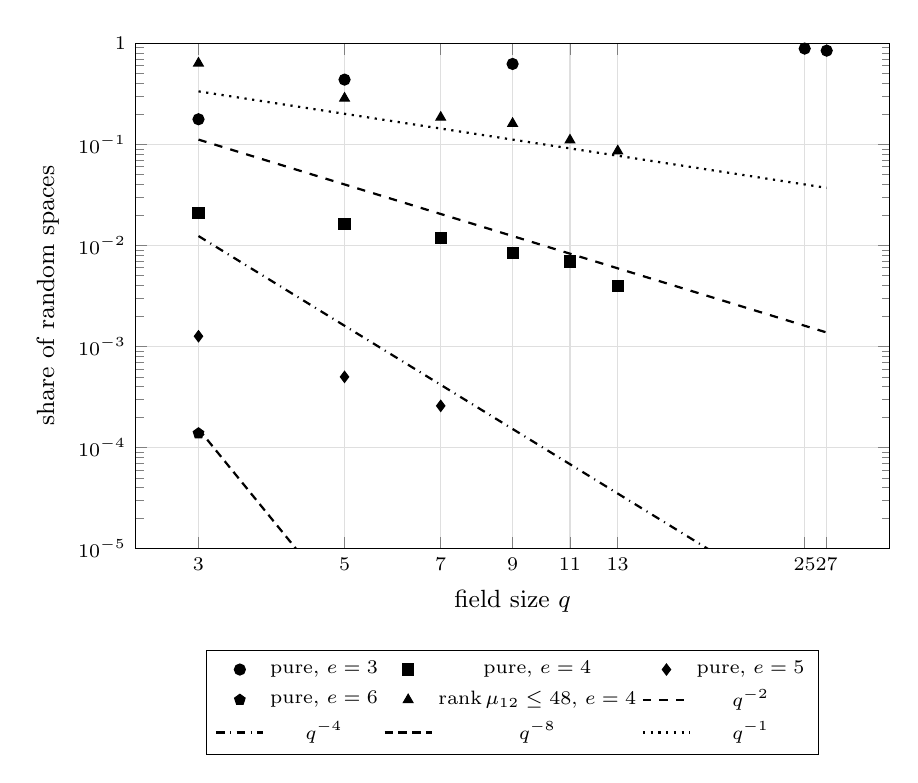
\begin{tikzpicture}
\begin{axis}[xmode=log, ymode=log, width=0.92\textwidth, height=8cm, xlabel={field size $q$}, ylabel={share of random spaces}, ymin=0.00001, ymax=1, xtick={3,5,7,9,11,13,25,27}, xticklabels={3,5,7,9,11,13,25,27}, minor xtick={}, ytick={0.00001,0.0001,0.001,0.01,0.1,1}, yticklabels={$10^{-5}$,$10^{-4}$,$10^{-3}$,$10^{-2}$,$10^{-1}$,$1$}, minor ytick={}, tick label style={font=\scriptsize}, label style={font=\small}, grid=major, grid style={gray!25}, legend style={font=\scriptsize, at={(0.5,-0.2)}, anchor=north}, legend columns=3]
\addplot[only marks, mark=*, mark size=2pt] coordinates {(3,0.176551) (5,0.435500) (9,0.622500) (25,0.883500) (27,0.843000)};
\addlegendentry{pure, $e=3$}
\addplot[only marks, mark=square*, mark size=2pt] coordinates {(3,0.021000) (5,0.016350) (7,0.011800) (9,0.008400) (11,0.006900) (13,0.003950)};
\addlegendentry{pure, $e=4$}
\addplot[only marks, mark=diamond*, mark size=2pt] coordinates {(3,0.001260) (5,0.000499) (7,0.000258)};
\addlegendentry{pure, $e=5$}
\addplot[only marks, mark=pentagon*, mark size=2pt] coordinates {(3,0.000138)};
\addlegendentry{pure, $e=6$}
\addplot[only marks, mark=triangle*, mark size=2pt] coordinates {(3,0.632800) (5,0.284600) (7,0.184250) (9,0.160200) (11,0.109650) (13,0.085700)};
\addlegendentry{rank$\,\mu_{12}\le48$, $e=4$}
\addplot[dashed, thick] coordinates {(3,0.111111111) (27,0.001371742112483)};
\addlegendentry{$q^{-2}$}
\addplot[dash dot, thick] coordinates {(3,0.012345679) (27,0.000001881676423)};
\addlegendentry{$q^{-4}$}
\addplot[densely dashed, thick] coordinates {(3,0.000152416) (27,0.000000000003541)};
\addlegendentry{$q^{-8}$}
\addplot[dotted, thick] coordinates {(3,0.33333) (27,0.037037)};
\addlegendentry{$q^{-1}$}
\end{axis}
\end{tikzpicture}

\caption{Share of random spaces of forms over $\F_q$ that are pure ($e=3$ circles, $e=4$ squares, $e=5$ diamonds, $e=6$ pentagons; the points at $q=5,7$ for $e=5$ and $q=3$ for $e=6$ are shares among the spaces done before the early stop) and, at $e=4$, that satisfy $\operatorname{rank}\mu_{12}\le48$ (triangles), against $q$ on logarithmic axes; the dashed, dash-dotted and densely dashed lines are the heuristic values $q^{-2}$, $q^{-4}$ and $q^{-8}$ for $e=4,5,6$ and the dotted line is $q^{-1}$. The rank condition follows the order $1/q$ and not $q^{-2}$, the pure share at $e=4$ lies below it, and the pure shares at $e=5,6$ lie near $q^{-4}$ and $q^{-8}$.}
\label{fig:sixshare}
\end{figure}

Figure~\ref{fig:sixshare} reads as follows. The triangles lie near the dotted line $1/q$, not on the dashed line $q^{-2}$, which is the refuted prediction; the squares lie below the triangles, since the pure spaces form a subset of the spaces with the rank condition (the common-factor spaces are among the triangles and never among the squares); the circles at $e=3$ rise with $q$, not monotonically (the share over $\F_{27}$ is below that over $\F_{25}$, two fields of different characteristic), as expected for a set that is open and dense in $G_3$ outside characteristic $2$. The figure does not show the $e=5$ share ($0.13$ percent over $\F_3$) and does not say how the shares behave beyond $q=27$.

\begin{table}[htbp]
\centering\footnotesize
\begin{tabular}{@{}rr>{\raggedright\arraybackslash}p{9.6cm}r@{}}
\toprule
$e$ & field & forms of degree $e$ & length\\
\midrule
3 & $\F_{3}$ & $f=xz + y^{3}$\newline $g=x^{3} + xz + xy^{2}$ & 27\\
3 & $\F_{5}$ & $f=-2x^{3} + x^{2}y - xy^{2} - yz - y^{3}$\newline $g=x^{3} - 2xz - 2xy^{2} - 2yz$ & 27\\
4 & $\F_{3}$ & $f=x^{4} + x^{3}y + x^{2}y^{2} - xyz + z^{2} - y^{2}z$\newline $g=x^{4} - x^{2}z - x^{2}y^{2} - xyz + z^{2} - y^{2}z - y^{4}$ & 64\\
4 & $\F_{5}$ & $f=2x^{4} - x^{3}y - 2x^{2}z - 2x^{2}y^{2} - 2xyz - xy^{3} + 2z^{2} + 2y^{2}z - y^{4}$\newline $g=-2x^{3}y - xyz + z^{2} + 2y^{2}z + 2y^{4}$ & 64\\
4 & $\F_{7}$ & $f=x^{4} + 3x^{2}z - 2x^{2}y^{2} - 2xyz - xy^{3} + 2y^{2}z + 2y^{4}$\newline $g=2x^{4} - 3x^{3}y + 2x^{2}z + 3x^{2}y^{2} - xyz - xy^{3} - 2y^{2}z$ & 64\\
5 & $\F_{3}$ & $f=-x^{3}y^{2} - x^{2}yz - x^{2}y^{3} + xz^{2} + xy^{2}z + y^{5}$\newline $g=x^{5} + x^{4}y - x^{2}yz - xz^{2} + xy^{4} + y^{3}z + y^{5}$ & 125\\
5 & $\F_{5}$ & $f=-2x^{4}y + x^{3}z + x^{3}y^{2} + 2x^{2}yz + 2x^{2}y^{3} - 2xy^{2}z - xy^{4} + yz^{2} + 2y^{3}z + 2y^{5}$\newline $g=x^{5} + x^{4}y + 2x^{3}z + x^{3}y^{2} - x^{2}y^{3} - 2xy^{2}z + xy^{4} - 2yz^{2} + y^{3}z + y^{5}$ & 125\\
5 & $\F_{7}$ & $f=3x^{5} - 2x^{3}z + x^{3}y^{2} - x^{2}yz - x^{2}y^{3} - 3xz^{2} + xy^{2}z - xy^{4} - yz^{2} - 2y^{3}z - 3y^{5}$\newline $g=-3x^{5} + x^{4}y - x^{3}z + 2x^{3}y^{2} + x^{2}yz - 2x^{2}y^{3} + 3xz^{2} - 2xy^{2}z - 3xy^{4} - 2yz^{2} - y^{3}z + y^{5}$ & 125\\
6 & $\F_{3}$ & $f=-x^{6} - x^{4}z + x^{4}y^{2} + x^{2}z^{2} - x^{2}y^{4} - xyz^{2} + xy^{3}z - xy^{5} + z^{3} + y^{4}z + y^{6}$\newline $g=-x^{3}yz + x^{3}y^{3} - x^{2}y^{2}z + x^{2}y^{4} - xyz^{2} - xy^{3}z - xy^{5} - z^{3} - y^{6}$ & 216\\
\bottomrule
\end{tabular}

\caption{One pure pair of forms $f,g\in U_e$ for each prime field of Proposition~\ref{prop:odd}, printed in the monomials $x^iy^jz^k$ with coefficients of least absolute value; each is taken from the stored basis of the space, its Hilbert function is recomputed in the script and equals $h_e$, and its Betti table is $(1,2,2,1)$ on $(0,e,3e,4e)$ in both instruments.}
\label{tab:sixpairs}
\end{table}

Table~\ref{tab:sixpairs} prints the pairs of Proposition~\ref{prop:odd}: the lengths are $\nsixPairLengthThree$, $\nsixPairLengthFour$, $\nsixPairLengthFive$ and $\nsixPairLengthSix$ ($e^3$). Singular gives the pure table on all \nsixSingularSample{} pure spaces sampled for the second instrument (the first $50$ of the exhaustive family and the first $20$ of every other family; the same for the first $20$ pure spaces of each of the three families of the later computation, $\neightSingularSample$ pure spaces in all).

\emph{The Hilbert function does not certify purity.} Among the spaces with the pure Hilbert function, many have another Betti table (Table~\ref{tab:sixcancel}): \nsixAOneThreeNonpure{} of \nsixAOneThreePureHF{} over $\F_3$ at $e=3$, \nsixBOneThreeNonpure{} of \nsixBOneThreePureHF{} over $\F_3$ at $e=4$, \neightAFiveNonpure{} of \neightAFivePureHF{} over $\F_5$ and \neightBSevenNonpure{} of \neightBSevenPureHF{} over $\F_7$ at $e=5$, and \neightCThreeNonpure{} of \neightCThreePureHF{} over $\F_3$ at $e=6$. At $e=3$ over $\F_3$ the three tables that occur differ from the pure one by a cancelling pair $\beta_{2,j}=\beta_{3,j}=1$ in degree $j=10$, in degree $j=11$, or in both; the Euler series is the same, so the Hilbert function is the same, and only the Tor computation separates them. Every count of pure spaces above is a count of computed Betti tables.

\begin{table}[htbp]
\centering\footnotesize
\begin{tabular}{@{}rr>{\raggedright\arraybackslash}p{2.2cm}r>{\raggedright\arraybackslash}p{1.8cm}>{\raggedright\arraybackslash}p{1.8cm}>{\raggedright\arraybackslash}p{2.2cm}@{}}
\toprule
$e$ & field & pure Hilbert function & pure & another table & distinct tables & share of another table\\
\midrule
3 & $\F_{3}$ & 3{,}192 & 1{,}944 & 1{,}248 & 3 & 39.1\%\\
3 & $\F_{5}$ & 1{,}340 & 871 & 469 & 3 & 35.0\%\\
3 & $\F_{9}$ & 1{,}530 & 1{,}245 & 285 & 3 & 18.6\%\\
3 & $\F_{25}$ & 1{,}906 & 1{,}767 & 139 & 3 & 7.3\%\\
3 & $\F_{27}$ & 1{,}840 & 1{,}686 & 154 & 3 & 8.4\%\\
4 & $\F_{3}$ & 917 & 420 & 497 & 7 & 54.2\%\\
4 & $\F_{5}$ & 605 & 327 & 278 & 7 & 46.0\%\\
4 & $\F_{7}$ & 356 & 236 & 120 & 6 & 33.7\%\\
4 & $\F_{9}$ & 221 & 168 & 53 & 7 & 24.0\%\\
4 & $\F_{11}$ & 173 & 138 & 35 & 5 & 20.2\%\\
4 & $\F_{13}$ & 98 & 79 & 19 & 6 & 19.4\%\\
5 & $\F_{3}$ & 191 & 63 & 128 & 13 & 67.0\%\\
5 & $\F_{5}$ & 120 & 43 & 77 & 11 & 64.2\%\\
5 & $\F_{7}$ & 70 & 42 & 28 & 9 & 40.0\%\\
6 & $\F_{3}$ & 63 & 40 & 23 & 9 & 36.5\%\\
\bottomrule
\end{tabular}

\caption{Spaces with the pure Hilbert function $h_e$ and a Betti table other than $(1,2,2,1)$: for each family and field the number with the pure Hilbert function, with the pure table, with another table (a table with a cancelling pair of Betti numbers), the number of distinct such tables and their share among the spaces with the pure Hilbert function.}
\label{tab:sixcancel}
\end{table}

\emph{The control fields.} Over $\F_{11}$ and $\F_{13}$, where $M_4$ is pure, none of the \nsixControlTotal{} pure spaces found at random contains the fourth power of a linear form over the field or over its quadratic extension, so all of them lie outside the orbit of $W_0$: the modules $U/U(l_1^e,l_2^e)$ are not the only pure cyclic modules on the ray, as the dimension bound of Theorem~\ref{thm:family} leads one to expect [MV].

\subsection{The family of pure pairs through \texorpdfstring{$\langle x^e,y^e\rangle$}{the power pair}}
\label{sec:resfamily}

Table~\ref{tab:seventangent} gives the tangent space of $D_e$ at $W_0$ (Section~\ref{sec:tangentmethods}) for $e=4,\dots,7$: the matrix $A$ has size $50\times49$, $72\times72$, $98\times100$, $128\times132$ and rank exactly $r=\nsevenRankFour$, $\nsevenRankFive$, $\nsevenRankSix$, $\nsevenRankSeven$ over $\Q$, with a left kernel of dimension $2$ and a cokernel of dimension $h_e(3e)=\nsevenCokerFour,\nsevenCokerFive,\nsevenCokerSix,\nsevenCokerSeven$. The chart has $\nsevenCoordsFour$, $\nsevenCoordsFive$, $\nsevenCoordsSix$ and $\nsevenCoordsSeven$ coordinates and $T$ has rank $2h_e(3e)$ in each case, so it is onto and the tangent dimension is $\nsevenTangentFour$, $\nsevenTangentFive$, $\nsevenTangentSix$, $\nsevenTangentSeven$, that is $4e-4$ (Proposition~\ref{prop:exact}). The two orbit directions lie in the kernel of $T$ [MV]. Over $\F_{13}$, $\F_{17}$ and $\F_{32003}$ the dimension is also $4e-4$ at $e=4,5$; at $e=6$ it is $22$ over $\F_{13}$ and $20$ over $\F_{17}$ and $\F_{32003}$; at $e=7$ it is $26$ over $\F_{17}$ and $24$ over $\F_{32003}$. The table does not show the tangent space at $e=7$ over $\F_{13}$ ($13<2e$, not computed), or any point other than $W_0$.

\begin{table}[htbp]
\centering\footnotesize
\begin{tabular}{@{}rlrrrrrrrrr@{}}
\toprule
$e$ & $A$ & $r$ & $h_e(3e)$ & chart & rank $T$ & $\Q$ & $4e-4$ & $\F_{13}$ & $\F_{17}$ & $\F_{32003}$\\
\midrule
4 & 50$\times$49 & 48 & 1 & 14 & 2 & 12 & 12 & 12 & 12 & 12\\
5 & 72$\times$72 & 70 & 2 & 20 & 4 & 16 & 16 & 16 & 16 & 16\\
6 & 98$\times$100 & 96 & 4 & 28 & 8 & 20 & 20 & 22 & 20 & 20\\
7 & 128$\times$132 & 126 & 6 & 36 & 12 & 24 & 24 & -- & 26 & 24\\
\bottomrule
\end{tabular}

\caption{The tangent space of $D_e$ at $W_0=\langle x^e,y^e\rangle$: the size of $A=\mu_{3e}(W_0)$, its rank $r$, the dimension $h_e(3e)$ of its cokernel, the number of chart coordinates $2(u(e)-2)$, the rank of $T$, the tangent dimension over $\Q$, the bound $4e-4$, and the tangent dimension over $\F_{13}$, $\F_{17}$ and $\F_{32003}$ (a dash where it was not computed).}
\label{tab:seventangent}
\end{table}

Table~\ref{tab:sevenpairs} lists explicit pairs over the rationals. $P_1,\dots,P_4$ (at $e=4$) and $P_5$ (at $e=5$) have $\operatorname{rank}\mu_{3e}=r$ and the pure table in both instruments, and $\dim(S_e+W)$ exceeds $\dim S_e=e+1$, so each lies outside the orbit of $W_0$ over every extension of $\Q$ and is no module $U/U(l_1^e,l_2^e)$ [MV]. The ranks and the orbit dimensions of the table are recomputed in the script. The controls behave as expected: $W_0$ is pure and inside the orbit; $C_1$ has rank $49$ and a table with extra Betti numbers; $C_2$ has rank $46$, below $r$, and infinite length (nonzero in every degree to $24$).

\begin{table}[htbp]
\centering\footnotesize
\begin{tabular}{@{}lr>{\raggedright\arraybackslash}p{4.9cm}>{\raggedright\arraybackslash}p{1.9cm}>{\raggedright\arraybackslash}p{2.8cm}>{\raggedright\arraybackslash}p{2.2cm}@{}}
\toprule
space & $e$ & forms over $\Q$ & rank $\mu_{3e}$ / $r$ & Betti table & $\dim(S_e{+}W)$ / $\dim S_e$\\
\midrule
$W_0$ & 4 & $f=x^{4}$\newline $g=y^{4}$ & 48 / 48 & $(1,2,2,1)$ on $(0,4,12,16)$ & 5 / 5\\
$W_0$ & 5 & $f=x^{5}$\newline $g=y^{5}$ & 70 / 70 & $(1,2,2,1)$ on $(0,5,15,20)$ & 6 / 6\\
$P_1$ & 4 & $f=x^{4} + xy^{3}$\newline $g=y^{4}$ & 48 / 48 & $(1,2,2,1)$ on $(0,4,12,16)$ & 6 / 5\\
$P_2$ & 4 & $f=x^{4} + 31x^{2}y^{2} - 8xyz$\newline $g=y^{4}$ & 48 / 48 & $(1,2,2,1)$ on $(0,4,12,16)$ & 6 / 5\\
$P_3$ & 4 & $f=x^{4} + 59x^{2}y^{2} - 4z^{2}$\newline $g=y^{4}$ & 48 / 48 & $(1,2,2,1)$ on $(0,4,12,16)$ & 6 / 5\\
$P_4$ & 4 & $f=x^{4} + 2xy^{3} - 3y^{2}z$\newline $g=5x^{3}y + 7x^{2}z + y^{4}$ & 48 / 48 & $(1,2,2,1)$ on $(0,4,12,16)$ & 6 / 5\\
$P_5$ & 5 & $f=x^{5} + 2xy^{4} - 3y^{3}z$\newline $g=5x^{4}y + 7x^{3}z + y^{5}$ & 70 / 70 & $(1,2,2,1)$ on $(0,5,15,20)$ & 8 / 6\\
$C_1$ & 4 & $f=x^{4} + x^{2}y^{2}$\newline $g=y^{4}$ & 49 / 48 & $b_{2,12}=1$, $b_{2,13}=2$, $b_{3,15}=2$ & 6 / 5\\
$C_2$ & 4 & $f=x^{4} + xy^{3}$\newline $g=x^{3}y + y^{4}$ & 46 / 48 & infinite length & 7 / 5\\
\bottomrule
\end{tabular}

\caption{Explicit spaces over $\Q$ at $e=4,5$: the forms, the rank of $\mu_{3e}$ against $r$, the Betti table, and $\dim(S_e+W)$ against $\dim S_e=e+1$ (equal for a space inside the orbit); $P_1,\dots,P_5$ are pure and outside the orbit, $W_0$ is pure and inside, $C_1$ and $C_2$ are controls that are not pure.}
\label{tab:sevenpairs}
\end{table}

Table~\ref{tab:sevenfam} reports three finite tests. The linear family $L_e(a,b,c,d)$ of~\eqref{eq:Le} has $\operatorname{rank}\mu_{3e}\le r$ on all $625$ members with parameters in $\{-2,\dots,2\}$ for $e=4$ and for $e=5$, over $\Q$; the rank equals $r$ on \nsevenLQQAtFour{} and \nsevenLQQAtFive{} of them and is lower on the others (down to \nsevenLQQMinFour{} and \nsevenLQQMinFive{}). Over $\F_{32003}$, \nsevenLGFPureFour{} of $200$ random members at $e=4$ and \nsevenLGFPureFive{} of $200$ at $e=5$ are pure and outside the orbit. These are tests of Proposition~\ref{prop:linear}, which proves the inclusion of $L_e$ in $D_e$ for every parameter and every $e\ge4$ in characteristic $0$ or at least $2e$ [D]; the machine values confirm it on the members listed, over $\Q$ and over $\F_{32003}$ [MV]. The plane section $\langle x^4+\alpha x^2y^2+\beta xyz+\gamma z^2,\ y^4\rangle$ over the grid $\{-4,\dots,4\}^3$ ($\nsevenGridSpaces$ spaces) has $\operatorname{rank}\mu_{12}\le48$ at no point off the plane $8\alpha+31\beta+118\gamma=0$ (\nsevenGridOff{} points with rank $49$); the grid meets the plane only at the origin, so the converse direction rests on the origin and on the six pure spaces $t\,(31,-8,0)$ and $t\,(59,0,-4)$, $t=1,2,3$, which are pure over $\Q$ [MV on the tested points; the equation of the plane is not proved here [U]]. Finally, spaces whose two forms have a common factor modulo $z$ satisfy $\operatorname{rank}\mu_{3e}\le r$ on all $\nsevenCommon$ random spaces tested over $\F_{32003}$ at each of $e=4,5,6$ (common factors of degree $1,2,4=h_e(3e)$), and at $e=4$ all have infinite length: the component of $D_e$ with no pure point of Remark~\ref{rem:common} [MV].

\begin{table}[htbp]
\centering\footnotesize
\begin{tabular}{@{}lrlrrrr@{}}
\toprule
family & $e$ & field and sampling & spaces & rank $\le r$ & rank $=r$ & pure, outside orbit\\
\midrule
$L_4$ & 4 & $\Q$, parameters in $\{-2,\dots,2\}$ & 625 & 625 & 569 & --\\
$L_4$ & 4 & $\F_{32003}$, random & 200 & 200 & 200 & 200\\
$L_5$ & 5 & $\Q$, parameters in $\{-2,\dots,2\}$ & 625 & 625 & 571 & --\\
$L_5$ & 5 & $\F_{32003}$, random & 200 & 200 & 200 & 200\\
section $\Pi$ & 4 & $\Q$, grid $\{-4,\dots,4\}^3$ & 729 & 1 & 1 & --\\
common factor of degree 1 & 4 & $\F_{32003}$, random & 20 & 20 & 20 & --\\
common factor of degree 2 & 5 & $\F_{32003}$, random & 20 & 20 & 20 & --\\
common factor of degree 4 & 6 & $\F_{32003}$, random & 20 & 20 & 20 & --\\
\bottomrule
\end{tabular}

\caption{Finite tests at the power pair: the linear family $L_e$, the plane section $\Pi$ and the common-factor locus; the number of spaces tested, with $\operatorname{rank}\mu_{3e}\le r$, with $\operatorname{rank}\mu_{3e}=r$, and pure and outside the orbit (a dash where purity was not tested); all members satisfy the rank bound, and the section has one space with rank at most $r$ among $729$, the origin.}
\label{tab:sevenfam}
\end{table}

\subsection{The linear family below characteristic \texorpdfstring{$2e$}{2e}}
\label{sec:reslf}

Proposition~\ref{prop:linear} proves the inclusion $L_e\subset D_e$ and the purity of the general member in characteristic $0$ or at least $2e$. Below $2e$ the proof does not apply (Remark after Proposition~\ref{prop:linear}), and Table~\ref{tab:lfam} reports the enumeration of Section~\ref{sec:lfmethods}: for each pair $(e,p)$ with $4\le e\le7$ the number of members over $\F_p$ ($p^4$), the number of rank exactly $r$, the number above $r$, the number of members of rank $r$ examined, those with the pure Hilbert function and those with the pure Betti table, and for the pairs where the enumeration over $\F_p$ finds no pure member the sample of $20{,}000$ members over $\F_{p^2}$.

\begin{table}[htbp]
\centering\footnotesize
\begin{tabular}{@{}rrrrrrrrrl@{}}
\toprule
$e$ & $p$ & members & rank $r$ & rank $>r$ & examined & pure $h_e$ & pure & $\F_{p^2}$: pure of rank $r$ & reading\\
\midrule
4 & 3 & 81 & 0 & 0 & 0 & 0 & 0 & 0 of 0 & no pure member\\
4 & 5 & 625 & 268 & 0 & 240 & 159 & 95 & -- & pure members\\
4 & 7 & 2{,}401 & 1{,}626 & 0 & 208 & 130 & 98 & -- & pure members\\
4 & 11 & 14{,}641 & 12{,}211 & 0 & 160 & 155 & 150 & -- & control\\
4 & 13 & 28{,}561 & 24{,}997 & 0 & 160 & 160 & 160 & -- & control\\
5 & 3 & 81 & 0 & 0 & 0 & 0 & 0 & 0 of 0 & no pure member\\
5 & 5 & 625 & 212 & 0 & 212 & 0 & 0 & 0 of 15{,}798 & no pure member\\
5 & 7 & 2{,}401 & 1{,}158 & 0 & 192 & 138 & 110 & -- & pure members\\
5 & 11 & 14{,}641 & 9{,}941 & 0 & 160 & 156 & 150 & -- & control\\
5 & 13 & 28{,}561 & 22{,}945 & 0 & 160 & 160 & 160 & -- & control\\
6 & 3 & 81 & 0 & 0 & 0 & 0 & 0 & 0 of 0 & no pure member\\
6 & 5 & 625 & 0 & 0 & 0 & 0 & 0 & 0 of 0 & no pure member\\
6 & 7 & 2{,}401 & 918 & 0 & 918 & 0 & 0 & 0 of 17{,}059 & no pure member\\
6 & 11 & 14{,}641 & 10{,}670 & 0 & 208 & 121 & 99 & -- & pure members\\
6 & 13 & 28{,}561 & 20{,}545 & 0 & 160 & 160 & 160 & -- & control\\
7 & 3 & 81 & 0 & 0 & 0 & 0 & 0 & 0 of 0 & no pure member\\
7 & 5 & 625 & 0 & 0 & 0 & 0 & 0 & 0 of 0 & no pure member\\
7 & 7 & 2{,}401 & 0 & 0 & 0 & 0 & 0 & 0 of 0 & no pure member\\
7 & 11 & 14{,}641 & 8{,}050 & 0 & 200 & 134 & 111 & -- & pure members\\
7 & 13 & 28{,}561 & 21{,}012 & 0 & 192 & 122 & 111 & -- & pure members\\
\bottomrule
\end{tabular}

\caption{The linear family $L_e(a,b,c,d)$ over $\F_p$ for $4\le e\le7$ and the odd primes $p\le13$ (twenty pairs: $p<2e$ for fifteen of them, the other five are control pairs with $p\ge2e$): the number of members ($p^4$), of rank $\mu_{3e}$ exactly $r=2u(2e)-2$, above $r$, the number of members of rank $r$ examined (all of them, or the first ones in the lexicographic order of the parameters when the second stage stopped early), those with the pure Hilbert function, those with the pure Betti table, and, for the nine pairs below $2e$ without a pure member over $\F_p$, the pure members among the members of rank $r$ in a sample of $20{,}000$ over $\F_{p^2}$.}
\label{tab:lfam}
\end{table}

\emph{The inclusion in the rank locus.} In all fifteen pairs below $2e$ no member of the family has $\operatorname{rank}\mu_{3e}>r$: none of the \nlfFamilyMembersBelow{} members over $\F_p$, and none of the \nlfYMembers{} members sampled over $\F_{p^2}$ in \nlfYPairs{} pairs. The rank distribution is wide (Table~\ref{tab:lfam} gives the members of rank exactly $r$), and the inclusion $L_e\subset D_e$ of Proposition~\ref{prop:linear} therefore holds on every member computed in characteristics below $2e$, although the proof does not reach them [MV]. This is an observation on finite fields; it is not proved there.

\emph{Pure members for $e<p<2e$.} In six of the seven pairs with $e<p<2e$ the family holds pure members over $\F_p$: $(4,5)$ with \nlfFourFivePure{} pure among \nlfFourFiveExamined{} members of rank $r$ examined, $(4,7)$ with \nlfFourSevenPure{} among \nlfFourSevenExamined{}, $(5,7)$ with \nlfFiveSevenPure{} among \nlfFiveSevenExamined{}, $(6,11)$ with \nlfSixElevenPure{} among \nlfSixElevenExamined{}, $(7,11)$ with \nlfSevenElevenPure{} among \nlfSevenElevenExamined{} and $(7,13)$ with \nlfSevenThirteenPure{} among \nlfSevenThirteenExamined{} (each pair stopped early; the counts are among the members examined). Table~\ref{tab:lfampairs} prints the first pure member of each pair; the script recomputes its Hilbert function (which equals $h_e$) and the rank of $\mu_{3e}$ (which equals $r$) in its own arithmetic, and Singular gives the pure table on the first five pure members of each of these pairs and of the control pairs ($\nlfSingularSample$ members in all). So the point $(1,2,2,1)$ of $(0,6,18,24)$ is realized in characteristic $11$, and that of $(0,7,21,28)$ in characteristics $11$ and $13$ [MV]. At $(6,7)$ the family has no pure member: all \nlfSixSevenRankR{} members of rank $r$ over $\F_7$ were examined, and so were all \nlfYSixSevenRankR{} of rank $r$ among the $20{,}000$ sampled over $\F_{49}$; none has the pure Hilbert function [MV]. This is a statement about this family over those two fields, not about other pairs of forms or larger extensions.

\begin{table}[htbp]
\centering\footnotesize
\begin{tabular}{@{}lc>{\raggedright\arraybackslash}p{5.4cm}rl@{}}
\toprule
$(e,p)$ & $(a,b,c,d)$ & forms over $\F_p$ & length & Betti table (both instruments)\\
\midrule
$(4,5)$ & $(0,1,0,3)$ & $f=x^{4} + y^{2}z$\newline $g=-2x^{2}z + y^{4}$ & 64 & $(1,2,2,1)$ on $(0,4,12,16)$\\
$(4,7)$ & $(0,1,0,1)$ & $f=x^{4} + y^{2}z$\newline $g=x^{2}z + y^{4}$ & 64 & $(1,2,2,1)$ on $(0,4,12,16)$\\
$(5,7)$ & $(0,1,0,1)$ & $f=x^{5} + y^{3}z$\newline $g=x^{3}z + y^{5}$ & 125 & $(1,2,2,1)$ on $(0,5,15,20)$\\
$(6,11)$ & $(0,1,0,3)$ & $f=x^{6} + y^{4}z$\newline $g=3x^{4}z + y^{6}$ & 216 & $(1,2,2,1)$ on $(0,6,18,24)$\\
$(7,11)$ & $(0,1,0,3)$ & $f=x^{7} + y^{5}z$\newline $g=3x^{5}z + y^{7}$ & 343 & $(1,2,2,1)$ on $(0,7,21,28)$\\
$(7,13)$ & $(0,1,0,1)$ & $f=x^{7} + y^{5}z$\newline $g=x^{5}z + y^{7}$ & 343 & $(1,2,2,1)$ on $(0,7,21,28)$\\
\bottomrule
\end{tabular}

\caption{The first pure member of the linear family for each pair $(e,p)$ with $e<p<2e$ where the family holds one: the parameters $(a,b,c,d)$ of $L_e$, the forms over $\F_p$ (coefficients of least absolute value), the length of $U/(Uf+Ug)$ and its Betti table, equal to $(1,2,2,1)$ on $(0,e,3e,4e)$ in the exact library and in Singular; the script recomputes the Hilbert function and the rank of $\mu_{3e}$ of each printed pair.}
\label{tab:lfampairs}
\end{table}

\emph{Characteristic at most $e$.} In the eight pairs $(4,3)$, $(5,3)$, $(5,5)$, $(6,3)$, $(6,5)$, $(7,3)$, $(7,5)$ and $(7,7)$ the family holds no pure member. In seven of them no member has rank exactly $r$, over $\F_p$ (every member) and over $\F_{p^2}$ (the $20{,}000$ sampled): every member has rank below $r$. At $(5,5)$, \nlfFiveFiveRankR{} of the $625$ members over $\F_5$ and \nlfYFiveFiveRankR{} of $20{,}000$ over $\F_{25}$ have rank $r$, and none has the pure Hilbert function [MV]. The control pairs with $p\ge2e$ behave as Proposition~\ref{prop:linear} says: every member has rank at most $r$, and at least half of the members of rank $r$ examined are pure ($\nlfFourElevenPure$ of $\nlfFourElevenExamined$ at $(4,11)$, $\nlfFourThirteenPure$ of $\nlfFourThirteenExamined$ at $(4,13)$, $\nlfFiveElevenPure$ of $\nlfFiveElevenExamined$ at $(5,11)$, $\nlfFiveThirteenPure$ of $\nlfFiveThirteenExamined$ at $(5,13)$ and $\nlfSixThirteenPure$ of $\nlfSixThirteenExamined$ at $(6,13)$) [MV]. Among the members with the pure Hilbert function some have another Betti table (for example $\nlfFourFiveNonPure$ of the $\nlfFourFiveTables$ tables computed at $(4,5)$ and $\nlfSixElevenNonPure$ of the $\nlfSixElevenTables$ at $(6,11)$), as in Section~\ref{sec:resodd}: the count of pure members is a count of computed Betti tables. \emph{The rule.} In the pairs with $e<p<2e$ computed in this paper (the pairs of this subsection, those of Sections~\ref{sec:resstrata}, \ref{sec:resmid} and~\ref{sec:reslinrule}) the stratum of the linear family holds pure members exactly when $2e-p\le3$. The half ``none when $2e-p\ge5$'' is Corollary~\ref{cor:linstratum}, for every $e\ge4$; the half ``pure members when $2e-p\in\{1,3\}$'' is computed (Table~\ref{tab:rule}) and is not proved.

\subsection{Central pairs}
\label{sec:rescen}

Table~\ref{tab:central} lists the \ncenCases{} cases of Theorem~\ref{thm:central} that were computed: the family $T$ with $A=x^e$, $B=y^e$ and linear forms $(l_1,l_2)$ for $(e,p)=(3,3)$, $(5,5)$, $(7,7)$, $(9,3)$, $(11,11)$, $(13,13)$, $(15,3)$ and $(15,5)$, and the family $G$ with central forms that are not monomials at $(9,3)$, $(5,5)$ and $(15,5)$. In every case the identities hold ($A$ and $B$ commute with $x$ and $y$, $gf-fg=\lambda z^e$, the two syzygies $s_1$, $s_2$ and the relation $gs_1+fs_2=0$), the Hilbert function equals $h_e$, the length is $e^3$ (from $27$ to \ncenMaxLength{}), and both instruments give the Betti table $(1,2,2,1)$ on $(0,e,3e,4e)$ [MV]. The script recomputes the commutator of every case in its own arithmetic and the Hilbert function and the length of every case with $e\le13$. The computations took \ncenSeconds{} seconds in all.

\begin{table}[htbp]
\centering\footnotesize
\begin{tabular}{@{}ll>{\raggedright\arraybackslash}p{6.2cm}rrl@{}}
\toprule
case & $(e,p)$ & forms over $\F_p$ & $\lambda$ & length & pure in both instruments\\
\midrule
T1 & $(3,3)$ & $f=x^{3} + yz$\newline $g=xz + y^{3}$ & 1 & 27 & yes\\
T2 & $(3,3)$ & $f=x^{3} + xz + yz$\newline $g=xz - yz + y^{3}$ & 2 & 27 & yes\\
T3 & $(5,5)$ & $f=x^{5} + yz^{2}$\newline $g=xz^{2} + y^{5}$ & 1 & 125 & yes\\
T4 & $(5,5)$ & $f=x^{5} + 2yz^{2}$\newline $g=-2xz^{2} + y^{5}$ & 1 & 125 & yes\\
T5 & $(7,7)$ & $f=x^{7} + yz^{3}$\newline $g=xz^{3} + y^{7}$ & 1 & 343 & yes\\
T6 & $(7,7)$ & $f=x^{7} + 3yz^{3}$\newline $g=-2xz^{3} + y^{7}$ & 1 & 343 & yes\\
T7 & $(7,7)$ & $f=x^{7} + xz^{3}$\newline $g=yz^{3} + y^{7}$ & 6 & 343 & yes\\
T8 & $(9,3)$ & $f=x^{9} + yz^{4}$\newline $g=xz^{4} + y^{9}$ & 1 & 729 & yes\\
T9 & $(9,3)$ & $f=x^{9} + xz^{4} + yz^{4}$\newline $g=yz^{4} + y^{9}$ & 2 & 729 & yes\\
T10 & $(11,11)$ & $f=x^{11} + yz^{5}$\newline $g=xz^{5} + y^{11}$ & 1 & 1331 & yes\\
T11 & $(13,13)$ & $f=x^{13} + yz^{6}$\newline $g=xz^{6} + y^{13}$ & 1 & 2197 & yes\\
T12 & $(15,3)$ & $f=x^{15} + yz^{7}$\newline $g=xz^{7} + y^{15}$ & 1 & 3375 & yes\\
T13 & $(15,5)$ & $f=x^{15} + yz^{7}$\newline $g=xz^{7} + y^{15}$ & 1 & 3375 & yes\\
G1 & $(9,3)$ & $f=x^{9} + x^{3}y^{6} + yz^{4}$\newline $g=x^{9} + x^{6}y^{3} + xz^{4} + y^{9}$ & 1 & 729 & yes\\
G2 & $(5,5)$ & $f=x^{5} + yz^{2} + 2y^{5}$\newline $g=-2x^{5} + xz^{2} + 2y^{5}$ & 1 & 125 & yes\\
G3 & $(15,5)$ & $f=x^{15} + x^{10}y^{5} + yz^{7}$\newline $g=x^{15} + 2x^{5}y^{10} + xz^{7} + y^{15}$ & 1 & 3375 & yes\\
\bottomrule
\end{tabular}

\caption{The pairs of Theorem~\ref{thm:central} that were computed: the case ($T$: $A=x^e$, $B=y^e$; $G$: central forms that are not monomials), $(e,p)$, the forms over $\F_p$, the scalar $\lambda$ with $gf-fg=\lambda z^e$, the length of $U/(Uf+Ug)$ and whether the Betti table is $(1,2,2,1)$ on $(0,e,3e,4e)$ in both instruments; the length is $e^3$ in every case.}
\label{tab:central}
\end{table}

So the point $(1,2,2,1)$ is realized by explicit pairs confirmed in two instruments on $(0,7,21,28)$ in characteristic $7$, for example by $f=x^7+yz^3$ and $g=y^7+xz^3$ (length $343$), on $(0,9,27,36)$ in characteristic $3$ (length $729$), on $(0,11,33,44)$ in characteristic $11$, on $(0,13,39,52)$ in characteristic $13$, and on $(0,15,45,60)$ in characteristics $3$ and $5$ [MV]. The cases with linear forms $(x+y,x-y)$, $(2y,3x)$, $(x,y)$ and $(x+y,y)$ and with central forms that are not monomials behave as the theorem says. The experiment checks cases; the statement for every odd $e$ and every prime $p$ dividing $e$ rests on the proof [D].

\subsection{The criterion on explicit and random pairs}
\label{sec:rescrit}

Table~\ref{tab:critpairs} lists the \ncritXCases{} explicit pairs of Corollary~\ref{cor:cases} that were computed: case B at $(4,3)$, $(6,5)$, $(8,7)$, $(10,3)$ and $(12,11)$; case C at $(6,3)$, $(10,5)$ and $(12,3)$; case D at $(7,3)$, $(11,5)$ and $(13,3)$. In each the commutator is $-Dz$ (recomputed by the script with $D$ recomputed from the data of the pair), the two syzygies and the third relation hold, the ideal $(zD,n(f),n(g))$ is zero dimensional, the Hilbert function is $h_e$, the length is $e^3$ (from \ncritMinLength{} to \ncritMaxLength{}), and both instruments give the Betti table $(1,2,2,1)$ on $(0,e,3e,4e)$ [MV]. So the point $(1,2,2,1)$ of $(0,6,18,24)$ is realized in characteristic $5$ by $f=x^6+z^3$, $g=y^6+z^3$ (length $216$), and that of $(0,7,21,28)$ in characteristic $3$ by $f=x^7+yz^3+x^3z^2$, $g=y^7+xz^3$ (length $343$); neither pair is reached by the searches of Section~\ref{sec:resodd}. The pairs of case B reach $e=8$ in characteristic $7$, $e=10$ in characteristic $3$ and $e=12$ in characteristic $11$; case C reaches $e=10$ in characteristic $5$ and $e=12$ in characteristic $3$; case D reaches $e=11$ in characteristic $5$ and $e=13$ in characteristic $3$.

\begin{table}[htbp]
\centering\footnotesize
\begin{tabular}{@{}lll>{\raggedright\arraybackslash}p{6.0cm}r@{}}
\toprule
case & $(e,p)$ & type & forms over $\F_p$ & length\\
\midrule
B1 & $(4,3)$ & B & $f=x^{4} + z^{2}$\newline $g=z^{2} + y^{4}$ & 64\\
B2 & $(6,5)$ & B & $f=x^{6} + z^{3}$\newline $g=z^{3} + y^{6}$ & 216\\
B3 & $(8,7)$ & B & $f=x^{8} + z^{4}$\newline $g=z^{4} + y^{8}$ & 512\\
B4 & $(10,3)$ & B & $f=x^{10} + z^{5}$\newline $g=z^{5} + y^{10}$ & 1000\\
B5 & $(12,11)$ & B & $f=x^{12} + z^{6}$\newline $g=z^{6} + y^{12}$ & 1728\\
C1 & $(6,3)$ & C & $f=x^{6} + z^{3} + y^{4}z$\newline $g=x^{4}z + y^{6}$ & 216\\
C2 & $(10,5)$ & C & $f=x^{10} + z^{5} + y^{6}z^{2}$\newline $g=x^{6}z^{2} + y^{10}$ & 1000\\
C3 & $(12,3)$ & C & $f=x^{12} + z^{6} + y^{4}z^{4}$\newline $g=x^{4}z^{4} + y^{12}$ & 1728\\
D1 & $(7,3)$ & D & $f=x^{7} + x^{3}z^{2} + yz^{3}$\newline $g=xz^{3} + y^{7}$ & 343\\
D2 & $(11,5)$ & D & $f=x^{11} + x^{5}z^{3} + yz^{5}$\newline $g=xz^{5} + y^{11}$ & 1331\\
D3 & $(13,3)$ & D & $f=x^{13} + x^{3}z^{5} + yz^{6}$\newline $g=xz^{6} + y^{13}$ & 2197\\
\bottomrule
\end{tabular}

\caption{The explicit pairs of Corollary~\ref{cor:cases} that were computed (cases B, C, D): the case, $(e,p)$, the type, the forms over $\F_p$ and the length of $U/(Uf+Ug)$ (equal to $e^3$); each has $gf-fg=-Dz$, a zero dimensional ideal $(zD,n(f),n(g))$, the Hilbert function $h_e$ and the Betti table $(1,2,2,1)$ on $(0,e,3e,4e)$ in both instruments.}
\label{tab:critpairs}
\end{table}

Table~\ref{tab:critrand} compares the criterion with purity on random pairs of the class. For each of the eight pairs $(e,p)$ there are $200$ pairs with uniform coefficients on the basis of $V_e$; the identity $gf-fg=-Dz$ holds on all \ncritRandomPairs{} of them, the criterion is true on \ncritRandomPure{} of them, and exactly on those the Hilbert function is $h_e$: the criterion and the pure Hilbert function agree on every pair, and all \ncritRandomBetti{} Betti tables computed (ten per case) are pure [MV]. Between \ncritShareMin{} and \ncritShareMax{} percent of the pairs of the class are pure in the eight cases. The agreement is the equivalence of (i) and (iii) of Theorem~\ref{thm:crit} tested on $1{,}600$ pairs; it does not replace the proof.

\begin{table}[htbp]
\centering\footnotesize
\begin{tabular}{@{}lrrrrrrrr@{}}
\toprule
$(e,p)$ & seed & pairs & identity holds & criterion true & pure $h_e$ & disagree & pure Betti tables & share (\%)\\
\midrule
$(4,3)$ & 20261120 & 200 & 200 & 66 & 66 & 0 & 10 of 10 & 33.0\\
$(6,3)$ & 20261121 & 200 & 200 & 79 & 79 & 0 & 10 of 10 & 39.5\\
$(6,5)$ & 20261122 & 200 & 200 & 117 & 117 & 0 & 10 of 10 & 58.5\\
$(7,3)$ & 20261123 & 200 & 200 & 44 & 44 & 0 & 10 of 10 & 22.0\\
$(7,7)$ & 20261124 & 200 & 200 & 143 & 143 & 0 & 10 of 10 & 71.5\\
$(8,7)$ & 20261125 & 200 & 200 & 134 & 134 & 0 & 10 of 10 & 67.0\\
$(9,3)$ & 20261126 & 200 & 200 & 45 & 45 & 0 & 10 of 10 & 22.5\\
$(10,3)$ & 20261127 & 200 & 200 & 73 & 73 & 0 & 10 of 10 & 36.5\\
\bottomrule
\end{tabular}

\caption{Random pairs of the class $V_e$ over $\F_p$: for each $(e,p)$ the seed, the number of pairs, the pairs on which $gf-fg=-Dz$ holds, on which the criterion of Theorem~\ref{thm:crit} is true, with the pure Hilbert function $h_e$, on which exactly one of the two holds, the Betti tables computed (the first ten pairs with the pure Hilbert function) that are pure, and the share of pure pairs in percent.}
\label{tab:critrand}
\end{table}

\subsection{Pure pairs in the weight-class strata}
\label{sec:resstrata}

The search of Section~\ref{sec:strsearch} examined \nwcStrata{} strata and \nwcMembers{} members in all (computation \EXP{010}, run in two parts with the same routine). Table~\ref{tab:wcounts} gives, for each pair and family, the number of strata, those with a member of rank $r$ and those with a pure member, the numbers of members examined, of rank $r$, with the pure Hilbert function and with the pure Betti table, and the share of the pure Hilbert function in $S(2;0,1)$ against $p^{-h_e(3e)}$; the shares and the ratios are over the members examined, and the early stop biases them. The tables of the pure members are computed by the exact library and confirmed by Singular on a sample of \nwcSingular{} pure members (the first two of each stratum that has one), with the same table on all of them [MV].

\begin{table}[htbp]
\centering\scriptsize
\begin{tabular}{@{}lrrrrrrrrrrll@{}}
\toprule
fam. & $e$ & $p$ & strata & rank $r$ & pure & examined & rank $r$ & pure $h_e$ & tables & pure & share in $S(2;0,1)$ & ratio\\
\midrule
C & 4 & 3 & 34 & 3 & 3 & 139{,}714 & 3{,}672 & 2{,}361 & 37 & 18 & 0.036 (174 of 4{,}840) & 0.11\\
C & 4 & 5 & 34 & 4 & 4 & 144{,}044 & 3{,}362 & 2{,}158 & 52 & 23 & 0.0774 (774 of 10{,}000) & 0.39\\
C & 5 & 3 & 55 & 5 & 1 & 157{,}805 & 2{,}384 & 164 & 22 & 5 & 0.0137 (164 of 12{,}000) & 0.12\\
C & 5 & 5 & 55 & 7 & 2 & 180{,}841 & 7{,}727 & 301 & 38 & 19 & 0.0174 (191 of 11{,}000) & 0.43\\
C & 5 & 7 & 55 & 12 & 5 & 204{,}575 & 12{,}568 & 1{,}142 & 76 & 42 & 0.0142 (242 of 17{,}000) & 0.70\\
C & 6 & 3 & 83 & 6 & 1 & 349{,}286 & 7{,}524 & 85 & 12 & 7 & 0.00531 (85 of 16{,}000) & 0.43\\
C & 6 & 11 & 83 & 25 & 11 & 573{,}438 & 45{,}517 & 5{,}919 & 159 & 90 & 0 (0 of 20{,}000) & 0.00\\
C & 7 & 11 & 119 & 35 & 8 & 664{,}934 & 35{,}913 & 5{,}491 & 87 & 68 & 0 (0 of 20{,}000) & 0.00\\
C & 7 & 13 & 119 & 39 & 8 & 683{,}713 & 41{,}333 & 5{,}485 & 135 & 93 & 0 (0 of 20{,}000) & 0.00\\
Q & 6 & 5 & 34 & 9 & 7 & 335{,}627 & 18{,}843 & 337 & 99 & 44 & 0.001 (20 of 20{,}000) & 0.62\\
Q & 6 & 7 & 34 & 12 & 7 & 1{,}108{,}987 & 71{,}050 & 414 & 112 & 52 & 0.000517 (30 of 58{,}000) & 1.24\\
Q & 7 & 3 & 34 & 5 & 2 & 215{,}769 & 3{,}720 & 244 & 28 & 22 & 0.000686 (15 of 21{,}870) & 0.50\\
Q & 7 & 5 & 34 & 5 & 3 & 3{,}988{,}779 & 49{,}270 & 68 & 52 & 15 & 4.27e-05 (20 of 468{,}750) & 0.67\\
Q & 7 & 7 & 34 & 4 & 4 & 26{,}574{,}117 & 51{,}025 & 183 & 43 & 21 & 6.3e-06 (9 of 1{,}428{,}000) & 0.74\\
E & 8 & 3 & 21 & 9 & 5 & 2{,}306{,}090 & 143{,}685 & 553 & 124 & 31 & 2.92e-05 (10 of 342{,}000) & 0.58\\
E & 8 & 5 & 5 & 3 & 0 & 878{,}930 & 17{,}948 & 0 & 0 & 0 & -- & --\\
E & 8 & 7 & 5 & 4 & 1 & 2{,}486{,}049 & 265{,}581 & 7 & 6 & 5 & -- & --\\
E & 8 & 11 & 1 & 1 & 0 & 17{,}689 & 6{,}010 & 0 & 0 & 0 & -- & --\\
E & 8 & 13 & 1 & 1 & 1 & 33{,}489 & 16{,}356 & 11{,}124 & 8 & 8 & -- & --\\
\bottomrule
\end{tabular}

\caption{The search in the weight-class strata: family C (controls on settled pairs), Q (the five open pairs $(6,5)$, $(6,7)$, $(7,3)$, $(7,5)$, $(7,7)$) and E ($e=8$, exploratory); for each pair the number of strata stored, with a member of rank $r$ and with a pure member, the members examined, with $\operatorname{rank}\mu_{3e}=r$, with the pure Hilbert function, the Betti tables computed and the pure ones, and the share of the pure Hilbert function in $S(2;0,1)$ (the number of such members among the members examined) with its ratio to $p^{-h_e(3e)}$.}
\label{tab:wcounts}
\end{table}

\emph{The five pairs open after the linear family.} Each of $(6,5)$, $(6,7)$, $(7,3)$, $(7,5)$, $(7,7)$ has pure pairs over $\F_p$ in admissible strata: $\nwcQSixFivePure$ pure members in \nwcQSixFiveStrataPure{} strata among \nwcQSixFiveExamined{} members at $(6,5)$, \nwcQSixSevenPure{} in \nwcQSixSevenStrataPure{} strata among \nwcQSixSevenExamined{} at $(6,7)$, \nwcQSevenThreePure{} in \nwcQSevenThreeStrataPure{} strata among \nwcQSevenThreeExamined{} at $(7,3)$, \nwcQSevenFivePure{} in \nwcQSevenFiveStrataPure{} strata among \nwcQSevenFiveExamined{} at $(7,5)$ and \nwcQSevenSevenPure{} in \nwcQSevenSevenStrataPure{} strata among \nwcQSevenSevenExamined{} at $(7,7)$; all admissible strata of each pair were run. Table~\ref{tab:wcstrata} lists the strata, and Table~\ref{tab:wcpairs} prints one pair for each of these pairs and for the pairs at $e=8$ below; the script recomputes the Hilbert function (which equals $h_e$), the length ($e^3$) and the rank of $\mu_{3e}$ of each printed pair, and checks that its forms lie in the stratum named. So the point $(1,2,2,1)$ of $(0,6,18,24)$ is realized over $\F_5$ and over $\F_7$, and that of $(0,7,21,28)$ over $\F_3$, $\F_5$ and $\F_7$ [MV, two instruments, and the pairs rebuilt by a separate parser]. With the earlier computations this gives a pure pair of degree $e$ over $\F_p$ for every odd prime $p$ below $2e$ and every $e$ from $2$ to $7$.

\begin{table}[htbp]
\centering\footnotesize
\begin{tabular}{@{}l>{\raggedright\arraybackslash}p{11.2cm}@{}}
\toprule
$(e,p)$ & strata with pure members (number of pure members)\\
\midrule
$(6,5)$ & $S(6;0,3)$ (8), $S(4;0,2)$ (8), $S(3;0,2)$ (7), $S(3;0,1)$ (6), $S(3;0,0)$ (6), $S(2;0,1)$ (4), $S(2;0,0)$ (5)\\
$(6,7)$ & $S(6;0,3)$ (7), $S(4;0,2)$ (8), $S(3;0,2)$ (8), $S(3;0,1)$ (10), $S(3;0,0)$ (9), $S(2;0,1)$ (5), $S(2;0,0)$ (5)\\
$(7,3)$ & $S(4;0,3)$ (15), $S(2;0,1)$ (7)\\
$(7,5)$ & $S(4;0,3)$ (6), $S(3;0,1)$ (5), $S(2;0,1)$ (4)\\
$(7,7)$ & $S(5;0,2)$ (6), $S(4;0,3)$ (5), $S(3;0,1)$ (5), $S(2;0,1)$ (5)\\
$(8,3)$ & $S(4;0,3)$ (4), $S(4;0,2)$ (6), $S(4;0,0)$ (11), $S(2;0,1)$ (5), $S(2;0,0)$ (5)\\
$(8,5)$ & none\\
$(8,7)$ & $S(5;0,3)$ (5)\\
$(8,11)$ & none\\
$(8,13)$ & $S(7;0,1)$ (8)\\
\bottomrule
\end{tabular}

\caption{For each pair examined by the search in the strata (the settled pairs of family C are not listed), the strata in which a pure member was found, with the number of pure members of each; at $(6,11)$ and the other settled pairs of family C the strata of the linear family hold the members of Table~\ref{tab:lfampairs}.}
\label{tab:wcstrata}
\end{table}

\begin{table}[htbp]
\centering\footnotesize
\begin{tabular}{@{}ll>{\raggedright\arraybackslash}p{6.4cm}r@{}}
\toprule
$(e,p)$ & stratum & forms over $\F_p$ & length\\
\midrule
$(6,5)$ & $S(6;0,3)$ & $f=x^{6} + y^{6}$\newline $g=x^{3}y^{3} - 2x^{2}y^{2}z - 2xyz^{2} + z^{3}$ & 216\\
$(6,7)$ & $S(6;0,3)$ & $f=x^{6} + y^{6}$\newline $g=x^{3}y^{3} + x^{2}y^{2}z + 3z^{3}$ & 216\\
$(7,3)$ & $S(4;0,3)$ & $f=x^{7} + x^{3}y^{4} + yz^{3}$\newline $g=x^{2}yz^{2} + xz^{3} + y^{7}$ & 343\\
$(7,5)$ & $S(4;0,3)$ & $f=2x^{7} + x^{3}y^{4} + x^{2}y^{3}z + 2yz^{3}$\newline $g=2x^{4}y^{3} - x^{3}y^{2}z + 2x^{2}yz^{2} - xz^{3} - 2y^{7}$ & 343\\
$(7,7)$ & $S(5;0,2)$ & $f=x^{7} + x^{2}y^{5} + 2xy^{4}z - 3y^{3}z^{2}$\newline $g=2x^{5}y^{2} + 3x^{4}yz + x^{3}z^{2} + y^{7}$ & 343\\
$(8,3)$ & $S(4;0,3)$ & $f=-x^{8} - x^{4}y^{4} - x^{3}y^{3}z + x^{2}y^{2}z^{2} + xyz^{3} - z^{4} - y^{8}$\newline $g=x^{5}y^{3} - x^{2}z^{3} + xy^{7} - y^{6}z$ & 512\\
$(8,7)$ & $S(5;0,3)$ & $f=-2x^{8} + x^{3}y^{5} - 3x^{2}y^{4}z + xy^{3}z^{2} - 2y^{2}z^{3}$\newline $g=-3x^{5}y^{3} + 3x^{4}y^{2}z + 3x^{3}yz^{2} - x^{2}z^{3} + 3y^{8}$ & 512\\
$(8,13)$ & $S(7;0,1)$ & $f=x^{8} + xy^{7} + 2y^{6}z$\newline $g=x^{6}z + y^{8}$ & 512\\
\bottomrule
\end{tabular}

\caption{One pure pair found by the search in the strata for each pair $(e,p)$ settled by it (the five pairs open after the linear family and three pairs at $e=8$): the stratum, the forms over $\F_p$ (coefficients of least absolute value) and the length of $U/(Uf+Ug)$ (equal to $e^3$); the script recomputes the Hilbert function, the rank of $\mu_{3e}$ and the stratum of each pair, and both instruments give the Betti table $(1,2,2,1)$ on $(0,e,3e,4e)$.}
\label{tab:wcpairs}
\end{table}

\emph{The share of the pure Hilbert function.} In $S(2;0,1)$ the share of members with the pure Hilbert function is between \nwcRatioMin{} and \nwcRatioMax{} times $p^{-h_e(3e)}$ in the eleven pairs where that stratum holds such members (Figure~\ref{fig:wcshare}), and zero among the $20{,}000$ members examined at $(6,11)$, $(7,11)$ and $(7,13)$; nine of the eleven strata stopped early. The figure does not show a density: the shares are over the members examined and the strata were chosen.

\begin{figure}[htbp]
\centering
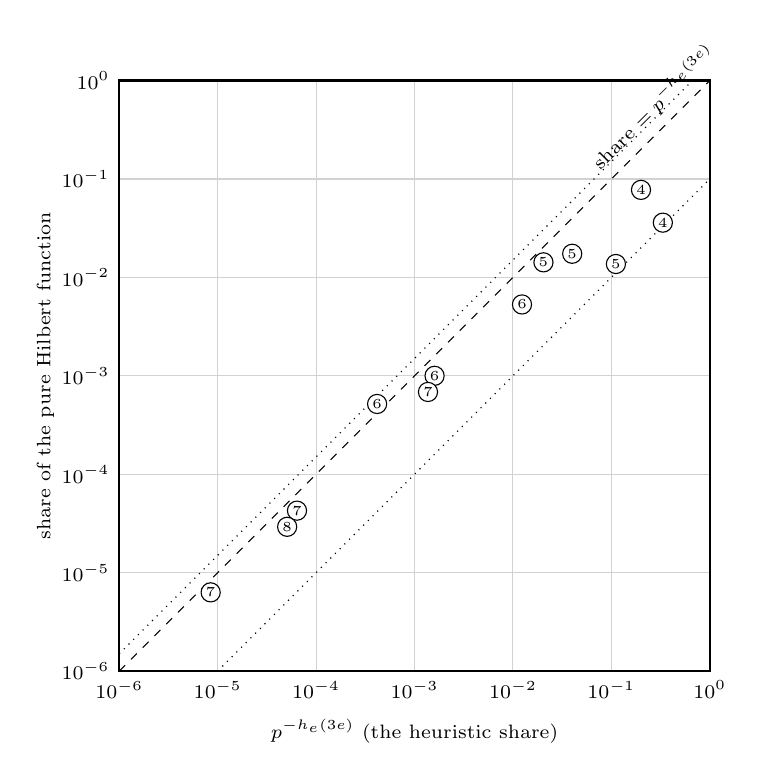
\begin{tikzpicture}[x=1.25cm,y=1.25cm,font=\scriptsize]
\draw[gray!35] (-6,-6) -- (-6,0); \draw[gray!35] (-6,-6) -- (0,-6);
\node[below] at (-6,-6) {$10^{-6}$}; \node[left] at (-6,-6) {$10^{-6}$};
\draw[gray!35] (-5,-6) -- (-5,0); \draw[gray!35] (-6,-5) -- (0,-5);
\node[below] at (-5,-6) {$10^{-5}$}; \node[left] at (-6,-5) {$10^{-5}$};
\draw[gray!35] (-4,-6) -- (-4,0); \draw[gray!35] (-6,-4) -- (0,-4);
\node[below] at (-4,-6) {$10^{-4}$}; \node[left] at (-6,-4) {$10^{-4}$};
\draw[gray!35] (-3,-6) -- (-3,0); \draw[gray!35] (-6,-3) -- (0,-3);
\node[below] at (-3,-6) {$10^{-3}$}; \node[left] at (-6,-3) {$10^{-3}$};
\draw[gray!35] (-2,-6) -- (-2,0); \draw[gray!35] (-6,-2) -- (0,-2);
\node[below] at (-2,-6) {$10^{-2}$}; \node[left] at (-6,-2) {$10^{-2}$};
\draw[gray!35] (-1,-6) -- (-1,0); \draw[gray!35] (-6,-1) -- (0,-1);
\node[below] at (-1,-6) {$10^{-1}$}; \node[left] at (-6,-1) {$10^{-1}$};
\draw[gray!35] (0,-6) -- (0,0); \draw[gray!35] (-6,0) -- (0,0);
\node[below] at (0,-6) {$10^{0}$}; \node[left] at (-6,0) {$10^{0}$};
\draw[thick] (-6,-6) rectangle (0,0);
\draw[dashed] (-6,-6) -- (0,0) node[pos=0.93,above,sloped]{share $=p^{-h_e(3e)}$};
\draw[dotted] (-5.000,-6.000) -- (0.000,-1.000);
\draw[dotted] (-6.000,-5.824) -- (-0.176,0.000);
\node[circle,draw,fill=white,inner sep=0.8pt,font=\tiny] at (-0.477,-1.444) {4};
\node[circle,draw,fill=white,inner sep=0.8pt,font=\tiny] at (-0.699,-1.111) {4};
\node[circle,draw,fill=white,inner sep=0.8pt,font=\tiny] at (-0.954,-1.864) {5};
\node[circle,draw,fill=white,inner sep=0.8pt,font=\tiny] at (-1.398,-1.760) {5};
\node[circle,draw,fill=white,inner sep=0.8pt,font=\tiny] at (-1.690,-1.847) {5};
\node[circle,draw,fill=white,inner sep=0.8pt,font=\tiny] at (-1.908,-2.275) {6};
\node[circle,draw,fill=white,inner sep=0.8pt,font=\tiny] at (-2.796,-3.000) {6};
\node[circle,draw,fill=white,inner sep=0.8pt,font=\tiny] at (-3.380,-3.286) {6};
\node[circle,draw,fill=white,inner sep=0.8pt,font=\tiny] at (-2.863,-3.164) {7};
\node[circle,draw,fill=white,inner sep=0.8pt,font=\tiny] at (-4.194,-4.370) {7};
\node[circle,draw,fill=white,inner sep=0.8pt,font=\tiny] at (-5.071,-5.200) {7};
\node[circle,draw,fill=white,inner sep=0.8pt,font=\tiny] at (-4.294,-4.534) {8};
\node[below=14pt] at (-3,-6) {$p^{-h_e(3e)}$ (the heuristic share)}; \node[rotate=90,above=20pt] at (-6,-3) {share of the pure Hilbert function};
\end{tikzpicture}

\caption{The share of members of $S(2;0,1)$ with the pure Hilbert function among the members examined, against the heuristic share $p^{-h_e(3e)}$ of the dimension count, on logarithmic axes, for the eleven pairs of families Q and C and the pair $(8,3)$ of family E where it is positive (each point is labelled by $e$); the dashed line is the equality and the dotted lines are $0.1$ and $1.5$ times it. All twelve points lie between the dotted lines.}
\label{fig:wcshare}
\end{figure}

\emph{The exclusion.} The \nwcNonAdm{} strata of family C that are not admissible hold no member with the pure Hilbert function among the \nwcNonAdmMembers{} members examined there, as Proposition~\ref{prop:strata} requires [MV]. In characteristic $p$ no member of a stratum whose modulus is divisible by $p$ has the rank $r$ in any pair of families Q and C (among \nwcPfourMembers{} members examined in those strata); Proposition~\ref{prop:pdivm} proves it for $p\le e-1$.

\emph{Degree $8$.} In the exploratory family E the search finds pure pairs over $\F_3$ (\nwcEEightThreePure{} pure members in \nwcEEightThreeStrataPure{} strata), over $\F_7$ (\nwcEEightSevenPure{} in the stratum $S(5;0,3)$, among $82{,}000$ random members; the other four strata are enumerated in full and hold no member with the pure Hilbert function) and over $\F_{13}$ (\nwcEEightThirteenPure{} in $S(7;0,1)$, the stratum of the linear family, among all \nwcEEightThirteenExamined{} members; for example $f=x^8+xy^7+2y^6z$, $g=y^8+x^6z$). It finds none in the strata examined over $\F_5$ (the five strata enumerated in full, \nwcEEightFiveExamined{} members, \nwcEEightFiveRankR{} of rank $r$, none with the pure Hilbert function) and none in $S(7;0,1)$ over $\F_{11}$ (all \nwcEEightElevenExamined{} members, \nwcEEightElevenRankR{} of rank $r$, none with the pure Hilbert function) [MV, complete enumerations over the prime field]; these are statements about those strata over $\F_p$. The stratum of the linear family holds pure members over $\F_{13}$ and none over $\F_{11}$ at $e=8$, which agrees with the rule of Section~\ref{sec:reslf}: pure members exactly when $2e-p\le3$ (the exclusion half is Corollary~\ref{cor:linstratum}; the other half is computed, not proved). The pure Hilbert function does not give the pure table: in $S(4;0,1)$ over $\F_3$ at $e=8$, \nwcEEightThreeHFFour{} members have the pure Hilbert function and none of the $40$ tables computed is pure, and in $S(4;0,3)$ $4$ of $40$ are [MV].

\emph{Cut enumerations.} The early stop at five pure members cut six enumerations: the strata $S(5;0,1)$ at $(6,11)$ (after $15{,}000$ of $17{,}689$ members), $S(7;0,3)$, $S(7;0,4)$ and $S(6;0,1)$ at $(7,11)$ (after $13{,}000$ of $17{,}568$, $17{,}000$ of $17{,}568$ and $17{,}000$ of $17{,}689$), $S(4;0,3)$ at $(7,3)$ (after $12{,}000$ of $14{,}641$) and $S(5;0,2)$ at $(7,7)$ (after $48{,}000$ of $160{,}000$); they hold pure members, so nothing is claimed about the rest of them. The computation used \nwcSeconds{} seconds of the allowed time.

\subsection{The pull-backs}
\label{sec:respull}

Table~\ref{tab:pullback} lists the \npbCases{} cases of Theorem~\ref{thm:scale} that were computed (computation \EXP{013}): seven pure pairs obtained by substituting an endomorphism of degree $d$ into a pure pair of degree $e'$ over $\F_3$, $\F_5$ or $\F_7$ (the pairs $(6,3)$, $(8,3)$, $(12,5)$, $(10,5)$, $(16,7)$, $(9,3)$, $(24,7)$) and three modules whose tables are not of the shape $(1,2,2,1)$. In every case both instruments give for the pull-back the Betti table of $M'$ with every degree multiplied by $d$, and the length $d^3$ times that of $M'$ [MV]; the pairs have lengths $216$, $512$, $1{,}728$, $1{,}000$, $4{,}096$, $729$ and \npbMaxLength{}. The script of the paper recomputes in its own arithmetic that $\varphi(z)$ is the commutator of $\varphi(x)$ and $\varphi(y)$, that the table of the pull-back is the scaled table of $M'$ in both instruments, that the length is $d^3$ times, and that the substitution of $\varphi$ into every generator of $M'$ gives the stored generators of the pull-back. The three modules with other tables are $U/(Ux+Uy^2)$ ($d=3$ and $d=6$) with the table $(1;1,1;1,1;1)$ on $(0;1,2;4,5;6)$, and $U/(Ux^2+Uxy+Uy^2+Uz)$ ($d=4$) with the table $(1;4;2,3;2)$ on $(0;2;3,4;5)$ and length $3$: their pull-backs have the same tables on the degrees multiplied by $3$, $6$ and $4$ (lengths $81$, $648$, $192$).

\begin{table}[htbp]
\centering\footnotesize
\begin{tabular}{@{}lrr>{\raggedright\arraybackslash}p{3.4cm}l>{\raggedright\arraybackslash}p{5.0cm}r@{}}
\toprule
case & $p$ & $d$ & module $M'$ & pull-back & pair of the pull-back, or the Betti numbers of $M'$ & length\\
\midrule
S1 & 3 & $3$ & $U/(U(x^{2}+y^{2}+yx)+U(x^{2}+yx-z))$ & $(6,3)$ & $f=x^{6} + x^{4}z - x^{3}yz + x^{3}y^{3} + x^{2}z^{2} + xyz^{2} - xy^{3}z + y^{2}z^{2} + y^{4}z + y^{6}$\newline $g=x^{6} + x^{4}z - x^{3}yz + x^{3}y^{3} + xyz^{2} + z^{3} + y^{2}z^{2} + y^{4}z$ & 216\\
S2 & 3 & $4$ & $U/(U(x^{2}+y^{2}+yx)+U(x^{2}+yx-z))$ & $(8,3)$ & $f=x^{8} + x^{4}y^{4} - x^{3}y^{3}z + y^{8}$\newline $g=x^{8} + x^{4}y^{4} + x^{3}y^{3}z - z^{4} + y^{4}z^{2}$ & 512\\
S3 & 5 & $6$ & $U/(Ux^{2}+Uy^{2})$ & $(12,5)$ & $f=x^{12} + 2x^{6}z^{3} + z^{6}$\newline $g=z^{6} + 2y^{6}z^{3} + y^{12}$ & 1728\\
S4 & 5 & $5$ & $U/(Ux^{2}+Uy^{2})$ & $(10,5)$ & $f=x^{10} + 2x^{5}yz^{2} + y^{2}z^{4}$\newline $g=x^{2}z^{4} + 2xy^{5}z^{2} + y^{10}$ & 1000\\
S5 & 7 & $8$ & $U/(Ux^{2}+Uy^{2})$ & $(16,7)$ & $f=x^{16} + 2x^{8}z^{4} + z^{8}$\newline $g=z^{8} + 2y^{8}z^{4} + y^{16}$ & 4096\\
S6 & 3 & $3$ & $U/(U(x^{3}+yz)+U(y^{3}+xz))$ & $(9,3)$ & $f=x^{9} - xz^{4}$\newline $g=-yz^{4} + y^{9}$ & 729\\
S7 & 7 & $8$ & $U/(Ux^{3}+Uy^{3})$ & $(24,7)$ & $f=x^{24} + 3x^{16}z^{4} + 3x^{8}z^{8} + z^{12}$\newline $g=z^{12} + 3y^{8}z^{8} + 3y^{16}z^{4} + y^{24}$ & 13824\\
T1 & 3 & $3$ & $U/(Ux+Uy^{2})$ & table & $\beta=1;1;1;1;1;1$ & 81\\
T2 & 5 & $6$ & $U/(Ux+Uy^{2})$ & table & $\beta=1;1;1;1;1;1$ & 648\\
T3 & 3 & $4$ & $U/(Ux^{2}+Uxy+Uy^{2}+Uz)$ & table & $\beta=1;4;2;3;2$ & 192\\
\bottomrule
\end{tabular}

\caption{The pull-backs computed: the case, the characteristic $p$, the degree $d$ of the endomorphism, the module $M'$, the pull-back (the pair $(e,p)$ of the new pure pair, or ``table'' for a module whose table is not pure) with the pair of forms over $\F_p$ obtained by substitution (or the Betti numbers of $M'$ in the order of the degrees), and the length of the pull-back; in every case the table of the pull-back is the table of $M'$ with degrees multiplied by $d$ in both instruments.}
\label{tab:pullback}
\end{table}

So the point $(1,2,2,1)$ of $(0,8,24,32)$ is realized over $U$ in characteristic $3$, that of $(0,12,36,48)$ in characteristic $5$, and those of $(0,16,48,64)$ and $(0,24,72,96)$ in characteristic $7$, by pairs of length $512$, $1{,}728$, $4{,}096$ and \npbMaxLength{}; in these pairs $(e,p)$ the characteristic divides neither $e$ nor $e-1$, and the pure pair comes from a pure pair of degree $2$ or $3$ by an endomorphism of degree $d\equiv0$ or $1$ modulo $p$ [MV, and Corollary~\ref{cor:scale1}]. The two cases outside the hypotheses behave as the theorem predicts: the pull-back of the power pair of degree $2$ along $x\mapsto x^5$, $y\mapsto y^5$ over $\F_5$ (an endomorphism with $\varphi(z)=0$, not of finite colength) is the power pair of degree $10$, which is not of finite length within the degree bound and has a Koszul syzygy in degree $20$; and the substitution of the pure pair of degree $5$ over $\F_7$ with non-central commutator into $x^2$ and $y^2$ gives a pair of degree $10$ that is not pure (length \npbNTwoLength{}, second syzygies in degrees $33$ and $34$) [MV]. The computations took \npbSeconds{} minutes; the table of the largest case, of length $13{,}824$, took $18$ minutes in the library and $6.5$ minutes in Singular. The experiment checks cases; the statement for every module and every $d\equiv0$ or $1\pmod p$ rests on the proof [D].

\subsection{The middle stratum and the strata at \texorpdfstring{$e=9$}{e=9}}
\label{sec:resmid}

The pairs $(x^e+b\,y^e,\ \Gamma(xy,z))$ of Section~\ref{sec:invariants} lie in the stratum $S(e;0,e/2)$ (the middle stratum). Computation \EXP{014} searched it at $e=8$, $10$ and $12$, and two strata at $e=9$: $S(5;0,4)$ and the stratum of the linear family, $S(8;0,1)$. Table~\ref{tab:mid} gives the cases, in three families: K (controls on settled pairs), V (the middle stratum at even $e$) and W (the strata at $e=9$). The computation is partly confirmed (two of its four predictions failed in part). The control $(7,11)$ in $S(4;0,3)$ failed as first designed, with the limit of $30{,}000$ random members: $559$ of rank $r$, $8$ with the pure Hilbert function, none pure, although pure members are known to exist there; about one member in $47{,}000$ is pure, so a sample of $30{,}000$ misses with probability about one half. The limit of that one control was raised to $300{,}000$ before any case of families V and W was computed, and under it the known answer holds: $232{,}000$ members examined before the early stop, $4{,}177$ of rank $r$, $39$ with the pure Hilbert function, $37$ tables, $5$ pure. The computation was run in two parts with the same runner: the gates and the controls first, then, after the amendment, the amended control, families V and W, the second instrument and the table, with one changed line (the budget of that control). The other eight controls gave their known answers with the original limit (pure members at $(4,3)$, $(4,5)$, $(6,5)$, $(6,7)$, $(6,11)$, $(5,7)$, $(7,5)$; no member of rank $r$ among the $160$ at $(6,3)$).

\begin{table}[htbp]
\centering\scriptsize
\begin{tabular}{@{}lrrlrrlrrr@{}}
\toprule
fam. & $e$ & $p$ & stratum & members & examined & mode & rank $r$ & pure $h_e$ & pure\\
\midrule
K & 4 & 3 & $S(4;0,2)$ & 52 & 52 & all members & 4 & 2 & 2\\
K & 4 & 5 & $S(4;0,2)$ & 186 & 186 & all members & 4 & 4 & 4\\
K & 5 & 7 & $S(3;0,2)$ & 160{,}000 & 16{,}000 & sampled & 901 & 82 & 6\\
K & 6 & 3 & $S(6;0,3)$ & 160 & 160 & all members & 0 & 0 & 0\\
K & 6 & 5 & $S(6;0,3)$ & 936 & 936 & all members & 24 & 8 & 8\\
K & 6 & 7 & $S(6;0,3)$ & 3{,}200 & 3{,}200 & all members & 588 & 12 & 11\\
K & 6 & 11 & $S(6;0,3)$ & 17{,}568 & 17{,}568 & all members & 1{,}600 & 340 & 4\\
K & 7 & 5 & $S(4;0,3)$ & 609{,}961 & 30{,}000 & sampled & 1{,}390 & 7 & 5\\
K & 7 & 11 & $S(4;0,3)$ & 259{,}371{,}025 & 232{,}000 & sampled & 4{,}177 & 39 & 5\\
V & 8 & 3 & $S(8;0,4)$ & 484 & 484 & all members & 36 & 0 & 0\\
V & 8 & 5 & $S(8;0,4)$ & 4{,}686 & 4{,}686 & all members & 436 & 4 & 4\\
V & 8 & 7 & $S(8;0,4)$ & 22{,}408 & 18{,}000 & in order, stopped early & 363 & 20 & 8\\
V & 8 & 11 & $S(8;0,4)$ & 193{,}260 & 104{,}000 & in order, stopped early & 16{,}333 & 6 & 5\\
V & 8 & 13 & $S(8;0,4)$ & 433{,}174 & 433{,}174 & all members & 34{,}524 & 156 & 3\\
V & 10 & 3 & $S(10;0,5)$ & 1{,}456 & 1{,}456 & all members & 30 & 20 & 11\\
V & 10 & 5 & $S(10;0,5)$ & 23{,}436 & 23{,}436 & all members & 0 & 0 & 0\\
V & 10 & 7 & $S(10;0,5)$ & 156{,}864 & 54{,}000 & in order, stopped early & 7{,}619 & 12 & 6\\
V & 10 & 11 & $S(10;0,5)$ & 2{,}125{,}872 & 280{,}000 & sampled & 43{,}513 & 6 & 6\\
V & 10 & 13 & $S(10;0,5)$ & 5{,}631{,}276 & 300{,}000 & sampled & 43{,}970 & 2 & 2\\
V & 12 & 5 & $S(12;0,6)$ & 117{,}186 & 44{,}000 & in order, stopped early & 7{,}423 & 16 & 9\\
V & 12 & 7 & $S(12;0,6)$ & 1{,}098{,}056 & 150{,}000 & sampled & 12{,}621 & 0 & 0\\
W & 9 & 5 & $S(5;0,4)$ & 15{,}256{,}836 & 300{,}000 & sampled & 0 & 0 & 0\\
W & 9 & 7 & $S(5;0,4)$ & 384{,}473{,}664 & 300{,}000 & sampled & 5{,}211 & 1 & 1\\
W & 9 & 11 & $S(5;0,4)$ & 31{,}384{,}248{,}336 & 300{,}000 & sampled & 1{,}598 & 0 & 0\\
W & 9 & 13 & $S(5;0,4)$ & 161{,}792{,}190{,}756 & 300{,}000 & sampled & 729 & 0 & 0\\
W & 9 & 11 & $S(8;0,1)$ & 17{,}689 & 17{,}689 & all members & 0 & 0 & 0\\
W & 9 & 13 & $S(8;0,1)$ & 33{,}489 & 33{,}489 & all members & 11{,}988 & 0 & 0\\
W & 9 & 17 & $S(8;0,1)$ & 94{,}249 & 20{,}000 & in order, stopped early & 10{,}369 & 5{,}990 & 5\\
\bottomrule
\end{tabular}

\caption{The cases of the search in the middle stratum and at $e=9$: the family (K controls, V middle stratum, W the strata at $e=9$), $(e,p)$, the stratum, the number of members, the number examined, whether all members were taken, the enumeration was cut by the early stop or the members were sampled, the members of rank $r$, with the pure Hilbert function and with the pure Betti table.}
\label{tab:mid}
\end{table}

\emph{Even $e$.} The middle stratum holds pure pairs over $\F_p$ at $e=8$ for $p=5,7,11,13$ (all of length $512$), at $e=10$ for $p=3,7,11,13$ (length $1{,}000$) and at $e=12$ for $p=5$ (length $1{,}728$); Table~\ref{tab:midpairs} prints one pair for each, with the second form a polynomial in $xy$ and $z$ and the first of the form $x^e+b\,y^e$, and the script recomputes the Hilbert function, the length and the rank of $\mu_{3e}$ of each pair with $e\le10$ and checks the stratum of every pair. With the pair over $\F_3$ of Section~\ref{sec:respull} this gives a pure pair of degree $8$ over $\F_p$ for every odd prime $p$ below $16$. The stratum holds no pure pair over $\F_3$ at $e=8$ (all $484$ members examined, $36$ of rank $r$, none with the pure Hilbert function), and at $(12,7)$ none was found ($150{,}000$ random members of $1{,}098{,}056$, \nmidTwelveSevenRankR{} of rank $r$, none with the pure Hilbert function; the stratum was sampled). At $(10,5)$ no member has the rank $r$ (all $23{,}436$ members examined), as Proposition~\ref{prop:pdivm} explains for the strata whose modulus is divisible by $p$. By complete enumeration over the prime field the stratum $S(8;0,4)$ holds no pure pair over $\F_3$, $S(10;0,5)$ holds no member of rank $r$ over $\F_5$, and $S(8;0,1)$ holds no pure pair over $\F_{11}$ and none over $\F_{13}$ at $e=9$ [MV]; these statements concern one stratum over the prime field.

\begin{table}[htbp]
\centering\footnotesize
\begin{tabular}{@{}ll>{\raggedright\arraybackslash}p{6.4cm}r@{}}
\toprule
$(e,p)$ & stratum & forms over $\F_p$ & length\\
\midrule
$(8,5)$ & $S(8;0,4)$ & $f=x^{8} + y^{8}$\newline $g=x^{4}y^{4} + 2x^{3}y^{3}z - x^{2}y^{2}z^{2} + xyz^{3} + 2z^{4}$ & 512\\
$(8,7)$ & $S(8;0,4)$ & $f=x^{8} + y^{8}$\newline $g=x^{4}y^{4} - x^{3}y^{3}z + x^{2}y^{2}z^{2} + xyz^{3} + 2z^{4}$ & 512\\
$(8,11)$ & $S(8;0,4)$ & $f=x^{8} + y^{8}$\newline $g=x^{4}y^{4} + 3x^{3}y^{3}z + 5x^{2}y^{2}z^{2} + 3xyz^{3} + 2z^{4}$ & 512\\
$(8,13)$ & $S(8;0,4)$ & $f=x^{8} + y^{8}$\newline $g=x^{4}y^{4} + 5x^{3}y^{3}z + 3x^{2}y^{2}z^{2} + 5xyz^{3} + 6z^{4}$ & 512\\
$(10,3)$ & $S(10;0,5)$ & $f=x^{10} + y^{10}$\newline $g=x^{5}y^{5} + x^{4}y^{4}z + z^{5}$ & 1000\\
$(10,7)$ & $S(10;0,5)$ & $f=x^{10} + y^{10}$\newline $g=x^{5}y^{5} + x^{4}y^{4}z + x^{3}y^{3}z^{2} - x^{2}y^{2}z^{3} - xyz^{4} - 3z^{5}$ & 1000\\
$(10,11)$ & $S(10;0,5)$ & $f=-x^{10} - 4y^{10}$\newline $g=4x^{5}y^{5} + 2x^{4}y^{4}z + 4x^{3}y^{3}z^{2} - 3x^{2}y^{2}z^{3} + 4xyz^{4} + 2z^{5}$ & 1000\\
$(10,13)$ & $S(10;0,5)$ & $f=-5x^{10} + 4y^{10}$\newline $g=x^{5}y^{5} - 6x^{4}y^{4}z - 6x^{3}y^{3}z^{2} - 3x^{2}y^{2}z^{3} + 3xyz^{4} - 6z^{5}$ & 1000\\
$(12,5)$ & $S(12;0,6)$ & $f=x^{12} + y^{12}$\newline $g=x^{6}y^{6} + 2x^{5}y^{5}z + x^{4}y^{4}z^{2} + 2x^{3}y^{3}z^{3} + 2x^{2}y^{2}z^{4} + xyz^{5} + 2z^{6}$ & 1728\\
$(9,7)$ & $S(5;0,4)$ & $f=-3x^{9} - 2x^{4}y^{5} - x^{3}y^{4}z + 3x^{2}y^{3}z^{2} - 2xy^{2}z^{3} + 3yz^{4}$\newline $g=x^{5}y^{4} + 3x^{4}y^{3}z + 2x^{3}y^{2}z^{2} + 2x^{2}yz^{3} - xz^{4} - 3y^{9}$ & 729\\
$(9,17)$ & $S(8;0,1)$ & $f=x^{9} + xy^{8}$\newline $g=x^{7}z + y^{9}$ & 729\\
\bottomrule
\end{tabular}

\caption{One pure pair found in the middle stratum or in a stratum at $e=9$ for each pair $(e,p)$ settled by that search: the stratum, the forms over $\F_p$ (coefficients of least absolute value) and the length of $U/(Uf+Ug)$ (equal to $e^3$); the script checks the stratum of each pair and recomputes the Hilbert function, the length and the rank of $\mu_{3e}$ for $e\le10$, and both instruments give the Betti table $(1,2,2,1)$ on $(0,e,3e,4e)$.}
\label{tab:midpairs}
\end{table}

\emph{Odd $e$.} At $e=9$ the stratum $S(5;0,4)$ holds a pure pair over $\F_7$ (one among $300{,}000$ random members, \nmidNineSevenORankR{} of rank $r$, one with the pure Hilbert function) and none was found over $\F_{11}$ and $\F_{13}$ ($300{,}000$ random members each, \nmidNineElevenORankR{} and \nmidNineThirteenORankR{} of rank $r$, none with the pure Hilbert function); over $\F_5$ no member of the sample has the rank $r$. The stratum $S(8;0,1)$ holds a pure pair over $\F_{17}$ (the enumeration stopped after $20{,}000$ of $94{,}249$ members with $5$ pure members, \nmidNineSeventeenLRankR{} of rank $r$, \nmidNineSeventeenLPureHF{} with the pure Hilbert function) and none over $\F_{11}$ and $\F_{13}$, which is the outcome that the rule of the linear family gives ($2e-p=1$ against $7$ and $5$); the absence is Corollary~\ref{cor:linstratum}, and the two outcomes were recorded before they were computed. The pairs $(9,5)$, $(9,11)$ and $(9,13)$ were open at the time of this computation and are settled by the strata of Section~\ref{sec:reslinrule}; $(9,3)$ is settled by Theorem~\ref{thm:central}, and $(9,7)$ and $(9,17)$ by the pairs above.

\emph{The Hilbert function and the table.} In $S(6;0,3)$ over $\F_{11}$ and in $S(8;0,4)$ over $\F_{13}$ most members with the pure Hilbert function have another Betti table ($4$ pure of $40$ tables computed, and $3$ of $40$), so the pure Hilbert function alone does not give a pure pair in these strata; this is consistent with Remark~\ref{rem:invariants}(5): by Theorem~\ref{thm:betti} a member of the shape of Section~\ref{sec:invariants} with the pure Hilbert function and another table does not satisfy (C). An independent count of the forms $\Gamma$ that satisfy (C) and the conditions of Theorem~\ref{thm:inv}(b), evaluated for every monic $\Gamma$ over the prime field, gives $1$, $4$, $1$, $1$ forms at $(8,5)$, $(8,7)$, $(8,11)$, $(8,13)$, and these are the forms of the pure members found here (compared after rewriting $g$ in $\xi=xy$ and $z$: for example $\Gamma=\xi^4+3\xi^3z+\xi^2z^2+2z^4$ over $\F_5$ and $\xi^4+11\xi^3z+3\xi^2z^2+11\xi z^3+6z^4$ over $\F_{13}$); at $(8,13)$, $12$ of the $156$ members with the pure Hilbert function carry that form [U as archived evidence]. These forms are exactly the forms with (C) and the congruence~\eqref{eq:cong} of Theorem~\ref{thm:cong}, compared by hand after rewriting $g$ in $\xi$ and $z$ [U as archived evidence]. The computation took \nmidSeconds{} seconds of the allowed time.

\subsection{The rule of the linear family for \texorpdfstring{$e=10$ to $13$}{e=10 to 13}, and the pairs at \texorpdfstring{$e=9$}{e=9}}
\label{sec:reslinrule}

Computation \EXP{015} examines the stratum of the linear family, $S(e-1;0,1)$, at twelve of the fourteen pairs $(e,p)$ with $e=10$ to $13$ and $e<p<2e$ (the two others, $(12,13)$ and $(13,17)$, have $2e-p=11$ and $9$ and are covered by Corollary~\ref{cor:linstratum}; Table~\ref{tab:linrule}), and the strata that remained at the three pairs $(9,5)$, $(9,11)$, $(9,13)$ that were open. Controls with known answers (the pure pairs of the stratum of the linear family at $(9,17)$ and $(8,13)$ and the absence at $(9,13)$ and $(8,11)$) are part of the computation and are listed in its artifact [MV]. The prediction fixed before the run was that the stratum holds a pure member exactly when $2e-p\le3$ (confidence $0.7$ for the twelve outcomes together), with the exclusion half supported by Corollary~\ref{cor:linstratum}, whose statement was recorded before the results were read.

\begin{table}[htbp]
\centering\footnotesize
\begin{tabular}{@{}rrrrrlrrr@{}}
\toprule
$e$ & $p$ & $2e-p$ & members & examined & mode & rank $r$ & pure $h_e$ & pure\\
\midrule
10 & 11 & 9 & 17{,}689 & 17{,}689 & all & 0 & 0 & 0\\
10 & 13 & 7 & 33{,}489 & 33{,}489 & all & 0 & 0 & 0\\
10 & 17 & 3 & 94{,}249 & 28{,}000 & in order, stopped early & 12{,}704 & 8{,}532 & 5\\
10 & 19 & 1 & 145{,}161 & 24{,}000 & sampled & 15{,}928 & 9{,}326 & 7\\
11 & 13 & 9 & 33{,}489 & 33{,}489 & all & 0 & 0 & 0\\
11 & 17 & 5 & 94{,}249 & 94{,}249 & all & 36{,}208 & 0 & 0\\
11 & 19 & 3 & 145{,}161 & 24{,}000 & sampled & 13{,}342 & 8{,}951 & 15\\
12 & 17 & 7 & 94{,}249 & 94{,}249 & all & 0 & 0 & 0\\
12 & 19 & 5 & 145{,}161 & 100{,}000 & sampled & 39{,}403 & 0 & 0\\
12 & 23 & 1 & 305{,}809 & 24{,}000 & sampled & 16{,}318 & 9{,}754 & 14\\
13 & 19 & 7 & 145{,}161 & 100{,}000 & sampled & 0 & 0 & 0\\
13 & 23 & 3 & 305{,}809 & 24{,}000 & sampled & 13{,}925 & 9{,}442 & 14\\
\bottomrule
\end{tabular}

\caption{The stratum of the linear family at the twelve pairs $(e,p)$ with $e=10$ to $13$: $e$, $p$, $2e-p$, the number of members ($N$), the number examined, whether all members were taken, the enumeration was cut by the early stop or the members were sampled, the members of rank $r$, with the pure Hilbert function and with the pure Betti table.}
\label{tab:linrule}
\end{table}

The stratum holds pure members at $(10,17)$, $(10,19)$, $(11,19)$, $(12,23)$ and $(13,23)$ (\nlinrTenSeventeenPure, \nlinrTenNineteenPure, \nlinrElevenNineteenPure, \nlinrTwelveTwentyThreePure{} and \nlinrThirteenTwentyThreePure{} pure members; Table~\ref{tab:linrule} gives the members with the pure Hilbert function), where $2e-p\in\{1,3\}$. It holds no member with the pure Hilbert function at $(10,11)$, $(10,13)$, $(11,13)$, $(11,17)$, $(12,17)$ and at $(12,19)$, $(13,19)$ (the members examined are in Table~\ref{tab:linrule}). The number of members of rank $r$ is $0$ at the pairs with $2e-p\ge7$ and \nlinrElevenSeventeenRankR{} and \nlinrTwelveNineteenRankR{} at $(11,17)$ and $(12,19)$, where $2e-p=5$; where $2e-p\ge5$ the absence of pure pairs follows from Corollary~\ref{cor:linstratum}, not from the sample. Table~\ref{tab:rule} puts the twelve pairs together with the twelve of Sections~\ref{sec:reslf}, \ref{sec:resstrata} and~\ref{sec:resmid}: in all $24$ computed pairs with $4\le e\le13$ and $e<p<2e$ (the two pairs not computed are excluded by the corollary) the stratum holds pure members exactly when $2e-p\le3$. The half ``none when $2e-p\ge5$'' is Corollary~\ref{cor:linstratum}; the half ``pure members when $p=2e-3$ or $2e-1$'' is computed on the thirteen pairs of the table with $2e-p\le3$ and is not proved [MV].

\begin{table}[htbp]
\centering\footnotesize
\begin{tabular}{@{}rrrlrrl@{}}
\toprule
$e$ & $p$ & $2e-p$ & computation & members examined & pure & reading\\
\midrule
4 & 5 & 3 & EXP-009 & 625 & 95 & pure members\\
4 & 7 & 1 & EXP-009 & 2{,}401 & 98 & pure members\\
5 & 7 & 3 & EXP-009 & 2{,}401 & 110 & pure members\\
6 & 7 & 5 & EXP-009 & 2{,}401 & 0 & none\\
6 & 11 & 1 & EXP-009 & 14{,}641 & 99 & pure members\\
7 & 11 & 3 & EXP-009 & 14{,}641 & 111 & pure members\\
7 & 13 & 1 & EXP-009 & 28{,}561 & 111 & pure members\\
8 & 11 & 5 & EXP-010 & 17{,}689 & 0 & none\\
8 & 13 & 3 & EXP-010 & 33{,}489 & 8 & pure members\\
9 & 11 & 7 & EXP-014 & 17{,}689 & 0 & none\\
9 & 13 & 5 & EXP-014 & 33{,}489 & 0 & none\\
9 & 17 & 1 & EXP-014 & 20{,}000 & 5 & pure members\\
10 & 11 & 9 & EXP-015 & 17{,}689 & 0 & none\\
10 & 13 & 7 & EXP-015 & 33{,}489 & 0 & none\\
10 & 17 & 3 & EXP-015 & 28{,}000 & 5 & pure members\\
10 & 19 & 1 & EXP-015 & 24{,}000 & 7 & pure members\\
11 & 13 & 9 & EXP-015 & 33{,}489 & 0 & none\\
11 & 17 & 5 & EXP-015 & 94{,}249 & 0 & none\\
11 & 19 & 3 & EXP-015 & 24{,}000 & 15 & pure members\\
12 & 17 & 7 & EXP-015 & 94{,}249 & 0 & none\\
12 & 19 & 5 & EXP-015 & 100{,}000 & 0 & none\\
12 & 23 & 1 & EXP-015 & 24{,}000 & 14 & pure members\\
13 & 19 & 7 & EXP-015 & 100{,}000 & 0 & none\\
13 & 23 & 3 & EXP-015 & 24{,}000 & 14 & pure members\\
\bottomrule
\end{tabular}

\caption{The stratum $S(e-1;0,1)$ (the linear family) at the \nrulePairs{} pairs $(e,p)$ with $4\le e\le13$ and $e<p<2e$ that were computed: $2e-p$, the computation, the members examined and the pure members; pure members occur exactly when $2e-p\le3$.}
\label{tab:rule}
\end{table}

\emph{The pairs at $e=9$.} Each of $(9,5)$, $(9,11)$, $(9,13)$ has a pure pair over $\F_p$ (Table~\ref{tab:linrulepairs}): at $(9,5)$ in the stratum $S(4;0,1)$ (\nlinrNineFiveNineAll{} members examined in the twelve strata of the pair), at $(9,11)$ in $S(7;0,2)$ and in $S(6;0,3)$, and at $(9,13)$ in $S(7;0,2)$ and in $S(6;0,3)$; the pairs and their lengths are in Table~\ref{tab:linrulepairs}. The strata at $(9,5)$ that the exclusions of Section~\ref{sec:wzero} leave in the refined list are counted in Table~\ref{tab:wzleft}, and the pure pair lies in one of them, $S(4;0,1)$; no member with the pure Hilbert function was found in the strata that Corollary~\ref{cor:wzstrata} excludes (\nwzExcludedFifteen{} strata at the three pairs; the predictions of the note were recorded before the results were read and all held). So $e=9$ is complete: with the criterion ($p=3$), Section~\ref{sec:resmid} ($p=7$), the stratum of the linear family ($p=17$) and these pairs, every odd prime below $18$ has a pure pair of degree $9$ over $\F_p$ [MV].

\begin{table}[htbp]
\centering\footnotesize
\begin{tabular}{@{}ll>{\raggedright\arraybackslash}p{6.4cm}r@{}}
\toprule
$(e,p)$ & stratum & forms over $\F_p$ & length\\
\midrule
$(9,5)$ & $S(4;0,1)$ & $f=-x^{9} + x^{5}y^{4} + x^{3}y^{2}z^{2} - 2x^{2}yz^{3} + 2xz^{4} - 2xy^{8} + 2y^{7}z$\newline $g=-2x^{8}y - 2x^{7}z + x^{4}y^{5} - 2x^{2}y^{3}z^{2} - xy^{2}z^{3} - 2yz^{4} + y^{9}$ & 729\\
$(9,11)$ & $S(7;0,2)$ & $f=-5x^{9} + 5x^{2}y^{7} - 4y^{5}z^{2}$\newline $g=-4x^{7}y^{2} + 2x^{6}yz - 4x^{5}z^{2} + 2y^{9}$ & 729\\
$(9,11)$ & $S(6;0,3)$ & $f=-x^{9} - x^{2}y^{5}z - 2xy^{4}z^{2} + 2y^{3}z^{3}$\newline $g=2x^{6}y^{3} - 4x^{5}y^{2}z + 4x^{3}z^{3} + 3y^{9}$ & 729\\
$(9,13)$ & $S(7;0,2)$ & $f=2x^{9} + 3x^{2}y^{7} - 4xy^{6}z + 6y^{5}z^{2}$\newline $g=-3x^{7}y^{2} - 6x^{6}yz + x^{5}z^{2} + 5y^{9}$ & 729\\
$(9,13)$ & $S(6;0,3)$ & $f=-x^{9} - x^{3}y^{6} + 5x^{2}y^{5}z + xy^{4}z^{2} - 4y^{3}z^{3}$\newline $g=-5x^{6}y^{3} - 4x^{3}z^{3} + 3y^{9}$ & 729\\
$(10,17)$ & $S(9;0,1)$ & $f=x^{10} + xy^{9} + 2y^{8}z$\newline $g=3x^{8}z + y^{10}$ & 1000\\
$(10,19)$ & $S(9;0,1)$ & $f=7x^{10} + 4xy^{9} + y^{8}z$\newline $g=7x^{9}y + 8x^{8}z + y^{10}$ & 1000\\
$(11,19)$ & $S(10;0,1)$ & $f=6x^{11} - 7xy^{10} - 8y^{9}z$\newline $g=5x^{10}y + 9x^{9}z + 3y^{11}$ & 1331\\
$(12,23)$ & $S(11;0,1)$ & $f=-7x^{12} + xy^{11} + 5y^{10}z$\newline $g=9x^{11}y + 6x^{10}z - 9y^{12}$ & 1728\\
$(13,23)$ & $S(12;0,1)$ & $f=5x^{13} - xy^{12} + 10y^{11}z$\newline $g=-5x^{12}y - x^{11}z - 9y^{13}$ & 2197\\
\bottomrule
\end{tabular}

\caption{Pure pairs found by \EXP{015}: the three pairs at $e=9$ (the strata $S(4;0,1)$ at $p=5$, $S(7;0,2)$ and $S(6;0,3)$ at $p=11$ and $13$) and one pair at each of the pairs $(10,17)$, $(10,19)$, $(11,19)$, $(12,23)$, $(13,23)$ in the stratum of the linear family: the stratum, the forms over $\F_p$ and the length of $U/(Uf+Ug)$; the script checks the stratum of each pair and recomputes the Hilbert function, the length and the rank of $\mu_{3e}$ for $e\le11$, and both instruments give the table $(1,2,2,1)$ on $(0,e,3e,4e)$.}
\label{tab:linrulepairs}
\end{table}

The strata that hold the pure pairs at $(9,11)$ and $(9,13)$ are the pairs $x^9+\alpha(xy,z)y^t$, $y^9+\beta(xy,z)x^t$ with $t=5$ ($S(7;0,2)$) and $t=3$ ($S(6;0,3)$); the linear family is $t=7$ and the stratum of the central pairs $t=1$. This is an observation on the strata of this computation and of Section~\ref{sec:resmid}; the exclusions are proved (Corollary~\ref{cor:wzstrata}), the reading in terms of $t$ is not. One deviation is recorded: the rank routine of the computation \EXP{010} raised an overflow error at $e=13$ (an exact coefficient exceeded the range of a machine integer), and the run was resumed with a replacement of that function that reduces each coefficient modulo $p$ before storing it (the same tensor modulo $p$); the earlier computations are not affected, because an entry that does not fit raises an error instead of wrapping, and none was raised. The computation used \nlinrSeconds{} seconds of the allowed time.

\subsection{A filter in the stratum of the central pairs}
\label{sec:resfilter}

For odd $e$ and $s=(e-1)/2$ the stratum $S((e+1)/2;0,(e-1)/2)$ consists of the pairs $f=x^e+\alpha(\xi,z)\,y$, $g=y^e+\beta(\xi,z)\,x$ with $\alpha,\beta$ forms of degree $s$ in $\xi=xy$ and $z$ (up to scalars on $f$ and $g$). It holds the central pairs and the pure pairs found by the searches of Sections~\ref{sec:resstrata} and~\ref{sec:resmid} for odd $e$ in small characteristic. Computation \EXP{017} searches it at $(9,11)$ and $(9,13)$ and, exploratory, at $(11,7)$ and $(13,5)$ through a \emph{filter}, which is defined here exactly as it was fixed before the computation and is \textbf{not proved}. With $z=1$, $A_n(\xi)=\xi(\xi+1)\cdots(\xi+n-1)$ and $\Delta=\alpha(\xi)\beta(\xi+e-1)-A_{e-1}(\xi)$, $X=(\xi-2)\Delta(\xi-e-1)$, $X'=(\xi+e)\Delta(\xi+e+1)$:
\begin{description}
\item[(F0)] $\Delta$ has degree $2s$ and is coprime to $X$ and to $X'$;
\item[(F1)] $X'\alpha\equiv cX$ modulo $\Delta$ for a polynomial $c$ of degree at most $s$;
\item[(F2)] $X\beta(\xi+e-1)\equiv c'X'$ modulo $\Delta$ for a polynomial $c'$ of degree at most $s$;
\item[(F3)] $cc'$ is not equal to $A_{e-1}$.
\end{description}
The filter was read off computed cases on settled pairs and is used only to choose which members to compute in $U$: a member that passes need not be pure, and nothing is computed in $U$ for the members that fail it. Its evidence before the computation is that the \nstmPure{} pure members of this stratum stored by the searches of Sections~\ref{sec:resstrata} and~\ref{sec:resmid} satisfy (F0) to (F3) [MV: recomputed from the stored members of \EXP{010} and \EXP{014}; \nstmFailFZero{} of the \nstmOther{} fail (F0) and \nstmFailFThree{} fail (F3)]. Conditions (F1) and (F2) are $2(s-1)=e-3$ conditions on the $2s+1=e$ parameters of $(\alpha,\beta)$ up to the scaling $(\alpha,\beta)\mapsto(t\alpha,\beta/t)$ that comes from $x\mapsto\lambda x$, $y\mapsto\mu y$, which suggests a density of about $p^{-(e-3)}$ among all members; the density is reported as measured, not proved.

\begin{table}[htbp]
\centering\scriptsize
\begin{tabular}{@{}lrrrrrrrrrrr@{}}
\toprule
fam. & $e$ & $p$ & examined & (F0) & (F1) & (F2) & (F3) & pure $h_e$ & tables & pure & share/$p^{-(e-3)}$\\
\midrule
K & 5 & 7 & 200{,}000 & 16{,}946 & 16{,}946 & 2{,}212 & 1{,}027 & 1{,}027 & 14 & 14 & 0.25\\
K & 7 & 5 & 1{,}310{,}720 & 14{,}182 & 14{,}182 & 1{,}555 & 594 & 594 & 15 & 15 & 0.28\\
K & 7 & 11 & 1{,}376{,}256 & 7{,}573 & 7{,}573 & 124 & 44 & 44 & 16 & 16 & 0.47\\
K & 9 & 7 & 2{,}883{,}584 & 2{,}975 & 2{,}975 & 35 & 13 & 13 & 9 & 9 & 0.53\\
Q & 9 & 11 & 17{,}039{,}360 & 8{,}740 & 8{,}740 & 26 & 5 & 5 & 5 & 5 & 0.52\\
Q & 9 & 13 & 38{,}862{,}848 & 12{,}374 & 12{,}374 & 16 & 5 & 5 & 5 & 5 & 0.62\\
X & 11 & 7 & 25{,}165{,}824 & 4{,}064 & 4{,}064 & 14 & 6 & 6 & 6 & 6 & 1.37\\
X & 13 & 5 & 25{,}296{,}896 & 3{,}043 & 3{,}043 & 17 & 5 & 5 & 5 & 5 & 1.93\\
\bottomrule
\end{tabular}

\caption{The filter of Section~\ref{sec:resfilter} in the stratum of the central pairs: the family (K controls on settled pairs, Q the question at $e=9$, X exploratory), $(e,p)$, the random members examined, those that pass (F0), (F0) and (F1), (F0) to (F2), (F0) to (F3), those with the pure Hilbert function, the Betti tables computed and the pure ones, and the ratio of the share that passes to $p^{-(e-3)}$.}
\label{tab:filter}
\end{table}

\emph{Results.} Table~\ref{tab:filter} gives the eight cases. In each, every member that passes the filter has the pure Hilbert function (\nfltPassed{} members in all) and every Betti table computed is pure (\nfltTables{} tables); the last column of Table~\ref{tab:filter} gives the share of members that pass relative to $p^{-(e-3)}$. The pairs found are pure pairs over $\F_p$ at $(9,11)$ (\nfltNineElevenPass{} members pass among \nfltNineElevenExamined{} random members), $(9,13)$ (\nfltNineThirteenPass{} among \nfltNineThirteenExamined{}), $(11,7)$ (\nfltElevenSevenPass{} among \nfltElevenSevenExamined{}) and $(13,5)$ (\nfltThirteenFivePass{} among \nfltThirteenFiveExamined{}) (Table~\ref{tab:filterpairs}): the point $(1,2,2,1)$ of $(0,11,33,44)$ is realized over $\F_7$ (length $1{,}331$) and that of $(0,13,39,52)$ over $\F_5$ (length $2{,}197$), pairs that no theorem (the characteristic divides neither $e$ nor $e-1$ and no pull-back applies) and no earlier search had reached [MV].

\begin{table}[htbp]
\centering\footnotesize
\begin{tabular}{@{}ll>{\raggedright\arraybackslash}p{6.4cm}r@{}}
\toprule
$(e,p)$ & stratum & forms over $\F_p$ & length\\
\midrule
$(9,11)$ & $S(5;0,4)$ & $f=x^{9} + 4x^{4}y^{5} - 2x^{3}y^{4}z - 2x^{2}y^{3}z^{2} + 4xy^{2}z^{3}$\newline $g=-x^{5}y^{4} + 4x^{4}y^{3}z - 3x^{3}y^{2}z^{2} + 4x^{2}yz^{3} + 3xz^{4} + y^{9}$ & 729\\
$(9,13)$ & $S(5;0,4)$ & $f=x^{9} + x^{4}y^{5} - x^{2}y^{3}z^{2} - 6xy^{2}z^{3} - 5yz^{4}$\newline $g=-6x^{5}y^{4} + 5x^{4}y^{3}z - 6x^{3}y^{2}z^{2} - 5xz^{4} + y^{9}$ & 729\\
$(11,7)$ & $S(6;0,5)$ & $f=x^{11} + 2x^{5}y^{6} - x^{4}y^{5}z + 2x^{3}y^{4}z^{2} + 3x^{2}y^{3}z^{3} - 3xy^{2}z^{4} + 2yz^{5}$\newline $g=-x^{6}y^{5} - x^{5}y^{4}z + 2x^{3}y^{2}z^{3} + 2x^{2}yz^{4} - 2xz^{5} + y^{11}$ & 1331\\
$(13,5)$ & $S(7;0,6)$ & $f=x^{13} - 2x^{6}y^{7} + x^{5}y^{6}z - 2x^{3}y^{4}z^{3} - x^{2}y^{3}z^{4} + 2xy^{2}z^{5} + 2yz^{6}$\newline $g=x^{7}y^{6} + 2x^{6}y^{5}z + x^{5}y^{4}z^{2} + x^{4}y^{3}z^{3} + 2x^{2}yz^{5} + 2xz^{6} + y^{13}$ & 2197\\
\bottomrule
\end{tabular}

\caption{Pure pairs found through the filter: the pair $(e,p)$, the stratum $S((e+1)/2;0,(e-1)/2)$, the forms over $\F_p$ and the length of $U/(Uf+Ug)$; the script checks the stratum of each pair and recomputes the Hilbert function, the length and the rank of $\mu_{3e}$, and both instruments give the table $(1,2,2,1)$ on $(0,e,3e,4e)$.}
\label{tab:filterpairs}
\end{table}

\emph{What the filter is.} All $1{,}699$ members that pass have the pure Hilbert function and all $75$ tables computed are pure; of the \nstmTabled{} members of the stratum stored by the searches of Sections~\ref{sec:resstrata} and~\ref{sec:resmid} with a computed table, at \nstmPairs{} pairs, the \nstmPure{} pure ones pass and the \nstmOther{} others do not [MV: recomputed from the stored members of \EXP{010} and \EXP{014}; \nstmFailFZero{} of the \nstmOther{} fail (F0) and \nstmFailFThree{} fail (F3)]. This is an observation, not a theorem: that a member is pure exactly when it passes (F0) to (F3) is supported in one direction by $75$ tables and $1{,}699$ Hilbert functions, and in the other by the \nstmOther{} stored members with another table, none of which passes the filter; no member that fails the filter was tabled in this computation. The question the filter leaves is whether it is exact (a criterion for purity in this stratum, in the manner of Theorem~\ref{thm:cong} for the middle stratum) or only a necessary condition that is almost always sufficient; a derivation with proofs for this stratum, and for the pairs $x^e+\alpha(xy,z)\,y^t$, $y^e+\beta(xy,z)\,x^t$ with other $t$, is not part of this paper. The density $p^{-(e-3)}$ is reported as measured. The case $(13,5)$ first stopped on the overflow error of the rank routine mentioned above and was run again from its start with the same replacement. The computation used \nfltSeconds{} seconds of the allowed time.

\subsection{Lists of forms by one congruence}
\label{sec:reslists}

For even $e$ the pairs $f=x^e+y^e$, $g=\Gamma(xy,z)$ with $\Gamma$ a monic form of degree $e/2$ in $\xi=xy$ and $z$ are those of Theorem~\ref{thm:cong}: under the hypothesis (C) the module is pure exactly when $\Gamma$ satisfies one congruence, and the pure Betti table follows (Theorem~\ref{thm:betti}). Computation \EXP{016} lists, at the $25$ pairs over prime fields and the three extension fields of Table~\ref{tab:lists}, every monic $\Gamma(\xi,1)$ over $\F_p$ that satisfies (C) and the congruence, by complete enumeration of the $p^{e/2}$ forms except where Table~\ref{tab:lists} says otherwise, and the same at $e=8$ and $e=14$ over $\F_9$ and at $e=6$ over $\F_{169}$. The congruence is first tested by a fast routine on blocks of forms and then by the exact test; the two agreed on every form that passed the fast test (\nlstFastNotExact{} disagreements). Controls with known answers precede it (the lists of the pairs of Sections~\ref{sec:resmid} and~\ref{sec:reslf} at $e\le10$, with the sizes fixed before the computation), and every listed form that was checked in $U$, \nlstVerified{} in all, has length $e^3$ and the table $(1,2,2,1)$ on $(0,e,3e,4e)$ in the first instrument and the same table in the second (Singular with Plural) [MV].

\begin{table}[htbp]
\centering\footnotesize
\begin{tabular}{@{}rlrrrl@{}}
\toprule
$e$ & field & forms & with the congruence & list & enumeration\\
\midrule
6 & $\F_{169}$ & 4{,}826{,}809 & 307 & 148 & complete\\
8 & $\F_{9}$ & 6{,}561 & 198 & 0 & complete\\
10 & $\F_{3}$ & 243 & 28 & 10 & complete\\
10 & $\F_{7}$ & 16{,}807 & 191 & 6 & complete\\
10 & $\F_{11}$ & 161{,}051 & 1{,}075 & 4 & complete\\
10 & $\F_{13}$ & 371{,}293 & 893 & 4 & complete\\
10 & $\F_{17}$ & 1{,}419{,}857 & 369 & 2 & complete\\
10 & $\F_{19}$ & 2{,}476{,}099 & 73 & 6 & complete\\
12 & $\F_{5}$ & 15{,}625 & 213 & 16 & complete\\
12 & $\F_{7}$ & 117{,}649 & 570 & 1 & complete\\
12 & $\F_{11}$ & 1{,}771{,}561 & 3{,}405 & 7 & complete\\
12 & $\F_{13}$ & 4{,}826{,}809 & 5{,}549 & 2 & complete\\
12 & $\F_{17}$ & 24{,}137{,}569 & 4{,}515 & 5 & complete\\
12 & $\F_{19}$ & 47{,}045{,}881 & 2{,}947 & 6 & complete\\
12 & $\F_{23}$ & 148{,}035{,}889 & 104 & 9 & complete\\
14 & $\F_{3}$ & 2{,}187 & 88 & 0 & complete\\
14 & $\F_{5}$ & 78{,}125 & 272 & 0 & complete\\
14 & $\F_{11}$ & 19{,}487{,}171 & 6{,}800 & 0 & complete\\
14 & $\F_{13}$ & 62{,}748{,}517 & 18{,}756 & 6 & complete\\
14 & $\F_{17}$ & 410{,}338{,}673 & 24{,}208 & 2 & complete\\
14 & $\F_{19}$ & 893{,}871{,}739 & 21{,}190 & 6 & complete\\
14 & $\F_{23}$ & 71{,}303{,}168 of 3{,}404{,}825{,}447 & 192 & 0 so far & not finished\\
14 & $\F_{9}$ & 4{,}782{,}969 & 7{,}970 & 0 & complete\\
16 & $\F_{3}$ & 6{,}561 & 253 & 82 & complete\\
16 & $\F_{5}$ & 390{,}625 & 743 & 52 & complete\\
16 & $\F_{7}$ & 5{,}764{,}801 & 2{,}827 & 36 & complete\\
16 & $\F_{11}$ & 214{,}358{,}881 & 13{,}876 & 8 & complete\\
16 & $\F_{13}$ & 815{,}730{,}721 & 37{,}248 & 1 & complete\\
\bottomrule
\end{tabular}

\caption{The lists of forms $\Gamma$ with (C) and the congruence: $e$, the field, the number of forms $\Gamma$ enumerated, the number that satisfy the congruence, the size of the list (those that also satisfy (C)) and whether the enumeration is complete. The case $(14,23)$ was stopped before the end; its list is empty on the part examined and says nothing about the pair.}
\label{tab:lists}
\end{table}

\emph{Results.} The list is not empty at \nlstNew{} pairs not settled when the lists were fixed (the pairs $(10,17)$, $(10,19)$ and $(12,23)$ are also settled by the stratum of the linear family, Section~\ref{sec:reslinrule}): $(10,17)$, $(10,19)$, $(12,7)$, $(12,13)$, $(12,17)$, $(12,19)$, $(12,23)$, $(14,17)$, $(14,19)$, $(16,11)$ and $(16,13)$. Table~\ref{tab:listpairs} prints one form for each. At $(12,7)$ the list has a single form, $g=\nlstSeven$ (with $f=x^{12}+y^{12}$, length $1728$), so over $\F_7$ the only pairs of this shape with (C) that are pure are the pairs $(x^{12}+b\,y^{12},\Gamma)$ for that $\Gamma$; the sample of the search of Section~\ref{sec:resmid} had missed it. With the earlier results every odd prime below $2e$ has a pure pair over $\F_p$ at $e=10$ and at $e=12$, so $e=12$ is complete (the pair $(11,3)$ keeps $e=11$ open, so the range of the title does not change). The lists are empty, by complete enumeration, at $(14,5)$ and $(14,11)$ (and at $(14,3)$, which is settled by a pull-back), over $\F_9$ at $e=8$ (\nlstGfNineNoneEight{} forms) and at $e=14$ (\nlstGfNineNoneFourteen{} forms); so no pair of this shape with (C) is pure over those fields, and the pairs $(14,5)$ and $(14,11)$ remain open. Over $\F_{169}$ at $e=6$ the list has \nlstGfHundredSixtyNine{} forms although the list over $\F_{13}$ is empty: the forms form a curve that has points over the quadratic extension. The case $(14,23)$ is not finished (\nlstNotFinishedDone{} of \nlstNotFinishedAll{} forms examined), and the two optional cases $(16,17)$, $(16,19)$ were not computed.

\begin{table}[htbp]
\centering\footnotesize
\begin{tabular}{@{}ll>{\raggedright\arraybackslash}p{7.4cm}r@{}}
\toprule
$(e,p)$ & forms in the list & $g$ over $\F_p$ ($f=x^e+y^e$) & length\\
\midrule
$(10,17)$ & 2 & $g=x^{5}y^{5} + 4x^{4}y^{4}z + 6x^{3}y^{3}z^{2} + 2x^{2}y^{2}z^{3} - 4xyz^{4} - 6z^{5}$ & 1000\\
$(10,19)$ & 6 & $g=x^{5}y^{5} - 7x^{4}y^{4}z - x^{3}y^{3}z^{2} + 7x^{2}y^{2}z^{3} - 6z^{5}$ & 1000\\
$(12,7)$ & 1 & $g=x^{6}y^{6} + 3x^{5}y^{5}z - 2x^{4}y^{4}z^{2} - x^{2}y^{2}z^{4} - xyz^{5} + 2z^{6}$ & 1728\\
$(12,13)$ & 2 & $g=x^{6}y^{6} - x^{5}y^{5}z - 3x^{4}y^{4}z^{2} - 2x^{3}y^{3}z^{3} + 4x^{2}y^{2}z^{4} + xyz^{5} + 4z^{6}$ & 1728\\
$(12,17)$ & 5 & $g=x^{6}y^{6} + 2x^{5}y^{5}z - 7x^{4}y^{4}z^{2} + 8x^{3}y^{3}z^{3} + 2x^{2}y^{2}z^{4} + 6xyz^{5} - z^{6}$ & 1728\\
$(12,19)$ & 6 & $g=x^{6}y^{6} + 7x^{5}y^{5}z - 6x^{4}y^{4}z^{2} - 7x^{3}y^{3}z^{3} + 2x^{2}y^{2}z^{4} - xyz^{5} - 2z^{6}$ & 1728\\
$(12,23)$ & 9 & $g=x^{6}y^{6} + 8x^{5}y^{5}z + x^{4}y^{4}z^{2} + 8x^{3}y^{3}z^{3} - 2x^{2}y^{2}z^{4} - xyz^{5} + 8z^{6}$ & 1728\\
$(14,17)$ & 2 & $g=x^{7}y^{7} + 8x^{6}y^{6}z - 8x^{5}y^{5}z^{2} - 5x^{4}y^{4}z^{3} + 5x^{3}y^{3}z^{4} - 7x^{2}y^{2}z^{5} + 6xyz^{6} + z^{7}$ & 2744\\
$(14,19)$ & 6 & $g=x^{7}y^{7} - 2x^{6}y^{6}z - 5x^{5}y^{5}z^{2} + 9x^{4}y^{4}z^{3} - 8x^{3}y^{3}z^{4} - 3x^{2}y^{2}z^{5} - 8xyz^{6} + 2z^{7}$ & 2744\\
$(16,11)$ & 8 & $g=x^{8}y^{8} - 5x^{7}y^{7}z - x^{6}y^{6}z^{2} + x^{5}y^{5}z^{3} - 2x^{4}y^{4}z^{4} - 2x^{3}y^{3}z^{5} - 4x^{2}y^{2}z^{6} + xyz^{7} + 2z^{8}$ & 4096\\
$(16,13)$ & 1 & $g=x^{8}y^{8} - 6x^{7}y^{7}z - 5x^{6}y^{6}z^{2} - 3x^{5}y^{5}z^{3} + x^{4}y^{4}z^{4} - 3x^{3}y^{3}z^{5} - 2x^{2}y^{2}z^{6} + xyz^{7} - 5z^{8}$ & 4096\\
\bottomrule
\end{tabular}

\caption{One form of the list for each pair settled by \EXP{016}: the pair, the number of forms in its list, the form $g$ over $\F_p$ in the monomials $x^ay^bz^c$ (coefficients of least absolute value) and the length of $U/(Uf+Ug)$; for $e\le10$ the script recomputes the Hilbert function, the length and the rank of $\mu_{3e}$, and the two instruments give the table $(1,2,2,1)$ on $(0,e,3e,4e)$ in every case.}
\label{tab:listpairs}
\end{table}

The lists agree with the search of Section~\ref{sec:resmid}: the form of every pure member stored there at $(10,3)$, $(10,7)$, $(10,11)$, $(10,13)$ and $(12,5)$ lies in the list of its pair (\nlstEFourteenMembers{} members), so (C) held for every pure pair of this shape found by that search. Among the forms with the congruence the forms without (C) are much more numerous than the list in most cases (for example $13{,}868$ of $13{,}876$ at $(16,11)$); they have a root in the prime field or two roots differing by $2e$, the theorem does not cover them, and in the cases tabled in earlier computations they are not pure. The negative controls are the fifteen forms with (C) and without the congruence at $(6,7)$, $(8,5)$ and $(8,13)$: their modules have length $212$ at $e=6$ and between $502$ and $507$ at $e=8$, never $e^3$.

\emph{Predictions.} The five predictions of the computation were recorded before the first run on a pair that was not settled, and their outcomes are: P1 (the list is not empty at the fourteen new pairs, with at least nine of them, probability $0.7$) holds for the count, with eleven lists that are not empty, two that are empty by complete enumeration and one unfinished; the pair of lowest confidence, $(12,7)$, has a form. P2 (the lists at $(10,3)$, $(10,7)$, $(10,11)$, $(10,13)$, $(12,5)$ are not empty and contain the form of every pure member of the search, probability $0.85$; not empty at $(12,11)$, $(14,3)$, $(14,13)$, $(16,3)$, $(16,5)$, $(16,7)$, probability $0.7$ each) holds in its first part and at five of the six pairs of its second part and \textbf{fails at $(14,3)$}, where the list is empty. P3 (every listed form that is checked in $U$ is pure) holds. P4 (not empty over $\F_9$ at $e=8$ and $e=14$, $0.6$ each, and over $\F_{169}$ at $e=6$, $0.85$) holds over $\F_{169}$ and \textbf{fails over $\F_9$} in both cases. P5 (no list over a prime field has more than $3p$ forms, probability $0.7$) \textbf{fails}: the lists at $(10,3)$, $(12,5)$, $(16,3)$, $(16,5)$ and $(16,7)$ have more.

\emph{Deviations.} The computation was run in parts: the gates, the controls and most cases of the family of the prime fields were run first, the cases of $e=16$ before $(14,23)$ (against the order fixed in advance), and the remaining cases, $(14,23)$ stopped before its end to keep the time for other work, the second instrument and the table afterwards, with the same routines and no change of code. For the fields $\F_{p^2}$ the first instrument uses a table-driven field passed to the module construction without editing the library. The computation used \nlstSeconds{} seconds of the three hours allowed, counting the commands that ended by themselves.


\subsection{The stratum with the largest exponent}
\label{sec:reslargest}

For a pair of forms $x^e+\alpha(\xi,z)\,y^t$, $y^e+\beta(\xi,z)\,x^t$ with $\xi=xy$ and $t\equiv e\pmod 2$ the class weights are those of the stratum $S((e+t)/2;0,(e-t)/2)$; the central pairs have $t=1$ (Section~\ref{sec:resfilter}); for even $e$ the exponent $t=0$ gives $S(e/2;0,0)$, which contains the middle stratum $S(e;0,e/2)$ of Section~\ref{sec:resmid} without being equal to it. Corollary~\ref{cor:wzstrata} excludes the stratum when $2t\ge p+1$ (and the stratum of the linear family, $t=e-2$, when $p\le2e-5$). Computation \EXP{018} asks the converse question at five pairs that were open: whether the stratum with the \emph{largest} exponent $t$ of the parity of $e$ that the corollary allows, $2t\le p-1$, holds pure pairs over $\F_p$. The five pairs are $(11,13)$ with $t=5$, $(11,17)$ with $t=7$, $(13,17)$ with $t=7$, $(13,19)$ with $t=9$ and $(14,23)$ with $t=10$ (family T in Table~\ref{tab:largest}); the same pairs in the stratum with $t+2$, where $2(t+2)\ge p+1$ and the corollary applies, are a test of the corollary fixed before the run (family Z, $50{,}000$ random members each); two controls with known answers are the strata $S(7;0,2)$ at $(9,11)$ and $S(6;0,3)$ at $(9,13)$ of Section~\ref{sec:reslinrule} (family K). Every case is a random sample, because every stratum has more members than its budget; the rank of $\mu_{3e}$ is computed for each member, the remaining ranks of the pure Hilbert function for those of rank $r$, and the Betti table for the members with the pure Hilbert function, as in Section~\ref{sec:reslinrule}, with the two instruments on the first members. The script of the paper checks that $t$ is the largest exponent of the parity of $e$ with $2t\le p-1$ in every case of family T, that the corollary does not exclude those strata and excludes the strata of family Z, and recomputes one pure pair of each pair.

\begin{table}[htbp]
\centering\scriptsize
\begin{tabular}{@{}llllrrrrr@{}}
\toprule
family & $(e,p)$ & stratum & $t$ & examined & rank $r$ & pure $h_e$ & tables & pure\\
\midrule
control & $(9,11)$ & $S(7;0,2)$ & 5 & 12{,}000 & 967 & 24 & 18 & 15\\
control & $(9,13)$ & $S(6;0,3)$ & 3 & 350{,}000 & 3{,}638 & 8 & 8 & 5\\
largest $t$ & $(11,13)$ & $S(8;0,3)$ & 5 & 462{,}000 & 15{,}154 & 6 & 6 & 5\\
largest $t$ & $(11,17)$ & $S(9;0,2)$ & 7 & 24{,}000 & 2{,}008 & 28 & 16 & 14\\
largest $t$ & $(13,17)$ & $S(10;0,3)$ & 7 & 1{,}500{,}000 & 34{,}343 & 4 & 4 & 4\\
largest $t$ & $(13,19)$ & $S(11;0,2)$ & 9 & 32{,}000 & 2{,}081 & 24 & 16 & 11\\
largest $t$ & $(14,23)$ & $S(12;0,2)$ & 10 & 28{,}000 & 2{,}040 & 18 & 14 & 12\\
$t+2$ & $(11,13)$ & $S(9;0,2)$ & 7 & 50{,}000 & 413 & 0 & 0 & 0\\
$t+2$ & $(11,17)$ & $S(10;0,1)$ & 9 & 50{,}000 & 19{,}060 & 0 & 0 & 0\\
$t+2$ & $(13,17)$ & $S(11;0,2)$ & 9 & 50{,}000 & 647 & 0 & 0 & 0\\
$t+2$ & $(13,19)$ & $S(12;0,1)$ & 11 & 50{,}000 & 0 & 0 & 0 & 0\\
$t+2$ & $(14,23)$ & $S(13;0,1)$ & 12 & 50{,}000 & 20{,}422 & 0 & 0 & 0\\
\bottomrule
\end{tabular}

\caption{The strata of \EXP{018}: the family (the control strata of Section~\ref{sec:reslinrule}; the stratum with the largest exponent $t$ allowed by the corollary; the stratum with $t+2$), the pair, the stratum, the exponent $t=2m-e$, the members examined, those of rank $r$, with the pure Hilbert function, the Betti tables computed and the pure ones.}
\label{tab:largest}
\end{table}

\emph{Results.} The stratum with the largest allowed exponent holds pure pairs over $\F_p$ at all five pairs (Table~\ref{tab:largestpairs}): \nlgsElevenThirteenPure{} pure tables among \nlgsElevenThirteenTables{} at $(11,13)$ (\nlgsElevenThirteenPureHF{} members with the pure Hilbert function among \nlgsElevenThirteenExamined{}), \nlgsElevenSeventeenPure{} among \nlgsElevenSeventeenTables{} at $(11,17)$ (\nlgsElevenSeventeenPureHF{} among \nlgsElevenSeventeenExamined{}), \nlgsThirteenSeventeenPure{} among \nlgsThirteenSeventeenTables{} at $(13,17)$ (\nlgsThirteenSeventeenPureHF{} among \nlgsThirteenSeventeenExamined{}), \nlgsThirteenNineteenPure{} among \nlgsThirteenNineteenTables{} at $(13,19)$ (\nlgsThirteenNineteenPureHF{} among \nlgsThirteenNineteenExamined{}) and \nlgsFourteenTwentyThreePure{} among \nlgsFourteenTwentyThreeTables{} at $(14,23)$ (\nlgsFourteenTwentyThreePureHF{} among \nlgsFourteenTwentyThreeExamined{}) [MV, two instruments on $21$ members, and the pairs rebuilt by a separate parser]. With the earlier results, at $e=11$ every odd prime except $3$ has a pure pair, and the pair $(14,23)$, whose enumeration by one congruence was not finished (Section~\ref{sec:reslists}), is settled by this stratum. In the strata with $t+2$ no member has the pure Hilbert function among the $50{,}000$ examined at any of the five pairs, although some of them have rank $r$ (Table~\ref{tab:largest}; the corollary, not the sample, is what excludes the strata). The two controls give pure pairs, as in Section~\ref{sec:reslinrule}.

\begin{table}[htbp]
\centering\footnotesize
\begin{tabular}{@{}ll>{\raggedright\arraybackslash}p{6.8cm}r@{}}
\toprule
$(e,p)$ & stratum & forms over $\F_p$ & length\\
\midrule
$(11,13)$ & $S(8;0,3)$ & $f=6x^{11} + 6x^{3}y^{8} - 4x^{2}y^{7}z + 4xy^{6}z^{2} - 5y^{5}z^{3}$\newline $g=-2x^{8}y^{3} + 3x^{7}y^{2}z + 3x^{6}yz^{2} - x^{5}z^{3} + 3y^{11}$ & 1331\\
$(11,17)$ & $S(9;0,2)$ & $f=4x^{11} + 8x^{2}y^{9} + 8xy^{8}z - 2y^{7}z^{2}$\newline $g=-x^{9}y^{2} - 4x^{8}yz - 6x^{7}z^{2} - 8y^{11}$ & 1331\\
$(13,17)$ & $S(10;0,3)$ & $f=-6x^{13} - 6x^{3}y^{10} + 2x^{2}y^{9}z + 8xy^{8}z^{2} - 8y^{7}z^{3}$\newline $g=x^{9}y^{2}z + 3x^{8}yz^{2} - 6x^{7}z^{3} - 5y^{13}$ & 2197\\
$(13,19)$ & $S(11;0,2)$ & $f=5x^{13} + 5x^{2}y^{11} - xy^{10}z - 9y^{9}z^{2}$\newline $g=x^{11}y^{2} - 7x^{10}yz + 6x^{9}z^{2} - 4y^{13}$ & 2197\\
$(14,23)$ & $S(12;0,2)$ & $f=3x^{14} + x^{2}y^{12} - 5xy^{11}z + 4y^{10}z^{2}$\newline $g=-3x^{12}y^{2} - 7x^{11}yz - 5x^{10}z^{2} + 2y^{14}$ & 2744\\
\bottomrule
\end{tabular}

\caption{One pure pair over $\F_p$ at each of the five pairs of \EXP{018}: the pair, the stratum, the forms and the length of $U/(Uf+Ug)$; the script checks the stratum of each pair and recomputes the Hilbert function, the length and the rank of $\mu_{3e}$ for $e\le11$, and both instruments give the table $(1,2,2,1)$ on $(0,e,3e,4e)$.}
\label{tab:largestpairs}
\end{table}

\emph{What this adds to the corollary.} The corollary bounds the exponent: $t$ cannot exceed $(p-1)/2$. At the five pairs tried, the largest exponent of the right parity that the bound allows holds pure pairs, and the next one holds none with the pure Hilbert function. The share of members with the pure Hilbert function in the strata of family T and in the control strata is of the order of $p^{-(e-t-2)}$, with a factor between \nlgsRatioLow{} and \nlgsRatioHigh{} in the seven cases (two of them rest on fewer than seven such members); this is reported as measured and is not a proved count, and the reading of it as a number of conditions is not part of this paper. The pairs that this choice of stratum does not reach are $(11,3)$ (only $t=1$ is allowed and $3$ divides its modulus), and the pairs at small $p$ such as $(13,7)$, $(13,11)$, $(14,5)$, $(14,11)$, where many conditions remain.

\emph{Predictions and deviations.} The three predictions were recorded before the first run on one of these pairs: P1 (the stratum with the largest exponent holds a pure pair; probabilities $0.8$ at $(11,17)$ and $(13,19)$, $0.75$ at $(14,23)$, $0.5$ at $(11,13)$ and $0.45$ at $(13,17)$) holds at the five pairs; P2 (no member with the pure Hilbert function in the strata with $t+2$, $0.97$) holds; P3 (where at least ten members have the pure Hilbert function, their share is between $0.03$ and $3$ times $p^{-(e-t-2)}$, $0.5$) holds in the four cases to which it applies. No prediction failed. The first run of family T stopped on a memory error in a worker process (twelve workers each kept up to $64$ tensors) and was resumed with the cache reduced to $4$ entries; no count depends on it. Every case with pure members stopped early except $(13,17)$, which used its whole budget of $1{,}500{,}000$ members. The computation used \nlgsSeconds{} seconds of the $7{,}200$ allowed.


\subsection{The ten rays over \texorpdfstring{$U$}{U} in characteristic \texorpdfstring{$0$}{0}}

Table~\ref{tab:ten} gives, for each of the ten rays with $d_3\le12$ that pass the parity test and are excluded over $S$, the module that realizes the primitive point over $\Q$ and hence over every field of characteristic $0$, with its length and Hilbert function; both instruments give the table, equal to the primitive point of the ray. Seven rays are realized by Kostant modules $L(p,q)$ (Table~\ref{tab:kostant} lists all \nkostantCount{} modules with $p\le4$ with the table $(q+1,p+2,p+2,q+1)$ on $(0,p-q+1,p+q+3,2p+4)$, each equal to the Weyl dimension and satisfying the relations of $U$), $(0,2,6,8)$ and $(0,3,9,12)$ by $M_2$ and $M_3$, and $(0,2,10,12)$ by the cokernel of a random $2\times3$ matrix of quadrics ($\nfourSeeds{}$ of $\nfourSeeds{}$ seeds over $\F_{32003}$ and over $\Q$ with the matrix lifted). The eleventh row, $L(3,1)$ on $(0,3,7,10)$, is not one of the ten: this ray is open over $S$ and passes the parity test, so over $U$ the primitive point is realized on the whole ray. Consequently, in characteristic $0$ with $d_3\le12$, a counterexample to the question can lie only on a ray that fails the parity test (with Proposition~\ref{prop:lift} for the rays realized over $\F_{32003}$ by a hit). Figure~\ref{fig:lattice-u} shows the $29$ rays that pass the parity test with their status over $S$, over $U$ and in characteristic $2$.

\begin{table}[htbp]
\centering\footnotesize
\begin{tabular}{@{}ll>{\raggedright\arraybackslash}p{3.9cm}r>{\raggedright\arraybackslash}p{4cm}l@{}}
\toprule
ray & primitive point & module over $U$ (char.\ 0) & length & Hilbert function & over $S$\\
\midrule
$(0,1,3,4)$ & $(1,2,2,1)$ & $k=U/U(x,y)=L(0,0)$ & 1 & $(1)$ & excluded\\
$(0,1,5,6)$ & $(2,3,3,2)$ & $L(1,1)$ & 5 & $(2,1,2)$ & excluded\\
$(0,1,7,8)$ & $(3,4,4,3)$ & $L(2,2)$ & 14 & $(3,2,4,2,3)$ & excluded\\
$(0,1,9,10)$ & $(4,5,5,4)$ & $L(3,3)$ & 30 & $(4,3,6,4,6,3,4)$ & excluded\\
$(0,1,11,12)$ & $(5,6,6,5)$ & $L(4,4)$ & 55 & $(5,4,8,6,9,6,8,4,5)$ & excluded\\
$(0,2,6,8)$ & $(1,2,2,1)$ & $U/U(x^2,y^2)$ & 8 & $(1,2,2,2,1)$ & excluded\\
$(0,2,10,12)$ & $(2,3,3,2)$ & coker of a $2\times3$ matrix of quadrics & 40 & $(2,4,5,6,6,6,5,4,2)$ & excluded\\
$(0,3,5,8)$ & $(1,4,4,1)$ & $L(2,0)$ & 10 & $(1,2,4,2,1)$ & excluded\\
$(0,3,9,12)$ & $(1,2,2,1)$ & $U/U(x^3,y^3)$ & 27 & $(1,2,4,4,5,4,4,2,1)$ & excluded\\
$(0,5,7,12)$ & $(1,6,6,1)$ & $L(4,0)$ & 35 & $(1,2,4,6,9,6,4,2,1)$ & excluded\\
$(0,3,7,10)$ & $(2,5,5,2)$ & $L(3,1)$ & 35 & $(2,4,8,7,8,4,2)$ & open\\
\bottomrule
\end{tabular}

\caption{The ten rays with $d_3\le12$ that pass the parity test and are excluded over $S$, each with the module that realizes the primitive point over $U$ in characteristic $0$, its length and Hilbert function; the last row is a ray that is open over $S$ and realized over $U$ by a Kostant module; both instruments give a table equal to the primitive point.}
\label{tab:ten}
\end{table}

\begin{table}[htbp]
\centering\footnotesize
\begin{tabular}{@{}lrlll@{}}
\toprule
module & length & Hilbert function & Betti numbers & degrees $(d_0,d_1,d_2,d_3)$\\
\midrule
$L(0,0)$ & 1 & $(1)$ & $(1,2,2,1)$ & $(0,1,3,4)$\\
$L(1,0)$ & 4 & $(1,2,1)$ & $(1,3,3,1)$ & $(0,2,4,6)$\\
$L(1,1)$ & 5 & $(2,1,2)$ & $(2,3,3,2)$ & $(0,1,5,6)$\\
$L(2,0)$ & 10 & $(1,2,4,2,1)$ & $(1,4,4,1)$ & $(0,3,5,8)$\\
$L(2,1)$ & 16 & $(2,4,4,4,2)$ & $(2,4,4,2)$ & $(0,2,6,8)$\\
$L(2,2)$ & 14 & $(3,2,4,2,3)$ & $(3,4,4,3)$ & $(0,1,7,8)$\\
$L(3,0)$ & 20 & $(1,2,4,6,4,2,1)$ & $(1,5,5,1)$ & $(0,4,6,10)$\\
$L(3,1)$ & 35 & $(2,4,8,7,8,4,2)$ & $(2,5,5,2)$ & $(0,3,7,10)$\\
$L(3,2)$ & 40 & $(3,6,7,8,7,6,3)$ & $(3,5,5,3)$ & $(0,2,8,10)$\\
$L(3,3)$ & 30 & $(4,3,6,4,6,3,4)$ & $(4,5,5,4)$ & $(0,1,9,10)$\\
$L(4,0)$ & 35 & $(1,2,4,6,9,6,4,2,1)$ & $(1,6,6,1)$ & $(0,5,7,12)$\\
$L(4,1)$ & 64 & $(2,4,8,12,12,12,8,4,2)$ & $(2,6,6,2)$ & $(0,4,8,12)$\\
$L(4,2)$ & 81 & $(3,6,12,12,15,12,12,6,3)$ & $(3,6,6,3)$ & $(0,3,9,12)$\\
$L(4,3)$ & 80 & $(4,8,10,12,12,12,10,8,4)$ & $(4,6,6,4)$ & $(0,2,10,12)$\\
$L(4,4)$ & 55 & $(5,4,8,6,9,6,8,4,5)$ & $(5,6,6,5)$ & $(0,1,11,12)$\\
\bottomrule
\end{tabular}

\caption{The \nkostantCount{} Kostant modules $L(p,q)$ with $p\le4$ built from the representations of $\mathfrak{sp}_4$ and recomputed by both instruments: length, Hilbert function, Betti numbers and the degrees $(d_0,d_1,d_2,d_3)=(0,p-q+1,p+q+3,2p+4)$; every table equals $(q+1,p+2,p+2,q+1)$.}
\label{tab:kostant}
\end{table}

\begin{figure}[htbp]
\centering
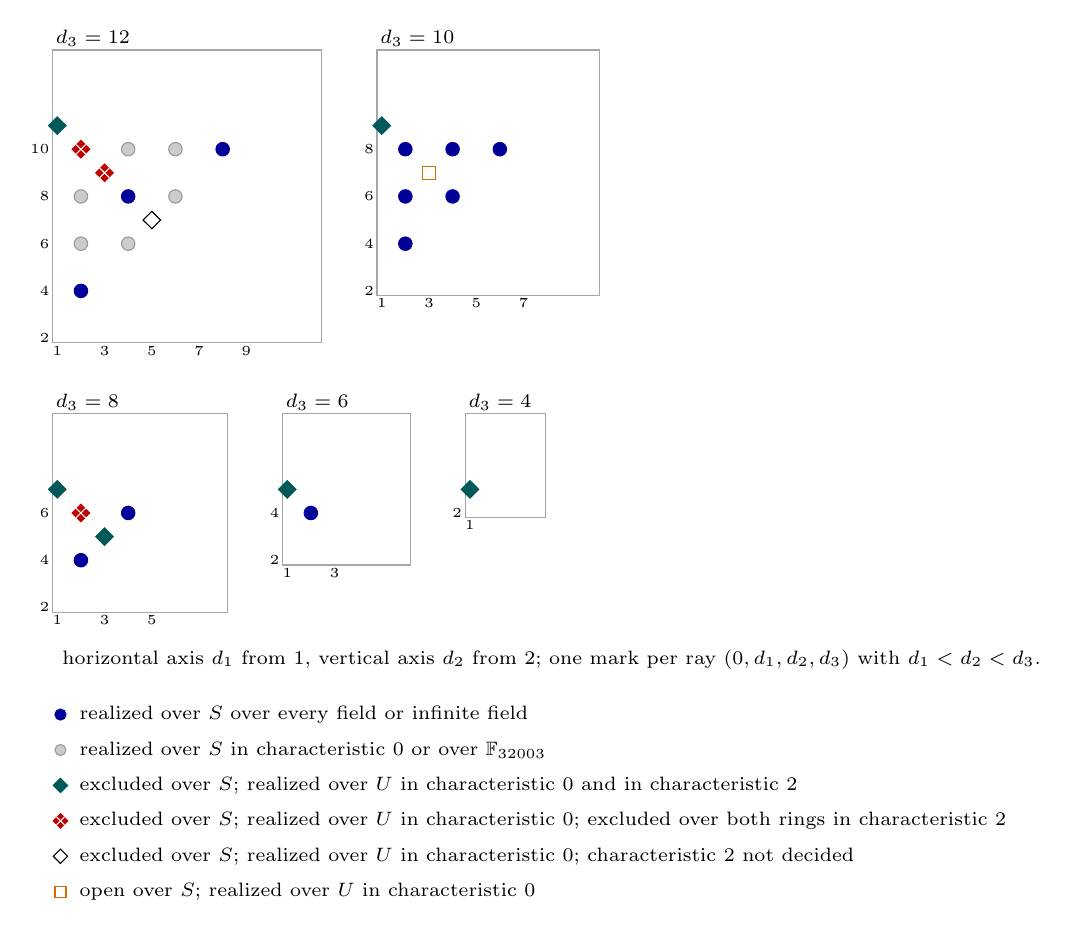
\begin{tikzpicture}[x=1cm,y=1cm,font=\scriptsize]
\begin{scope}[shift={(0.000,-3.720)}]
\draw[gray!70, line width=0.4pt] (0,0) rectangle (3.420,3.720);
\node[anchor=south west,inner sep=1pt] at (0,3.720) {$d_3=12$};
\node[anchor=north,inner sep=1pt,font=\tiny] at (0.060,0) {1};
\node[anchor=north,inner sep=1pt,font=\tiny] at (0.660,0) {3};
\node[anchor=north,inner sep=1pt,font=\tiny] at (1.260,0) {5};
\node[anchor=north,inner sep=1pt,font=\tiny] at (1.860,0) {7};
\node[anchor=north,inner sep=1pt,font=\tiny] at (2.460,0) {9};
\node[anchor=east,inner sep=1pt,font=\tiny] at (0,0.060) {2};
\node[anchor=east,inner sep=1pt,font=\tiny] at (0,0.660) {4};
\node[anchor=east,inner sep=1pt,font=\tiny] at (0,1.260) {6};
\node[anchor=east,inner sep=1pt,font=\tiny] at (0,1.860) {8};
\node[anchor=east,inner sep=1pt,font=\tiny] at (0,2.460) {10};
\draw[teal!70!black, fill=teal!70!black, line width=0.4pt] (-0.051,2.760) -- (0.060,2.870) -- (0.171,2.760) -- (0.060,2.649) -- cycle;
\draw[blue!60!black, fill=blue!60!black, line width=0.4pt] (0.360,0.660) circle (0.085);
\draw[gray!80, fill=gray!40, line width=0.4pt] (0.360,1.260) circle (0.085);
\draw[gray!80, fill=gray!40, line width=0.4pt] (0.360,1.860) circle (0.085);
\draw[red!75!black, fill=red!75!black, line width=0.4pt] (0.249,2.460) -- (0.360,2.571) -- (0.471,2.460) -- (0.360,2.349) -- cycle; \draw[white, line width=0.4pt] (0.300,2.401) -- (0.419,2.519) (0.300,2.519) -- (0.419,2.401);
\draw[red!75!black, fill=red!75!black, line width=0.4pt] (0.549,2.160) -- (0.660,2.271) -- (0.770,2.160) -- (0.660,2.050) -- cycle; \draw[white, line width=0.4pt] (0.600,2.101) -- (0.719,2.220) (0.600,2.220) -- (0.719,2.101);
\draw[gray!80, fill=gray!40, line width=0.4pt] (0.960,1.260) circle (0.085);
\draw[blue!60!black, fill=blue!60!black, line width=0.4pt] (0.960,1.860) circle (0.085);
\draw[gray!80, fill=gray!40, line width=0.4pt] (0.960,2.460) circle (0.085);
\draw[black, fill=white, line width=0.4pt] (1.149,1.560) -- (1.260,1.671) -- (1.371,1.560) -- (1.260,1.450) -- cycle;
\draw[gray!80, fill=gray!40, line width=0.4pt] (1.560,1.860) circle (0.085);
\draw[gray!80, fill=gray!40, line width=0.4pt] (1.560,2.460) circle (0.085);
\draw[blue!60!black, fill=blue!60!black, line width=0.4pt] (2.160,2.460) circle (0.085);
\end{scope}
\begin{scope}[shift={(4.120,-3.120)}]
\draw[gray!70, line width=0.4pt] (0,0) rectangle (2.820,3.120);
\node[anchor=south west,inner sep=1pt] at (0,3.120) {$d_3=10$};
\node[anchor=north,inner sep=1pt,font=\tiny] at (0.060,0) {1};
\node[anchor=north,inner sep=1pt,font=\tiny] at (0.660,0) {3};
\node[anchor=north,inner sep=1pt,font=\tiny] at (1.260,0) {5};
\node[anchor=north,inner sep=1pt,font=\tiny] at (1.860,0) {7};
\node[anchor=east,inner sep=1pt,font=\tiny] at (0,0.060) {2};
\node[anchor=east,inner sep=1pt,font=\tiny] at (0,0.660) {4};
\node[anchor=east,inner sep=1pt,font=\tiny] at (0,1.260) {6};
\node[anchor=east,inner sep=1pt,font=\tiny] at (0,1.860) {8};
\draw[teal!70!black, fill=teal!70!black, line width=0.4pt] (-0.051,2.160) -- (0.060,2.271) -- (0.171,2.160) -- (0.060,2.050) -- cycle;
\draw[blue!60!black, fill=blue!60!black, line width=0.4pt] (0.360,0.660) circle (0.085);
\draw[blue!60!black, fill=blue!60!black, line width=0.4pt] (0.360,1.260) circle (0.085);
\draw[blue!60!black, fill=blue!60!black, line width=0.4pt] (0.360,1.860) circle (0.085);
\draw[orange!85!black, fill=white, line width=0.4pt] (0.575,1.475) rectangle (0.745,1.645);
\draw[blue!60!black, fill=blue!60!black, line width=0.4pt] (0.960,1.260) circle (0.085);
\draw[blue!60!black, fill=blue!60!black, line width=0.4pt] (0.960,1.860) circle (0.085);
\draw[blue!60!black, fill=blue!60!black, line width=0.4pt] (1.560,1.860) circle (0.085);
\end{scope}
\begin{scope}[shift={(0.000,-7.140)}]
\draw[gray!70, line width=0.4pt] (0,0) rectangle (2.220,2.520);
\node[anchor=south west,inner sep=1pt] at (0,2.520) {$d_3=8$};
\node[anchor=north,inner sep=1pt,font=\tiny] at (0.060,0) {1};
\node[anchor=north,inner sep=1pt,font=\tiny] at (0.660,0) {3};
\node[anchor=north,inner sep=1pt,font=\tiny] at (1.260,0) {5};
\node[anchor=east,inner sep=1pt,font=\tiny] at (0,0.060) {2};
\node[anchor=east,inner sep=1pt,font=\tiny] at (0,0.660) {4};
\node[anchor=east,inner sep=1pt,font=\tiny] at (0,1.260) {6};
\draw[teal!70!black, fill=teal!70!black, line width=0.4pt] (-0.051,1.560) -- (0.060,1.671) -- (0.171,1.560) -- (0.060,1.450) -- cycle;
\draw[blue!60!black, fill=blue!60!black, line width=0.4pt] (0.360,0.660) circle (0.085);
\draw[red!75!black, fill=red!75!black, line width=0.4pt] (0.249,1.260) -- (0.360,1.371) -- (0.471,1.260) -- (0.360,1.149) -- cycle; \draw[white, line width=0.4pt] (0.300,1.200) -- (0.419,1.320) (0.300,1.320) -- (0.419,1.200);
\draw[teal!70!black, fill=teal!70!black, line width=0.4pt] (0.549,0.960) -- (0.660,1.071) -- (0.770,0.960) -- (0.660,0.849) -- cycle;
\draw[blue!60!black, fill=blue!60!black, line width=0.4pt] (0.960,1.260) circle (0.085);
\end{scope}
\begin{scope}[shift={(2.920,-6.540)}]
\draw[gray!70, line width=0.4pt] (0,0) rectangle (1.620,1.920);
\node[anchor=south west,inner sep=1pt] at (0,1.920) {$d_3=6$};
\node[anchor=north,inner sep=1pt,font=\tiny] at (0.060,0) {1};
\node[anchor=north,inner sep=1pt,font=\tiny] at (0.660,0) {3};
\node[anchor=east,inner sep=1pt,font=\tiny] at (0,0.060) {2};
\node[anchor=east,inner sep=1pt,font=\tiny] at (0,0.660) {4};
\draw[teal!70!black, fill=teal!70!black, line width=0.4pt] (-0.051,0.960) -- (0.060,1.071) -- (0.171,0.960) -- (0.060,0.849) -- cycle;
\draw[blue!60!black, fill=blue!60!black, line width=0.4pt] (0.360,0.660) circle (0.085);
\end{scope}
\begin{scope}[shift={(5.240,-5.940)}]
\draw[gray!70, line width=0.4pt] (0,0) rectangle (1.020,1.320);
\node[anchor=south west,inner sep=1pt] at (0,1.320) {$d_3=4$};
\node[anchor=north,inner sep=1pt,font=\tiny] at (0.060,0) {1};
\node[anchor=east,inner sep=1pt,font=\tiny] at (0,0.060) {2};
\draw[teal!70!black, fill=teal!70!black, line width=0.4pt] (-0.051,0.360) -- (0.060,0.471) -- (0.171,0.360) -- (0.060,0.249) -- cycle;
\end{scope}
\node[anchor=north west,font=\scriptsize] at (0,-7.490) {horizontal axis $d_1$ from 1, vertical axis $d_2$ from 2; one mark per ray $(0,d_1,d_2,d_3)$ with $d_1<d_2<d_3$.};
\draw[blue!60!black, fill=blue!60!black, line width=0.4pt] (0.100,-8.440) circle (0.070);
\node[anchor=west,font=\scriptsize,inner sep=1pt] at (0.30,-8.44) {realized over $S$ over every field or infinite field};
\draw[gray!80, fill=gray!40, line width=0.4pt] (0.100,-8.890) circle (0.070);
\node[anchor=west,font=\scriptsize,inner sep=1pt] at (0.30,-8.89) {realized over $S$ in characteristic 0 or over $\mathbb{F}_{32003}$};
\draw[teal!70!black, fill=teal!70!black, line width=0.4pt] (0.009,-9.340) -- (0.100,-9.249) -- (0.191,-9.340) -- (0.100,-9.431) -- cycle;
\node[anchor=west,font=\scriptsize,inner sep=1pt] at (0.30,-9.34) {excluded over $S$; realized over $U$ in characteristic 0 and in characteristic 2};
\draw[red!75!black, fill=red!75!black, line width=0.4pt] (0.009,-9.790) -- (0.100,-9.699) -- (0.191,-9.790) -- (0.100,-9.881) -- cycle; \draw[white, line width=0.4pt] (0.051,-9.839) -- (0.149,-9.741) (0.051,-9.741) -- (0.149,-9.839);
\node[anchor=west,font=\scriptsize,inner sep=1pt] at (0.30,-9.79) {excluded over $S$; realized over $U$ in characteristic 0; excluded over both rings in characteristic 2};
\draw[black, fill=white, line width=0.4pt] (0.009,-10.240) -- (0.100,-10.149) -- (0.191,-10.240) -- (0.100,-10.331) -- cycle;
\node[anchor=west,font=\scriptsize,inner sep=1pt] at (0.30,-10.24) {excluded over $S$; realized over $U$ in characteristic 0; characteristic 2 not decided};
\draw[orange!85!black, fill=white, line width=0.4pt] (0.030,-10.760) rectangle (0.170,-10.620);
\node[anchor=west,font=\scriptsize,inner sep=1pt] at (0.30,-10.69) {open over $S$; realized over $U$ in characteristic 0};
\end{tikzpicture}

\caption{The $29$ rays with $d_3\le12$ that pass the parity test, in the plane $(d_1,d_2)$ with one panel per $d_3$: circles are rays realized over $S$ (filled blue over every field or infinite field, gray otherwise), diamonds are rays excluded over $S$ and realized over $U$ in characteristic $0$ (teal: also in characteristic $2$; red with a cross: excluded over both rings in characteristic $2$ by Theorem~C; white: characteristic $2$ not decided), and the square is the ray $(0,3,7,10)$, open over $S$ and realized over $U$.}
\label{fig:lattice-u}
\end{figure}

\subsection{The census over \texorpdfstring{$S$}{S}}

\begin{table}[htbp]
\centering\footnotesize
\begin{tabular}{@{}lrrrrrr@{}}
\toprule
After & realized & every field & char.\ 0 & excluded & open & $c_d$ known\\
\midrule
formulas and closures & 78 & 52 & 78 & 12 & 130 & 86\\
known-answer runs & 88 & 52 & 78 & 12 & 120 & 98\\
level-module family & 88 & 52 & 78 & 12 & 120 & 98\\
search & 193 & 52 & 78 & 12 & 15 & 205\\
rational rechecks & 193 & 52 & 147 & 12 & 15 & 205\\
\bottomrule
\end{tabular}

\caption{The census of the \nrays{} rays with $d_3\le12$ after each stage: number of rays whose primitive point is realized in some field, realized over every field or every infinite field, realized in characteristic $0$, excluded, open, and number of rays on which the least multiple $c_d$ is known; the stage with the rank certificates gives the final table.}
\label{tab:stage}
\end{table}

Table~\ref{tab:stage} and Figure~\ref{fig:stages} give the census after each stage. The formulas and closures realize \nstageZeroRealized{} primitive points, of which \nstageZeroEvery{} over every field or every infinite field and \nstageZeroWeyman{} in characteristic $0$ by the second Eisenbud--Fl{\o}ystad--Weyman formula, and exclude $12$; the \nstageZeroOpen{} rays left open go to the search. The level-module family of S\"oderberg is pure on \nsoderbergPure{} of \nsoderbergRays{} rays at the predicted multiple. The search over $\F_{32003}$ ran \ncellsMain{} cells (\nhitsMain{} hits) and the characteristic flags \ncellsOneE{} cells (\nhitsFlag{} hits, \ncellsErr{} errors), with no timeouts, and leaves \nopen{} rays open; the final table has the primitive point realized on \nrealized{} rays, of which \nrealizedZero{} in characteristic $0$ by a cited construction or a resolution over $\Q$ (\nrealizedEvery{} over every field or every infinite field, \nrealizedZeroOnly{} in characteristic $0$ only) and the other \nrealizedPrimeOnly{} by a hit over $\F_{32003}$, all with $d_3\ge10$, which the rank certificate carries to characteristic $0$ (Section~\ref{sec:lift-results}); the least multiple is $1$ on \nrealized{} rays and $2$ on the \nexcluded{} excluded rays, and is therefore known in characteristic $0$ on \ncDetermined{} rays (with Proposition~\ref{prop:lift} for the rays realized over $\F_{32003}$ by a hit). Figure~\ref{fig:lattice-s} shows the status of every ray.

\begin{figure}[htbp]
\centering
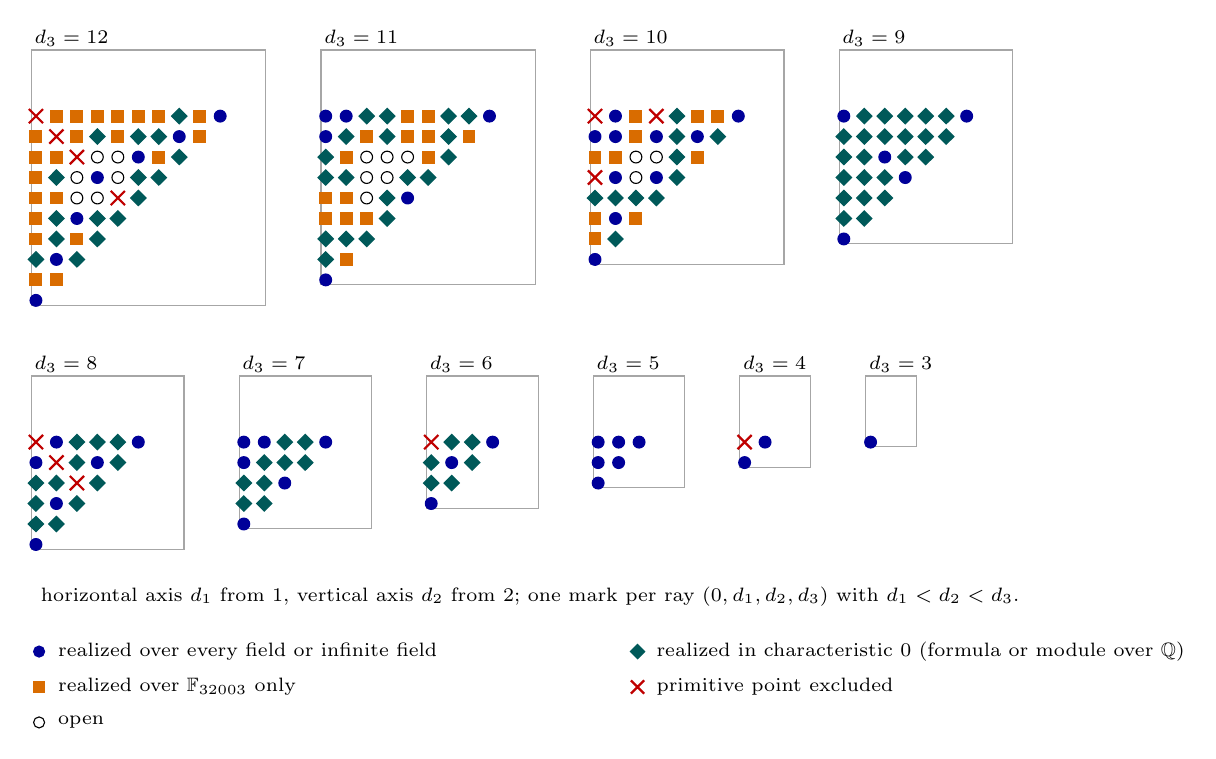
\begin{tikzpicture}[x=1cm,y=1cm,font=\scriptsize]
\begin{scope}[shift={(0.000,-3.240)}]
\draw[gray!70, line width=0.4pt] (0,0) rectangle (2.980,3.240);
\node[anchor=south west,inner sep=1pt] at (0,3.240) {$d_3=12$};
\draw[blue!60!black, fill=blue!60!black, line width=0.4pt] (0.060,0.060) circle (0.075);
\draw[orange!85!black, fill=orange!85!black, line width=0.4pt] (-0.015,0.245) rectangle (0.135,0.395);
\draw[teal!70!black, fill=teal!70!black, line width=0.4pt] (-0.038,0.580) -- (0.060,0.678) -- (0.158,0.580) -- (0.060,0.483) -- cycle;
\draw[orange!85!black, fill=orange!85!black, line width=0.4pt] (-0.015,0.765) rectangle (0.135,0.915);
\draw[orange!85!black, fill=orange!85!black, line width=0.4pt] (-0.015,1.025) rectangle (0.135,1.175);
\draw[orange!85!black, fill=orange!85!black, line width=0.4pt] (-0.015,1.285) rectangle (0.135,1.435);
\draw[orange!85!black, fill=orange!85!black, line width=0.4pt] (-0.015,1.545) rectangle (0.135,1.695);
\draw[orange!85!black, fill=orange!85!black, line width=0.4pt] (-0.015,1.805) rectangle (0.135,1.955);
\draw[orange!85!black, fill=orange!85!black, line width=0.4pt] (-0.015,2.065) rectangle (0.135,2.215);
\draw[red!75!black, line width=0.8pt] (-0.030,2.310) -- (0.150,2.490) (-0.030,2.490) -- (0.150,2.310);
\draw[orange!85!black, fill=orange!85!black, line width=0.4pt] (0.245,0.245) rectangle (0.395,0.395);
\draw[blue!60!black, fill=blue!60!black, line width=0.4pt] (0.320,0.580) circle (0.075);
\draw[teal!70!black, fill=teal!70!black, line width=0.4pt] (0.223,0.840) -- (0.320,0.938) -- (0.417,0.840) -- (0.320,0.743) -- cycle;
\draw[teal!70!black, fill=teal!70!black, line width=0.4pt] (0.223,1.100) -- (0.320,1.198) -- (0.417,1.100) -- (0.320,1.003) -- cycle;
\draw[orange!85!black, fill=orange!85!black, line width=0.4pt] (0.245,1.285) rectangle (0.395,1.435);
\draw[teal!70!black, fill=teal!70!black, line width=0.4pt] (0.223,1.620) -- (0.320,1.718) -- (0.417,1.620) -- (0.320,1.523) -- cycle;
\draw[orange!85!black, fill=orange!85!black, line width=0.4pt] (0.245,1.805) rectangle (0.395,1.955);
\draw[red!75!black, line width=0.8pt] (0.230,2.050) -- (0.410,2.230) (0.230,2.230) -- (0.410,2.050);
\draw[orange!85!black, fill=orange!85!black, line width=0.4pt] (0.245,2.325) rectangle (0.395,2.475);
\draw[teal!70!black, fill=teal!70!black, line width=0.4pt] (0.483,0.580) -- (0.580,0.678) -- (0.678,0.580) -- (0.580,0.483) -- cycle;
\draw[orange!85!black, fill=orange!85!black, line width=0.4pt] (0.505,0.765) rectangle (0.655,0.915);
\draw[blue!60!black, fill=blue!60!black, line width=0.4pt] (0.580,1.100) circle (0.075);
\draw[black, fill=white, line width=0.4pt] (0.580,1.360) circle (0.075);
\draw[black, fill=white, line width=0.4pt] (0.580,1.620) circle (0.075);
\draw[red!75!black, line width=0.8pt] (0.490,1.790) -- (0.670,1.970) (0.490,1.970) -- (0.670,1.790);
\draw[orange!85!black, fill=orange!85!black, line width=0.4pt] (0.505,2.065) rectangle (0.655,2.215);
\draw[orange!85!black, fill=orange!85!black, line width=0.4pt] (0.505,2.325) rectangle (0.655,2.475);
\draw[teal!70!black, fill=teal!70!black, line width=0.4pt] (0.743,0.840) -- (0.840,0.938) -- (0.938,0.840) -- (0.840,0.743) -- cycle;
\draw[teal!70!black, fill=teal!70!black, line width=0.4pt] (0.743,1.100) -- (0.840,1.198) -- (0.938,1.100) -- (0.840,1.003) -- cycle;
\draw[black, fill=white, line width=0.4pt] (0.840,1.360) circle (0.075);
\draw[blue!60!black, fill=blue!60!black, line width=0.4pt] (0.840,1.620) circle (0.075);
\draw[black, fill=white, line width=0.4pt] (0.840,1.880) circle (0.075);
\draw[teal!70!black, fill=teal!70!black, line width=0.4pt] (0.743,2.140) -- (0.840,2.238) -- (0.938,2.140) -- (0.840,2.042) -- cycle;
\draw[orange!85!black, fill=orange!85!black, line width=0.4pt] (0.765,2.325) rectangle (0.915,2.475);
\draw[teal!70!black, fill=teal!70!black, line width=0.4pt] (1.003,1.100) -- (1.100,1.198) -- (1.198,1.100) -- (1.100,1.003) -- cycle;
\draw[red!75!black, line width=0.8pt] (1.010,1.270) -- (1.190,1.450) (1.010,1.450) -- (1.190,1.270);
\draw[black, fill=white, line width=0.4pt] (1.100,1.620) circle (0.075);
\draw[black, fill=white, line width=0.4pt] (1.100,1.880) circle (0.075);
\draw[orange!85!black, fill=orange!85!black, line width=0.4pt] (1.025,2.065) rectangle (1.175,2.215);
\draw[orange!85!black, fill=orange!85!black, line width=0.4pt] (1.025,2.325) rectangle (1.175,2.475);
\draw[teal!70!black, fill=teal!70!black, line width=0.4pt] (1.263,1.360) -- (1.360,1.458) -- (1.458,1.360) -- (1.360,1.263) -- cycle;
\draw[teal!70!black, fill=teal!70!black, line width=0.4pt] (1.263,1.620) -- (1.360,1.718) -- (1.458,1.620) -- (1.360,1.523) -- cycle;
\draw[blue!60!black, fill=blue!60!black, line width=0.4pt] (1.360,1.880) circle (0.075);
\draw[teal!70!black, fill=teal!70!black, line width=0.4pt] (1.263,2.140) -- (1.360,2.238) -- (1.458,2.140) -- (1.360,2.042) -- cycle;
\draw[orange!85!black, fill=orange!85!black, line width=0.4pt] (1.285,2.325) rectangle (1.435,2.475);
\draw[teal!70!black, fill=teal!70!black, line width=0.4pt] (1.523,1.620) -- (1.620,1.718) -- (1.718,1.620) -- (1.620,1.523) -- cycle;
\draw[orange!85!black, fill=orange!85!black, line width=0.4pt] (1.545,1.805) rectangle (1.695,1.955);
\draw[teal!70!black, fill=teal!70!black, line width=0.4pt] (1.523,2.140) -- (1.620,2.238) -- (1.718,2.140) -- (1.620,2.042) -- cycle;
\draw[orange!85!black, fill=orange!85!black, line width=0.4pt] (1.545,2.325) rectangle (1.695,2.475);
\draw[teal!70!black, fill=teal!70!black, line width=0.4pt] (1.783,1.880) -- (1.880,1.978) -- (1.978,1.880) -- (1.880,1.783) -- cycle;
\draw[blue!60!black, fill=blue!60!black, line width=0.4pt] (1.880,2.140) circle (0.075);
\draw[teal!70!black, fill=teal!70!black, line width=0.4pt] (1.783,2.400) -- (1.880,2.498) -- (1.978,2.400) -- (1.880,2.302) -- cycle;
\draw[orange!85!black, fill=orange!85!black, line width=0.4pt] (2.065,2.065) rectangle (2.215,2.215);
\draw[orange!85!black, fill=orange!85!black, line width=0.4pt] (2.065,2.325) rectangle (2.215,2.475);
\draw[blue!60!black, fill=blue!60!black, line width=0.4pt] (2.400,2.400) circle (0.075);
\end{scope}
\begin{scope}[shift={(3.680,-2.980)}]
\draw[gray!70, line width=0.4pt] (0,0) rectangle (2.720,2.980);
\node[anchor=south west,inner sep=1pt] at (0,2.980) {$d_3=11$};
\draw[blue!60!black, fill=blue!60!black, line width=0.4pt] (0.060,0.060) circle (0.075);
\draw[teal!70!black, fill=teal!70!black, line width=0.4pt] (-0.038,0.320) -- (0.060,0.417) -- (0.158,0.320) -- (0.060,0.223) -- cycle;
\draw[teal!70!black, fill=teal!70!black, line width=0.4pt] (-0.038,0.580) -- (0.060,0.678) -- (0.158,0.580) -- (0.060,0.483) -- cycle;
\draw[orange!85!black, fill=orange!85!black, line width=0.4pt] (-0.015,0.765) rectangle (0.135,0.915);
\draw[orange!85!black, fill=orange!85!black, line width=0.4pt] (-0.015,1.025) rectangle (0.135,1.175);
\draw[teal!70!black, fill=teal!70!black, line width=0.4pt] (-0.038,1.360) -- (0.060,1.458) -- (0.158,1.360) -- (0.060,1.263) -- cycle;
\draw[teal!70!black, fill=teal!70!black, line width=0.4pt] (-0.038,1.620) -- (0.060,1.718) -- (0.158,1.620) -- (0.060,1.523) -- cycle;
\draw[blue!60!black, fill=blue!60!black, line width=0.4pt] (0.060,1.880) circle (0.075);
\draw[blue!60!black, fill=blue!60!black, line width=0.4pt] (0.060,2.140) circle (0.075);
\draw[orange!85!black, fill=orange!85!black, line width=0.4pt] (0.245,0.245) rectangle (0.395,0.395);
\draw[teal!70!black, fill=teal!70!black, line width=0.4pt] (0.223,0.580) -- (0.320,0.678) -- (0.417,0.580) -- (0.320,0.483) -- cycle;
\draw[orange!85!black, fill=orange!85!black, line width=0.4pt] (0.245,0.765) rectangle (0.395,0.915);
\draw[orange!85!black, fill=orange!85!black, line width=0.4pt] (0.245,1.025) rectangle (0.395,1.175);
\draw[teal!70!black, fill=teal!70!black, line width=0.4pt] (0.223,1.360) -- (0.320,1.458) -- (0.417,1.360) -- (0.320,1.263) -- cycle;
\draw[orange!85!black, fill=orange!85!black, line width=0.4pt] (0.245,1.545) rectangle (0.395,1.695);
\draw[teal!70!black, fill=teal!70!black, line width=0.4pt] (0.223,1.880) -- (0.320,1.978) -- (0.417,1.880) -- (0.320,1.783) -- cycle;
\draw[blue!60!black, fill=blue!60!black, line width=0.4pt] (0.320,2.140) circle (0.075);
\draw[teal!70!black, fill=teal!70!black, line width=0.4pt] (0.483,0.580) -- (0.580,0.678) -- (0.678,0.580) -- (0.580,0.483) -- cycle;
\draw[orange!85!black, fill=orange!85!black, line width=0.4pt] (0.505,0.765) rectangle (0.655,0.915);
\draw[black, fill=white, line width=0.4pt] (0.580,1.100) circle (0.075);
\draw[black, fill=white, line width=0.4pt] (0.580,1.360) circle (0.075);
\draw[black, fill=white, line width=0.4pt] (0.580,1.620) circle (0.075);
\draw[orange!85!black, fill=orange!85!black, line width=0.4pt] (0.505,1.805) rectangle (0.655,1.955);
\draw[teal!70!black, fill=teal!70!black, line width=0.4pt] (0.483,2.140) -- (0.580,2.238) -- (0.678,2.140) -- (0.580,2.042) -- cycle;
\draw[teal!70!black, fill=teal!70!black, line width=0.4pt] (0.743,0.840) -- (0.840,0.938) -- (0.938,0.840) -- (0.840,0.743) -- cycle;
\draw[teal!70!black, fill=teal!70!black, line width=0.4pt] (0.743,1.100) -- (0.840,1.198) -- (0.938,1.100) -- (0.840,1.003) -- cycle;
\draw[black, fill=white, line width=0.4pt] (0.840,1.360) circle (0.075);
\draw[black, fill=white, line width=0.4pt] (0.840,1.620) circle (0.075);
\draw[teal!70!black, fill=teal!70!black, line width=0.4pt] (0.743,1.880) -- (0.840,1.978) -- (0.938,1.880) -- (0.840,1.783) -- cycle;
\draw[teal!70!black, fill=teal!70!black, line width=0.4pt] (0.743,2.140) -- (0.840,2.238) -- (0.938,2.140) -- (0.840,2.042) -- cycle;
\draw[blue!60!black, fill=blue!60!black, line width=0.4pt] (1.100,1.100) circle (0.075);
\draw[teal!70!black, fill=teal!70!black, line width=0.4pt] (1.003,1.360) -- (1.100,1.458) -- (1.198,1.360) -- (1.100,1.263) -- cycle;
\draw[black, fill=white, line width=0.4pt] (1.100,1.620) circle (0.075);
\draw[orange!85!black, fill=orange!85!black, line width=0.4pt] (1.025,1.805) rectangle (1.175,1.955);
\draw[orange!85!black, fill=orange!85!black, line width=0.4pt] (1.025,2.065) rectangle (1.175,2.215);
\draw[teal!70!black, fill=teal!70!black, line width=0.4pt] (1.263,1.360) -- (1.360,1.458) -- (1.458,1.360) -- (1.360,1.263) -- cycle;
\draw[orange!85!black, fill=orange!85!black, line width=0.4pt] (1.285,1.545) rectangle (1.435,1.695);
\draw[orange!85!black, fill=orange!85!black, line width=0.4pt] (1.285,1.805) rectangle (1.435,1.955);
\draw[orange!85!black, fill=orange!85!black, line width=0.4pt] (1.285,2.065) rectangle (1.435,2.215);
\draw[teal!70!black, fill=teal!70!black, line width=0.4pt] (1.523,1.620) -- (1.620,1.718) -- (1.718,1.620) -- (1.620,1.523) -- cycle;
\draw[teal!70!black, fill=teal!70!black, line width=0.4pt] (1.523,1.880) -- (1.620,1.978) -- (1.718,1.880) -- (1.620,1.783) -- cycle;
\draw[teal!70!black, fill=teal!70!black, line width=0.4pt] (1.523,2.140) -- (1.620,2.238) -- (1.718,2.140) -- (1.620,2.042) -- cycle;
\draw[orange!85!black, fill=orange!85!black, line width=0.4pt] (1.805,1.805) rectangle (1.955,1.955);
\draw[teal!70!black, fill=teal!70!black, line width=0.4pt] (1.783,2.140) -- (1.880,2.238) -- (1.978,2.140) -- (1.880,2.042) -- cycle;
\draw[blue!60!black, fill=blue!60!black, line width=0.4pt] (2.140,2.140) circle (0.075);
\end{scope}
\begin{scope}[shift={(7.100,-2.720)}]
\draw[gray!70, line width=0.4pt] (0,0) rectangle (2.460,2.720);
\node[anchor=south west,inner sep=1pt] at (0,2.720) {$d_3=10$};
\draw[blue!60!black, fill=blue!60!black, line width=0.4pt] (0.060,0.060) circle (0.075);
\draw[orange!85!black, fill=orange!85!black, line width=0.4pt] (-0.015,0.245) rectangle (0.135,0.395);
\draw[orange!85!black, fill=orange!85!black, line width=0.4pt] (-0.015,0.505) rectangle (0.135,0.655);
\draw[teal!70!black, fill=teal!70!black, line width=0.4pt] (-0.038,0.840) -- (0.060,0.938) -- (0.158,0.840) -- (0.060,0.743) -- cycle;
\draw[red!75!black, line width=0.8pt] (-0.030,1.010) -- (0.150,1.190) (-0.030,1.190) -- (0.150,1.010);
\draw[orange!85!black, fill=orange!85!black, line width=0.4pt] (-0.015,1.285) rectangle (0.135,1.435);
\draw[blue!60!black, fill=blue!60!black, line width=0.4pt] (0.060,1.620) circle (0.075);
\draw[red!75!black, line width=0.8pt] (-0.030,1.790) -- (0.150,1.970) (-0.030,1.970) -- (0.150,1.790);
\draw[teal!70!black, fill=teal!70!black, line width=0.4pt] (0.223,0.320) -- (0.320,0.417) -- (0.417,0.320) -- (0.320,0.223) -- cycle;
\draw[blue!60!black, fill=blue!60!black, line width=0.4pt] (0.320,0.580) circle (0.075);
\draw[teal!70!black, fill=teal!70!black, line width=0.4pt] (0.223,0.840) -- (0.320,0.938) -- (0.417,0.840) -- (0.320,0.743) -- cycle;
\draw[blue!60!black, fill=blue!60!black, line width=0.4pt] (0.320,1.100) circle (0.075);
\draw[orange!85!black, fill=orange!85!black, line width=0.4pt] (0.245,1.285) rectangle (0.395,1.435);
\draw[blue!60!black, fill=blue!60!black, line width=0.4pt] (0.320,1.620) circle (0.075);
\draw[blue!60!black, fill=blue!60!black, line width=0.4pt] (0.320,1.880) circle (0.075);
\draw[orange!85!black, fill=orange!85!black, line width=0.4pt] (0.505,0.505) rectangle (0.655,0.655);
\draw[teal!70!black, fill=teal!70!black, line width=0.4pt] (0.483,0.840) -- (0.580,0.938) -- (0.678,0.840) -- (0.580,0.743) -- cycle;
\draw[black, fill=white, line width=0.4pt] (0.580,1.100) circle (0.075);
\draw[black, fill=white, line width=0.4pt] (0.580,1.360) circle (0.075);
\draw[orange!85!black, fill=orange!85!black, line width=0.4pt] (0.505,1.545) rectangle (0.655,1.695);
\draw[orange!85!black, fill=orange!85!black, line width=0.4pt] (0.505,1.805) rectangle (0.655,1.955);
\draw[teal!70!black, fill=teal!70!black, line width=0.4pt] (0.743,0.840) -- (0.840,0.938) -- (0.938,0.840) -- (0.840,0.743) -- cycle;
\draw[blue!60!black, fill=blue!60!black, line width=0.4pt] (0.840,1.100) circle (0.075);
\draw[black, fill=white, line width=0.4pt] (0.840,1.360) circle (0.075);
\draw[blue!60!black, fill=blue!60!black, line width=0.4pt] (0.840,1.620) circle (0.075);
\draw[red!75!black, line width=0.8pt] (0.750,1.790) -- (0.930,1.970) (0.750,1.970) -- (0.930,1.790);
\draw[teal!70!black, fill=teal!70!black, line width=0.4pt] (1.003,1.100) -- (1.100,1.198) -- (1.198,1.100) -- (1.100,1.003) -- cycle;
\draw[teal!70!black, fill=teal!70!black, line width=0.4pt] (1.003,1.360) -- (1.100,1.458) -- (1.198,1.360) -- (1.100,1.263) -- cycle;
\draw[teal!70!black, fill=teal!70!black, line width=0.4pt] (1.003,1.620) -- (1.100,1.718) -- (1.198,1.620) -- (1.100,1.523) -- cycle;
\draw[teal!70!black, fill=teal!70!black, line width=0.4pt] (1.003,1.880) -- (1.100,1.978) -- (1.198,1.880) -- (1.100,1.783) -- cycle;
\draw[orange!85!black, fill=orange!85!black, line width=0.4pt] (1.285,1.285) rectangle (1.435,1.435);
\draw[blue!60!black, fill=blue!60!black, line width=0.4pt] (1.360,1.620) circle (0.075);
\draw[orange!85!black, fill=orange!85!black, line width=0.4pt] (1.285,1.805) rectangle (1.435,1.955);
\draw[teal!70!black, fill=teal!70!black, line width=0.4pt] (1.523,1.620) -- (1.620,1.718) -- (1.718,1.620) -- (1.620,1.523) -- cycle;
\draw[orange!85!black, fill=orange!85!black, line width=0.4pt] (1.545,1.805) rectangle (1.695,1.955);
\draw[blue!60!black, fill=blue!60!black, line width=0.4pt] (1.880,1.880) circle (0.075);
\end{scope}
\begin{scope}[shift={(10.260,-2.460)}]
\draw[gray!70, line width=0.4pt] (0,0) rectangle (2.200,2.460);
\node[anchor=south west,inner sep=1pt] at (0,2.460) {$d_3=9$};
\draw[blue!60!black, fill=blue!60!black, line width=0.4pt] (0.060,0.060) circle (0.075);
\draw[teal!70!black, fill=teal!70!black, line width=0.4pt] (-0.038,0.320) -- (0.060,0.417) -- (0.158,0.320) -- (0.060,0.223) -- cycle;
\draw[teal!70!black, fill=teal!70!black, line width=0.4pt] (-0.038,0.580) -- (0.060,0.678) -- (0.158,0.580) -- (0.060,0.483) -- cycle;
\draw[teal!70!black, fill=teal!70!black, line width=0.4pt] (-0.038,0.840) -- (0.060,0.938) -- (0.158,0.840) -- (0.060,0.743) -- cycle;
\draw[teal!70!black, fill=teal!70!black, line width=0.4pt] (-0.038,1.100) -- (0.060,1.198) -- (0.158,1.100) -- (0.060,1.003) -- cycle;
\draw[teal!70!black, fill=teal!70!black, line width=0.4pt] (-0.038,1.360) -- (0.060,1.458) -- (0.158,1.360) -- (0.060,1.263) -- cycle;
\draw[blue!60!black, fill=blue!60!black, line width=0.4pt] (0.060,1.620) circle (0.075);
\draw[teal!70!black, fill=teal!70!black, line width=0.4pt] (0.223,0.320) -- (0.320,0.417) -- (0.417,0.320) -- (0.320,0.223) -- cycle;
\draw[teal!70!black, fill=teal!70!black, line width=0.4pt] (0.223,0.580) -- (0.320,0.678) -- (0.417,0.580) -- (0.320,0.483) -- cycle;
\draw[teal!70!black, fill=teal!70!black, line width=0.4pt] (0.223,0.840) -- (0.320,0.938) -- (0.417,0.840) -- (0.320,0.743) -- cycle;
\draw[teal!70!black, fill=teal!70!black, line width=0.4pt] (0.223,1.100) -- (0.320,1.198) -- (0.417,1.100) -- (0.320,1.003) -- cycle;
\draw[teal!70!black, fill=teal!70!black, line width=0.4pt] (0.223,1.360) -- (0.320,1.458) -- (0.417,1.360) -- (0.320,1.263) -- cycle;
\draw[teal!70!black, fill=teal!70!black, line width=0.4pt] (0.223,1.620) -- (0.320,1.718) -- (0.417,1.620) -- (0.320,1.523) -- cycle;
\draw[teal!70!black, fill=teal!70!black, line width=0.4pt] (0.483,0.580) -- (0.580,0.678) -- (0.678,0.580) -- (0.580,0.483) -- cycle;
\draw[teal!70!black, fill=teal!70!black, line width=0.4pt] (0.483,0.840) -- (0.580,0.938) -- (0.678,0.840) -- (0.580,0.743) -- cycle;
\draw[blue!60!black, fill=blue!60!black, line width=0.4pt] (0.580,1.100) circle (0.075);
\draw[teal!70!black, fill=teal!70!black, line width=0.4pt] (0.483,1.360) -- (0.580,1.458) -- (0.678,1.360) -- (0.580,1.263) -- cycle;
\draw[teal!70!black, fill=teal!70!black, line width=0.4pt] (0.483,1.620) -- (0.580,1.718) -- (0.678,1.620) -- (0.580,1.523) -- cycle;
\draw[blue!60!black, fill=blue!60!black, line width=0.4pt] (0.840,0.840) circle (0.075);
\draw[teal!70!black, fill=teal!70!black, line width=0.4pt] (0.743,1.100) -- (0.840,1.198) -- (0.938,1.100) -- (0.840,1.003) -- cycle;
\draw[teal!70!black, fill=teal!70!black, line width=0.4pt] (0.743,1.360) -- (0.840,1.458) -- (0.938,1.360) -- (0.840,1.263) -- cycle;
\draw[teal!70!black, fill=teal!70!black, line width=0.4pt] (0.743,1.620) -- (0.840,1.718) -- (0.938,1.620) -- (0.840,1.523) -- cycle;
\draw[teal!70!black, fill=teal!70!black, line width=0.4pt] (1.003,1.100) -- (1.100,1.198) -- (1.198,1.100) -- (1.100,1.003) -- cycle;
\draw[teal!70!black, fill=teal!70!black, line width=0.4pt] (1.003,1.360) -- (1.100,1.458) -- (1.198,1.360) -- (1.100,1.263) -- cycle;
\draw[teal!70!black, fill=teal!70!black, line width=0.4pt] (1.003,1.620) -- (1.100,1.718) -- (1.198,1.620) -- (1.100,1.523) -- cycle;
\draw[teal!70!black, fill=teal!70!black, line width=0.4pt] (1.263,1.360) -- (1.360,1.458) -- (1.458,1.360) -- (1.360,1.263) -- cycle;
\draw[teal!70!black, fill=teal!70!black, line width=0.4pt] (1.263,1.620) -- (1.360,1.718) -- (1.458,1.620) -- (1.360,1.523) -- cycle;
\draw[blue!60!black, fill=blue!60!black, line width=0.4pt] (1.620,1.620) circle (0.075);
\end{scope}
\begin{scope}[shift={(0.000,-6.340)}]
\draw[gray!70, line width=0.4pt] (0,0) rectangle (1.940,2.200);
\node[anchor=south west,inner sep=1pt] at (0,2.200) {$d_3=8$};
\draw[blue!60!black, fill=blue!60!black, line width=0.4pt] (0.060,0.060) circle (0.075);
\draw[teal!70!black, fill=teal!70!black, line width=0.4pt] (-0.038,0.320) -- (0.060,0.417) -- (0.158,0.320) -- (0.060,0.223) -- cycle;
\draw[teal!70!black, fill=teal!70!black, line width=0.4pt] (-0.038,0.580) -- (0.060,0.678) -- (0.158,0.580) -- (0.060,0.483) -- cycle;
\draw[teal!70!black, fill=teal!70!black, line width=0.4pt] (-0.038,0.840) -- (0.060,0.938) -- (0.158,0.840) -- (0.060,0.743) -- cycle;
\draw[blue!60!black, fill=blue!60!black, line width=0.4pt] (0.060,1.100) circle (0.075);
\draw[red!75!black, line width=0.8pt] (-0.030,1.270) -- (0.150,1.450) (-0.030,1.450) -- (0.150,1.270);
\draw[teal!70!black, fill=teal!70!black, line width=0.4pt] (0.223,0.320) -- (0.320,0.417) -- (0.417,0.320) -- (0.320,0.223) -- cycle;
\draw[blue!60!black, fill=blue!60!black, line width=0.4pt] (0.320,0.580) circle (0.075);
\draw[teal!70!black, fill=teal!70!black, line width=0.4pt] (0.223,0.840) -- (0.320,0.938) -- (0.417,0.840) -- (0.320,0.743) -- cycle;
\draw[red!75!black, line width=0.8pt] (0.230,1.010) -- (0.410,1.190) (0.230,1.190) -- (0.410,1.010);
\draw[blue!60!black, fill=blue!60!black, line width=0.4pt] (0.320,1.360) circle (0.075);
\draw[teal!70!black, fill=teal!70!black, line width=0.4pt] (0.483,0.580) -- (0.580,0.678) -- (0.678,0.580) -- (0.580,0.483) -- cycle;
\draw[red!75!black, line width=0.8pt] (0.490,0.750) -- (0.670,0.930) (0.490,0.930) -- (0.670,0.750);
\draw[teal!70!black, fill=teal!70!black, line width=0.4pt] (0.483,1.100) -- (0.580,1.198) -- (0.678,1.100) -- (0.580,1.003) -- cycle;
\draw[teal!70!black, fill=teal!70!black, line width=0.4pt] (0.483,1.360) -- (0.580,1.458) -- (0.678,1.360) -- (0.580,1.263) -- cycle;
\draw[teal!70!black, fill=teal!70!black, line width=0.4pt] (0.743,0.840) -- (0.840,0.938) -- (0.938,0.840) -- (0.840,0.743) -- cycle;
\draw[blue!60!black, fill=blue!60!black, line width=0.4pt] (0.840,1.100) circle (0.075);
\draw[teal!70!black, fill=teal!70!black, line width=0.4pt] (0.743,1.360) -- (0.840,1.458) -- (0.938,1.360) -- (0.840,1.263) -- cycle;
\draw[teal!70!black, fill=teal!70!black, line width=0.4pt] (1.003,1.100) -- (1.100,1.198) -- (1.198,1.100) -- (1.100,1.003) -- cycle;
\draw[teal!70!black, fill=teal!70!black, line width=0.4pt] (1.003,1.360) -- (1.100,1.458) -- (1.198,1.360) -- (1.100,1.263) -- cycle;
\draw[blue!60!black, fill=blue!60!black, line width=0.4pt] (1.360,1.360) circle (0.075);
\end{scope}
\begin{scope}[shift={(2.640,-6.080)}]
\draw[gray!70, line width=0.4pt] (0,0) rectangle (1.680,1.940);
\node[anchor=south west,inner sep=1pt] at (0,1.940) {$d_3=7$};
\draw[blue!60!black, fill=blue!60!black, line width=0.4pt] (0.060,0.060) circle (0.075);
\draw[teal!70!black, fill=teal!70!black, line width=0.4pt] (-0.038,0.320) -- (0.060,0.417) -- (0.158,0.320) -- (0.060,0.223) -- cycle;
\draw[teal!70!black, fill=teal!70!black, line width=0.4pt] (-0.038,0.580) -- (0.060,0.678) -- (0.158,0.580) -- (0.060,0.483) -- cycle;
\draw[blue!60!black, fill=blue!60!black, line width=0.4pt] (0.060,0.840) circle (0.075);
\draw[blue!60!black, fill=blue!60!black, line width=0.4pt] (0.060,1.100) circle (0.075);
\draw[teal!70!black, fill=teal!70!black, line width=0.4pt] (0.223,0.320) -- (0.320,0.417) -- (0.417,0.320) -- (0.320,0.223) -- cycle;
\draw[teal!70!black, fill=teal!70!black, line width=0.4pt] (0.223,0.580) -- (0.320,0.678) -- (0.417,0.580) -- (0.320,0.483) -- cycle;
\draw[teal!70!black, fill=teal!70!black, line width=0.4pt] (0.223,0.840) -- (0.320,0.938) -- (0.417,0.840) -- (0.320,0.743) -- cycle;
\draw[blue!60!black, fill=blue!60!black, line width=0.4pt] (0.320,1.100) circle (0.075);
\draw[blue!60!black, fill=blue!60!black, line width=0.4pt] (0.580,0.580) circle (0.075);
\draw[teal!70!black, fill=teal!70!black, line width=0.4pt] (0.483,0.840) -- (0.580,0.938) -- (0.678,0.840) -- (0.580,0.743) -- cycle;
\draw[teal!70!black, fill=teal!70!black, line width=0.4pt] (0.483,1.100) -- (0.580,1.198) -- (0.678,1.100) -- (0.580,1.003) -- cycle;
\draw[teal!70!black, fill=teal!70!black, line width=0.4pt] (0.743,0.840) -- (0.840,0.938) -- (0.938,0.840) -- (0.840,0.743) -- cycle;
\draw[teal!70!black, fill=teal!70!black, line width=0.4pt] (0.743,1.100) -- (0.840,1.198) -- (0.938,1.100) -- (0.840,1.003) -- cycle;
\draw[blue!60!black, fill=blue!60!black, line width=0.4pt] (1.100,1.100) circle (0.075);
\end{scope}
\begin{scope}[shift={(5.020,-5.820)}]
\draw[gray!70, line width=0.4pt] (0,0) rectangle (1.420,1.680);
\node[anchor=south west,inner sep=1pt] at (0,1.680) {$d_3=6$};
\draw[blue!60!black, fill=blue!60!black, line width=0.4pt] (0.060,0.060) circle (0.075);
\draw[teal!70!black, fill=teal!70!black, line width=0.4pt] (-0.038,0.320) -- (0.060,0.417) -- (0.158,0.320) -- (0.060,0.223) -- cycle;
\draw[teal!70!black, fill=teal!70!black, line width=0.4pt] (-0.038,0.580) -- (0.060,0.678) -- (0.158,0.580) -- (0.060,0.483) -- cycle;
\draw[red!75!black, line width=0.8pt] (-0.030,0.750) -- (0.150,0.930) (-0.030,0.930) -- (0.150,0.750);
\draw[teal!70!black, fill=teal!70!black, line width=0.4pt] (0.223,0.320) -- (0.320,0.417) -- (0.417,0.320) -- (0.320,0.223) -- cycle;
\draw[blue!60!black, fill=blue!60!black, line width=0.4pt] (0.320,0.580) circle (0.075);
\draw[teal!70!black, fill=teal!70!black, line width=0.4pt] (0.223,0.840) -- (0.320,0.938) -- (0.417,0.840) -- (0.320,0.743) -- cycle;
\draw[teal!70!black, fill=teal!70!black, line width=0.4pt] (0.483,0.580) -- (0.580,0.678) -- (0.678,0.580) -- (0.580,0.483) -- cycle;
\draw[teal!70!black, fill=teal!70!black, line width=0.4pt] (0.483,0.840) -- (0.580,0.938) -- (0.678,0.840) -- (0.580,0.743) -- cycle;
\draw[blue!60!black, fill=blue!60!black, line width=0.4pt] (0.840,0.840) circle (0.075);
\end{scope}
\begin{scope}[shift={(7.140,-5.560)}]
\draw[gray!70, line width=0.4pt] (0,0) rectangle (1.160,1.420);
\node[anchor=south west,inner sep=1pt] at (0,1.420) {$d_3=5$};
\draw[blue!60!black, fill=blue!60!black, line width=0.4pt] (0.060,0.060) circle (0.075);
\draw[blue!60!black, fill=blue!60!black, line width=0.4pt] (0.060,0.320) circle (0.075);
\draw[blue!60!black, fill=blue!60!black, line width=0.4pt] (0.060,0.580) circle (0.075);
\draw[blue!60!black, fill=blue!60!black, line width=0.4pt] (0.320,0.320) circle (0.075);
\draw[blue!60!black, fill=blue!60!black, line width=0.4pt] (0.320,0.580) circle (0.075);
\draw[blue!60!black, fill=blue!60!black, line width=0.4pt] (0.580,0.580) circle (0.075);
\end{scope}
\begin{scope}[shift={(9.000,-5.300)}]
\draw[gray!70, line width=0.4pt] (0,0) rectangle (0.900,1.160);
\node[anchor=south west,inner sep=1pt] at (0,1.160) {$d_3=4$};
\draw[blue!60!black, fill=blue!60!black, line width=0.4pt] (0.060,0.060) circle (0.075);
\draw[red!75!black, line width=0.8pt] (-0.030,0.230) -- (0.150,0.410) (-0.030,0.410) -- (0.150,0.230);
\draw[blue!60!black, fill=blue!60!black, line width=0.4pt] (0.320,0.320) circle (0.075);
\end{scope}
\begin{scope}[shift={(10.600,-5.040)}]
\draw[gray!70, line width=0.4pt] (0,0) rectangle (0.640,0.900);
\node[anchor=south west,inner sep=1pt] at (0,0.900) {$d_3=3$};
\draw[blue!60!black, fill=blue!60!black, line width=0.4pt] (0.060,0.060) circle (0.075);
\end{scope}
\node[anchor=north west,font=\scriptsize] at (0,-6.690) {horizontal axis $d_1$ from 1, vertical axis $d_2$ from 2; one mark per ray $(0,d_1,d_2,d_3)$ with $d_1<d_2<d_3$.};
\draw[blue!60!black, fill=blue!60!black, line width=0.4pt] (0.100,-7.640) circle (0.070);
\node[anchor=west,font=\scriptsize,inner sep=1pt] at (0.30,-7.64) {realized over every field or infinite field};
\draw[teal!70!black, fill=teal!70!black, line width=0.4pt] (7.609,-7.640) -- (7.700,-7.549) -- (7.791,-7.640) -- (7.700,-7.731) -- cycle;
\node[anchor=west,font=\scriptsize,inner sep=1pt] at (7.90,-7.64) {realized in characteristic 0 (formula or module over $\mathbb{Q}$)};
\draw[orange!85!black, fill=orange!85!black, line width=0.4pt] (0.030,-8.160) rectangle (0.170,-8.020);
\node[anchor=west,font=\scriptsize,inner sep=1pt] at (0.30,-8.09) {realized over $\mathbb{F}_{32003}$ only};
\draw[red!75!black, line width=0.8pt] (7.616,-8.174) -- (7.784,-8.006) (7.616,-8.006) -- (7.784,-8.174);
\node[anchor=west,font=\scriptsize,inner sep=1pt] at (7.90,-8.09) {primitive point excluded};
\draw[black, fill=white, line width=0.4pt] (0.100,-8.540) circle (0.070);
\node[anchor=west,font=\scriptsize,inner sep=1pt] at (0.30,-8.54) {open};
\end{tikzpicture}

\caption{Status of the primitive point over $S$ for the \nrays{} rays with $d_3\le12$, one panel per $d_3$ in the plane $(d_1,d_2)$: blue circles are realized over every field or every infinite field, teal diamonds in characteristic $0$, orange squares over $\F_{32003}$ only, red crosses excluded and open circles open; all open rays and all rays realized over a prime field only have $d_3\ge10$.}
\label{fig:lattice-s}
\end{figure}

\begin{figure}[htbp]
\centering
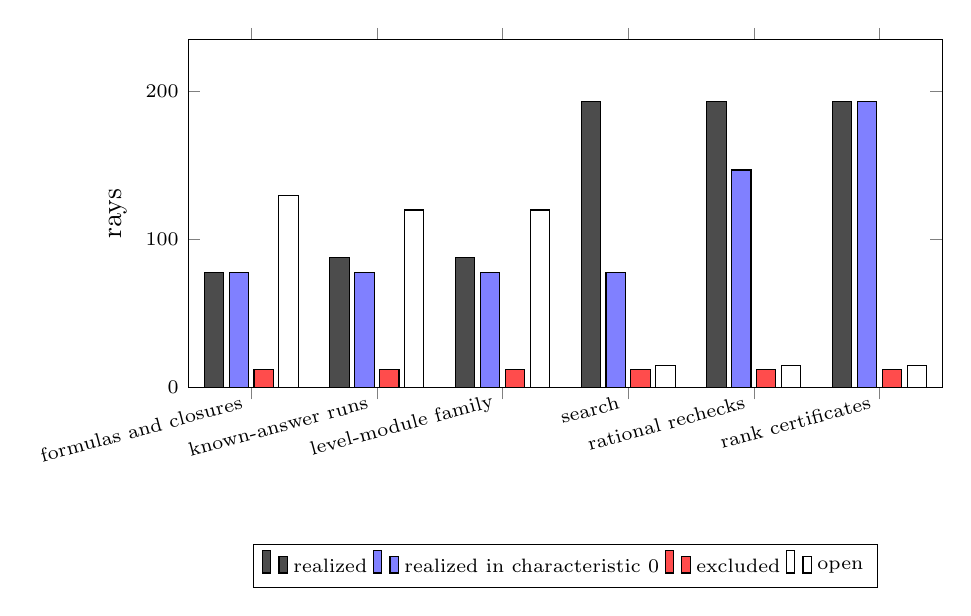
\begin{tikzpicture}
\begin{axis}[ybar, width=0.92\textwidth, height=6cm, bar width=7pt, ymin=0, ymax=235, symbolic x coords={formulas and closures,known-answer runs,level-module family,search,rational rechecks,rank certificates}, xtick=data, x tick label style={font=\scriptsize, rotate=15, anchor=east}, tick label style={font=\scriptsize}, ylabel={rays}, legend style={font=\scriptsize, at={(0.5,-0.45)}, anchor=north}, legend columns=4, enlarge x limits=0.1]
\addplot[draw=black, fill=black!70] coordinates {(formulas and closures,78) (known-answer runs,88) (level-module family,88) (search,193) (rational rechecks,193) (rank certificates,193)};
\addlegendentry{realized}
\addplot[draw=black, fill=blue!50] coordinates {(formulas and closures,78) (known-answer runs,78) (level-module family,78) (search,78) (rational rechecks,147) (rank certificates,193)};
\addlegendentry{realized in characteristic 0}
\addplot[draw=black, fill=red!70] coordinates {(formulas and closures,12) (known-answer runs,12) (level-module family,12) (search,12) (rational rechecks,12) (rank certificates,12)};
\addlegendentry{excluded}
\addplot[draw=black, fill=white] coordinates {(formulas and closures,130) (known-answer runs,120) (level-module family,120) (search,15) (rational rechecks,15) (rank certificates,15)};
\addlegendentry{open}
\end{axis}
\end{tikzpicture}

\caption{The number of rays in each class after each stage of the census; the stage with rational rechecks moves rays from realized over a prime field to realized in characteristic $0$ without changing the total, and the stage with the rank certificates gives the final table, carrying the remaining rays to characteristic $0$.}
\label{fig:stages}
\end{figure}

\emph{The excluded rays.} Twelve primitive points are excluded (Table~\ref{tab:excluded}); on each of them twice the primitive point is realized, so $c_d=2$. Ten pass the parity test and are the rays of Table~\ref{tab:ten} (without $(0,3,7,10)$), and two fail it, $(0,4,9,10)$ and $(0,1,6,10)$, which are the rays of Proposition~\ref{prop:least}.

\begin{table}[htbp]
\centering\footnotesize
\begin{tabular}{@{}lllll>{\raggedright\arraybackslash}p{3.6cm}@{}}
\toprule
ray & primitive point & $p(-1)$ & obstructions (O1 to O6) & $c_d$ & module over $U$\\
\midrule
$(0,1,3,4)$ & $(1,2,2,1)$ & 0 & O1, O2, O4 (dual: O1, O2, O4) & 2 & $k=U/U(x,y)=L(0,0)$\\
$(0,1,5,6)$ & $(2,3,3,2)$ & 0 & O1, O2 (dual: O1, O2) & 2 & $L(1,1)$\\
$(0,1,6,10)$ & $(6,8,3,1)$ & 16 & O2, O3 (dual: O1, O2, O5) & 2 & none ($p(-1)\ne0$)\\
$(0,1,7,8)$ & $(3,4,4,3)$ & 0 & O1, O2 (dual: O1, O2) & 2 & $L(2,2)$\\
$(0,1,9,10)$ & $(4,5,5,4)$ & 0 & O1, O2 (dual: O1, O2) & 2 & $L(3,3)$\\
$(0,1,11,12)$ & $(5,6,6,5)$ & 0 & O1, O2 (dual: O1, O2) & 2 & $L(4,4)$\\
$(0,2,6,8)$ & $(1,2,2,1)$ & 0 & O1, O2, O4 (dual: O1, O2, O4) & 2 & $U/U(x^2,y^2)$\\
$(0,2,10,12)$ & $(2,3,3,2)$ & 0 & O1, O2 (dual: O1, O2) & 2 & coker of a $2\times3$ matrix of quadrics\\
$(0,3,5,8)$ & $(1,4,4,1)$ & 0 & O4 (dual: O4) & 2 & $L(2,0)$\\
$(0,3,9,12)$ & $(1,2,2,1)$ & 0 & O1, O2, O4 (dual: O1, O2, O4) & 2 & $U/U(x^3,y^3)$\\
$(0,4,9,10)$ & $(1,3,8,6)$ & -16 & O1, O2, O5 (dual: O2, O3) & 2 & none ($p(-1)\ne0$)\\
$(0,5,7,12)$ & $(1,6,6,1)$ & 0 & O4 (dual: O4) & 2 & $L(4,0)$\\
\bottomrule
\end{tabular}

\caption{The \nexcluded{} rays with $d_3\le12$ whose primitive point is excluded over $S$: the primitive point, the parity value, the obstructions O1 to O6 that exclude it (with those of the dual ray), the least realizable multiple $c_d=2$ and the module over $U$ where the parity value is zero.}
\label{tab:excluded}
\end{table}

\emph{The open rays.} The \nopen{} open rays all have $d_3\ge10$ (Table~\ref{tab:open}); the largest upper bound on $c_d$ among them is \nopenMaxUp{} and only one of them passes the parity test, $(0,3,7,10)$, which is realized over $U$. A miss of a generic module on these rays proves nothing.

\begin{table}[htbp]
\centering\footnotesize
\begin{tabular}{@{}lllrrl@{}}
\toprule
ray & primitive point & $p(-1)$ & $c_d \ge$ & $c_d \le$ & dual ray\\
\midrule
$(0,3,6,10)$ & $(14,40,35,9)$ & 80 & 1 & 3 & $(0,4,7,10)$\\
$(0,3,6,11)$ & $(20,55,44,9)$ & 128 & 1 & 3 & $(0,5,8,11)$\\
$(0,3,7,10)$ & $(2,5,5,2)$ & 0 & 1 & 21 & $(0,3,7,10)$\\
$(0,3,7,11)$ & $(32,77,66,21)$ & 64 & 1 & 2 & $(0,4,8,11)$\\
$(0,3,7,12)$ & $(15,35,27,7)$ & 16 & 1 & 6 & $(0,5,9,12)$\\
$(0,3,8,11)$ & $(5,11,11,5)$ & 32 & 1 & 12 & $(0,3,8,11)$\\
$(0,3,8,12)$ & $(15,32,27,10)$ & 64 & 1 & 6 & $(0,4,9,12)$\\
$(0,4,7,10)$ & $(9,35,40,14)$ & -80 & 1 & 3 & $(0,3,6,10)$\\
$(0,4,7,11)$ & $(3,11,11,3)$ & -16 & 1 & 14 & $(0,4,7,11)$\\
$(0,4,7,12)$ & $(10,35,32,7)$ & -64 & 1 & 6 & $(0,5,8,12)$\\
$(0,4,8,11)$ & $(21,66,77,32)$ & 64 & 1 & 2 & $(0,3,7,11)$\\
$(0,4,9,12)$ & $(10,27,32,15)$ & -64 & 1 & 6 & $(0,3,8,12)$\\
$(0,5,8,11)$ & $(9,44,55,20)$ & 128 & 1 & 3 & $(0,3,6,11)$\\
$(0,5,8,12)$ & $(7,32,35,10)$ & 64 & 1 & 6 & $(0,4,7,12)$\\
$(0,5,9,12)$ & $(7,27,35,15)$ & -16 & 1 & 6 & $(0,3,7,12)$\\
\bottomrule
\end{tabular}

\caption{The \nopen{} rays whose primitive point is open over $S$: the primitive point, the parity value, the bounds on the least multiple $c_d$ (the lower bound from the obstructions, the upper bound from the constructions) and the dual ray; the search over $\F_{32003}$ found no hit on any of them.}
\label{tab:open}
\end{table}

\subsection{Rank certificates and the lift to characteristic \texorpdfstring{$0$}{0}}
\label{sec:lift-results}

The rank test was run on the \nfourHits{} verified hits of the census, with \nfourMatrices{} integer matrices in all. It reproduces the known answers: the pure Hilbert function over $\F_{32003}$ in every degree on every hit, the pass on \nfourKnown{} of \nfourKnown{} hits whose resolution over $\Q$ had given the pure table, \nfourAgree{} agreements of \nfourCompared{} between the two instruments on the matrices both computed (every matrix of at most $2{,}000$ rows and six larger ones), and \nfourUnitTests{} unit tests on modules with hand-computed Hilbert functions. The test passes with the first instrument on \nfourPassOne{} of the \nfourHits{} hits; on the last, python-flint reached its time limit on the matrix of $\nfourOneRows\times\nfourOneCols$ in degree $10$ on $(0,3,10,12)$, one degree above the top degree $9$ of the module, which the proposition does not need; its rank modulo $32003$ is $\nfourOneRows$, the number of rows, so its rank over $\Q$ is $\nfourOneRows$ as well (PARI/GP agrees). Among the \nfourRest{} hits without a completed positive rational recheck, \nfourRestPass{} pass with the first instrument and the last with the second. The largest matrix is $\nfourLargestRows\times\nfourLargestCols$, the longest rank over $\Q$ takes \nfourLongestSec{} seconds, and the rank certificates of all \nfourHits{} hits take \nfourTotalSec{} seconds of summed time, against two to thirty minutes for a resolution over $\Q$ and seven stops at the time limit (Table~\ref{tab:procedures}).

\emph{The two modules whose rational recheck gave no result.} The rational rechecks of $(0,3,8,10)$ and $(0,3,11,12)$ in Macaulay2 ended after about $110$ seconds without a result, before the resolution could finish (a later run of the same script needs $522$ seconds on the first, where it gives the pure table, and more than $900$ seconds on the second; these two run times are from the record of the independent check and are not archived [U]), and the run script recorded a run without a result as a failure. The prediction for the rank test on these two was that it would fail; it did not. Both pass, with equal ranks in every degree, and Proposition~\ref{prop:lift} says that the lifted modules are pure over $\Q$. Singular 4.3.2 over $\Q$, with scripts built from the saved generator matrices by code that shares nothing with the search, the recheck script or the rank test, gives $(7,16,21,12)$ on $(0,3,8,10)$ with length \nfourLenA{} and $(6,11,27,22)$ on $(0,3,11,12)$ with length \nfourLenB{}, the primitive points, with lengths equal to the sums of the Hilbert functions of the rank test (Table~\ref{tab:lift}). The recheck therefore completed on \nqqOk{} hits, all pure, and no hit of the census is known not to lift to characteristic $0$. What ended the two Macaulay2 runs is not established.

\begin{table}[htbp]
\centering\footnotesize
\begin{tabular}{@{}>{\raggedright\arraybackslash}p{2.1cm}>{\raggedright\arraybackslash}p{2cm}>{\raggedright\arraybackslash}p{1.8cm}>{\raggedright\arraybackslash}p{2.2cm}>{\raggedright\arraybackslash}p{2.2cm}rr@{}}
\toprule
ray & primitive point & Macaulay2 over $\mathbb{Q}$ & rank test & Singular over $\mathbb{Q}$ & length & seconds\\
\midrule
$(0,3,8,10)$ & $(7,16,21,12)$ & no result (run ended at about 110 s) & equal in all 9 degrees & $(7,16,21,12)$ & 280 & 426\\
$(0,3,11,12)$ & $(6,11,27,22)$ & no result (run ended at about 110 s) & equal in all 11 degrees & $(6,11,27,22)$ & 396 & 375\\
\bottomrule
\end{tabular}

\caption{The two hits whose Macaulay2 recheck over $\Q$ ended without a result: the rank test gives equal ranks over $\Q$ and $\F_{32003}$ in every degree, and Singular over $\Q$ gives the primitive point on each ray, with the length equal to the sum of the Hilbert function of the rank test and the time of the resolution in seconds.}
\label{tab:lift}
\end{table}

\emph{Field scope of the census.} Two numbers with their evidence give the scope (Table~\ref{tab:scope}). The primitive point is realized in characteristic $0$ on \nrealizedZero{} of the \nrealized{} rays by a cited construction or by a resolution over $\Q$ [V and MV]: \nrealizedEvery{} over every field or every infinite field, and \nrealizedZeroOnly{} in characteristic $0$. The other \nrealizedPrimeOnly{} rays are realized over $\F_{32003}$ by a hit of the search; the rank certificate and Proposition~\ref{prop:lift} carry all of them to characteristic $0$: \nfourDirect{} by a passing hit on the ray itself, among them $(0,3,10,12)$, and \nfourDual{} by the $\Ext^3$ dual of a passing hit on the dual ray, among them $(0,2,9,12)$, so that all \nrealized{} realized rays are realized in characteristic $0$ [D with MV]. The \nexcluded{} excluded and the \nopen{} open rays are unchanged.

\begin{table}[htbp]
\centering\footnotesize
\begin{tabular}{@{}>{\raggedright\arraybackslash}p{4.2cm}r>{\raggedright\arraybackslash}p{6.2cm}r@{}}
\toprule
group of rays & rays & evidence for the primitive point and its mark & in characteristic 0\\
\midrule
over every field or every infinite field & 52 & formula or classical complex, any field or infinite field [V]; scaling [D] & yes\\
characteristic 0 only & 95 & formula valid in characteristic 0, or a resolution over $\mathbb{Q}$ of a lifted hit, or its dual [V, MV] & yes\\
over $\mathbb{F}_{32003}$ by a hit of the search & 46 & hit, rank certificate and Proposition~\ref{prop:lift} [D, MV] & yes\\
total & 193 &  & 193\\
\bottomrule
\end{tabular}

\caption{Field scope of the \nrealized{} rays with $d_3\le12$ whose primitive point is realized over $S$, with the evidence for each group and its mark: the rays realized over every field or infinite field and in characteristic $0$ by a cited construction or a resolution over $\Q$ do not use the lift proposition, and the rays realized over $\F_{32003}$ only use it together with the rank certificate.}
\label{tab:scope}
\end{table}

\subsection{The rays with \texorpdfstring{$d_3\le9$}{d3<=9} and the two rays with \texorpdfstring{$d_3=10$}{d3=10}}

Table~\ref{tab:lownine} gives the evidence for the $84$ rays with $d_3\le9$: \nlowNineFormula{} by a formula, \nlowNineScaling{} by scaling, \nlowNineSocle{} and \nlowNineModule{} by explicit rational modules from the two generators, \nlowNineDual{} by $\Ext^3$ duals and \nlowNineExcluded{} over $U$; the field scope of the $79$ rays realized over $S$ is \nlowNineAny{} over every field, \nlowNineInfinite{} over every infinite field, and \nlowNineZero{} in characteristic $0$ only. The rational modules of the rays with $d_3\le9$ are archived: \nqqModules{} modules for \nqqRays{} rays, each pure over $\Q$ with the length equal to the Herzog--K\"uhl length, with the integer generator matrices, scripts and hashes (Table~\ref{tab:manifests}). The duals were computed directly over $\Q$ on \nqqDualsDirect{} of the $13$ duality rays; the other \nqqDualsClosure{} rest on the duality closure with the source module computed over $\Q$. Combined with the evidence for the five rays over $U$, this is Proposition~\ref{prop:lownine}, and with Proposition~\ref{prop:least} it gives the least counterexample: in characteristic $0$ none has $d_3\le9$, and the two dual rays $(0,4,9,10)$ and $(0,1,6,10)$ with $d_3=10$ are counterexamples over every field. In characteristic $2$ the ray $(0,2,6,8)$ has a counterexample with $d_3=8$ (Theorem~B); nothing is claimed for $d_3\le9$ in characteristic $p\ge3$.

\begin{table}[htbp]
\centering\footnotesize
\begin{tabular}{@{}>{\raggedright\arraybackslash}p{7.6cm}r>{\raggedright\arraybackslash}p{3.8cm}@{}}
\toprule
evidence for the primitive point & rays & field scope\\
\midrule
formula: Eisenbud--Schreyer, the two Eisenbud--Fl{\o}ystad--Weyman constructions, Koszul, $S/\mathfrak m^a$ and its dual, Buchsbaum--Rim, or generic Pfaffians & 35 & 26 any field, 3 infinite field, 8 characteristic 0 only\\
scaling of a formula ray (flat base change $x_i\mapsto x_i^2$) & 2 & any field\\
explicit module over $\mathbb{Q}$, level-module generator & 14 & characteristic 0\\
explicit module over $\mathbb{Q}$, generic presentation & 15 & characteristic 0\\
$\mathrm{Ext}^3$ dual of a module of the two previous rows & 13 & characteristic 0\\
excluded over $S$, realized over $U$ (Table~\ref{tab:ten}) & 5 & characteristic 0\\
total & 84 & 79 over $S$, 5 over $U$\\
\bottomrule
\end{tabular}

\caption{Evidence for the primitive point on each of the $84$ rays with $d_3\le9$, with the number of rays of each type and its field scope; the rays realized by formulas carry the field of the weakest construction they need, and the explicit modules are archived over $\Q$ with their integer matrices.}
\label{tab:lownine}
\end{table}

\subsection{Predictions that failed}
\label{sec:predfail}

Four predictions failed. The count of primitive points realized by formulas and closures at stage 0 was predicted between $52$ and $56$ and is \nstageZeroRealized{}: the $52$ realized over every field or every infinite field are as predicted, and the other \nstageZeroWeyman{} are rays where the second Eisenbud--Fl{\o}ystad--Weyman formula gives exactly $\beta_0$ in characteristic $0$, which the earlier tabulation of the programme (2026-09-02) did not count. The prediction that every prime-field hit persists over $\Q$ held: the rational recheck completed on \nqqOk{} hits, all pure, and the rank certificate passes on all \nfourHits{}. The prediction that the rank test would fail on the two hits whose rational recheck had been recorded as failed also failed: both pass, and Singular over $\Q$ gives the pure tables (Section~\ref{sec:lift-results}). The prediction that the rays with odd $d_1$ are hit in characteristic $2$ failed on $(0,3,9,12)$, which generic pairs of cubics realize over $\F_{32003}$ on $20$ of $20$ seeds and never in characteristic $2$, a finding that led to Theorem~C; the other such ray, $(0,5,7,12)$, is not reached by generic presentations over any field, six general quintics giving a non-pure table, so its characteristic $2$ outcome is not interpreted. The fourth failure is the share prediction of \EXP{006}: the share of random quartic spaces with $\operatorname{rank}\mu_{12}\le48$ was predicted between $0.3q^{-2}$ and $3q^{-2}$ in each of six fields, and it is \nsixRatioMin{} to \nsixRatioMax{} times $q^{-2}$ (Table~\ref{tab:sixcounts}), outside the interval in all six. The prediction rested on the expected codimension $2$ of the locus $D_4$ in $\operatorname{Gr}(2,9)$ given by the Thom--Porteous formula, and on a class $300\sigma_2+325\sigma_{1,1}$ computed from it. That assumption fails: besides the components through pure points, $D_4$ contains the resultant hypersurface of the spaces whose two forms have a common root modulo $z$, which has codimension $1$ and no pure point (Remark~\ref{rem:common}), so $D_4$ is reducible and about $1/q$ of the spaces over $\F_q$ lie in it. The conclusions drawn from the same derivation, that $D_4$ is not empty and that its components through pure points have dimension at least $12$, hold for the reasons of Theorem~\ref{thm:family}, and the heuristic comparison of the pure share with $q^{-2}$ concerns the pure locus and is not contradicted.

One statement of the known-answer check of \EXP{006} was inconsistent when it was written: it listed the pair $(x^3,y^3)$ over $\F_5$ both among the pairs that are pure and among those that are not. Since $5<2e=6$ the pair is not pure by Theorem~\ref{thm:A}; the check was run with that expectation, and the pair was found not pure, while over $\F_7$ it was found pure. The other predictions of Section~\ref{sec:expdesign} held, among them the exact set of primes at which $M_e$ is not pure, the non-purity of a general pair for $e\ge4$, and all those of \EXP{005}, \EXP{007} and \EXP{008}.

Of the predictions of the three later computations two failed, both of \EXP{009}, and none of \EXP{011} and \EXP{012}. The prediction that the linear family holds a pure member over $\F_p$ in each of the pairs with $e<p<2e$ failed at $(6,7)$: all \nlfSixSevenRankR{} members of rank $r$ over $\F_7$ and all \nlfYSixSevenRankR{} of rank $r$ among the $20{,}000$ sampled over $\F_{49}$ were examined, and none has the pure Hilbert function; it held at the six other pairs. The prediction that a pure member exists over $\F_p$ or $\F_{p^2}$ in the eight pairs with $p\le e$ failed in all eight (confidence $0.3$ for each): in $(4,3)$, $(5,3)$, $(6,3)$, $(6,5)$, $(7,3)$, $(7,5)$ and $(7,7)$ every member has rank below $r$, and at $(5,5)$ the \nlfFiveFiveRankR{} members of rank $r$ have no pure Hilbert function. The prediction that no member has rank above $r$ held in all fifteen pairs. The failures say that the family does not settle these characteristics, and nothing about other pairs of forms: pure pairs outside the family exist at $(4,3)$, $(5,3)$, $(5,5)$ and $(6,3)$ (Section~\ref{sec:resodd}).

Of the predictions of the second set several failed. In \EXP{010} the exploratory prediction that the stratum $S(7;0,1)$ holds a pure member at $(8,11)$ failed (all $17{,}689$ members, \nwcEEightElevenRankR{} of rank $r$, none with the pure Hilbert function), and the prediction of a pure member at $(8,5)$ failed in the five strata examined (\nwcEEightFiveExamined{} members, none with the pure Hilbert function); the predictions for $(8,13)$, $(8,3)$ and $(8,7)$ held, as did the predictions on the five open pairs, on the share, on the exclusion and on the characteristic dividing $m$. In \EXP{014} the prediction that the middle stratum holds a pure member failed at $(8,3)$ (all $484$ members examined, none with the pure Hilbert function) and at $(12,7)$ (sampled, none found), and held at the other nine pairs; the prediction that $S(5;0,4)$ holds a pure member at $e=9$ failed at $(9,11)$ and $(9,13)$ (none found among $300{,}000$ random members each) and held at $(9,7)$ and, for the rank, at $(9,5)$; the other predictions held, among them that of the stratum of the linear family at $e=9$. Before the computation the count of conditions of Theorem~\ref{thm:inv}(c) suggested that the prediction would fail at $e=8$, $10$ and $12$; it did not, which shows that the conditions of that count are not independent. In \EXP{013} no prediction failed. One acceptance criterion failed as first stated: the control at $(7,11)$ in $S(4;0,3)$ with $30{,}000$ random members found no pure member, although pure members exist there; the sample could not give the certainty that the criterion asked of it (about one member in $47{,}000$ is pure), and the limit of that one control was raised to $300{,}000$ before any later case was computed (Section~\ref{sec:resmid}). The statement that pure pairs of $(6,7)$ are absent in the linear family (Section~\ref{sec:reslf}) stands: the pair $(6,7)$ is settled by the search in the strata, in a stratum that does not contain the linear family.

In the third set no prediction of \EXP{015} or \EXP{017} failed: the twelve outcomes of P1 and the three of P2 of \EXP{015} hold, and the share of members that pass the filter lies within the factor of $p^{-(e-3)}$ that \EXP{017} predicted in all eight cases (the guards of the script of the paper read each outcome from the stored results). Three predictions of \EXP{016} failed (Section~\ref{sec:reslists}): the list at $(14,3)$, which P2 gave probability $0.7$, is empty; over $\F_9$ the lists at $e=8$ and $e=14$, which P4 gave $0.6$ each, are empty; and five lists over prime fields have more than $3p$ forms, against P5 ($0.7$). The pair $(14,23)$ is an unfinished enumeration, not a prediction that failed. No prediction of \EXP{018} failed (Section~\ref{sec:reslargest}); its one deviation is a memory error in the first run, resumed with a smaller cache. \EXP{015} and \EXP{017} both met the overflow error of the rank routine at $e=13$ and were resumed with a replacement that reduces each coefficient modulo $p$ (Sections~\ref{sec:reslinrule} and~\ref{sec:resfilter}). \EXP{017} was also run in two parts with the same runner (the exploratory family and the second instrument after the first part); it computes the Hilbert function only for the members that pass the filter, and it tests the first congruence on blocks before the exact test, and the two tests agree on every member that reached the exact test.

\FloatBarrier
\section{Validation by independent routes}
\label{sec:validation}

Every load-bearing statement is checked along at least two routes that share no code, and the paper marks which.

\paragraph{Two implementations of the census.} The census was implemented in Python with rational arithmetic and, independently, in Macaulay2; they agree on the primitive point and on the three construction numbers on all \nrays{} rays, with \ncyclic{} cyclic and \nparityPassing{} parity-passing rays, and reproduce the columns of the earlier tabulation of the programme (2026-09-02) on every row, except for the $26$ rays where the second Eisenbud--Fl{\o}ystad--Weyman formula is counted. The Eisenbud--Schreyer number of $(0,4,9,13)$ is $15400$ in both, that is the multiple $3080$.

\paragraph{Two systems for each hit, and a third where it completed.} Each of the \nverified{} verified hits (one per ray and multiple) was recomputed from its saved presentation in a fresh Macaulay2 process and in Singular, with no failure; for the rays with $d_3\le9$ the rational modules were recomputed in Singular by scripts written independently of the search code, which is how the archived file of rational modules was produced, and \nqqModules{} of \nqqModules{} are pure; the rational recheck completed on \nqqOk{} of the \nverified{} hits, all pure, and the rank certificate covers all \nverified{} (Section~\ref{sec:lift-results}).

\paragraph{Two instruments over $U$.} The exact library and Singular agree on $\nagreeTwo{}$ and $\nagreeThree{}$ modules in the two computations over $U$, with no disagreement; the Hilbert function recomputed from the Singular table equals the library's in every check. Neither route is a re-run of the other: the exact library builds the quotient by linear algebra in the PBW basis and the Tor complex from it, whereas Plural computes a Gr\"obner basis of the relations and a free resolution from that basis, and the two implementations of the census were written separately.

\paragraph{Exact recomputation of the proof.} The proof of Theorem~A is checked by exact computation in this paper (Table~\ref{tab:blocks}): the normal-ordering identity for $a,e\le9$ (\nnormalOrderingCount{} identities), the numerator $1-2t^e+2t^{3e}-t^{4e}$ divided by $(1-t)^2(1-t^2)$ for $e\le\nnumeratorE$, the dimension of every weight block for $e\le8$ over $\Q$ and over the primes up to $31$, and the table of products~\eqref{eq:mult}. Also recomputed are the two relations of Lemma~\ref{lem:trivial}, the vanishing of $r_1$ and $r_2$, the commutators of $x^2$ and $y^2$ in characteristic $2$, and the entry $x\cdot yx$ of the table.

\paragraph{Independent derivations and the archive of their machine checks.} The derivations of Theorems A, B and C were re-derived step by step and checked by independent code written from the relation $xy=yx+z$ alone; the proofs of Theorem~D and of Proposition~\ref{prop:linear} were checked independently in the same way. The machine checks of the characteristic $2$ theorem that this independent check ran (exhaustive pairs of quadrics and cubics over $\F_2$, random pairs of quartics to septics and matrices of forms over $\F_2$, $\F_4$ and $\F_{16}$, the shapes with $b=a+2$, the family at $e=6,7$) are archived as \EXP{005} (Section~\ref{sec:resfive}) with both instruments, and its counts agree with the counts of that reader on the exhaustive families ($\nfiveCobConst$ and $\nfiveCobGrow$ for cubics, $\nfiveCoaConst$ and $\nfiveCoaGrow$ for quadrics). The results of \EXP{005}, \EXP{006}, \EXP{007} and \EXP{008} were also re-tallied from the stored per-case records with code written separately from the routines of the experiments, and samples of the stored spaces were rebuilt from their stored bases and their Hilbert functions and Betti tables recomputed with the module construction of the library; the pairs printed in Table~\ref{tab:sixpairs} were rebuilt from their printed text with a separate parser, and this rebuild was repeated independently for the pairs of \EXP{006}; the tangent dimensions of \EXP{007} were recomputed with exact ranks from another implementation, and every value agreed. These recomputations are recorded with the computations, and their scripts are not archived ([U] as archived evidence); the script of this paper recomputes in its own arithmetic the Hilbert functions of the printed pairs, the ranks of $\mu_{3e}$ and the orbit dimensions of the explicit pairs over $\Q$, and stops when an artifact differs.

\paragraph{The later computations, rebuilt.} Each decisive result of \EXP{009}, \EXP{011} and \EXP{012} was rebuilt without the routine of the computation. For \EXP{009}, six members (those at $(6,11)$, $(7,11)$, $(7,13)$, $(4,5)$, $(4,7)$ and $(5,7)$) were rebuilt from their printed polynomials with a separate parser, checked to be the members that their parameters name, and their Betti tables were recomputed with the module construction of the library in pure Python (all pure, with lengths $216$, $343$, $343$, $64$, $64$, $125$); the rank of $\mu_{3e}$ was recomputed with python-flint for every member of $(5,5)$, $(6,5)$ and $(4,3)$ and for $400$ random members of $(6,7)$ and $(7,7)$: no member has rank above $r$, $212$ members of $(5,5)$ have rank $r$ as stored, none at $(6,5)$, $(4,3)$ and $(7,7)$, and $153$ of the $400$ members at $(6,7)$ against the stored share $918$ of $2{,}401$. For \EXP{011}, eight cases (six of family $T$ and two of family $G$) were rebuilt from the polynomials printed in the summary with a separate parser, the commutator recomputed and compared with $\lambda z^e$ for the printed $\lambda$, and the Betti tables recomputed in pure Python (all pure; lengths $125$, $343$, $343$, $343$, $729$, $729$, $729$, $125$), with no discrepancy. For \EXP{012}, five explicit cases (B at $(4,3)$, $(6,5)$, $(8,7)$, C at $(6,3)$ and D at $(7,3)$) were rebuilt from the text of the computation's design with a separate parser, the commutator compared with $-Dz$ computed from the data of Corollary~\ref{cor:cases} ($x^5y^5z$ up to sign at $(6,5)$ and $z^7-x^6y^6z$ at $(7,3)$), and the Betti tables recomputed (all pure; lengths $64$, $216$, $512$, $216$, $343$), with no discrepancy. The script of this paper recomputes in its own arithmetic the commutator of every pair of Tables~\ref{tab:central}, \ref{tab:critpairs} and~\ref{tab:critneg}, the quantity $D$ of every explicit pair from the data of the pair, and the Hilbert function, the length and the rank of $\mu_{3e}$ of every printed pair with $e\le13$; and it stops when an artifact differs. These recomputations are recorded with the computations; their scripts are not archived ([U] as archived evidence).

\paragraph{The proofs of the new theorems.} The derivation of each new theorem was checked step by step independently, with the statement checked against computation: Theorem~\ref{thm:central} on six pairs inside its hypotheses, at $(3,3)$, $(5,5)$, $(7,7)$ and $(9,3)$, with $A,B$ other than $x^e,y^e$ and $l_1,l_2$ other than $y,x$, and on six outside them; Theorem~\ref{thm:crit} on the pairs of cases B, C, D at $(4,3)$, $(6,5)$, $(8,7)$, $(6,3)$ and $(7,3)$ and on $180$ random pairs, the criterion being decided by another route than the one of Section~\ref{sec:critmethods}, with agreement with purity on every pair, and the acyclicity lemma checked against its source; Proposition~\ref{prop:central} on six small cases by brute force, with the centralizer theorem of Amitsur checked against its source; Theorem~\ref{thm:scale} on six cases of its own, two of them on modules that are not pairs, the freeness of $U_\varphi$ up to degree $21$ for $d=3$ and $24$ for $d=4$, and the pairs of degree $8$ over $\F_3$ and of degree $12$ over $\F_5$, both pure; these hand computations are not archived and the pull-backs are not printed in this paper [U as archived evidence]. The proof of Proposition~\ref{prop:strata} and the tables of Section~\ref{sec:strata} were reproduced stratum by stratum with independent code, which also gives the totals for $e=9$ and $e=10$ that the script of the paper recomputes (Section~\ref{sec:strata}).

\paragraph{The second set of later computations, rebuilt.} For \EXP{010}, in a first part nine decisive members were rebuilt from the printed polynomials with a separate parser, checked to lie in their strata and tabled with the module construction of the library (all pure); the stratum $S(6;0,3)$ over $\F_7$ was recounted with an own enumeration and rank routine ($3{,}200$ members, $588$ of rank $r$, $12$ with the pure Hilbert function); a stratum that is not admissible was sampled with own code. In a second part, after the run, the first two pure members of every stratum with a pure member at $(7,7)$, $(8,3)$, $(8,7)$, $(8,13)$ were rebuilt from the stored coefficient vectors, checked to lie in their strata and tabled: $22$ members in $11$ strata, all pure, of lengths $343$ and $512$. For \EXP{013}, $S2$, $S3$ and $T1$ were rebuilt with a separate substitution ($x\mapsto\varphi(x)$, $y\mapsto\varphi(y)$, $z\mapsto\varphi(x)\varphi(y)-\varphi(y)\varphi(x)$, monomial by monomial) and the Betti tables of $M'$ and of its pull-back recomputed in pure Python: the table is the scaled table and the length is $d^3$ times, in the three cases ($512$, $1{,}728$, $81$). For \EXP{014}, the first two pure members of each of the eleven cases of families V and W with a pure member were rebuilt from the stored coefficient vectors with a separate parser, checked to lie in their strata and tabled (all pure; lengths $512$, $729$, $1{,}000$, $1{,}728$), and the stratum $S(8;0,4)$ over $\F_5$ was recounted with an own enumeration and rank routine ($4{,}686$ members, $436$ of rank $r$, $4$ with the pure Hilbert function). The script of the paper checks the stratum of every printed pair of Tables~\ref{tab:wcpairs} and~\ref{tab:midpairs}, recomputes the Hilbert function, the length and the rank of $\mu_{3e}$ of the pairs with $e\le10$, and recomputes the substitution of Section~\ref{sec:pbmethods} for every case; the counts of the totals are checked against the sum over the strata. These recomputations are recorded with the computations and their scripts are not archived ([U] as archived evidence).

\paragraph{The congruence, the Betti table and the existence.} Theorem~\ref{thm:cong} was checked on every monic form over the prime field in eleven cases, with polynomial arithmetic only: the forms, those with (C), those with (C) and the condition at $r=0$, and those with all conditions are $169,101,16,16$ at $(4,13)$; $289,196,13,13$ at $(4,17)$; $125,40,2,2$ at $(6,5)$; $343,156,2,2$ at $(6,7)$; $1331,552,4,4$ at $(6,11)$; $2197,969,0,0$ at $(6,13)$; $4913,2661,2,2$ at $(6,17)$; $625,195,1,1$ at $(8,5)$; $2401,798,4,4$ at $(8,7)$; $14641,6107,1,1$ at $(8,11)$; $28561,11715,1,1$ at $(8,13)$ ($55{,}595$ forms, $23{,}490$ of them with (C)); no form with (C) has the condition at $r=0$ without the full set. Theorem~\ref{thm:betti} was checked on the $42$ forms with (C) and the congruence at $(4,7)$, $(4,11)$, $(4,13)$, $(4,17)$, $(6,5)$, $(6,7)$, $(6,11)$, $(6,17)$ ($1,2,16,13,2,2,4,2$ forms), written in the monomials of the library with $f=x^e+y^e$: length $e^3$ and the table $(1,2,2,1)$ in every case by the module construction of the library, and on forty forms with (C) and without the congruence (five per case) the length is $63$ instead of $64$ at $e=4$ and $212$ or $213$ instead of $216$ at $e=6$. Theorem~\ref{thm:exist} was checked by power series to order $8$ (the remainder of $\Gamma(\xi-2e)\kappa_e-\nu\Gamma(\xi+2e)\pi_e$ modulo $\Gamma$ vanishes to that order and every $c_i$ is not zero) for $e=4$ with $S=\{1,3\},\{1,2\},\{2,4\}$, $e=6$ with $\{1,3,5\},\{2,3,6\}$ and $e=8$ with $\{1,3,5,7\}$ over the rationals, and for $(e,p)=(4,7)$, $(6,11)$, $(10,19)$, $(12,23)$, $(16,31)$ with the odd numbers below $e$; at $e=4$ the coefficients $(\alpha,\gamma)$ of $\Gamma=\xi^2+\alpha\xi z+\gamma z^2$ satisfy the quintic of Remark~\ref{rem:invariants} to order $8$ in the three cases. An independent check, with code written separately from that of the computations, verified Theorem~\ref{thm:cong} and the description of (C) by roots on every monic form in ten cases; computed in $U$, without the decomposition, the length of all $2{,}190$ forms with (C) at $(4,19)$, $(4,23)$, $(6,11)$, $(6,13)$, $(8,3)$ (length $e^3$ exactly for the forms with the congruence); tabled $87$ forms with (C) and the pure Hilbert function over $\F_p$, $\F_{p^2}$, $\F_{32003}$ and the rationals, all pure, nine of them also in Singular; built, from the branch of Theorem~\ref{thm:exist} at $(4,7)$ (it lies on a quartic factor of the quintic modulo $7$), the pair $x^4+y^4$, $x^2y^2+5xyz+4z^2$ over $\F_7$ and, over $\F_{49}$, $33$ forms, for example $x^4+y^4$, $x^2y^2+4a\,xyz+a\,z^2$ with $a^2=-1$, both pure; and checked (H1) for the odd numbers below $e$ at all $499$ pairs with $e\le40$ and $2e<p<8e$ and at $p=2e-1$ for every even $e\le40$, and the count of Remark~\ref{rem:exist}(1) for every even $e$ up to $40$. These are hand computations whose scripts and logs are kept under the data root of the programme (the folder of \EXP{014}, a subfolder of the independent check, and a second folder of independent checks), not archived in the repository [U as archived evidence]; they are not artifacts that the script of the paper reads.

\paragraph{The projection on the weight-zero summand.} The counts on which Corollary~\ref{cor:wzstrata} is used are recomputed by the script of the paper from the definitions: \nwzExcluded{} strata of the stored searches are excluded, holding \nwzExcludedMembers{} members of which \nwzExcludedRankR{} have rank $r$ and none has the pure Hilbert function; \nwzExcludedAdm{} admissible strata remain with $p$ not dividing $m$; the stratum $S(8;0,1)$ at $(9,11)$ and $(9,13)$ of \EXP{014} (\nwzExcludedFourteen{} members) and the \nwzExcludedFifteen{} excluded strata of \EXP{015} (\nwzExcludedFifteenMembers{} members) hold no pure member. The machine checks of the projection (the examples of Remark~\ref{rem:proj}) were run by hand and are not archived [U as archived evidence]; the corollaries are proved on paper.

\paragraph{The lists of forms.} Every one of the \nlstVerified{} listed forms checked in $U$ is pure with length $e^3$ in two instruments (Singular with Plural and the first instrument of the paper); the form of each of the \nlstEFourteenMembers{} pure members stored by \EXP{014} at the five pairs that the lists also cover lies in its list, so the lists are consistent with an independent search; for the first form of every list that is not empty, and for the second form at the pairs not settled before, a test of (C) by greatest common divisors, the congruence, a separate conversion of the polynomial and the Betti table by a second module construction were run without the routine of the computation, on $30$ forms at $21$ pairs, with no finding [U as archived evidence]. The theorem that the lists rest on (Theorem~\ref{thm:cong}) was checked independently on $87$ further forms [U as archived evidence].

\paragraph{The strata with the largest exponent.} The five strata of family Z of \EXP{018}, where Corollary~\ref{cor:wzstrata} applies, were fixed before the run as a test of the corollary and hold no member with the pure Hilbert function among $50{,}000$ each; the $21$ members of the sample are pure in two instruments; and the first two pure members of each of the seven cases with a pure member were rebuilt from the stored coefficients with a separate parser, checked to lie in the stratum of their case and tabled by a second module construction ($14$ members, lengths $729$, $1331$, $2197$ and $2744$, no finding) [U as archived evidence].

\paragraph{The rule and the filter.} The twelve pairs of \EXP{015} are recomputed by the script of the paper (the pairs by the instrument of the paper, the Hilbert function, the length and the rank of $\mu_{3e}$) and the exclusion half of the rule is also proved (Corollary~\ref{cor:linstratum}), so the computation and the proof agree on every pair with $2e-p\ge5$. For the filter, the control cases on settled pairs agree with the pairs found before, and all $\nfltTables{}$ tables computed are pure; the converse (that a member that fails the filter is not pure) is not tested here.

\paragraph{The decomposition and the characteristic dividing $m$.} The proposition of Section~\ref{sec:invariants} was recomputed in the four ranges of $n$ and the Hilbert function it predicts was compared with the one computed in $U$ on $627$ forms at $(e,p)=(4,5)$, $(4,7)$, $(4,13)$, $(6,5)$, $(6,7)$ with no difference, and on every form at $(4,3)$, $(4,11)$, $(4,17)$, $(8,3)$, on $150$ forms at $(6,11)$ and on $376$ forms in characteristic $0$ for which the hypothesis (C) fails, with own code, with no difference. An independent count for $e=8$ over the prime field, evaluating the conditions of Theorem~\ref{thm:inv} for every monic form $\Gamma$, found the forms of the pure pairs of the middle stratum (Section~\ref{sec:resmid}). The proof of Proposition~\ref{prop:pdivm} was checked step by step, the syzygy built explicitly in four cases, and the bound tested on $941$ random pairs at $(4,3)$, $(9,3)$, $(9,5)$, $(9,7)$, $(10,7)$, $(11,11)$ and, for $p=2$, at $(4,2)$, $(5,2)$, $(6,2)$ [U as archived evidence].

\FloatBarrier
\section{Ablation and negative controls}
\label{sec:ablation}

Table~\ref{tab:controls} lists the controls and what each one caught. The controls are the part of the design that could have failed.

\begin{table}[htbp]
\centering\footnotesize
\begin{tabular}{@{}>{\raggedright\arraybackslash}p{4.3cm}>{\raggedright\arraybackslash}p{3.1cm}>{\raggedright\arraybackslash}p{6.1cm}@{}}
\toprule
control & what it tests & outcome\\
\midrule
known-answer modules before any claim & instruments and conventions & 17 modules of EXP-002 and 11 of EXP-003 reproduce their expected tables; the two instruments agree on 96 and 127 finite length modules\\
a hit on a point excluded by O1 to O6 & obstructions and constructions & none in the 2{,}996 cells of the search and the flags\\
lift of each hit to $\mathbb{Q}$ & persistence of a prime-field hit & 64 rechecks completed, all pure; the runs on $(0,3,8,10)$ and $(0,3,11,12)$ ended without a result and were recorded as failures; the rank test passes on both and Singular over $\mathbb{Q}$ gives the pure tables\\
first version of the rational recheck script & the recheck itself & a shadowed variable made 59 fresh-process records fail; they were discarded and recomputed\\
positive control over $\mathbb{F}_{32003}$ for the characteristic 2 searches & reach of generic presentations & seven of the eight rays hit on 20 of 20 seeds, against zero hits in characteristic 2 on $(0,3,9,12)$ and $(0,2,10,12)$; $(0,5,7,12)$ is not hit in any field\\
pairs of quadrics over $\mathbb{F}_3,\dots,\mathbb{F}_{81}$ & Hilbert function as a certificate & 60 pairs have the Hilbert function $(1,2,2,2,1)$, 54 of them have the table $(1,2,2,1)$ and 6 have extra Betti numbers\\
a general pair of forms of degree $e$ & whether $(x^e,y^e)$ is special & pure for $e=2,3$ on 5 of 5 pairs each; pure on 0 of 15 pairs for $e=4,5,10$\\
generic modules over $\mathbb{F}_2$, $\mathbb{F}_3$, $\mathbb{F}_5$ for the 130 verified generators & small-characteristic behaviour of the search & at least one of five seeds is pure on 98, 126 and 130 generators; a miss is a flag and no statement\\
\bottomrule
\end{tabular}

\caption{Controls and negative controls of the computations: what each one tested and the outcome, read from the archived records; the controls that failed (two lifts to $\Q$, one script defect) identify the claims that are weaker than a first reading.}
\label{tab:controls}
\end{table}

\paragraph{The recheck over $\Q$ and its first script.} The first pass of the rational recheck used a script with a variable shadowed by a ring variable, which made the fresh-process checks fail on \ndiscarded{} records; they were discarded and recomputed after the repair, and the Singular results, which read the saved presentation, were unaffected. A first failure of the rational recheck of $(0,1,2,3)$ was a second defect of the script (integer entries not promoted to the ring), repaired and rerun. After the repair, \nqqOk{} rechecks completed, all pure over $\Q$; \nqqFailed{} runs ended without a result (recorded as failures by the run script), $\nqqTimeout$ stopped at the thirty minute limit and \nqqNotRun{} were not reached. The two runs without a result are decided by the rank test and by Singular over $\Q$ (Section~\ref{sec:lift-results}). The lesson is that a run without a result line must be recorded as undecided, not as a failure.

\paragraph{Lifting the saved presentation is not the rational recheck.} For hits of the level-module generator the rational module is the image of the lifted generator matrix inside the truncated ring, as in Algorithm~\ref{alg:recheck}; the cokernel of the saved prime-field presentation lifted termwise to $\Q$ was not pure in the controls we ran on socle hits (this control was run by an independent reader and is not archived [U]). For this reason the rational modules of the rays with $d_3\le9$ are archived with their integer matrices and hashes (Table~\ref{tab:manifests}).

\paragraph{The Hilbert function does not certify purity.} Over $\F_3,\dots,\F_{81}$, \npairsRightHFWrongTable{} of the \npairsRightHF{} pairs of quadrics with the Hilbert function $(1,2,2,2,1)$ have a table with extra Betti numbers in degree $7$; for example over $\F_9$ two pairs have the table $(0,0,1),(1,2,2),(2,6,2),(2,7,1),(3,7,1),(3,8,1)$ instead of $(0,0,1),(1,2,2),(2,6,2),(3,8,1)$, written as triples $(i,j,\beta_{i,j})$. The socle in degree $3$ gives a $\Tor_3$ in degree $7$ (equation~\eqref{eq:tor3}), which is why the paper certifies purity through the socle and the Euler series and not through the Hilbert function.

\paragraph{A general pair for $e\ge4$.} For $e=2,3$ a random pair of forms of degree $e$ over $\F_{32003}$ is pure on \ngeneralPureTwoThree{} of \ngeneralPairs{} pairs each; for $e=4,5,10$ it has the maximal-rank Hilbert function and is pure on $0$ of \ngeneralPairs{} pairs each (Table~\ref{tab:controls}): the family $M_e$ is not found by a random search for $e\ge4$, as the Hilbert series predicts, and the pure points $(1,2,2,1)$ on $(0,e,3e,4e)$ are realized by a special left ideal. A random search over $\F_{32003}$ is therefore not a valid test of realizability for these rays. Over small fields the same search succeeds because the share of pure spaces, of the order of $q^{-2}$ by the heuristic of Section~\ref{sec:resodd} [C], is between about $10^{-1}$ and $10^{-3}$ there, whereas over $\F_{32003}$ it is of the order of $10^{-9}$, out of reach of the \ngeneralPairs{} random pairs tried.

\paragraph{The positive control over $\F_{32003}$.} The characteristic $2$ searches have a control: a ray not hit over $\F_{32003}$ is not reachable by generic presentations, and its characteristic $2$ outcome is not interpreted ($(0,5,7,12)$). The two rays hit over $\F_{32003}$ and never in characteristic $2$, $(0,3,9,12)$ and $(0,2,10,12)$, are the two where Theorem~C applies, which turns a pattern of misses into an exclusion.

\paragraph{Characteristic flags.} Generic modules for the \nflagGen{} verified generators were redrawn over $\F_2$, $\F_3$ and $\F_5$ with five seeds each; at least one seed gives the pure table on \nflagTwo{}, \nflagThree{} and \nflagFive{} of them. The primitive point was never hit over $\F_2$ on \nflagRaysTwo{} rays and over $\F_3$ on \nflagRaysThree{} rays, among them $(0,1,2,6)$, which is realized over every field by a formula: a miss of a generic module over a small field is a flag and not a claim.

\paragraph{Each hypothesis of the new theorems is used.} Table~\ref{tab:centralneg} lists the five pairs of \EXP{011} outside the hypotheses of Theorem~\ref{thm:central}, and Table~\ref{tab:critneg} the three pairs of \EXP{012} built to violate the criterion; the script recomputes the commutator of each. With $l_1=0$ ($x^5$, $y^5+xz^2$ at $(5,5)$), with $l_1,l_2$ dependent ($x^5+yz^2$, $y^5+yz^2$ at $(5,5)$) and with $\bar A,\bar B$ having a common factor ($yz^4+x^9$, $xz^4+x^6y^3$ at $(9,3)$) the commutator is a multiple of $z^e$ in the last case and not in the first two, and the module is not of finite length within degree $5e$ in all three; with $p\nmid e$ (the same pair $x^5+yz^2$, $y^5+xz^2$ at $(5,7)$ and $(5,3)$) $A$ and $B$ are not central, none of the identities holds, and the Hilbert function is not $h_e$. In the criterion, case D without the term $x^3z^2$ at $(7,3)$, the pair $x^6$, $y^6+z^3$ at $(6,5)$ (where $n(f)=X^6$ vanishes on $X=0$, where $zD$ vanishes) and case C without $z^3$ at $(6,3)$ fail the criterion, and none of the three modules has finite length within degree $5e$. So dropping any one of the hypotheses of Theorem~\ref{thm:central} (independent linear forms, forms without common factor, $p$ dividing $e$) or of Theorem~\ref{thm:crit} (the term that keeps the common zeros apart) gives a module that is not pure in the cases tried [MV].

\begin{table}[htbp]
\centering\footnotesize
\begin{tabular}{@{}ll>{\raggedright\arraybackslash}p{5.0cm}>{\raggedright\arraybackslash}p{3.0cm}ll@{}}
\toprule
case & $(e,p)$ & forms over $\F_p$ & outside the hypotheses because & $gf-fg=\lambda z^e$ & finite length\\
\midrule
N1 & $(5,5)$ & $f=x^{5}$\newline $g=xz^{2} + y^{5}$ & $l_1=0$ & no & no\\
N2 & $(5,5)$ & $f=x^{5} + yz^{2}$\newline $g=yz^{2} + y^{5}$ & $l_1,l_2$ dependent & no & no\\
N3 & $(5,7)$ & $f=x^{5} + yz^{2}$\newline $g=xz^{2} + y^{5}$ & $p\nmid e$ & no & no\\
N4 & $(5,3)$ & $f=x^{5} + yz^{2}$\newline $g=xz^{2} + y^{5}$ & $p\nmid e$ & no & no\\
N5 & $(9,3)$ & $f=x^{9} + yz^{4}$\newline $g=x^{6}y^{3} + xz^{4}$ & $\bar A,\bar B$ with a common factor & yes & no\\
\bottomrule
\end{tabular}

\caption{The five pairs outside the hypotheses of Theorem~\ref{thm:central}: the case, $(e,p)$, the forms over $\F_p$, what places the pair outside the hypotheses, whether $gf-fg$ is a multiple of $z^e$ (computed by the script) and whether the module has finite length within degree $5e$ (it does not in any case).}
\label{tab:centralneg}
\end{table}

\begin{table}[htbp]
\centering\footnotesize
\begin{tabular}{@{}ll>{\raggedright\arraybackslash}p{4.6cm}>{\raggedright\arraybackslash}p{4.2cm}l@{}}
\toprule
case & $(e,p)$ & forms over $\F_p$ & built to violate & finite length\\
\midrule
N1 & $(7,3)$ & $f=x^{7} + yz^{3}$\newline $g=xz^{3} + y^{7}$ & case D without the term $x^3z^2$ & not within degree $35$\\
N2 & $(6,5)$ & $f=x^{6}$\newline $g=z^{3} + y^{6}$ & $n(f)=X^6$ vanishes on $X=0$ where $zD$ vanishes & not within degree $30$\\
N3 & $(6,3)$ & $f=x^{6} + y^{4}z$\newline $g=x^{4}z + y^{6}$ & case C without $z^3$ & not within degree $30$\\
\bottomrule
\end{tabular}

\caption{The three pairs of the class $V_e$ built to violate the criterion of Theorem~\ref{thm:crit}: the case, $(e,p)$, the forms over $\F_p$, how the pair violates the criterion, and the outcome: none has finite length within degree $5e$; the script recomputes $gf-fg=-Dz$ for each.}
\label{tab:critneg}
\end{table}

\paragraph{Strata that are not admissible.} The necessary condition of Proposition~\ref{prop:strata} removes most strata at $e=4,\dots,8$ (Table~\ref{tab:stratatot}), and the containment remark removes the strata with $m=e$ and $i,j\ge1$: a pure pair cannot lie in them. The part of the stratum $S(e-1;0,1)$ outside the chart of the linear family holds no pure pair in any characteristic (Section~\ref{sec:strata}), so a pure pair of that stratum is a member of the family.

\paragraph{Outside the hypotheses of the new statements.} The two cases of \EXP{013} outside the hypotheses of Theorem~\ref{thm:scale} fail as the theorem predicts: the $p$-th power map is not an endomorphism of finite colength and its pull-back is not pure, and a substitution that is not an endomorphism does not rescale the table (Section~\ref{sec:respull}) [MV]. The exclusion of Proposition~\ref{prop:strata} was tested on the strata that are not admissible (Section~\ref{sec:resstrata}): none of the \nwcNonAdm{} strata holds a member with the pure Hilbert function among \nwcNonAdmMembers{} members. The rank of the members of the strata with $p$ dividing $m$ was tested against Proposition~\ref{prop:pdivm} in sixteen pairs. In Theorem~\ref{thm:inv} the hypothesis (C) is used: forms without (C) that have the pure Hilbert function exist and none of the computed cases has a pure Betti table (Remark~\ref{rem:invariants}(4)), and without (C) the proposition still gives the Hilbert function but the theorem says nothing. In the strata, an enumeration of a stratum cut by the early stop proves nothing about the members after the cut, and a sampled stratum without a pure member is ``none found'': $(9,11)$ and $(9,13)$ in the middle-stratum search and $(12,7)$ in its sample were later settled by other strata and by the list of forms.

\subsection{Controls of the later computations}
\label{sec:ablation3}

\EXP{015}: four controls with known answers (the stratum of the linear family at $(9,17)$ and $(8,13)$ holds pure pairs, at $(9,13)$ and $(8,11)$ none) are run before the twelve pairs, and the strata that Corollary~\ref{cor:wzstrata} excludes are searched as controls of the corollary: none of them holds a member with the pure Hilbert function (\nwzExcludedFifteen{} strata, \nwzExcludedFifteenMembers{} members). \EXP{017}: the control cases $(5,7)$, $(7,5)$, $(7,11)$ and $(9,7)$ are settled pairs on which the filter is run first; of the stored members of the stratum with a computed table, the \nstmPure{} pure ones pass the filter and the \nstmOther{} others fail it, so the filter separates the stored pure members from the stored members with another table, and all \nfltTables{} tables computed through it are pure. \EXP{016}: the negative controls are the fifteen forms with (C) and without the congruence at $(6,7)$, $(8,5)$ and $(8,13)$, whose modules have length $212$ at $e=6$ and between $502$ and $507$ at $e=8$, never $e^3$; the lists of the pairs of $e\le10$ settled before have the sizes fixed in advance; the complete enumerations without a form (the lists at $(14,3)$, $(14,5)$, $(14,11)$ and over $\F_9$ at $e=8$ and $e=14$) say that no pair of that shape with (C) is pure over those fields, and nothing beyond that shape. The case $(14,23)$ is a control of the opposite kind: an unfinished enumeration is not a negative result. \EXP{018}: the two controls with known answers (the strata $S(7;0,2)$ at $(9,11)$ and $S(6;0,3)$ at $(9,13)$) give pure pairs, and the five strata with $t+2$ at the five pairs are negative controls fixed before the run, from the corollary: none holds a member with the pure Hilbert function among $50{,}000$. [MV]


\FloatBarrier
\section{Discussion}
\label{sec:discussion}

\subsection{What the dependence on the characteristic means for the question}

Question~6.1 is stated over a field $k$ without fixing the characteristic. The point $(1,2,2,1)$ on $(0,2,6,8)$ gives an answer that depends on $k$: realized over $U$ when $\ch k=0$ or $\ch k\ge5$ (by $U/U(x^2,y^2)$) and in characteristic $3$ (by explicit pairs), and realized over neither ring when $\ch k=2$. The same holds on $(0,e,3e,4e)$ for every $e\ge2$ in characteristic $0$ against characteristic $2$. This is a different phenomenon from the one used to answer the question negatively in 2026: the point of Jiang, Li, Sun, Wang, Xiao and Yu is excluded by a numerical test on the Hilbert series and so in every characteristic at once, whereas the points here pass that test and the exclusion comes from the structure of $U$, in a single characteristic. The consequence is that a negative answer to Question~6.1 does not settle which points are realized: the table of realizable points depends on the characteristic, as Kunte found for Betti tables of Cohen--Macaulay modules in five variables~\cite{Kunte}, and the census over $S$ already records the field scope of every realization.

For odd characteristic the picture is now settled for $e\le10$ and partly for larger $e$: the stratum of the linear family holds no pure pair for $p\le2e-5$ (a theorem), pure pairs exist in the computed cases with $2e-p\le3$, the filter of Section~\ref{sec:resfilter} reaches pairs, such as $(11,7)$ and $(13,5)$, that no theorem and no earlier search reached, the lists of forms settle $e=12$ and several pairs at $e=14$ and $e=16$ by one congruence, and the stratum with the largest exponent that the weight-zero projection allows settles five more pairs, among them $(11,13)$, $(11,17)$ and $(14,23)$. In characteristic $p$ odd the elements $x^p$, $y^p$ and $z$ are central and $U$ has rank $p^2$ over the subring they generate; no exclusion of the type of Theorem~C holds, and the structure of the centre gives pure pairs instead (Theorem~\ref{thm:crit}): pairs of forms with the pure table exist in every odd characteristic below $2e$ for $e=2,3,4,5$ (Corollary~\ref{cor:ray}), by explicit pairs and not by $(x^e,y^e)$, which fails there by Theorem~A. So on the rays $(0,e,3e,4e)$ with $2\le e\le10$ the point is realized over $U$ exactly when $\ch k\ne2$ (for $e\le5$ by explicit pairs found in the whole space, for $6\le e\le10$ with the searches in the strata and the criteria of Corollary~\ref{cor:eight}), and characteristic $2$ is the only characteristic that matters for them. At $e=6$ the point is realized in characteristics $3$, $5$, $7$ and $11$, at $e=7$ in $3$, $5$, $7$, $11$ and $13$, and at $e=8$ in $3$, $5$, $7$, $11$ and $13$ (Corollary~\ref{cor:eight}); Tables~\ref{tab:state} and~\ref{tab:statesrc} and Figure~\ref{fig:grid} give the state for larger $e$. Theorem~A answers it for $p\ge2e$ and the characteristic $2$ theorem for $p=2$. Whether characteristic $2$ remains the only exclusion for every $e$ is not known; the family of Theorem~D, of dimension at least $4e-4$ in $G_e$, makes it plausible that pure pairs exist over small fields in general, but a locus that is not empty over the algebraic closure may have no point over a given prime field, and the plausibility is not a statement [C].

\paragraph{What settles which pairs.} Three kinds of statement now settle the pairs of Tables~\ref{tab:statesrc} and~\ref{tab:statesrcb}. Theorems: the central pairs (the primes dividing $e(e-1)$), the pull-back and the scaling, and, in the other direction, the exclusions of the projection on the weight-zero summand and of the characteristic dividing the modulus. Pairs found in the stratum with the largest allowed exponent, by one congruence in the middle stratum and, for all $e$ up to $16$ that were run, by the lists of forms, in the stratum of the linear family when $2e-p\le3$, and in the strata at $e=9$: exact pairs over $\F_p$ whose purity is computed. And the filter, a criterion read off computed cases that is used only to choose members. The searches in the strata find pairs and prove nothing about the pairs they do not find; the exclusions prove the absence of pairs in their strata, and the rule of the linear family is the case where the two meet: no pure pair when $2e-p\ge5$, pure pairs in the computed cases when $2e-p\le3$.

\subsection{The mechanism, and why it stops at \texorpdfstring{$p\mid e(e-1)$}{p divides e(e-1)}}

The explicit pairs of this paper have one mechanism. A pair $(f,g)$ whose commutator $c=gf-fg$ is central has the four term sequence~\eqref{eq:FR} as a complex; when $\mathcal Z$ is the centre and the fibres of that complex over the points of $\operatorname{Spec}\mathcal Z$ away from the origin are exact, the complex is a resolution, and the module has the Hilbert series of a complete intersection of type $(e,e,2e)$ in $k[x,y,z]$ whose third relation, $z^e$ or $Dz$, is the commutator of the first two. Over the polynomial ring such a quotient needs three relations and has the Betti table $(1,3,3,1)$; over $U$ the commutator costs no generator, the Koszul relation between $f$ and $g$ of degree $2e$ is lost with it, and what is left is $(1,2,2,1)$ on $(0,e,3e,4e)$ (Remark~\ref{rem:mech}). The mechanism is exactly the base change of the resolution of the trivial module along an endomorphism of $U$ (Proposition~\ref{prop:endo}), and the endomorphisms that make $U$ a free module over itself exist in characteristic $p$ if and only if $p$ divides $d(d-1)$ (Corollary~\ref{cor:scale3}): a nonzero central commutator is a polynomial in $x^p$, $y^p$ and $z$ divisible by $z$, of degree $2e$, whose class modulo $z$ is the Jacobian determinant of the images of $f$ and $g$, a polynomial in $x^p$, $y^p$ of degree $2e-2$ that is nonzero only if $p$ divides $2e-2$, and vanishes only if $p$ divides $e$ (Theorem~\ref{thm:mech}(ii)). That is why the explicit pairs stop at the primes dividing $e(e-1)$, and why in characteristic $0$ no pair of degree $e\ge2$ has this mechanism: the centre is $k[z]$ and $z^e$ is not in the ideal of two forms without common factor (Proposition~\ref{prop:zpower}). In the other odd characteristics below $2e$ the pure pairs found by search (for example at $(5,7)$) have a commutator that does not commute with the pair (Theorem~\ref{thm:mech}(iii)), and what such a pure pair looks like is not known.

The comparison with the polynomial ring is instructive. Over $k[x,y,z]$ every $d\ge2$ rescales the degrees of a Betti table, in every characteristic, through $x_i\mapsto x_i^d$ (Section~\ref{sec:realizability}); over $U$ the same operation exists only in characteristic $p$ and only for $d\equiv0$ or $1\pmod p$, and not at all in characteristic $0$ (Corollary~\ref{cor:scale3}). This is one more way in which the realizability over $U$ depends on the characteristic, and it adds to the dependence found in Theorems~\ref{thm:A} and~\ref{thm:C}: the point $(1,2,2,1)$ on $(0,e,3e,4e)$ is realized over $U$ in characteristic $0$ and from $2e$ on by the power pair, in characteristic $2$ by no module, and in the odd characteristics below $2e$ by pairs of several kinds that Table~\ref{tab:state} sorts by the result that settles them.

The linear family adds a different kind of evidence. Its pure members in characteristic $p$ with $e<p<2e$ are found at six of the seven pairs, and the first pure members found at $(4,5)$, $(4,7)$, $(5,7)$, $(6,11)$, $(7,11)$ and $(7,13)$ have $a=c=0$, so they are of the form $\langle x^e+b\,y^{e-2}z,\ y^e+d\,x^{e-2}z\rangle$. It is a family with a proof for $p\ge2e$ whose behaviour below $2e$ is computed and not proved: no member has rank above $r$ in any pair computed, and in $S(e-1;0,1)$ the rest of the stratum is excluded for every characteristic (Section~\ref{sec:strata}). The exception at $(6,7)$ is a computed fact about this family over $\F_7$ and $\F_{49}$; whether $x^e+y^{e-2}z$, $y^e+d\,x^{e-2}z$ is pure for suitable $d$ in every characteristic between $e$ and $2e$ other than this exception is not examined.

The pure pairs found by the searches have a second structure. In the middle stratum $S(e;0,e/2)$ the pair is $(x^e+b\,y^e,\ \Gamma(xy,z))$ and the module decomposes over $k[xy,z]$ into $2e$ cyclic modules (Proposition~\ref{prop:decomp}); under the hypothesis (C) the pure Hilbert function is $(m-1)^2$ conditions on the $m$ coefficients of $\Gamma$ (Theorem~\ref{thm:inv}). At $e=4$ ($m=2$) this is one condition, a quintic curve in the plane of the coefficients: the forms $\Gamma$ with (C) and the pure Hilbert function are its points outside the locus where (C) fails, and over the rationals the curve has points with (C) that give pure pairs. At $e=8$ the independent count over the prime field finds $1$, $4$, $1$, $1$ forms $\Gamma$ with (C) and the pure Hilbert function at $p=5,7,11,13$, the forms of the pure pairs of the middle stratum, and the stratum holds no pure pair over $\F_3$ (all its members were examined). The computations find pure pairs of this shape at $e=8$ and $e=10$ in every characteristic tried except $\F_3$ at $e=8$, and none at $(12,7)$ (sampled); how many forms $\Gamma$ satisfy the congruence for a given $(e,p)$ over the prime field is irregular in the cases computed ($1,1,2,16,13$ at $e=4$; $2,2,4,0,2$ at $e=6$; $1,4,1,1$ at $e=8$) and none is known in general. Theorem~\ref{thm:cong} shows that the $m-1$ conditions at $r=0$ imply the others, so the count $(m-1)^2$ is not a count of independent conditions; over an algebraically closed field the forms lie on curves (Remark~\ref{rem:cong}(2)), and Theorem~\ref{thm:exist} gives forms over a finite field of characteristic $2e-1$ and $p>2e$ and over $k((\nu))$ in characteristic $0$, but nothing for the primes between $e$ and $2e-1$ (Remark~\ref{rem:exist}). The forms of the pure members of the middle stratum at $e=8$ are exactly the forms with (C) and the congruence. The pure pairs of this second kind are not images of $(x,y)$ under an endomorphism (Theorem~\ref{thm:mech}(iii)), and for $p$ dividing the modulus the strata hold none (Proposition~\ref{prop:pdivm}); what a pure pair looks like in the characteristics that do not divide $e(e-1)$ is described in this paper only by the strata in which it was found and by the decomposition of the middle stratum.

\subsection{Why the family is special}

The published family is a small part of the pure pairs: the modules $U/U(l_1^e,l_2^e)$ form a subfamily of dimension $2$ of a family of dimension at least $4e-4$ (Theorem~\ref{thm:family}), of which the linear family $L_e$ of Proposition~\ref{prop:linear} is an explicit four-parameter family whose general member is pure, through $W_0$, for every $e\ge4$, and the pair $(x^e,y^e)$ is the point of it where the structure is simplest. Three features make $(x^e,y^e)$ special. The pair is stable under the weight grading, so the quotient splits into blocks of a single weight, each a Toeplitz matrix of binomial coefficients over $k[z]$; this reduces the Hilbert function to ranks of matrices $[\binom e{a-a'}]$, whose minors are numbers of tableaux of rectangular shape. The symmetry $\sigma$ exchanges $x$ and $y$ and makes the socle one-dimensional by confining it to weight $0$. And the characteristic enters only through the units $(2e-1)!$ and the tableau counts, which explains the sharp boundary $p=2e$. The same structure explains why the pair is not found by a random search for $e\ge4$: for $e=4,5,10$ a general pair attains the maximal-rank Hilbert function, which is smaller than $h_e$ in degree $4e-4$ (Section~\ref{sec:proofA2}). The same pattern appears in Theorem~C, where the centre of $U$ in characteristic $2$ plays the role that the weight grading plays here: both reduce a noncommutative problem to a commutative one over a ring of small dimension, a polynomial ring in one variable for $M_e$ and a quadric surface in characteristic $2$.

\subsection{The relation to the Kostant family}

The Kostant modules $L(p,q)$ of Table~\ref{tab:kostant} realize the primitive point on the rays $(0,p-q+1,p+q+3,2p+4)$; they realize a multiple, not the primitive point, on three of the rays of the family: $L(2,1)$ gives $2\times$ the point $(1,2,2,1)$ on $(0,2,6,8)$, $L(4,2)$ gives $3\times$ on $(0,3,9,12)$ and $L(4,3)$ gives $2\times$ on $(0,2,10,12)$; these rays are the ones where $M_e$ and the matrices of quadrics realize the primitive point. So the family $M_e$ is outside the Kostant family: it realizes the primitive point where the Kostant modules realize only multiples. The two families share the ray $(0,1,3,4)$ ($M_1=L(0,0)$ is the trivial module) and are both limited to characteristic $0$ or large characteristic, with different bounds: the Kostant computation is a characteristic $0$ statement, $M_e$ is pure for $p\ge2e$. The experiment with the presentation of $L(1,1)$ with $x$ and $y$ replaced by $x^e$ and $y^e$ realizes $(2,3,3,2)$ on $(0,e,5e,6e)$ for $e=2,3$ over $\F_{32003}$, which suggests the same for every Kostant module and every $e$; this is an exploration, not a statement [C]. All the rays involved satisfy $d_1+d_2=d_3$, the rays fixed by the duality of Section~\ref{sec:realizability}, which is why both families produce the symmetric tables $(\beta_0,\beta_1,\beta_1,\beta_0)$.

\FloatBarrier
\section{Limitations}
\label{sec:limitations}

The rational recheck of the hits of the census completed on \nqqOk{} hits in one system over $\Q$ (Macaulay2), and for the rays with $d_3\le9$ the archived rational modules were also resolved in Singular. An error in the resolutions over $\Q$ common to the runs of Macaulay2 would affect the \nqqOk{} rechecks with $d_3\ge10$ that were not recomputed in Singular; the explicit modules of the rays with $d_3\le9$ were resolved over $\Q$ in both systems. The \nrealizedPrimeOnly{} rays whose primitive point is realized over $\F_{32003}$ by a hit are statements about characteristic $0$ through the rank certificate alone: that realization rests on Proposition~\ref{prop:lift}, which is derived on paper [D] and was checked by an independent reading, together with the maximal prime-field rank on each hit; the statement on $d_3\le9$ does not depend on the proposition, since every module on which it rests has a resolution over $\Q$ computed in two systems. The \nopen{} open rays are open, not excluded: a miss of a generic module proves nothing, since families of level algebras can be reducible. The cited theorems are used as read: the constructions of Eisenbud--Schreyer, Eisenbud--Fl{\o}ystad--Weyman and S\"oderberg, whose existence statement rests on a paper we did not read~\cite{Boij00}, the obstructions of Erman and of Buchsbaum and Eisenbud, the dual Jacobi--Trudi identity, the hook-content formula, Krull's height theorem and the theorem of Eagon and Northcott, and the Thom--Porteous formula, for which we checked the computation on two sections of a line bundle but not the statement in print; the irreducibility and the dimension of the variety of matrices of bounded rank are derived in the proof of Theorem~D from the orbit description, and the book of Bruns and Vetter~\cite{BV} is cited as a general reference and was not opened.

The statements are limited as follows. The structure of $M_e$ over $k[z]$ is verified for $e\le5$ and not proved. The eventual Hilbert function of Section~\ref{sec:thmC} is a statement about a general presentation whose degeneracy locus is finite and with corank at most one; it is compared with machine values and not used in any proof. The statement on $d_3\le9$ is a statement in characteristic $0$; nothing is claimed in positive characteristic beyond what Theorems A and C prove and what Tables~\ref{tab:b1} and~\ref{tab:pairs} report. The searches in characteristic $2$ show nonzero pieces up to the degree bound of each family only ($18$ to $32$). Duality over $U$ is tested and not proved, and no claim uses it. The independent re-tallies and recomputations described in Section~\ref{sec:validation} are not archived in the repository (the machine checks of the characteristic $2$ theorem are, as \EXP{005}). The literature searches are negative searches: the primary texts of the papers on the centres of nilpotent enveloping algebras in prime characteristic were not read beyond an abstract, and a negative search is not a proof of priority. At $e=6$ over $\F_3$ and at $e=5$ over $\F_5$ and $\F_7$ the pairs found by search come from searches that stopped early; a search that finds no pair proves nothing, and the search used here does not reach $e=6$ over $\F_5$, where the heuristic share is of the order of $5^{-8}$ [C]. The open pairs are named below. The comparison of the shares of pure spaces with $q^{-2h_e(3e)}$ is a heuristic that is exact only for large $q$ and geometrically irreducible components, and it is reported as such. The exact dimension of the locus of pure pairs is proved at $W_0$ for $e=4,\dots,7$ over $\Q$ only; in characteristic $13$ at $e=6$ and $17$ at $e=7$ the tangent space is larger than the bound and nothing is concluded; the irreducibility of the locus and its dimension at other points are not shown. Proposition~\ref{prop:linear} needs characteristic $0$ or at least $2e$, does not describe the open set of pure members, and the members of rank below $r$ exist; the plane section and its equation at $e=4$ are tested on finite sets and not proved. The Hilbert function of a printed pair is recomputed, and its Betti table rests on two instruments, not on a proof. No statement is made about modules that are not finitely generated, and none about non-primitive points over $U$ on the rays that fail the parity test beyond the parity argument itself.

The rule of the stratum of the linear family is proved only for $2e-p\ge5$; the existence of pure members for $2e-p\in\{1,3\}$ is computed for thirteen pairs and is not proved. The filter of Section~\ref{sec:resfilter} is not proved to be exact and is used only to choose members; the pairs it gives are verified in $U$. The pairs \ngridOpenListFourteen{} are open; at $(14,5)$ and $(14,11)$ the lists of forms are empty, and an empty list says nothing beyond the pairs $(x^e+b\,y^e,\Gamma)$ with (C), not that the point is unrealized. The enumeration at $(14,23)$ was not finished (\nlstNotFinishedDone{} of \nlstNotFinishedAll{} forms); its empty partial list says nothing about the pair, which is settled by the stratum of Section~\ref{sec:reslargest}; the pairs with $e\ge15$ are not reached by any result of this paper, and the pairs $(16,17)$ and $(16,19)$ were not computed.

The new theorems are proved on paper and the computations are cases: the criterion, the central pairs and the scaling theorem are statements for every $e$ and every prime $p$ in their hypotheses, checked here on \ncenCases{} central pairs, \ncritXCases{} explicit pairs, \ncritRandomPairs{} random pairs of the class and \npbCases{} pull-backs. The cited theorems of the new sections (Jacobson's formula, the acyclicity lemma, the centralizers in the Weyl algebra in characteristic $0$, the dimension of a central simple algebra and the double centralizer theorem) are used as read from the sources named; the book of Jacobson and the paper of Peskine and Szpiro were not opened. The criterion classifies the pure pairs inside $V_e$ only: outside it finite length does not imply purity (Remark~\ref{rem:critrem}), and by Theorem~\ref{thm:mech}(iii) the pure pairs found by search in the characteristics not dividing $e(e-1)$ are of another kind. A pair found by search is a pair over $\F_p$; a stratum enumerated in full without a pure pair says nothing about other strata or about extensions of the field, a sampled stratum without one is ``none found'', and the enumerations cut by the early stop (six in \EXP{010}, five in \EXP{014}) make the counts of pure members counts among the members examined, in order, and not shares. The share of the pure Hilbert function in $S(2;0,1)$ against $p^{-h_e(3e)}$ is over the members examined, biased by the early stop, with strata chosen by the necessary condition. The necessary condition of the class weights is computed for $e=4,\dots,8$ (and checked for $e=9,10$) and not proved for general $e$; Proposition~\ref{prop:pdivm} is proved for $p\le e$ and removes the strata with $p$ dividing $m$ in that range only. The theorem on pairs over the invariants holds under (C); the count $(m-1)^2$ of conditions is not a count of independent conditions (Theorem~\ref{thm:cong}); with (C) the pure Hilbert function gives the pure Betti table (Theorem~\ref{thm:betti}), and without (C) the other table is an observation on the cases computed; Theorem~\ref{thm:exist} gives a field of characteristic $p$ that may be larger than $\F_p$ and no pair for the primes between $e$ and $2e-1$, and for $e\ge10$ no pure pair was computed from its construction (the pure pairs of this form over $\F_{19}$ at $e=10$ and over $\F_{23}$ at $e=12$ come from the enumeration of Section~\ref{sec:reslists}). The rule that the stratum of the linear family holds pure members exactly when $2e-p\le3$ is proved in one direction (Corollary~\ref{cor:linstratum}: none when $2e-p\ge5$) and computed, not proved, in the other (pure members at the thirteen computed pairs with $2e-p\in\{1,3\}$; $24$ pairs computed in all). The linear family below $2e$ is a computed family: the absence of a pure member at $p\le e$ and at $(6,7)$ is a statement about this family over $\F_p$ and, in the pairs sampled, $\F_{p^2}$. The open pairs are named exactly by Tables~\ref{tab:statesrc} and~\ref{tab:statesrcb} and Figure~\ref{fig:grid}: \ngridOpenList{}; for these pairs no pure pair is known and none is excluded.

\FloatBarrier
\section{Reproducibility}
\label{sec:repro}
\begingroup\raggedright

The repository is \url{https://github.com/fsantibanezleal/CAOS_RESEARCH}; the code, the computational records and the artifacts are on its branch \texttt{develop}, at \url{https://github.com/fsantibanezleal/CAOS_RESEARCH/tree/develop/problems/commutative-algebra/boij-soderberg-realizability}. The computations are archived under \path{problems/commutative-algebra/boij-soderberg-realizability/experiments/} in the folders \path{EXP-001-pure-ray-census}, \path{EXP-002-heisenberg-primitive-points}, \path{EXP-003-heisenberg-characteristic-two}, \path{EXP-004-lift-certificates}, \path{EXP-005-characteristic-two-machine-checks}, \path{EXP-006-odd-characteristic-below-2e}, \path{EXP-007-pure-family-at-the-power-pair} and \path{EXP-008-odd-characteristic-e5-e6}; the library is in \path{code/uhlib} of the same problem folder, and the manuscript in \path{manuscripts/boij-soderberg-realizability/primitive-points-realizability}. From the repository root, with the repository virtual environment (Python), the commands are as follows.
\begin{itemize}\raggedright
\item The census: \texttt{python} \path{EXP-001-pure-ray-census/run.py} with one of the stages \texttt{stage0}, \texttt{known}, \texttt{soderberg}, \texttt{search}, \texttt{verify}, \texttt{charflags}, \texttt{table}, and the option \texttt{--data-root} naming the folder for heavy outputs (the data root).
\item The computations over $U$: \texttt{python} \path{EXP-002-heisenberg-primitive-points/run.py} and \texttt{python} \path{EXP-003-heisenberg-characteristic-two/run.py}.\item The rank certificates: \texttt{python} \path{EXP-004-lift-certificates/run.py} with one of the stages \texttt{gates}, \texttt{known}, \texttt{rest}, \texttt{second}, \texttt{table} and the option \texttt{--data-root}; the file \path{artifacts/second-system.json} records the two resolutions over $\Q$ in Singular.
\item The archived machine checks of the characteristic $2$ theorem: \texttt{python} \path{EXP-005-characteristic-two-machine-checks/run.py} (stages \texttt{gates}, \texttt{cases}, \texttt{second}, \texttt{table}); the search in odd characteristic: \texttt{python} \path{EXP-006-odd-characteristic-below-2e/run.py} with the same stages and the option \texttt{--data-root}; the tangent spaces, the explicit pairs and the tests of the family: \texttt{python} \path{EXP-007-pure-family-at-the-power-pair/run.py}. The extension to quintics over $\F_5$ and $\F_7$ and to sextics over $\F_3$: \texttt{python} \path{EXP-008-odd-characteristic-e5-e6/run.py} (stages \texttt{gates}, \texttt{cases}, \texttt{second}, \texttt{table}). The second instrument of each runs Singular on scripts generated from the stored relations or bases.
\item The numbers, tables and figures of the paper: \texttt{python} \path{manuscripts/boij-soderberg-realizability/primitive-points-realizability/make_tables.py}; with \texttt{--check} it reports stale outputs, and it stops with an error when a value that the text relies on differs from the artifacts.
\end{itemize}
The computations of Sections~\ref{sec:reslf}, \ref{sec:rescen} and~\ref{sec:rescrit} are archived in the folders \path{EXP-009-linear-family-below-2e}, \path{EXP-011-central-pair-machine-checks} and \path{EXP-012-central-commutator-criterion} of the same problem folder, with \texttt{python} \path{EXP-009-linear-family-below-2e/run.py} (stages \texttt{gates}, \texttt{cases}, \texttt{second}, \texttt{table}), \texttt{python} \path{EXP-011-central-pair-machine-checks/run.py} (the same stages; the families $T$, $G$ and $N$ are selected with the option \texttt{--family} of \texttt{cases}) and \texttt{python} \path{EXP-012-central-commutator-criterion/run.py} (the same stages, with \texttt{--family} $X$, $N$ or $R$ for \texttt{cases}); each folder holds \path{hypothesis.md}, \path{results-summary.md}, \path{artifacts/results.json} and \path{artifacts/singular/}. Run times: \nlfWallMin{} minutes of wall time for \EXP{009} on parallel processes and \ncenSeconds{} seconds for \EXP{011}. The script of the paper reads their results files, recomputes the commutators, the quantity $D$, the Hilbert functions and the ranks of the printed pairs, the admissible strata for $e=4,\dots,10$ and the cells of Figure~\ref{fig:grid}, and writes the tables and macros of Sections~\ref{sec:strata}, \ref{sec:state} and~\ref{sec:reslf} to~\ref{sec:rescrit}.

The computations of Sections~\ref{sec:resstrata}, \ref{sec:respull} and~\ref{sec:resmid} are archived in the folders \path{EXP-010-weight-class-strata}, \path{EXP-013-pull-back-scaling} and \path{EXP-014-middle-strata}, with \texttt{python} \path{EXP-010-weight-class-strata/run.py} (stages \texttt{gates}, \texttt{cases} with the options \texttt{--family} and \texttt{--only} to select a family or a pair, \texttt{second}, \texttt{table}), \texttt{python} \path{EXP-013-pull-back-scaling/run.py} (stages \texttt{gates}, \texttt{cases}, \texttt{second}, \texttt{table}) and \texttt{python} \path{EXP-014-middle-strata/run.py} (the same stages, with the families K, V and W); each folder holds \path{hypothesis.md}, \path{results-summary.md}, \path{artifacts/results.json} and \path{artifacts/singular/}, and the folder of \EXP{014} also the amendment that raised the limit of one control. The run of \EXP{010} was made in two parts with the same routine and no change of code, with up to $16$ worker processes, and used \nwcSeconds{} seconds of the allowed time; \EXP{013} took \npbSeconds{} minutes and \EXP{014} \nmidSeconds{} seconds with $8$ worker processes. The script of the paper reads the results files of \EXP{010}, \EXP{013} and \EXP{014}, checks the totals against the sum over the strata, recomputes the printed pairs, the substitution of the endomorphisms and the number of strata left when the moduli divisible by $p$ are dropped, and writes the tables, the second figure and the macros of Sections~\ref{sec:resstrata}, \ref{sec:respull} and~\ref{sec:resmid}.

The computations of Sections~\ref{sec:reslinrule} and~\ref{sec:resfilter} are archived in the folders \path{EXP-015-linear-rule-and-e9} and \path{EXP-017-odd-stratum-filter}: \texttt{python} \path{EXP-015-linear-rule-and-e9/run.py} (stages \texttt{gates}, \texttt{cases} with the options \texttt{--family K|L|R} and \texttt{--only}, \texttt{second}, \texttt{table}) and \texttt{python} \path{EXP-017-odd-stratum-filter/run.py} (the same stages); each folder holds \path{hypothesis.md}, \path{results-summary.md}, \path{artifacts/results.json} and \path{artifacts/singular/}. The count of the filter on the members stored by \EXP{010} and \EXP{014} is the record \path{EXP-017-odd-stratum-filter/artifacts/stored-members-filter.json}, written by \path{EXP-017-odd-stratum-filter/stored_members.py} from the committed artifacts of those two computations; the script of the paper reads it and guards that every pure member passes and no other member does. \EXP{015} used \nlinrSeconds{} seconds and \EXP{017} \nfltSeconds{} seconds of the allowed time. The script of the paper reads both results files, applies the guards, recomputes the printed pairs and writes the tables and macros of those sections; the table of strata left after the exclusions (Table~\ref{tab:wzleft}) and the table of the rule (Table~\ref{tab:rule}) are generated from the definitions and the stored results.

The computation of Section~\ref{sec:reslists} is archived in the folder \path{EXP-016-congruence-lists}: \texttt{python} \path{EXP-016-congruence-lists/run.py} (stages \texttt{gates}, \texttt{throughput}, \texttt{cases} with the options \texttt{--family A|N|B|X|O}, \texttt{--only} and \texttt{--verify}, \texttt{verify}, \texttt{second}, \texttt{table}); the folder holds \path{hypothesis.md}, \path{results-summary.md}, \path{artifacts/results.json} and \path{artifacts/singular/}. It used \nlstSeconds{} seconds of the three hours allowed, counting the commands that ended by themselves, and was run in parts (Section~\ref{sec:reslists}). The script of the paper reads its results file, checks the counts, the lists named in the text, the fifteen negative controls and the predictions, recomputes the printed pairs for $e\le10$ and writes Tables~\ref{tab:lists} and~\ref{tab:listpairs}.

The computation of Section~\ref{sec:reslargest} is archived in the folder \path{EXP-018-largest-exponent-strata} with \texttt{python} \path{EXP-018-largest-exponent-strata/run.py} (stages \texttt{gates}, \texttt{cases} with the options \texttt{--family K|Z|T} and \texttt{--only}, \texttt{second}, \texttt{table}); the folder holds \path{hypothesis.md}, \path{results-summary.md}, \path{artifacts/results.json} and \path{artifacts/singular/}. It used \nlgsSeconds{} seconds of the $7{,}200$ allowed. The script of the paper reads its results file, applies the guards, recomputes the printed pairs and writes Tables~\ref{tab:largest} and~\ref{tab:largestpairs}.

The paper is built with three passes of \texttt{pdflatex}. Macaulay2 1.22 and Singular 4.3.2 run under WSL. Heavy outputs (per-ray logs of the search, saved presentations, rational scripts, the archived sources) are under the data root, in the folder \path{boij-soderberg-realizability}, never inside the repository; the artifacts that carry the results are in the experiment folders (\path{artifacts/results.json}, \path{results-summary.md}, and for the census \path{qq-modules.json}, \path{hits-manifest.json} and \path{table.md}). Run times: \nsearchWallMin{} minutes of wall time for the search of the census on parallel processes, \ntwoWall{} seconds for \EXP{002} and \nthreeWall{} seconds for \EXP{003}. \EXP{006} keeps a reduced results file in the repository (every count, every pure space with its basis, every space with the pure Hilbert function and another table without its basis); the full file of $\nsixFullBytes$ bytes is under the data root, with SHA-256 \texttt{\nsixFullShaA\allowbreak\nsixFullShaB} recorded in the reduced file, and the summary generated from the reduced file is identical to the one from the full file. Table~\ref{tab:manifests} gives the size and the SHA-256 of the two manifests that list the saved modules and of the results files of \EXP{005}, \EXP{006}, \EXP{007}, \EXP{008}, \EXP{009}, \EXP{010}, \EXP{011}, \EXP{012}, \EXP{013}, \EXP{014}, \EXP{015}, \EXP{016}, \EXP{017} and \EXP{018}; the hashes are those of the files with line ends normalized to LF, which are the committed files, and a working copy checked out with CRLF line ends hashes differently, so the generator normalizes before hashing and a test compares the printed values with the committed blobs. Table~\ref{tab:sources} the \nsourcesArchived{} archived sources with their hashes.
\endgroup

\begin{table}[htbp]
\centering\footnotesize
\begin{tabular}{@{}>{\raggedright\arraybackslash}p{3.4cm}r>{\raggedright\arraybackslash}p{7cm}@{}}
\toprule
artifact & bytes & SHA-256\\
\midrule
\texttt{hits-manifest.json} & 632118 & \texttt{\scriptsize 67081528a5dd4bd9eb5aeabf17f65e31\allowbreak 7f8e799bab4de8031223c162b187d122}\\
\texttt{qq-modules.json} & 27046 & \texttt{\scriptsize 49a32cb81868ec83162f989040e7e68e\allowbreak f4c5c258c20b81234136964725c3c817}\\
\bottomrule
\end{tabular}

\caption{Size in bytes and SHA-256 (of the file with LF line ends) of the two manifests of the saved modules in the census (the file of the \nhitFiles{} search hits with the hash of each saved presentation, and the file of the \nqqModules{} modules over $\Q$ with the integer matrices, the Betti tables computed in Singular and the hash of each script) and of the results files of the later computations.}
\label{tab:manifests}
\end{table}

\begin{table}[htbp]
\centering\footnotesize
\begin{tabular}{@{}>{\raggedright\arraybackslash}p{4.9cm}>{\raggedright\arraybackslash}p{2.0cm}>{\raggedright\arraybackslash}p{0.9cm}>{\raggedright\arraybackslash}p{5.8cm}@{}}
\toprule
archived file & arXiv & read & SHA-256\\
\midrule
\texttt{\scriptsize jiang-\allowbreak et-\allowbreak al-\allowbreak rethlas-\allowbreak 2605.25259v2.pdf} & 2605.25259v2 & V & \texttt{\scriptsize 991acf4cc4ba87d605d9802c96ad11c5\allowbreak 3fd3d482ca091dd38d42b1b09e504d8c}\\
\texttt{\scriptsize rethlas-\allowbreak question\_6\_1.md} & raw output & V & \texttt{\scriptsize 475b4516dade16402c1b8abffebd568c\allowbreak 71458ca9555d13e4b0f782aa9bc305d0}\\
\texttt{\scriptsize rethlas-\allowbreak question\_6\_2.md} & raw output & V & \texttt{\scriptsize 42e1816ebedb6482a42c6247ba200db8\allowbreak 5a98246abebaefdfed5ef16bb2d16455}\\
\texttt{\scriptsize ju-\allowbreak et-\allowbreak al-\allowbreak rethlas-\allowbreak system-\allowbreak 2604.03789v2.pdf} & 2604.03789v2 & V & \texttt{\scriptsize fed74c29be661a4ae74e62316c4e8c87\allowbreak c17d0c835228a73ee466a9e15bcf7f75}\\
\texttt{\scriptsize erman-\allowbreak sam-\allowbreak questions-\allowbreak 1606.01867v1.pdf} & 1606.01867v1 & V & \texttt{\scriptsize 3488d3addf0300f603c5834248d2f64f\allowbreak d4fe0b9a8aa56633bc73f6b100e9965a}\\
\texttt{\scriptsize erman-\allowbreak semigroup-\allowbreak 2009-\allowbreak 0806.4401v2.pdf} & 0806.4401v2 & V & \texttt{\scriptsize 5dd2d11d4bcfba6651cd504dc6809266\allowbreak 4a28d6cd84993d94cc8b57915d6cf8f2}\\
\texttt{\scriptsize eisenbud-\allowbreak schreyer-\allowbreak 2009-\allowbreak 0712.1843v3.pdf} & 0712.1843v3 & V & \texttt{\scriptsize 65e26bccd237ce1643c0bd948a020d8e\allowbreak 0feb4eb5c6ecb4700c7912c68eacdd91}\\
\texttt{\scriptsize eisenbud-\allowbreak floystad-\allowbreak weyman-\allowbreak 2011-\allowbreak 0709.1529v5.pdf} & 0709.1529v5 & V & \texttt{\scriptsize 90afb8f877e5558c6c278dc3e5c3c714\allowbreak 8c6fba850c19cb7185ef111e86954333}\\
\texttt{\scriptsize boij-\allowbreak soderberg-\allowbreak 2008-\allowbreak math\_0611081v2.pdf} & raw output & V2 & \texttt{\scriptsize cbc51586e25a05027980587602802bf9\allowbreak 87ab2d7926403506e3c013cab71e0b01}\\
\texttt{\scriptsize boij-\allowbreak soderberg-\allowbreak 2012-\allowbreak 0803.1645v1.pdf} & 0803.1645v1 & V2 & \texttt{\scriptsize b8f38fc293a7dfa92870ae27e31c619f\allowbreak ec803f2f6b88bb83e183bc1220c48b29}\\
\texttt{\scriptsize berkesch-\allowbreak erman-\allowbreak kummini-\allowbreak sam-\allowbreak tensor-\allowbreak complexes-\allowbreak 1101.4604v5.pdf} & 1101.4604v5 & V & \texttt{\scriptsize 7fae443a3c4710a19011042ace845c99\allowbreak a7970d47c905ac767d0d59ff54dc7bfa}\\
\texttt{\scriptsize eisenbud-\allowbreak erman-\allowbreak schreyer-\allowbreak filtering-\allowbreak 1001.0585v3.pdf} & 1001.0585v3 & V2 & \texttt{\scriptsize d52139a70e62a8c8f40beb7a232b36f7\allowbreak 2e80273b397e1df6899ec8bd84859001}\\
\texttt{\scriptsize sam-\allowbreak heisenberg-\allowbreak homology-\allowbreak 1307.1901v2.pdf} & 1307.1901v2 & V2 & \texttt{\scriptsize e1b37edcc8af386f1dc95024a1659257\allowbreak e438abdcb5beaef75ed4fe31715c5ba0}\\
\texttt{\scriptsize floystad-\allowbreak survey-\allowbreak 1106.0381v2.pdf} & 1106.0381v2 & V2 & \texttt{\scriptsize a100a55eb3a870c2d54598f992cf604d\allowbreak cd7a988b2421ed468fd43957c4bd6f5c}\\
\texttt{\scriptsize ananthnarayan-\allowbreak javadekar-\allowbreak kumar-\allowbreak purity-\allowbreak 2607.06394v1.pdf} & 2607.06394v1 & V2 & \texttt{\scriptsize 1ae2256c57ea46ea5607c5bb8c0e5db5\allowbreak 8d2c513d952a36a369daa9e4a249c8cd}\\
\bottomrule
\end{tabular}

\caption{The \nsourcesArchived{} archived sources of the paper with the identifier of the version read, the reading mark (V: primary text checked, V2: secondary or bibliographic reading) and the SHA-256 of the archived file.}
\label{tab:sources}
\end{table}

\FloatBarrier
\section{Conclusions}
\label{sec:conclusions}

The modules $U/U(x^e,y^e)$ are pure of type $(0,e,3e,4e)$ with Betti table $(1,2,2,1)$ exactly in characteristic $0$ and in characteristic at least $2e$; the proof is a computation of ranks of binomial blocks and a socle argument, and the machine confirms it for $e\le8$. In characteristic $2$ the structure of $U$, through its centre and a quadric surface, forbids finite length for every presentation with at most one more relation than generators in a single degree at least $2$, so the same primitive points are realized over neither ring there. In odd characteristic $p$ the centre $k[x^p,y^p,z]$ gives the opposite behaviour: pairs of forms with a central commutator are pure exactly when they have finite length, which is decided by the common zeros of three polynomials, and explicit pure pairs exist for every $e\equiv0$ or $1\pmod p$; the pairs are the images of $(x,y)$ under graded endomorphisms of $U$, which exist exactly when $p$ divides $d(d-1)$ and pull every Betti table back with its degrees multiplied by $d$. The other odd characteristics below $2e$ are reached by exact searches in the strata of the class weight, a grading that removes most of the space and, in characteristic $p\le e$, every stratum with $p$ dividing the modulus; the middle stratum decomposes over $k[xy,z]$, where under the hypothesis (C) one congruence modulo the second form decides the pure Hilbert function and then gives the pure Betti table, with forms existing over a finite field of characteristic $p=2e-1$ and $p>2e$. With the linear family below $2e$ and the strata of Sections~\ref{sec:reslinrule} and~\ref{sec:resfilter}, for $2\le e\le10$ the point is realized over $U$ exactly when the characteristic is not $2$; at $e=11$ it is open in characteristic $3$ only, and $e=12$ is complete. The pure pairs of forms of degree $e$ are open in a determinantal locus and every component of the pure locus has dimension at least $4e-4$; at $\langle x^e,y^e\rangle$ the dimension is exactly $4e-4$ over the rationals for $e=4,\dots,7$, and an explicit four-parameter linear family whose general member is pure passes through that point for every $e\ge4$ in characteristic $0$ or at least $2e$. On the ten rays with $d_3\le12$ that pass the parity test and are excluded over $k[x,y,z]$, the primitive point is realized over $U$ in characteristic $0$. The census over $k[x,y,z]$ realizes \nrealized{} of the \nrays{} primitive points with $d_3\le12$, excludes \nexcluded{} and leaves \nopen{} open; and the least $d_3$ of a counterexample to the question of Erman and Sam is $10$ in characteristic $0$, with two dual rays. The next steps are the open pairs $(e,p)$ of Tables~\ref{tab:statesrc} and~\ref{tab:statesrcb} and Figure~\ref{fig:grid} (the pair $(11,3)$ first, then $(13,7)$, $(13,11)$, $(14,5)$, $(14,11)$), a description of the pure pairs in the characteristics that do not divide $e(e-1)$, a proof or a counterexample for the half `pure members when $2e-p\le3$' of the rule on the linear family, the open rays with $d_3\ge10$, the irreducibility of the locus of pure pairs, and the proofs that remain computational. The rank certificate of Section~\ref{sec:rank} is the tool for the last of these: it decides a lift in seconds where a resolution over $\Q$ takes minutes or stops at the time limit, and a pass together with Proposition~\ref{prop:lift} turns a prime-field realization into a realization in characteristic $0$.


\begingroup\raggedright
\begin{thebibliography}{99}\small

\bibitem{ES16} D. Erman, S. V. Sam, Questions about Boij--S\"oderberg theory, in: Surveys on Recent Developments in Algebraic Geometry, Proc. Sympos. Pure Math. 95, Amer. Math. Soc., 2017, 285--304. arXiv:1606.01867.

\bibitem{JLSWXY} J. Jiang, Y. Li, Z. Sun, Y. Wang, L. Xiao, J. Yu, On some open problems in commutative algebra resolved by Rethlas, arXiv:2605.25259 (version 2, 28 May 2026).

\bibitem{BHW} A. Boocher, N. Huang, H. Wolf, Arithmetic in the Boij--S\"oderberg cone, arXiv:2512.24320 (December 2025).

\bibitem{Erman09} D. Erman, The semigroup of Betti diagrams, Algebra Number Theory 3 (2009) 341--365. arXiv:0806.4401.

\bibitem{ES09} D. Eisenbud, F.-O. Schreyer, Betti numbers of graded modules and cohomology of vector bundles, J. Amer. Math. Soc. 22 (2009) 859--888. arXiv:0712.1843.

\bibitem{EFW11} D. Eisenbud, G. Fl{\o}ystad, J. Weyman, The existence of equivariant pure free resolutions, Ann. Inst. Fourier 61 (2011) 905--926. doi:10.5802/aif.2632, arXiv:0709.1529.

\bibitem{BS08} M. Boij, J. S\"oderberg, Graded Betti numbers of Cohen--Macaulay modules and the multiplicity conjecture, J. Lond. Math. Soc. (2) 78 (2008) 85--106. arXiv:math/0611081.

\bibitem{BS12} M. Boij, J. S\"oderberg, Betti numbers of graded modules and the multiplicity conjecture in the non-Cohen--Macaulay case, Algebra Number Theory 6 (2012) 437--454. arXiv:0803.1645.

\bibitem{BEKS13} C. Berkesch Zamaere, D. Erman, M. Kummini, S. V. Sam, Tensor complexes: multilinear free resolutions constructed from higher tensors, J. Eur. Math. Soc. 15 (2013) 2257--2295. arXiv:1101.4604.

\bibitem{EES13} D. Eisenbud, D. Erman, F.-O. Schreyer, Filtering free resolutions, Compos. Math. 149 (2013) 754--772. arXiv:1001.0585.

\bibitem{HK84} J. Herzog, M. K\"uhl, On the Betti numbers of finite pure and linear resolutions, Comm. Algebra 12 (1984) 1627--1646.

\bibitem{BE77} D. A. Buchsbaum, D. Eisenbud, Algebra structures for finite free resolutions, and some structure theorems for ideals of codimension 3, Amer. J. Math. 99 (1977) 447--485.

\bibitem{BE74} D. A. Buchsbaum, D. Eisenbud, Some structure theorems for finite free resolutions, Adv. Math. 12 (1974) 84--139.

\bibitem{SodLevel} J. S\"oderberg, Graded Betti numbers and $h$-vectors of level modules, arXiv:math/0612047 (version 2).

\bibitem{Boij00} M. Boij, Artin level modules, J. Algebra 226 (2000) 361--374 (reference~[1] of~\cite{SodLevel}; not read).

\bibitem{Sam15} S. V. Sam, Homology of analogues of Heisenberg Lie algebras, Math. Res. Lett. 22 (2015), no. 4, 1223--1241. arXiv:1307.1901.

\bibitem{SVB} S. V. Sam, K. VandeBogert, From total positivity to pure free resolutions, arXiv:2408.10408.

\bibitem{Floystad12} G. Fl{\o}ystad, Boij--S\"oderberg theory: introduction and survey, in: Progress in Commutative Algebra 1, de Gruyter, 2012, 1--54. arXiv:1106.0381.

\bibitem{AJK26} H. Ananthnarayan, O. Javadekar, R. Kumar, Purity of extremal rays of Betti cones, arXiv:2607.06394 (July 2026).

\bibitem{Ju26} H. Ju et al., Automated Conjecture Resolution with Formal Verification, arXiv:2604.03789 (2026).

\bibitem{Kunte} M. Kunte, Gorenstein modules of finite length, arXiv:0807.2956.

\bibitem{LdJS} V. Lopes de Jesus, C. Schneider, The center of the universal enveloping algebras of small-dimensional nilpotent Lie algebras in prime characteristic, arXiv:2111.13432 (read from the abstract).

\bibitem{Fulton} W. Fulton, Intersection Theory, Theorem 14.4 (the Thom--Porteous formula).

\bibitem{BV} W. Bruns, U. Vetter, Determinantal Rings, Lecture Notes in Mathematics 1327, Springer, 1988, doi:10.1007/BFb0080378 (general reference on determinantal varieties; the book was not opened).

\bibitem{M2BS} Macaulay2, version 1.22, package \texttt{BoijSoederberg} (\texttt{pureCharFree}, \texttt{pureTwoInvariant}, \texttt{pureWeyman}, \texttt{randomModule}, \texttt{randomSocleModule}); file SHA-256 \texttt{3ce45c08f73ea4c3fcc049f261d35c73b4b5a1afcf9c239a9806e2e0ed53b415}.

\bibitem{Singular} Singular, version 4.3.2, subsystem Plural; manual pages on resolutions of modules over G-algebras: \url{https://singular.mathematik.uni-kl.de/Manual/4-4/sing_480.htm}.

\bibitem{RethlasRes} \path{Rethlas_results}, repository \path{frenzymath/Rethlas_results}, directory \path{CommAlg/arxiv_1606_01867}, files \path{question_6_1.md} and \path{question_6_2.md}: \url{https://github.com/frenzymath/Rethlas_results}.

\bibitem{Jacobson} N. Jacobson, Lie Algebras, Chapter V, Section 7 (Jacobson's formula for the $p$-th power of a sum in an associative algebra of characteristic $p$); the statement was read in the Wikipedia article ``Restricted Lie algebra'', \url{https://en.wikipedia.org/wiki/Restricted_Lie_algebra}, and the book was not opened.

\bibitem{PS73} C. Peskine, L. Szpiro, Dimension projective finie et cohomologie locale, Publ. Math. IHES 42 (1973), Lemma 1.8 (the statement is taken from~\cite{Stacks}, which attributes it there; the paper was not opened).

\bibitem{Stacks} The Stacks Project, Lemma 10.102.8 (Acyclicity lemma), Tag 00N0: \url{https://stacks.math.columbia.edu/tag/00N0}.

\bibitem{Amitsur} S. A. Amitsur, Commutative linear differential operators, Pacific J. Math. 8 (1958) 1--10, Theorem 1; \url{https://msp.org/pjm/1958/8-1/pjm-v8-n1-p01-p.pdf} (pages 1 to 3 read).

\bibitem{Dixmier} J. Dixmier, Sur les alg\`ebres de Weyl, Bull. Soc. Math. France 96 (1968) 209--242; \url{https://www.numdam.org/item/10.24033/bsmf.1667.pdf} (pages 209 and 210 read: over a field of characteristic $0$ the Weyl algebra $A_n$ is integral and simple with centre $k$).

\bibitem{Rogalski} D. Rogalski, An introduction to noncommutative projective algebraic geometry, arXiv:1403.3065, exercise set 2 and its solutions (the cubic Artin--Schelter regular algebra $U(H)$ and the resolution of its trivial module).

\bibitem{StacksCSA} The Stacks Project, Chapter 11 (Brauer groups), Lemma 11.5.4, Tag 074N: \url{https://stacks.math.columbia.edu/tag/074N} (the page states: for a finite central simple algebra $A$ over a field $k$, $[A:k]$ is a square).

\bibitem{StacksDCT} The Stacks Project, Chapter 11 (Brauer groups), Theorem 11.7.1 (the centralizer theorem), Tag 074T: \url{https://stacks.math.columbia.edu/tag/074T} (the page states: for a finite central simple algebra $A$ over $k$ and a simple subalgebra $B$ with centralizer $C$, $C$ is simple, $[A:k]=[B:k][C:k]$ and the centralizer of $C$ in $A$ is $B$).

\bibitem{BenkartOndrus} G. Benkart, M. Ondrus, Whittaker modules for generalized Weyl algebras, arXiv:0803.3570 (the structure of the enveloping algebra of the Heisenberg Lie algebra as a generalized Weyl algebra is stated there, as found by a search; the paper was not opened).

\bibitem{Weibel} C. A. Weibel, An Introduction to Homological Algebra, Cambridge University Press, Section 7.7, The Chevalley--Eilenberg complex (the section and its title were checked on the table of contents found by search; the book was not opened).

\bibitem{StacksMore} The Stacks Project, Chapter 10 (Commutative Algebra), Section 10.153 (Henselian local rings), Lemma 10.153.3, Tag 04GG: \url{https://stacks.math.columbia.edu/tag/04GG} (the page lists the equivalent conditions for a local ring to be henselian, among them the lifting of every simple root of the reduction of a polynomial), and Section 10.155, Lemma 10.155.1, Tag 04GN: \url{https://stacks.math.columbia.edu/tag/04GN} (the page states that a local ring has a henselization, a henselian local ring with the same residue field that is a filtered colimit of \'etale algebras).

\bibitem{Faddeev} L. D. Faddeev, How algebraic Bethe ansatz works for integrable model, arXiv:hep-th/9605187, equations (225) to (228) (read for the homogeneous chain without twist).

\end{thebibliography}
\endgroup

\end{document}
